%%% PREAMBLE

\documentclass[10pt]{report}
\usepackage[utf8]{inputenc}
% This is in order to have the chapter feature
% and page numbers in the same location on even and odd pages.
% Acceptable font sizes are 10 to 12 pts

%%% Header for dissertation
%%% Caleb Stanford
%%% Summer 2022

% Official template:
% https://github.com/danieldeutsch/upenn-cis-templates/blob/master/thesis/thesis.tex

%% ========== Official Preamble ==========
% (with some minor modifications)

\usepackage[papersize={8.5 in, 11 in}, nohead, includeheadfoot, left=1.5 in, right = 1 in, vmargin= 1 in]{geometry}
% The options above are to set the paper size (as per page 11 of the guidelines and the margins. Includefoot is to make sure that nothing
% gets printed on the margins. The statutory margins are set on page 5.

\usepackage[doublespacing]{setspace} % Needed to set double-spacing for the main document, but needs more adhoc commands to
								% use single spacing for tables, etc.
\usepackage{calc}
% https://tex.stackexchange.com/questions/212710/fill-space-created-by-phantom-with-other-text
\newcommand{\textover}[3][l]{%
 % #1 is the alignment, default l
 % #2 is the text to be printed
 % #3 is the text for setting the width
 \makebox[\widthof{#3}][#1]{#2}%
}

\usepackage{microtype}

% For the signature boxes and much better looking tables
\usepackage{array} % Also for better arrays (eg matrices) in maths
\usepackage{tabularx}
\usepackage{booktabs}
\usepackage{makecell} % Line breaks in tables

% Commands to format the Table of Contents, List of Tables and List of Illustrations, as per the Wharton Template
\usepackage{tocloft}
\setcounter{tocdepth}{2} % Only show chapters and sections in ToC

% Change names and format of tables
\renewcommand{\contentsname}{TABLE OF CONTENTS}
\renewcommand{\cfttoctitlefont}{\large\hfill}
\renewcommand{\cftaftertoctitle}{\hfill}
\renewcommand{\cftbeforetoctitleskip}{-21 pt} % The key value here is the -21 pts, I got to it by old fashioned measuring with a ruler....
\renewcommand{\listtablename}{LIST OF TABLES}
\renewcommand{\cftlottitlefont}{\large\hfill}
\renewcommand{\cftafterlottitle}{\hfill}
\renewcommand{\cftbeforelottitleskip}{-21 pt} % The key value here is the -21 pts, I got to it by old fashioned measuring with a ruler....
\renewcommand{\listfigurename}{LIST OF ILLUSTRATIONS}
\renewcommand{\cftloftitlefont}{\large\hfill}
\renewcommand{\cftafterloftitle}{\hfill}
\renewcommand{\cftbeforeloftitleskip}{-21 pt} % The key value here is the -21 pts, I got to it by old fashioned measuring with a ruler....

% Format chapters (dots, including the word chapter, etc.)
\renewcommand{\cftchapfont}{\upshape}
\renewcommand{\cftchapleader}{\upshape\cftdotfill{\cftdotsep}}
\renewcommand{\cftchappagefont}{\upshape}
\renewcommand{\cftchappresnum}{CHAPTER }
\renewcommand{\cftchapaftersnum}{ :}
\newlength{\mylen}   % a "scratch" length
\settowidth{\mylen}{\cftchappresnum \cftchapaftersnum} % extra space
\addtolength{\cftchapnumwidth}{\mylen} % add the extra space

%% Suppressing some annoying warnings
% "PDF inclusion: multiple pdfs with page group included in a single page"
% https://tex.stackexchange.com/a/78020/28267
\pdfsuppresswarningpagegroup=1
% "PDF inclusion: found PDF version <1.6>, but at most version <1.5> allowed"
% https://tex.stackexchange.com/questions/52317/pdftex-warning-version-allowed
\pdfminorversion=6
% "Package remreset Warning: The remreset package is obsolete"
% https://tex.stackexchange.com/questions/438543/what-to-do-when-an-actively-maintained-package-requires-an-obsolete-package
\RequirePackage{silence}
\WarningFilter{remreset}{The remreset package}

% Format tables in LoT
\renewcommand{\cfttableader}{\cftdotfill{\cftdotsep}}
\renewcommand{\cfttabpresnum}{TABLE }
\renewcommand{\cfttabaftersnum}{ :}
\newlength{\mylent}   % a "scratch" length
\settowidth{\mylent}{\cfttabpresnum} % extra space
\addtolength{\cfttabnumwidth}{\mylent} % add the extra space
\usepackage{remreset}

% Format Illusstrations in LoF
\renewcommand{\cftfigleader}{\cftdotfill{\cftdotsep}}
\renewcommand{\cftfigpresnum}{FIGURE }
\renewcommand{\cftfigaftersnum}{ :}
\newlength{\mylenf}   % a "scratch" length
\settowidth{\mylenf}{\cftfigpresnum} % extra space
\addtolength{\cftfignumwidth}{\mylenf} % add the extra space

% Commands (more further down, at preliminary, main and appendix) to change the formatting of chapter headings
\usepackage[compact]{titlesec}
\renewcommand{\beforetitleunit}{0 pt}
\titleformat{\section}[hang]{\large}{\thesection.}{6 pt}{}
\titleformat{\subsection}[hang]{\normalsize\itshape}{\thesubsection.}{6 pt}{}
\titlespacing*{\section}{0pt}{20pt}{8pt}
\titlespacing*{\subsection}{0pt}{10pt}{6pt}

\usepackage{parskip} % To allow for better management of the Dutch paragraph style
\usepackage{url} % To allow for better typing of the url in the Creative Commons part of the copyright
% TODO include this again?
% \usepackage{natbib} % allows the author-date citation system
% \bibpunct{(}{)}{;}{a}{,}{,} % options for natbib to yield the citation style I like

% Other packages that are not needed for the template, but I highly recommend (and all of your own packages go here to)
% Add them one by one to make sure they do not interfere, for instance the package subfigure clashes with this template
\usepackage{amssymb}
% \usepackage{amsfonts}
\usepackage{amsmath}
\usepackage{graphicx}
% \usepackage{longtable}
% \usepackage{dcolumn}
% \usepackage{longtable}
% \usepackage{rotating}
% \usepackage{xtab}               % collides on tablehead with glossaries
% \usepackage{paralist} % very flexible & customizable lists (eg. enumerate/itemize, etc.)
% \usepackage{verbatim}
% \usepackage{subfiles} % To be better able to manage large projects by compiling the separate files included in the final document

% FOR ADDING LINE NO. I have checked, this does not mess with margins (i.e. the # appears outside the margins, so no new orphans/widows are introduced)
% TODO: comment out for final version
\usepackage{lineno}
\linenumbers

%% TO TURN ON BIB FOR CHAPTER (when compiling chapters separately)
% \def\biblio{\bibliographystyle{abbrvnat}\bibliography{thesis}}
% %% TO TURN OFF BIB FOR EACH CHAPTER, (for compiling the whole thesis)
\def\biblio{}

%% ========== General ==========

% Theorems
\usepackage{amsthm}
\theoremstyle{definition}
\newtheorem{theorem}{Theorem}
\newtheorem{lemma}[theorem]{Lemma}
\newtheorem{proposition}[theorem]{Proposition}
\newtheorem{definition}[theorem]{Definition}
\newtheorem{example}[theorem]{Example}
\numberwithin{theorem}{section}

% Inference rules
\usepackage{mathpartir}
\newcommand{\inference}[3][]{\inferrule*[Right=#1]{#2}{#3}}

% Clickable links & references
\usepackage{hyperref}
% TODO: underline links
\hypersetup{
    colorlinks,
    linkcolor={red!50!black},
    citecolor={blue!50!black},
    urlcolor={blue!80!black}
}
% Abbreviation
\newcommand{\githubref}[2]{\href{#1}{#2}\footnote{\url{#1}}}

% Multiple bibliography -- primary references & other
\usepackage{cleveref}
\usepackage{multibib}
\newcites{Main}{PRIMARY REFERENCES}

%% ========== Document layout ==========

%% Roman Numerals
\makeatletter
\newcommand*{\romnum}[1]{\romannumeral #1\relax}
\newcommand*{\RomNum}[1]{\expandafter\@slowromancap\romannumeral #1@}
\makeatother

% Fancy custom section headers

\usepackage{changepage}
% \usepackage{titlesec}
% \titleformat{\section}[display]
%   {%
%     \clearpage\thispagestyle{empty}%
%     \normalfont\Large\bfseries\filcenter\titlerule[1pt]\vskip3pt%
%   }
%   {\RomNum{\thesection}.}
%   {-2pt}
%   {}
%   [{\vskip5pt\titlerule[1pt]\vspace{0.5cm}}]

\newcommand{\headerblock}[1]{
  \begin{adjustwidth}{1cm}{1cm}
  \begin{center}
    #1
  \end{center}
\end{adjustwidth}
  \vspace{0.5cm}
  % \clearpage
}
\newcommand{\headerimage}[1]{\includegraphics[width=0.7\textwidth]{#1}}
\newcommand{\headerquote}[2]{\textit{#1 \qquad} \\ \qquad ---#2}
\newcommand{\headerbreak}{\vspace{0.5cm}}
% Hide for official version
\newcommand{\headerhide}[1]{}

%% ========== Graphics and symbols ==========

\usepackage[dvipsnames]{xcolor}
\usepackage{graphbox} % allows using [align=c] argument to center vertically
\usepackage{stmaryrd} % Symbols like \llbracket, \rrbracket
\usepackage{pifont} % Symbols like \ding
\usepackage{relsize} % Large symbols (\mathlarger)

\newcommand{\GreenYes}{\color{ForestGreen}{Yes}}
\newcommand{\RedNo}{\color{red}{No}}
\newcommand{\cmark}{\ding{51}}
\newcommand{\xmark}{\ding{55}}

%% ========== TikZ ==========

\usepackage{tikz}
\usetikzlibrary{positioning, matrix, fit, arrows, shapes}
\usetikzlibrary{fit}

%% Block Diagrams
\tikzset{Block/.style={draw, rectangle, inner sep=4pt, align=center}}
\tikzset{Block Edge/.style={draw,thick,->}}
% \tikzset{Data/.append style={ellipse}}
% \tikzset{Input/.append style={fill=red!20}}
% \tikzset{Output/.append style={fill=blue!20}}
\tikzset{Data/.append style={fill=blue!20}}
\tikzset{Input/.append style={}}
\tikzset{Output/.append style={}}

%% Dataflow Graphs
\tikzset{source/.style={
        draw,
        rounded rectangle,
        inner sep=2pt,
        align=center,
        fill=blue!20
}}
\tikzset{operator/.style={
        draw,
        rectangle,
        inner sep=2pt,
        align=center
}}
\tikzset{sink/.style={
        draw,
        rounded rectangle,
        inner sep=2pt,
        align=center,
        fill=blue!20
}}
\tikzset{dataflowedge/.style={draw,thick,->}}

%% Topology Diagrams
\tikzset{Device Node/.style={draw,circle}}
\tikzset{Network/.style={draw,cloud,cloud puffs=10,cloud puff arc=120, aspect=2.5, inner sep=2pt}}
\tikzset{In Edge/.style={->,very thick,red}}
\tikzset{Out Edge/.style={->,very thick,blue}}

% Dependency Relations
\tikzset{Tag Node/.style={draw, circle, inner sep=0.5pt}}
\tikzset{Tag Edge/.style={draw, thick}}
\tikzset{Tag Loop/.style={draw, thick, in=245, out=305, looseness=5}}
\newcommand{\KeyDepGraph}[1]{
    \begin{tikzpicture}[baseline=(1.base)]
        \node[Tag Node] (1) at (0,0) {\tg{#1}$_1$};
        \draw (1) edge[Tag Loop] (1);
        \node[Tag Node] (2) at (1.2,0) {\tg{#1}$_2$};
        \node[draw=none,fill=none] at (2.1,0) {$\cdots$};
        \draw (2) edge[Tag Loop] (2);
        \node[Tag Node] (3) at (3,0) {\tg{#1}$_k$};
        \node[draw=none,fill=none] at (3.9,0) {$\cdots$};
        \draw (3) edge[Tag Loop] (3);
    \end{tikzpicture}}
\newcommand{\ExtendedKeyDepGraph}[1]{
    \begin{tikzpicture}[baseline=(1.base)]
        \node[Tag Node] (1) at (0,0) {\tg{#1}$_1$};
        \draw (1) edge[Tag Loop] (1);
        \node[Tag Node] (2) at (1.2,0) {\tg{#1}$_2$};
        \node[draw=none,fill=none] at (2.1,0) {$\cdots$};
        \draw (2) edge[Tag Loop] (2);
        \node[Tag Node] (3) at (3,0) {\tg{#1}$_k$};
        \node[draw=none,fill=none] at (3.9,0) {$\cdots$};
        \draw (3) edge[Tag Loop] (3);
        \node[Tag Node] (4) at (1.6,1.2) {\tg{EOD}};
        \draw (4) edge[Tag Loop, in=65, out=115] (4);
        \draw (1) edge[Tag Edge] (4);
        \draw (2) edge[Tag Edge] (4);
        \draw (3) edge[Tag Edge] (4);
        \node[Tag Node] (5) at (0,1.2) {\tg{EOM}};
        \draw (5) edge[Tag Loop, in=65, out=115] (5);
        \draw (4) edge[Tag Edge] (5);
    \end{tikzpicture}}

%% update/fork/join computations
\tikzset{B/.style={draw, inner sep=0pt, circle, font=\footnotesize{}, minimum size=16pt}}
% minimum size=16pt
% regular polygon, regular polygon sides=4,font=\footnotesize}}
\tikzset{E/.style={draw,->}}
\tikzset{W/.style={draw, font=\small}}

\newcommand{\TwoTagDepGraph}[3]{
    \begin{tikzpicture}[baseline=(1.base)]
        \node[Tag Node] (1) at (210:0.5) {\footnotesize #1};
        \node[Tag Node] (2) at (330:0.5) {\footnotesize #2};
        #3
    \end{tikzpicture}}
% \newcommand{\ThreeTagDepGraph}[4]{
%     \begin{tikzpicture}[baseline=(1.base)]
%         \node[Tag Node] (1) at (90:0.3) {#1};
%         \node[Tag Node] (2) at (210:0.5) {#2};
%         \node[Tag Node] (3) at (330:0.5) {#3};
%         #4
%     \end{tikzpicture}}
\newcommand{\TopConfigNode}[3]{
    \begin{tabular}{c | c }
        #1 & \{ #2 \} \\
        \hline
        \multicolumn{2}{c}{#3}
    \end{tabular}
}

\newcommand{\ConfigurationNode}[3]{
    node { \TopConfigNode{#1}{#2}{#3} } }

\newcommand{\TopWorkerNode}[3]{

%     \matrix (M) {
%         || #1 \\
%         Independent \\
%         Reduction \\
%         DivideAndConquer \\
%     };
%   \draw[black] (M-2-1.north west) -- (M-2-1.north east);

    \begin{tabular}{c}
        #1 \\
        \hline
        \{ #2 \} \\
        {#3}
    \end{tabular}
}
\newcommand{\TopDNode}[4]{
    % \begin{tabular}{c c c c c c c}
    %     #3 | & & & & & & \\
    %     \hline
    %     \multicolumn{7}{c}{} \\
    %     & \multicolumn{5}{c}{\TopWorkerNode{#1}{#2}{#4}} &
    % \end{tabular}
    \TopConfigNode{#1}{#2}{#4}
}

\newcommand{\DNode}[5]{
    node (#5) { \TopDNode{#1}{#2}{#3}{#4} }
}

%% ========== Code and Pseudocode Customization ==========

\usepackage{algorithm, caption}
\usepackage[noend]{algpseudocode} % (layout for algorithmicx)
\usepackage{subcaption}
\captionsetup{compatibility=false} % Fix compatibility error
\usepackage{listings}
% \usepackage{lstlinebgrd}

%% Listings
\lstset{language=Java,
  showspaces=false,
  showtabs=false,
  breaklines=true,
  showstringspaces=false,
  breakatwhitespace=true,
  commentstyle=\color{gray},
  keywordstyle=\color{blue},
  stringstyle=\color{red},
  basicstyle=\ttfamily\footnotesize,
  frame = single,
  numbersep = 0,
  resetmargins = true
}
\newcommand{\inljava}[1]{\lstinline[columns=fixed, basicstyle=\ttfamily\small]{#1}}

%% Algorithmic
\renewcommand{\algorithmicrequire}{\textbf{Input:}}
\renewcommand{\algorithmicensure}{\textbf{Output:}}
\algblockdefx[OnElement]{OnElement}{EndOnElement}%
  [2]{\textbf{on new element }#1\textbf{ in stream }#2\textbf{:}}%
  {\textbf{done}}
\algblockdefx[OnEmptyStreams]{OnEmptyStreams}{EndOnEmptyStreams}%
  {\textbf{on both streams empty:}}%
  {\textbf{done}}
\makeatletter
\ifthenelse{\equal{\ALG@noend}{t}}%
  {\algtext*{EndOnElement} \algtext*{EndOnEmptyStreams}}%
  {}%
\makeatother

%% For Flumina
% Also for data transducer constructions
\usepackage{tcolorbox}
\newenvironment{takeaway}{
\begin{tcolorbox}[colback=blue!5!white,colframe=blue!5!white,arc=0mm,grow to left by=1.5mm,left=1mm,grow to right by=1.5mm,right=1mm,top=.5mm,bottom=.5mm]
}
{
\end{tcolorbox}
}
\newenvironment{dtbox}{
\begin{tcolorbox}[colback=blue!5!white,colframe=blue!5!white,arc=0mm,grow to left by=1.5mm,left=1mm,grow to right by=1.5mm,right=1mm,top=.5mm,bottom=.5mm]
}
{
\end{tcolorbox}
}

%% Table coloring -- for Flumina evaluation table
\usepackage{colortbl}
\definecolor{ColBlue}{RGB}{227, 252, 252}
\definecolor{ColPink}{RGB}{245, 208, 229}
\definecolor{ColYellow}{RGB}{247, 247, 205}
\newcolumntype{F}{>{\columncolor{ColBlue}}c} % Flink
\newcolumntype{O}{>{\columncolor{ColYellow}}c} % Ours -- DGS
\newcolumntype{T}{>{\columncolor{ColPink}}c} % Timely

\lstset{
    numbers=none,
    % numberstyle=\tiny\color{black},
    basicstyle=\ttfamily\footnotesize,
    basewidth=0.59em,
    keywordstyle=[3]{},
    commentstyle=\itshape\footnotesize,
    tabsize=8,
    % frame=single,
    % frameround=tttt,
    showstringspaces=false,
    breaklines=false,
    captionpos=b,
    aboveskip=\bigskipamount,
    belowskip=\bigskipamount,
    escapechar=^
}

%% Erlang Code

\lstdefinestyle{custom}{
    numbers=none,
    % numberstyle=\tiny\color{black},
    basicstyle=\ttfamily\footnotesize,
    basewidth=0.59em,
    keywordstyle=[3]{},
    commentstyle=\itshape\footnotesize,
    tabsize=8,
    % frame=single,
    % frameround=tttt,
    showstringspaces=false,
    rulecolor=\color{black},
    breaklines=false,
    captionpos=b,
    aboveskip=\bigskipamount,
    belowskip=\bigskipamount,
    escapechar=^,
    moredelim=**[is][\color{blue}]{@}{@}
}

% \crefname{lstlisting}{listing}{listings}
% \Crefname{lstlisting}{Listing}{Listings}

\newcommand{\inle}[1]{\lstinline[columns=fixed,language=Erlang,style=custom]{#1}}

% \renewcommand{\paragraph}[1]{\vspace{2pt}\noindent\textbf{#1}\enspace}

%% Flumina code
\definecolor{PigBlue}{RGB}{30, 0, 200}
\definecolor{PigRed}{RGB}{150, 0, 0}
\definecolor{PigGreen}{RGB}{0, 128, 0}
\lstdefinelanguage{Flumina}
{
    keywords=[1]{
        if, else, for, in, return, output, new, match, with
    },
    keywordstyle=[1]\bfseries,
    keywords=[2]{
        init,
        dependencies,
        fork, join,
        update, update_i, update_s, update_o,
        out, out_i,
        pred_i, pred_0, pred_j
    },
    keywordstyle=[2]\color{PigRed},
    keywords=[3]{
        Map, Set, List,
        Event, State, Integer, Key, Out, Tag, Payload, Heartbeat,
        State_i, State_j, State_k, State_0, State_1, State_2,
        State1, State2,
        Pred,
        List
    },
    keywordstyle=[3]\color{PigBlue},
    sensitive=true,
    morestring=[b]',
    morecomment=[l][\color{black!70}]{//},
    basicstyle=\small\ttfamily
    % basicstyle=\small %, %or \small or \footnotesize etc.]
}

\lstnewenvironment{FluminaCode}{
  \nopagebreak
  \lstset{language=Flumina}}{}

\newcommand{\fl}[1]{\text{\lstinline[
    language=Flumina,
    columns=fullflexible,
    basicstyle=\footnotesize\ttfamily
]!#1!}}

%%% Macros for dissertation proposal + dissertation
%%% Caleb Stanford
%%% January 2021 -- Present

%% Text macros
\newcommand{\naive}{naïve}
\newcommand{\Naive}{Naïve}

%% Fonts
% For definitions
\newcommand{\defn}[1]{\textbf{\textit{#1}}}
% For traces
\newcommand{\trc}[1]{\mathbf{#1}}
% For tags / alphabet symbols
\newcommand{\tg}[1]{\texttt{#1}}
% For data words
\newcommand{\dw}[1]{\textbf{#1}}
% For data vectors
\newcommand{\dv}[1]{\textbf{#1}}
% For an automaton
\newcommand{\aut}[1]{\mathcal{#1}}

%% Synchronization Schemas paper
\newcommand{\hdrfield}[2]{\left\langle#1: #2\right\rangle}
% Example schema
\renewcommand{\ss}{\ensuremath{{S}}}
% Schema recursive definition cases
\newcommand{\parcomp}[2]{\ensuremath{\mathsf{Par}({#1}, {#2})}}
\newcommand{\hier}[2]{\ensuremath{\mathsf{Sync}({#1}, #2)}}
\newcommand{\keyby}[2]{\ensuremath{\mathsf{ParBy}({#1}, #2)}}
\newcommand{\empstream}{\ensuremath{\mathsf{Emp}}}
\newcommand{\singleton}[1]{\ensuremath{\mathsf{Single}(#1)}}
\newcommand{\unittype}{\ensuremath{\bullet}}
% Derived
\newcommand{\parthree}[3]{\ensuremath{\mathsf{Par}({#1}, {#2}, {#3})}}
\newcommand{\seqleaf}[1]{\ensuremath{\mathsf{Seq}({#1})}}
\newcommand{\relleaf}[1]{\ensuremath{\mathsf{Bag}({#1})}}
% Batches etc.
\newcommand{\batchtype}[2]{\ensuremath{#1: \mathsf{Batch}({#2})}}
\newcommand{\eventtype}[2]{\ensuremath{#1: \mathsf{Event}({#2})}}
\newcommand{\lintype}[2]{\ensuremath{#1: \mathsf{Lin}({#2})}}
% Set of headers for a schema
\newcommand{\headers}{\ensuremath{\mathbf{headers}}}
\newcommand{\prefix}{\preceq}
%% Sec. 2 Series-Parallel Streams
\newcommand{\keyed}[2]{\ensuremath{{#1}\mapsto{#2}}}
\newcommand{\spstype}[2]{\ensuremath{#2[#1]}}
\newcommand{\spsseq}[1]{[#1]}
\newcommand{\spsbag}[1]{\{#1\}}
\newcommand{\spsbagleft}{\{\;} % for splitting across lines
\newcommand{\spsbagright}{\;\}} % for splitting across lines
\newcommand{\spspargen}[1]{\langle #1 \rangle}
\newcommand{\spspar}[2]{\spspargen{#1, #2}}
\newcommand{\spsemp}{\bot}
\newcommand{\tuprestrict}[2]{\ensuremath{{#1}|_{#2}}}
% For schema diagram
\newcommand{\TopSchemaNode}[1]{#1}
\newcommand{\SchemaNode}[2]{node (#2) { \TopSchemaNode{#1} } }
% The KeyBy Node takes 4 arguments:
% 1. The keys
% 2. The node name
% 3. The top node child of the KeyBy Node
% 4. The leaf of the KeyBy Node (to fit around it)
\newcommand{\KeyByNode}[4]{
    \node (#2) [above=1mm of #3.north west, draw=none] {#1};
    \node [draw=black!50, fit={(#3) (#4) (#2)}, double, rounded corners=0] (#2') {}
}
%% Sec. 3 Semantics
% tuples of a header, as a set
\newcommand{\tup}{\mathbf{tup}}
% SPSs of a given type, as a set
\newcommand{\sps}{\ensuremath{\mathbf{sps}}}
% bag of values
\newcommand{\bag}{\mathbf{bag}}
% notation for SPST components
\newcommand{\spstfield}[2]{{#1}.{\mathsf{#2}}}
% semantics for SPST:
% - closed semantics
% - open semantics
% - internal auxiliary semantics (only used in hierarchical case)
\newcommand{\spstsemC}[3]{\llbracket #3 \rrbracket_C (#1, #2)}
\newcommand{\spstsemO}[3]{\llbracket #3 \rrbracket_O (#1, #2)}
\newcommand{\spstsemI}[3]{\llbracket #3 \rrbracket_{Aux} (#1, #2)}
% big-step semantics for SPSQuery
\newcommand{\spsqsem}[3]{#1 \overset{#2}{\rightsquigarrow} #3}
% inference rules
\newcommand{\infrule}[1]{{\textsc{#1}}}

%% Dependence relations from Data-trace types paper
\newcommand{\eq}{\equiv}
\newcommand{\dep}{\ensuremath{\mathrel{\mathrm{D}}}}

%% Static types from Data-trace types paper
% Unit type
\newcommand{\Ut}{\mathtt{Ut}}
% Natural numbers type
\newcommand{\Nat}{\mathbb{N}}
% Bag type
\newcommand{\Bag}{{\textstyle\mathop{\mathsf{Bag}}}}
% The main ones actually used to define graphs
\newcommand{\Ord}{\mathsf{O}}
\newcommand{\Unord}{\mathsf{U}}

%% Data Transducers
% DT elements
\newcommand{\states}{Q}
\newcommand{\tags}{\Sigma}
\newcommand{\update}{\Delta}
\newcommand{\init}{I}
\newcommand{\final}{F}
% To get the entire tuple (so order is tweakable):
\newcommand{\DTtuple}{(\states, \tags, \update, \init, \final)}
\newcommand{\DTtuplesub}[1]{(\states_{#1}, \tags, \update_{#1}, \init_{#1}, \final_{#1})}
\newcommand{\DT}{\aut{A}} % generic name of a data transducer
% \newcommand{\DTI}{\aut{I}} % name for data transducer which is the identity with a certain language.
\newcommand{\size}[1]{\mathsf{size}(#1)} % Size of a DT
\newcommand{\curritem}{\mathsf{cur}} % current data item
% Language and extended language
\newcommand{\lang}{L}
\newcommand{\clang}{\overline{\lang}}
% Signature elements
\newcommand{\data}{\mathbb{D}}
\newcommand{\ops}{\textsf{Op}} % operations
\newcommand{\tms}{\textsf{Tm}} % terms
\newcommand{\cdata}{\overline{\data{}}}
% Unit signature
\newcommand{\UU}{\mathbb{U}}
\newcommand{\cUU}{\overline{\UU}}
\newcommand{\one}{\star} % The middle element of the 3-element
                         % semiring, together with \bot and \top.
                         % The unique element of the unit signature.
\newcommand{\Uops}{\textsf{UOp}}
\newcommand{\uop}{o} % Unique k-ary unit map
\newcommand{\cUops}{\overline{\Uops{}}}
% Constructions
\newcommand{\parcompDT}[2]{#1 \; \| \; #2} % parallel composition combinator
\newcommand{\combine}[2]{#2(#1)}
\newcommand{\union}[2]{#1 \sqcup #2}
\newcommand{\prefixsum}[2]{\mathlarger{\oplus}_{#2} #1}
\newcommand{\isbot}[1]{[#1 = \bot]}
\newcommand{\isdef}[1]{[#1 \in \data]}
\newcommand{\istop}[1]{[#1 = \top]}
\newcommand{\concat}[2]{#1 \cdot #2}
\newcommand{\iter}[1]{{{#1}^{*}}}
% Constructions auxiliary
\newcommand{\DF}{G} % Data function
\newcommand{\DTtype}[2]{#1 \twoheadrightarrow #2} % Type of a DT
% \newcommand{\DTtype}[2]{#1 \Rightarrow\hspace{-2ex}\Rightarrow #2}
\newcommand{\DFtype}[2]{#1 \Rightarrow #2} % Type of a Data function
% QRE-Past
\newcommand{\QREpast}{\textsc{QRE-Past}}
\newcommand{\qq}{\alpha} % quantitative query
\newcommand{\tlqq}{\beta} % top-level quantitative query
\newcommand{\tq}{\varphi} % temporal query
\newcommand{\atomQ}{\texttt{atom}}
\newcommand{\epsQ}{\texttt{eps}}
\newcommand{\orQ}{\texttt{or}}
\newcommand{\splitQ}{\texttt{split}}
\newcommand{\iterQ}{\texttt{iter}}
\newcommand{\combineQ}{\texttt{combine}}
\newcommand{\prefsumQ}{\texttt{prefix-sum}}
\newcommand{\fillQ}{\texttt{fill}}
\newcommand{\fillwithQ}{\texttt{fill-with}}
% Temporal operators
\newcommand{\prevT}{\odot}
\newcommand{\alwaysT}{\boxdot}
\newcommand{\eventuallyT}{\;\cdot\hspace{-0.52em}\Diamond}
\newcommand{\sinceST}{\mathbin{\mathcal{S}_s}}
\newcommand{\sinceWT}{\mathbin{\mathcal{S}_w}}
% Specific operation
\newcommand{\op}{\mathit{op}}
\newcommand{\initval}{\mathit{init}}
\newcommand{\bop}{\mathbin{\mathit{bop}}} % boolean op
\newcommand{\compop}{\mathbin{\mathit{comp}}} % comparison op

%% Flumina DGS macros
% Wire diagram abbreviations
% \newcommand{\tg}[1]{\texttt{#1}} % For example event tags
\newcommand{\istate}{\texttt{init}}
\newcommand{\fk}{\texttt{f}}
\newcommand{\jn}{\texttt{j}}
% fst/snd functions and empty list, to be used inside \fl code
\newcommand{\fst}[1]{\fl{fst(}{#1}\fl{)}}
% Semantics of the model
\newcommand{\wire}[3]{\ensuremath{\langle #1, #2, #3 \rangle}}
\newcommand{\semantics}[6]{\wire{#1}{#2}{#3} \ensuremath{\underset{#6}{\overset{#4}{\longrightarrow}}} \wire{#1}{#2}{#5}}

%% Misc General
\newcommand{\pto}{\rightharpoonup} % partial function arrow
\newcommand{\sem}[1]{\llbracket #1 \rrbracket} % semantics


\begin{document}
% Making tables and figures numbered continuously
\makeatletter
\@removefromreset{table}{chapter}
\makeatother
\renewcommand{\thetable}{\arabic{table}}
\makeatletter
\@removefromreset{figure}{chapter}
\makeatother
\renewcommand{\thefigure}{\arabic{figure}}

\def\sym#1{\ifmmode^{#1}\else\(^{#1}\)\fi} % Defining stars for significance tables

%% TODO INCORPORATE
% \title{\Large{} Type-safe, Deterministic Programming over Distributed Streams}
% \author{Caleb Stanford}
% \date{July 2022}

% Defining variables to be used throughout the document for personalization
% Other title options:
% TYPE-SAFE, DETERMINISTIC PROGRAMMING OVER DISTRIBUTED STREAMS
% Language Design for Distributed Streaming Systems
% A Sound Language Framework for Distributed Streaming Applications
\def\mytitle{PROGRAMMING OVER DISTRIBUTED STREAMS} % Make sure this is in all caps
\def\myauthor{Caleb Stanford}
\def\myauthorfull{Caleb Stanford}
\def\mysupervisorname{Rajeev Alur}
\def\mysupervisortitle{Zisman Family Professor of Computer and Information Science}
\newlength{\superlen}   % a "scratch" length
\settowidth{\superlen}{\mysupervisorname, \mysupervisortitle} % Width of signature line for supervisor
\def\gradchairname{Mayur Naik}
\def\gradchairtitle{Professor of Computer and Information Science}
\newlength{\chairlen}   % a "scratch" length
\settowidth{\chairlen}{\gradchairname, \gradchairtitle} % Width of signature line for supervisor
\newlength{\maxlen}
\setlength{\maxlen}{\maxof{\superlen}{\chairlen}}
\def\mydepartment{Computer and Information Science}
\def\myyear{2022}
\def\signatures{46 pt} % Space to accommodate the signatures, you can fiddle with this as you like

%% PRELIMINARY PAGES

\pagenumbering{roman}
\pagestyle{plain}

% TITLE PAGE

\begin{titlepage}
\thispagestyle{empty} % No page numbers on title page, as per Manual page 8
\begin{center}

\onehalfspacing

\mytitle

\myauthor

A DISSERTATION

in

\mydepartment

% For the Graduate Group in Managerial Science and Applied Economics

Presented to the Faculties of the University of Pennsylvania

in

Partial Fulfillment of the Requirements for the

Degree of Doctor of Philosophy

\myyear

\end{center}

\vfill % Here to make sure the page is filled

\begin{flushleft}

Supervisor of Dissertation\\[\signatures] % Space for signature, you can fiddle with this as you like

\renewcommand{\tabcolsep}{0 pt}
\begin{table}[h]
\begin{tabularx}{\maxlen}{l}
\toprule
\mysupervisorname, \mysupervisortitle\\ %Space between advisor and graduate chair, you can fiddle with this as you like
\end{tabularx}
\end{table}

Graduate Group Chairperson\\[\signatures] % Space for signature, you can fiddle with this as you likee

\begin{table}[h]
\begin{tabularx}{\maxlen}{l}
\toprule
\gradchairname, \gradchairtitle\\ %Space between advisor and graduate chair, you can fiddle with this as you like
\end{tabularx}
\end{table}
\singlespacing

Dissertation Committee % No signature necessary

Zachary G. Ives (Committee Chair), Professor, CIS
% Professor of Computer and Information Science
% Adani President's Distinguished Professor and Department Chair, CIS

Benjamin C. Pierce, Professor, CIS
% Professor of Computer and Information Science
% Henry Salvatori Professor, CIS

Vincent Liu, Assistant Professor, CIS
% Assistant Professor of Computer and Information Science
% Assistant Professor, CIS

Margus Veanes, Principal Researcher, Microsoft Research Redmond

\end{flushleft}

\end{titlepage}

% COPYRIGHT NOTICE (optional)

\doublespacing

\thispagestyle{empty} % No page number as per Manual, p. 11

\vspace*{\fill}

\begin{flushleft}
\mytitle

 \copyright \space COPYRIGHT

\myyear

\myauthorfull\\[24 pt] % If traditional copyright then delete everything below here, but keep \end{flushleft}

This work is licensed under the \\
Creative Commons Attribution \\
NonCommercial-ShareAlike 3.0 \\
License

To view a copy of this license, visit

\url{http://creativecommons.org/licenses/by-nc-sa/3.0/}

\end{flushleft}
\pagebreak

% Changing formatting for preliminary pages (NOT OPTIONAL)
\newenvironment{preliminary}{}{}
\titleformat{\chapter}[hang]{\large\center}{\thechapter}{0 pt}{}
\titlespacing*{\chapter}{0pt}{-33 pt}{6 pt} % The key value here is the -33 pts, I got to it by old fashioned measuring with a ruler....
\begin{preliminary}

% DEDICATION (OPTIONAL)
\setcounter{page}{3}  %Makes this page Roman numeral 3. Thanks to Albert Zevelev.
\headerhide{
  \begin{center}
  \textit{Dedicated to Michael Zhao}

  \textit{1995--2018}
  \end{center}
}

% ACKNOWLEDGEMENT (OPTIONAL)

% TODO Uncomment when wanted
% \clearpage
% \chapter*{ACKNOWLEDGEMENT}
% \addcontentsline{toc}{chapter}{ACKNOWLEDGEMENT} % This is to include this section in the Table of Contents
% $~$
% PARA 1: Ariana
%
% PARA 2: Rajeev
%
% PARA 3: Additional Mentors
% Zack, Val, Margus, Nikolaj, Vincent, Benjamin, Mayur, Stephanie?, Steve?, Scott?, Sampath?, Kostas?
%
% PARA 4: Close Friends
% Kishor, Konstantinos, Filip
% Kei
% CISDA: Oshin, Daphne
%
% PARA 5: PL Club
% Early mentors: Jennifer, Leo, Robert, Antal, Kostas
% Omar, Solomon, Yao, Yishuai, Nicolas, Richard, Pritam, Hengchu
% Li-yao?, Zach?, Xujie?
% Suguman
% Phillip, Anton, Harry, Steve, Antoine, Arthur, ....
%
% PARA 6: Conclusion: Going Way Back
% Family
% Adella Croft, Michael Young, Hiram Golze?
% Canada/USA Mathcamp
% Tim Nelson
% Marion Scheepers?
% Anna Lysyanskaya
%
% Alex, Robin


% ABSTRACT

\clearpage
\chapter*{ABSTRACT}
\addcontentsline{toc}{chapter}{ABSTRACT} % This is to include this section in the Table of Contents
\begin{center}
\mytitle

\vspace{0.5cm}

\myauthor

\mysupervisorname

\end{center}

\vspace{1.5cm}

\begin{abstract}
The sheer scale of today's data processing needs, the emergence of the internet of things, and the increasing transience of data have led to the popularity of specialized software systems centered around requirements for high-throughput, distributed, low-latency computation. Despite their widespread adoption, \emph{stream processing systems (SPS)}, such as Apache Flink, Timely Dataflow, and Apache Spark Streaming, remain challenging for end users due to \emph{unpredictability} in the implementation with respect to the user program. In particular, formal guarantees are absent, resulting in correctness and performance bugs. We propose new programming abstractions towards predictable programming for stream processing systems. Our contributions span the dimensions of \emph{semantics, testing, distribution,} and \emph{monitoring} for SPS. We report on the implementation of research artifacts towards making these ideas a practical reality, including the DiffStream and DGSStream tools. Finally, as future work, we propose a \emph{formally verified} library for programming over SPS.
\end{abstract}


% TABLE OF CONTENTS

\clearpage
\tableofcontents

% LIST OF TABLES
% TODO Uncomment if needed
% \clearpage
% \listoftables
% \addcontentsline{toc}{chapter}{LIST OF TABLES}

% LIST OF ILUSTRATIONS
% TODO Uncomment if wanted
% \clearpage
% \listoffigures
% \addcontentsline{toc}{chapter}{LIST OF ILLUSTRATIONS}

% PREFACE (OPTIONAL)

% \clearpage
% \chapter*{PREFACE (optional)}
% \addcontentsline{toc}{chapter}{PREFACE} % This is to include this section in the Table of Contents

\end{preliminary}

%% MAIN TEXT
\newenvironment{mainf}{}{}
\titleformat{\chapter}[hang]{\large\center}{CHAPTER \thechapter}{0 pt}{ : }
\titlespacing*{\chapter}{0pt}{-29 pt}{6 pt} % The key value here is the -29 pts, I got to it by old fashioned measuring with a ruler....
\begin{mainf}

\newpage
\pagenumbering{arabic}
\pagestyle{plain} % This has to be repeated here because the lists change the style

% Dutch style of paragraph formatting, i.e. no indents.
\setlength{\parskip}{10 pt} % Same as Word file
\setlength{\parindent}{0pt}

% This is where I would call the different chapters

% Note: original file used \subfile instead of \input
% Does this allow faster compilation or something?

\chapter{Introduction}
\label{cha:intro}

Today, data is produced at an overwhelming rate
that cannot be processed by traditional methods.
For example, Cisco has estimated in its annual white paper
that data produced by people, machines, and things
is around 500 zettabytes, in contrast to a much smaller volume
of data that can be feasibly stored~\cite{index2018forecast}.
Researchers and industry practice have accordingly recognized the demand
for a new paradigm of computing where data is
distributed (processed in parallel over many devices),
transient (processed as it arrives and discarded),
and temporally structured (considered with respect to time).
This \emph{stream processing} paradigm has given rise to an increasing number
of modern data processing software frameworks.\footnote{
  E.g.: Kinesis from Amazon~\cite{AmazonKinesis}, Timely~\cite{Timely} and Differential Dataflow~\cite{mcsherry2013differential} from Materialize, and Spark~\cite{SparkStreaming}, Storm~\cite{Storm}, and Flink~\cite{Flink} from the Apache Software Foundation.
  See \Cref{cha:background,cha:rw}.
}
Broadly construed, the stream processing paradigm is exemplified not only by these dedicated frameworks, but also by many other modern systems: these include microservices deployed in the cloud; IoT and other edge devices, which operate in response
to sensor data~\cite{shi2016edge, ashton2009internet}; and programmable network switches,
which can be used to push some of this expensive streaming computation
into the network.
Stream processing also has theoretical justification in the \emph{streaming model of computation},
where items arrive one at a time and are processed as they arrive, ideally using
a minimal amount of space and time per element.
In this thesis, we reconsider the stream processing paradigm through the lens of \emph{programming languages}, by investigating software abstractions which are type-safe, deterministic, and performant: that is, which save programmers from common mistakes and ensure that the deployed program meets their intent.

\section{Motivation}

Although research in stream processing can be traced back two decades from within the database community~\cite{Aurora,Borealis,STREAM2004,Telegraph,ABW2006CQL},
and even earlier in programming languages and compilers~\cite{burge1975stream,stephens1997survey,thies2002streamit},
researchers have devoted inadequate attention to software correctness (see our short paper~\citeMain{stanford2022correctness}).
Today's systems are difficult to test for correctness and debug. In the context of Apache Spark, researchers found that bugs are time-consuming to diagnose due to a number of issues related to distributed deployment (e.g., a bug only shows up on a particular input item out of millions, in a particular distributed execution, or in the presence of faults)~\cite{gulzar2016bigdebug}. For streaming applications in Apache Flink, user studies have demonstrated that the state of practice is limited to unit and integration testing~\cite{vianna2019exploratory}.
For some use cases, building and deploying a correct application in today's systems can require either significant expertise in distributed systems or a good deal of experience with developing and debugging for the specific streaming framework in question. We posit that there is therefore both a need and a research opportunity for more sophisticated testing and formal correctness techniques. With the right abstractions and automated formal tools, programming correct distributed applications over data streams could be much easier for inexperienced users than it is today.

From a programming languages viewpoint, two problems stand out in particular. First, existing systems lack \emph{safe semantics}. We will elaborate on what we mean by safety when describing our proposed model; in brief, existing systems lack \emph{fine-grained type safety} with respect to differences in streams and how they are parallelized, and lack \emph{determinism} with respect to all possible parallel or distributed executions. The requirement for determinism has been articulated since the early history of streaming (see~\cite{stonebraker20058}, requirement 4) but remains absent in practice.

Second, existing systems disagree on basic details about how streams are parallelized. Points of disagreement include, but are not limited to: are stream items ordered or unordered? Are streams parallelized explicitly (via syntax) or implicitly (by the system)? Can parallel instances of a stream operator communicate via external state or communicate with external services? Can parallel instances communicate with each other, through mechanisms such as broadcasting a message to all other instances? We will discuss some of these differences in more detail in \Cref{cha:background}. In summary, \emph{there is no common, agreed-upon semantics for stream processing.} The lack of a common language and semantics makes it difficult to design formal tool support, especially if we want the ideas to be applicable across systems.
% Zack: are you arguing you have an all-encompassing language?
% Answer: not necessarily, but this is hopefully progress towards that.
% Hopefully this becomes clearer later in the text.

Besides semantic bugs, misunderstanding the details of parallelism in the system is also an easy way to overlook performance bottlenecks. Performance is critical for stream processing systems, but is not formally guaranteed (see e.g.,~\cite{lopez2016performance,dias2018dsp-survey,hoffmann2018snailtrail,bordin2020dspbench}); it can be less predictable and reliable than performance at the level of hardware or operating systems.

Semantic language-level issues certainly do not constitute the only barriers to software development in today's stream processing systems. Many other user-facing problems are of critical importance -- to name a few, debugging tool support, boilerplate code and configuration, input and output, and interfacing with the operating system and with other services. We do not focus on these problems in this thesis. However, from personal experience programming in stream processing frameworks, we believe that the semantic language-level issues we focus on do have a significant programming impact.

\section{A Programming Example: Values and Barriers}
\label{ex:value-barrier}

To further motivate our approach, consider the following concrete minimal example.
Three streams arrive in the system: two parallel streams of \emph{values}, which are integers (\texttt{int}), and a stream of \emph{barriers}, which are of the unit type (\texttt{unit}).
All of these events are timestamped when they arrive.
The values are parallel in the sense that they arrive in the system in parallel at multiple nodes (in this case two, for simplicity).
The barriers all arrive in one stream at a single node.
Our task is to output the ``sum of the values occurring between every two adjacent barriers.'' That is, whenever a barrier occurs, we want to output the sum of all the values with timestamp values since the previous barrier. This computation is sometimes known as an \emph{event-based window} because the window of events to aggregate depends on the occurrence of certain events (in this case, the occurrence of a barrier)~\cite{EventBasedWindow}.
We assume in this scenario that barriers are much less frequent than values, and not parallelizable; i.e. they require global synchronization across all nodes.

It turns out that such a parallel computation is rather subtle to program in existing systems. High-level query libraries (e.g., based on SQL) typically don't provide event-based windows directly but require deriving them from expensive joins.
\Naive{}ly, one way to solve the problem is to send all the values to the same node as the barrier, but this results in a central bottleneck and does not exploit any parallelism.
To solve the problem, one solution is to \emph{broadcast} the barrier stream to all other parallel nodes; the broadcast primitive is provided in a few systems such as Flink and Timely Dataflow~\cite{BroadcastStateFlink,BroadcastStateTimely}.
Once the stream is visible from all parallel nodes, each of those streams then has to solve only a local windowing problem.
The local event-based window can be achieved in multiple ways, depending on the system; at the core, it requires a re-timestamping operation to
group value events with respect to the barrier-window that they fall into,
where the window is either identified by a number in sequence (1 for the first window, 2 for the second, and so on) or by the timestamp of the barrier it corresponds to.
After values are timestamped appropriately, they can be added by-timestamp (a built-in operation in all systems) and then aggregated across parallel nodes (also standard) for the final output at each barrier.

The value-barrier example is simple, but emblematic of the broader problem: when parallel structure is not simply embarrassingly-parallel and requires some synchronization (in this case, synchronization based on the barrier stream), embarrassingly-parallel abstractions fail.
We claim that there is a better way; that parallelism can be expressed in a semantically meaningful manner at a higher-level of abstraction.
Going back to the features that we want to provide in existing systems:
\begin{itemize}
  \item \emph{Fine-grained type safety:} Fundamentally, the value stream and the barrier stream are quite different. The barrier stream arrives only at one node; the value stream arrives in parallel at many nodes. But some existing systems do not distinguish between these two kinds of streams at the typing level. So operations that interact between sequential streams and parallel streams are not type-safe: a consumer expecting a sequential stream may get a parallel one at many nodes resulting in a software bug.
  \item \emph{Determinism:} In the ``correct'' computation, the output value at each barrier is a deterministic function of the inputs (including their timestamps). In our experience it is very easy to write this computation incorrectly and accidentally window values in a nondeterministic manner, e.g., if events are grouped as-they-arrive instead of by timestamp. Yet the only way to detect this sort of nondeterminism is to run the system and hope that an execution appears where the events arrive in a different order than the timestamps indicate, which is highly unlikely when the rate of events is sparse and only becomes likely under heavy input load. In practice this could become a highly difficult-to-detect error in production.
  \item \emph{Performance:} Finally, it is very easy to write a version of this computation (such as the \naive{} version that sends everything to one node) that is inefficient. In an ideal world, systems would give some formal guarantees about performance through static information known at compile-time, and flag an error if parallelism is being ignored entirely or if there is a sequential bottleneck.
\end{itemize}

As the value-barrier example illustrates, much of the work in this thesis stems from a desire to go beyond primitive parallelism: where primitive parallelism includes ``everything is unordered,'' ``everything is ordered,'' or ``events are partitioned by key and ordered for each specific key.'' Incorporating only these three kinds of parallelism represents the state-of-the-art, but is ad hoc and does not fare well in examples such as the value-barrier where there is inter-dependent ordering between events.

\section{Our Approach}

This discussion and example illustrate that, fundamentally, existing systems over streams disagree on the semantics for parallelism.
In fact, they disagree on a rather more foundational question: what is a \emph{stream}?
In this thesis, we investigate a view of \emph{streams as partially ordered sets}.
The above example is a typical case: values are unordered with respect to each other, but ordered with respect to barriers.
We argue that viewing streams as partially ordered sets allows for safe abstractions which are type-safe, deterministic, and performant.

We approach the problem of \emph{specifying} these partial orders type-theoretically: we begin in \Cref{cha:foundation} by
outlining a type system for streams which serves as a foundation for the rest of the thesis.
Our type system is an abstraction over \emph{dependence relations},
which are studied in concurrency theory going back to Mazurkiewicz~\cite{mazurkiewicz1986trace}.
Historically, we defined two typing disciplines for partially ordered streams:
data-trace types~\citeMain{festschrift18,pldi19},
and synchronization schemas~\citeMain{pods21};
the type system in \Cref{cha:foundation} is a modification of synchronization schemas based on our current thinking.
We define stream types and show how streams (elements of the types) can be viewed equivalently as structured data called \emph{batches}, as finite sequences up to ordering equivalence called \emph{linearizations}, or as labeled partially ordered sets (traditionally known as partially ordered multisets, or pomsets).
We show that all of these views are formally isomorphic.
A key theorem is that \emph{relaxation} is decidable in quadratic time.
(Relaxation is a form of semantic subtyping: it states when one stream type is more general than another.)
As a prelude to the rest of the thesis, we formally define three key properties: \emph{monotonicity}, \emph{type safety}, and \emph{determinism} for operators over streams.
We also state and prove compositionality laws for these three properties.

In the remaining chapters, we show how to build safe abstractions over stream types.
In \Cref{cha:composition} (based on material from~\citeMain{pods21}) we consider how to define operators over streams compositionally; this amounts to a form of type-safe programming, but does not address determinism or performance.
In \Cref{cha:distribution} (based on material from~\citeMain{ppopp22}), we consider how to automatically parallelize operators in a way that is \emph{safe} -- i.e., a way that guarantees determinism. This work includes a programming model (Dependency-Guided Synchronization), a semantics and execution model, a compiler framework, and a code generator; it is implemented in Flumina, a prototype streaming system in Erlang.
In \Cref{cha:testing} (based on material from~\citeMain{oopsla20}), we
consider how to test for determinism dynamically via differential testing~\cite{mckeeman1998differential}; this can be seen as a dynamic
type-checking problem. Our core algorithm and tool, DiffStream, can also be used more generally to check equivalence assertions between streams at runtime.

Finally, in \Cref{cha:monitoring} (based on material from~\citeMain{popl19}, see also \citeMain{icalp17,tcs20}), we address provable guarantees about performance. This is a challenging problem in general; we consider only the sequential case, without parallelism. In order to provide upper bounds on performance, we investigate finite-state models of stream processing operators which have streaming algorithms for their evaluation. To demonstrate how finite-state models are useful for streaming, we show how to compile high-level query languages on a single machine with space and time bounds~\cite{QRE,StreamQRE}. Concretely, a query of size $O(n)$ can be compiled to a state machine which uses $O(n^2)$ time and space to process each element of the input stream, measured in number of data accesses and data operations.

We discuss related work in more detail in \Cref{cha:rw}, but a few lines of work have been important enough to our work to mention in the introduction.
The theory of Mazurkiewicz traces~\cite{mazurkiewicz1986trace,DiekertR1995} is the basis for partially ordered streams.
Kahn Process Networks~\cite{gilles1974semantics} pioneered deterministic concurrent dataflow programming.
Among prior language proposals, StreamIt~\cite{thies2002streamit} constitutes a particularly principled past language design based on Synchronous Dataflow~\cite{lee1987synchronous};
the SPL language at IBM has previously addressed questions of safe (deterministic) parallelism~\cite{HAG2013SPL,schneider2013safe,hirzel2014catalog};
and the Continuous Query Language~\cite{arasu2003cql,ABW2006CQL} has been a source of inspiration in its simplicity.
On the formal languages side, the theory of finite-state transducers in general~\cite{EH2001MDST,AC2010SST}
and quantitative automata in particular~\cite{S1961WA,DKV2009HWA,AdADRY2013CRA}
have played a direct role in the development of our performance-bounded
model in \Cref{cha:monitoring}.

\section{Contributions}

\begin{figure}
\centering
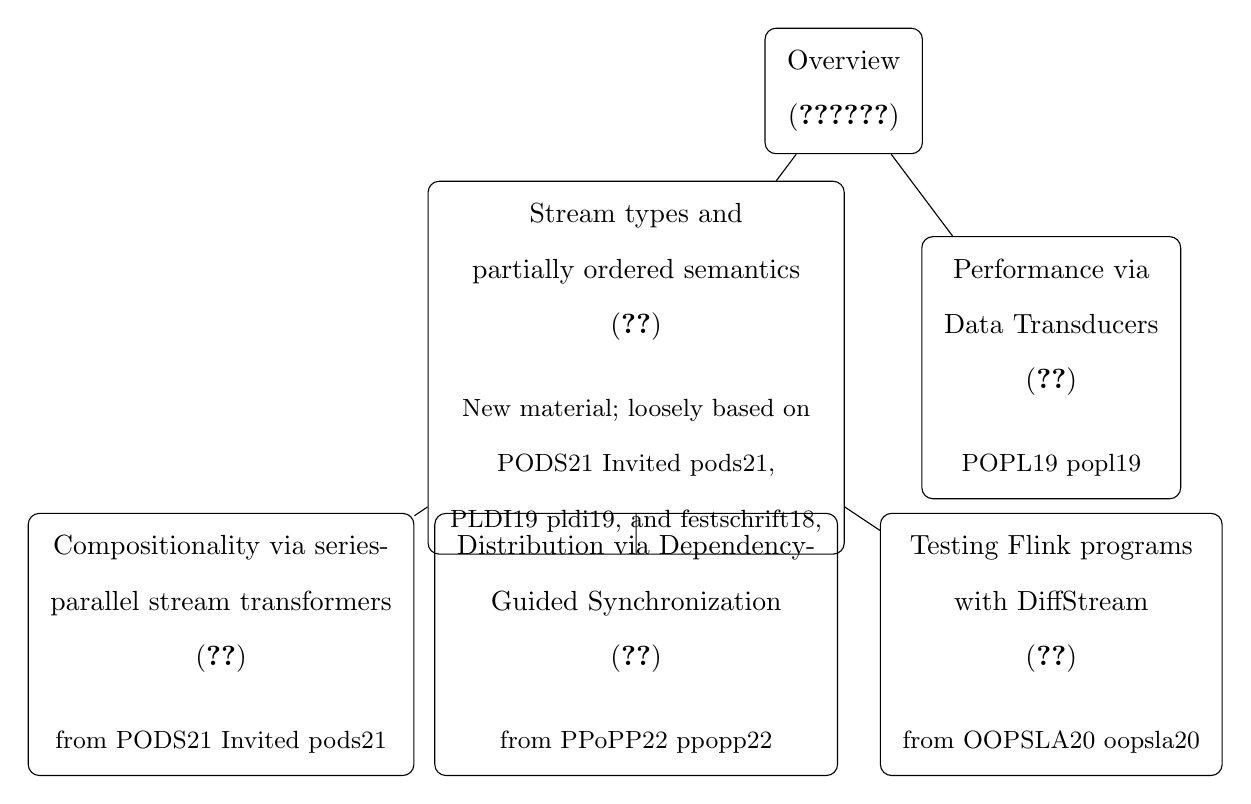
\begin{tikzpicture}[%
    sibling distance=15em,
    level distance=10em,
    every node/.style = {%
      shape=rectangle,
      rounded corners,
      inner sep=0.8em,
      draw,
      align=center
    }
  ]
  \node {
    Overview \\
    (\Cref{cha:intro,cha:background,cha:rw})
  }
    child {
      node {
        Stream types and \\
        partially ordered semantics \\
        (\Cref{cha:foundation}) \\[1em]
        \small New material; loosely based on \\
        \small PODS21 Invited~\citeMain{pods21}, \\
        \small PLDI19~\citeMain{pldi19}, and \citeMain{festschrift18},
      }
      child {
        node {
          Compositionality via series-\\
          parallel stream transformers \\
          (\Cref{cha:composition}) \\[1em]
          \small from PODS21 Invited~\citeMain{pods21}
        }
      }
      child {
        node {
          Distribution via Dependency-\\
          Guided Synchronization \\
          (\Cref{cha:distribution}) \\[1em]
          \small from PPoPP22~\citeMain{ppopp22}
        }
      }
      child {
        node {
          Testing Flink programs \\
          with DiffStream \\
          (\Cref{cha:testing}) \\[1em]
          \small from OOPSLA20~\citeMain{oopsla20}
        }
      }
    }
    child {
      node {
        Performance via \\
        Data Transducers \\
        (\Cref{cha:monitoring}) \\[1em]
        \small POPL19~\citeMain{popl19}
      }
    }
    ;
\end{tikzpicture}

\caption{Overview of the work included in this thesis.}
\label{chapter-overview}
\end{figure}

The structure of the thesis is displayed visually in \Cref{chapter-overview}.
In summary, our contributions are as follows:

\begin{itemize}
\item
We propose a foundational type system for distributed streams based on partially ordered sets.
We show that under our type system, streams can be equivalently viewed as
structured hierarchical data called \emph{batches},
as finite sequences of events called \emph{linearizations},
or as labeled partially ordered sets (traditionally known as pomsets).
In the historical notes, we also discuss how these closely relate to
our earlier synchronization schemas~\citeMain{pods21} and data-trace types~\citeMain{pldi19}.
(\Cref{cha:foundation})

\item
We show how stream operators can be defined compositionally on top of our core type system.~\citeMain{pods21} (\Cref{cha:composition})

\item
We propose \emph{dependency-guided synchronization},
a programming model and system for safe (deterministic and semantics-preserving) distribution~\citeMain{ppopp22}.
(\Cref{cha:distribution})

\item
To detect bugs due to nondeterminism in existing DSPS applications,
we propose \emph{DiffStream}, a differential testing tool~\citeMain{oopsla20}.
In particular, we leverage the partial order viewpoint to specify
ordering requirements, and we test for violations at runtime.
(\Cref{cha:testing})

\item
Towards streaming applications with predictable performance,
we propose \emph{data transducers}, a monitoring formalism and state-machine based intermediate representation~\citeMain{popl19}.
Our formalism is compositional, enabling compilation of high-level
monitoring queries with provable performance bounds.
(\Cref{cha:monitoring})
\end{itemize}

Finally, \Cref{cha:discussion}
contains limitations, unanswered questions, and concluding remarks.

\section{Software}

The work in this thesis is implemented in a number of open-source tools available on GitHub.
\begin{samepage}
\begin{itemize}
\item \githubref{https://github.com/angelhof/flumina}{Flumina} is a parallel programming model for stream processing with safe distribution, written in Erlang with experiments against Flink and Timely Dataflow.
\item \githubref{https://github.com/fniksic/diffstream}{DiffStream} is a differential testing tool for Apache Flink.
\item \githubref{https://github.com/cdstanford/data-transducers}{Data Transducers} is an intermediate representation for streaming with formal performance guarantees, written in Rust.
\end{itemize}
\end{samepage}

\section{Attribution}

Most of the work presented in this thesis was done in close collaboration with my advisor, Rajeev Alur, and other coauthors:
particularly Konstantinos Mamouras (for \Cref{cha:monitoring}) and Konstantinos Kallas and Filip Nikšić (for \Cref{cha:distribution,cha:testing}).
I wrote all the included material in \Cref{cha:intro,cha:background,cha:foundation,cha:composition,cha:discussion}, the material on the programming model in \Cref{cha:distribution}, one of the case studies and other miscellaneous sections in \Cref{cha:testing}, and almost all the material in \Cref{cha:monitoring}.
\Cref{cha:background} incorporates material from my WPE-II written report~\citeMain{wpe2} (of which I am the sole author), and \Cref{cha:rw} integrates some text from all of the papers included in the thesis.

The software repositories Flumina and DiffStream are shared projects with my collaborators, Konstantinos Kallas and Filip Nikšić.
For Flumina, I contributed the experiments and infrastructure with Timely Dataflow in Rust, the Smart Home Power Prediction case study, and documentation.
For DiffStream, I contributed the MapReduce case study and documentation.
The Data Transducers development in Rust is solely my own work.

\chapter{Background}
\label{cha:background}
\headerblock{
  \headerquote{The fourth requirement is that a stream processing engine must guarantee predictable and repeatable outcomes.}{Michael Stonebraker, Uğur Çetintemel, and Stan Zdonik in ``The 8 Requirements of Real-Time Stream Processing,'' 2005~\cite{stonebraker20058}}
}

\begin{figure}[tp]
\def\arraystretch{3.7}
\begin{tabular}{c|cccc}
    System & Year & Stable Release & Active? & \makecell{Questions on \\ StackOverflow \\ (as of 2022-06-07)~\cite{stackoverflow-tags}} \\
    \hline
    Aurora
        & 2003~\cite{Aurora} & 2003~\cite{AuroraWeb} & \No{} & \NA{} \\
    Borealis
        & 2005~\cite{Borealis} & 2008~\cite{BorealisWeb} & \No{} & \NA{} \\
    
\includegraphics[align=c,width=3.5cm]{img/systems/storm.png}
        & 2011~\cite{StormInitRelease} & 2022~\cite{Storm} & \Yes{} & 2564 \\
    \rule{0pt}{11ex} % some extra spacing here
    \makecell{
    
\includegraphics[align=c,width=2.5cm]{img/systems/flink.png} \\ \cite{Flink,Flink2015}}
        & 2011 & 2022~\cite{FlinkRelease} & \Yes{} & 6428 \\
    Google MillWheel
        & 2013~\cite{MillWheel} & \NA{} & \No{} & \NA{} \\
    \makecell{
      
\includegraphics[align=c,width=3.5cm]{img/systems/spark.jpg} \\
      (Apache Spark Streaming)
    }
        & 2013~\cite{Spark2013} & 2022~\cite{SparkStreaming} & \Yes{} & 5408 \\
    \makecell{
\includegraphics[align=c,width=3.5cm]{img/systems/samza.png} \\ \cite{Samza,Samza2017}}
        & 2013 & 2020~\cite{SamzaRelease} & \Yes{} & 81 \\
    Timely Dataflow & 2013~\cite{Naiad2013}
        & 2021~\cite{Timely} & \Yes{} & \NA{} \\
    \makecell{
\includegraphics[align=c,width=3.5cm]{img/systems/heron.png} \\ \cite{Heron,kulkarni2015twitter-heron}}
        & 2015 & 2021~\cite{HeronRelease} & \Yes{} & 43 \\
\end{tabular}

\vspace{0.5cm}

\caption{A selection of major distributed stream processing systems.}
\label{fig:dsps-examples}
\end{figure}

\section{Distributed Stream Processing Systems}

Today's de facto programming solution for programming over
distributed streams
is found in \emph{distributed stream processing systems (DSPS)}.
Popular modern DSPS include
Apache Flink~\cite{Flink,Flink2015},
Timely Dataflow~\cite{Timely,Naiad2013},
and Apache Spark Streaming~\cite{SparkStreaming,Spark2013}.
A selection of these and other systems is included in Table~\ref{fig:dsps-examples}.
There are a vast number of DSPS beyond what can be listed here, including many research prototypes as well as actively developed software products in widespread use.
In this chapter, we review the primary defining properties common to DSPS, with a particular focus on the programming model and semantics. We then discuss the limitations of the existing model and systems.

\subsection{Comparison with Batch Processing}

To understand the emergence of DSPS and why traditional software infrastructure
is not sufficient, note that traditional software
is often based on the assumption that
critical data can be stored and then processed later.
For example,
much of large-scale data analytics relies on processing data in large
\emph{batches} (e.g. training a machine learning model daily),
such as via MapReduce jobs~\cite{dean2008mapreduce}.
While batch processing
does take advantage of distributed computing resources,
it does not take advantage of the transient and temporal structure of data.
Data is not transient because it must be stored first,
which introduces costs due to batch sizes and data movement.
In practice due to these costs, most data traveling over the internet
and processed by cloud services is either not stored or not harvested to its full potential.
Additionally, the temporal structure of data is lost in batches, which divide
data at arbitrary boundaries in time.
For example, a machine learning model that might benefit from continuous updates is instead trained only on the data from yesterday.
DSPS offer a software framework for writing such programs, where data processing logic is defined in a platform-independent manner,
then deployed as a distributed application over many nodes.
DSPS performance is measured in terms of \emph{latency} and \emph{throughput},
while batch processing performance is primarily measured in terms of throughput only.
Concretely, stream processing platforms aim for latency in the milliseconds and throughput in tens of thousands of events per process per node.

\section{Commonalities}

While DSPS differ in many substantial ways, all DSPS in current use share the so-called \emph{dataflow programming model.} This means that the programmer writes, in some form or another, a dataflow graph. In some systems, e.g. Apache Storm, the dataflow graph is written out explicitly, whereas in others, such as Apache Flink, the graph is implicit. Additionally, systems may offer high-level libraries for creating or composing dataflow graphs; in particular, these include libraries for complex windowing operations and for SQL- and CQL-based streaming queries.
The dataflow programming model exposes task and pipeline parallelism; to expose additional data parallelism, DSPS use \emph{operator replication}. Similar to how a MapReduce~\cite{dean2008mapreduce} job is implicitly parallelized, all operators in a dataflow grpah (unless configured otherwise) may be split into several copies; this is part of the programming model as well, and affects the semantics.

\subsection{The Dataflow Programming Model}

We introduce the programming model through a simplified example based on a real-time video analytics use case.
Imagine a large-scale system of video cameras, perhaps located in several cities throughout a country. Each video camera produces a stream of video data, at a certain frame rate and image resolution. Suppose that we want to identify pedestrians and report to a central location the summary of all pedestrian activity in the last 10 minutes, i.e., where pedestrians are most active. To do so, we want to classify each image from each camera using an out-of-the-box classifier; then, to prevent noise and to summarize the total activity, we want to aggregate the data from all classifiers in the last 10 minutes in a particular location (e.g., one intersection or group of intersections). In the end, we report for each location the total amount of pedestrian activity. (One could imagine taking further steps, such as adding a smoothing filter which removes reports of pedestrian activity that last only for a single frame, assuming that these must be erroneous.)

A dataflow pipeline for this is given in Figure~\ref{fig:dataflow-example}. The input data consists of raw video data. Notice that the pipeline contains only one operator at each stage; that is, we treat all input data at \emph{all} cameras as a single input stream; and we write transformations over that stream. The first transformation, \texttt{keyBy(deviceID)}, says to divide the stream into substreams for different keys, where each key is a device ID. (Note that in some frameworks, such as Apache Storm, this would not necessarily be an explicit operator in the dataflow, but rather an annotation on the input data streams.) The second transformation, \texttt{classify}, says to process each input data item, which is a video frame, and return the classification ($1$ for a pedestrian, $0$ for no pedestrian). The third transformation is similar to the first, but this time we group by location, instead of by device ID. The final transformation is the sliding window which adds up all the values over the last 10 minutes. This is then output and could be displayed to the user as a real-time report of activity across all locations.

\begin{figure}[t]
\centering
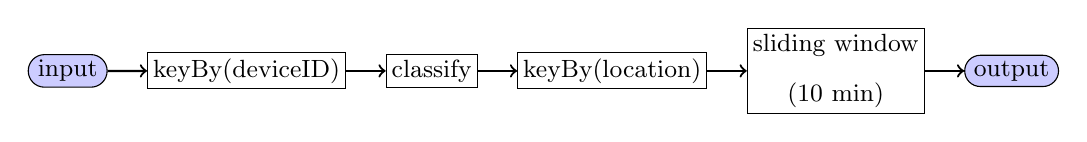
\begin{tikzpicture}[node distance=0.5cm,every node/.style={font=\small}]
\node[source] (in) {input};
\node[operator, right=of in] (op1) {keyBy(deviceID)};
\node[operator, right=of op1] (op2) {classify};
\node[operator, right=of op2] (op3) {keyBy(location)};
\node[operator, right=of op3] (op4) {sliding window \\ (10 min)};
\node[sink, right=of op4] (out) {output};

\draw[dataflowedge] (in) -- (op1);
\draw[dataflowedge] (op1) -- (op2);
\draw[dataflowedge] (op2) -- (op3);
\draw[dataflowedge] (op3) -- (op4);
\draw[dataflowedge] (op4) -- (out);
\end{tikzpicture}

\caption[Example dataflow graph.]{Example DSP dataflow graph for a program to classify video streams and report total pedestrian activity.}
\label{fig:dataflow-example}
\end{figure}

In general, streaming dataflow graphs are acyclic, although some systems support ways to provide feedback and/or support iterative (cyclic) computations.
The input and output nodes in a dataflow are special, because they interact with the external system, and can usually be of several kinds: e.g. taking input from a distributed file system, taking input from a live stream of data, writing output to a file, or in general interacting with some external service which provides input or consumes output.
It is generally preferred that \emph{internal nodes do not consume input or produce output}; however, that does not mean they are pure; they are often stateful, and may also produce logs, interact with a stored database, etc.
Formally, we summarize a definition of a streaming dataflow graph that is (approximately) common to all DSPS programming models.

\begin{definition}[Streaming Dataflow Graph]
\label{def:dataflow-graph}
An \emph{acyclic streaming dataflow graph} (DSP dataflow graph) consists of a set of input nodes called \emph{sources}, a set of intermediate nodes
called \emph{operators}, and a set of output nodes called \emph{sinks}, connected by a set of
directed edges which are \emph{data streams}.
The nodes and edges form a directed acyclic graph (DAG).
Each source node may produce data items continuously, and each sink node consumes data items.

\emph{Operators} are possibly stateful streaming functions that describe how to process an input item and when to produce output. They do not get to choose which of their input streams to read from; rather they have an input even handler which can be called on any event when it arrives.
They may produce any number of outputs on any input item, in any combination of output streams.
\end{definition}

The number of output items produced per input item is often called the operator's \emph{selectivity},
which may be e.g. $1$ (for a map), $0-1$ (for a filter), or more than $1$ (for a copy).
The fact that the selectivity is not constant is a major challenge that makes scheduling DSPS applications more difficult.

\subsection{Auto-Parallelization (Operator Replication)}
\label{bg:autoparallelization}

DSPS rely on three types of parallelization to achieve scalability, especially to achieve high throughput.
The first two are explicitly exposed in any acyclic streaming dataflow graph. \emph{Pipeline parallelism}, which is visible in Figure~\ref{fig:dataflow-example}, means that different operators in a sequential pipeline can be run by different workers, threads, or distributed nodes. \emph{Task parallelism} is not shown in our example, but means that different operators in a parallel set of disjoint tasks (parallel nodes in the dataflow) can be run by different workers, threads, or distributed nodes. However, the arguably most important form of parallelism for huge data sources is \emph{data parallelism}, where different data items in the same input stream are processed by different workers, threads, or distributed nodes.
DSPS use \emph{auto-parallelization} to accomplish data parallelism, and unlike the other two kinds of parallelism, it modifies the dataflow graph and potentially the semantics of the program.

In our example of Figure~\ref{fig:dataflow-example}, we want to exploit data parallelism on video streams from different cameras. In the \texttt{classify} stage of the pipeline, we are classifying images from different cameras separately, so it should be able to be run in parallel.
The problem with data parallelism is that it would be cumbersome for the programmer to expose on their own; they would be forced to explicitly write dozens or hundreds of copies of the \texttt{classify} operator, and manually divide the source into dozens or hundreds of different sources, so that each operator got its own subset of the input data.
To avoid this, DSPS automatically replicate operators in the dataflow graph into several parallel copies. Typically, the number of parallel copies can be configured by the programmer by setting the level of parallelism.

\begin{figure}[t]
\centering
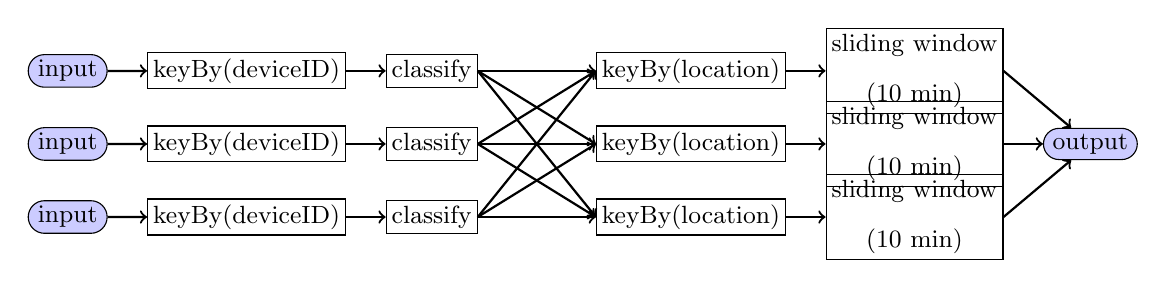
\begin{tikzpicture}[node distance=0.5cm,every node/.style={font=\small}]
\node[source] (in1) {input};
\node[source, below=of in1] (in2) {input};
\node[source, below=of in2] (in3) {input};
\node[operator, right=of in1] (op11) {keyBy(deviceID)};
\node[operator, right=of in2] (op12) {keyBy(deviceID)};
\node[operator, right=of in3] (op13) {keyBy(deviceID)};
\node[operator, right=of op11] (op21) {classify};
\node[operator, right=of op12] (op22) {classify};
\node[operator, right=of op13] (op23) {classify};
\node[operator, right=1.5cm of op21] (op31) {keyBy(location)};
\node[operator, right=1.5cm of op22] (op32) {keyBy(location)};
\node[operator, right=1.5cm of op23] (op33) {keyBy(location)};
\node[operator, right=of op31] (op41) {sliding window \\ (10 min)};
\node[operator, right=of op32] (op42) {sliding window \\ (10 min)};
\node[operator, right=of op33] (op43) {sliding window \\ (10 min)};
\node[sink, right=of op42] (out) {output};

\draw[dataflowedge] (in1) -- (op11);
\draw[dataflowedge] (in2) -- (op12);
\draw[dataflowedge] (in3) -- (op13);
\draw[dataflowedge] (op11) -- (op21);
\draw[dataflowedge] (op12) -- (op22);
\draw[dataflowedge] (op13) -- (op23);
\draw[dataflowedge] (op21.east) -- (op31.west);
\draw[dataflowedge] (op21.east) -- (op32.west);
\draw[dataflowedge] (op21.east) -- (op33.west);
\draw[dataflowedge] (op22.east) -- (op31.west);
\draw[dataflowedge] (op22.east) -- (op32.west);
\draw[dataflowedge] (op22.east) -- (op33.west);
\draw[dataflowedge] (op23.east) -- (op31.west);
\draw[dataflowedge] (op23.east) -- (op32.west);
\draw[dataflowedge] (op23.east) -- (op33.west);
\draw[dataflowedge] (op31) -- (op41);
\draw[dataflowedge] (op32) -- (op42);
\draw[dataflowedge] (op33) -- (op43);
\draw[dataflowedge] (op41.east) -- (out);
\draw[dataflowedge] (op42.east) -- (out);
\draw[dataflowedge] (op43.east) -- (out);
\end{tikzpicture}

\caption{Example dataflow graph after operator replication.}
\label{fig:dataflow-example-parallel}
\end{figure}

On our example, a possible auto-parallelized graph produced by the system is shown in Figure~\ref{fig:dataflow-example-parallel}.
Each operator is replicated, in this case into $3$ copies.
However, this does not fully describe what happens, because we have to understand the connections between operators. If there was an edge before, now there are $9$ possible edges, and the system must decide which of them to use, and how to send data along the edges.

Typically there are several possible strategies, and the system chooses one based on context and/or explicit user configuration. One strategy is \emph{round-robin}, where outputs from one stage of the pipeline are sent to the inputs of the next stage in round-robin order (so for every $3$ outputs from one stage, $1$ gets sent to each of the $3$ operators in the following stage). A second strategy is \emph{key-based partitioning} where the operator copy that an item is sent to depends on (a hash of) a specified key. Finally, in cases where there are the same number of parallel copies from one stage to the next, it is common to \emph{preserve the same partitioning} from one stage to the next.

The partition operator \texttt{keyBy} in our example dataflow graph has no effect except to force a particular strategy for connections between stages: key-based partitioning based on the specified key.
In Figure~\ref{fig:dataflow-example-parallel}, first we assume that the input arrives partitioned by device ID. The \texttt{keyBy} by device ID then preserves such a partitioning. All future operators preserve the same partitioning, except when there is a second \texttt{keyBy} by location -- this operator re-partitions the data based on location instead of device ID.

Formally, we make no assumption about the different DSPS programming models and how they handle connections between stages, except that they should obey any constraints that are explicitly programmed by the user. We capture the allowable parallelization in an annotated DSP graph in the following definition.

\begin{definition}[Annotated Dataflow Graph and Parallelization]
\label{def:dataflow-graph-parallelized}
An \emph{annotated dataflow graph} consists of a dataflow graph annotated with, for each edge, whether the connection between parallel operator replicas should be (1) round-robin, (2) on the basis of a particular key, (3) partition-preserving, or (4) unspecified.
Additionally, each vertex may be labeled with a level of parallelism that is allowed ($1$ for no parallelism).

A \emph{parallelization} of an annotated dataflow graph consists of a larger graph, where:
(i) each vertex is replicated to between $1$ and $i$ copies, where $i$ is allowed level of parallelism; (ii) for each edge between $v$ and $v'$, if $v$ has $i$ copies and $v'$ has $i'$ copies, the connection must be consistent with the annotation. Specifically, (1) for round-robin items should be assigned to each operator in turn; (2) for key-based partitioning there should exist *some* partitioning of the keys such that that partition determines where a data item is sent next; (3) for partition-preserving, we must have $i = i'$ and the connections are one input to one output; (4) for unspecified, each output item from one stage may be sent to any of the operators for the next stage, as the system sees fit.
\end{definition}

\subsection{Streaming Runtime (Fault Tolerance and Scheduling)}

Once given a parallelized dataflow graph, the primary job of a DSPS runtime is to \emph{schedule} workers in a distributed cluster so as to execute all the operators, continuously and in parallel. The goal of the scheduler is to maximally utilize the available distributed resources, and to prevent one task from becoming a performance bottleneck (called a \emph{straggler}).
In the case of stragglers, there are common techniques for the system to respond, e.g. \emph{throttling} and \emph{back-pressure}.

The performance of the system is generally measured in terms of \emph{latency} and \emph{throughput}. Latency is the time it takes for an output item to be produced after the input item which triggered the production arrives in the system. Throughput is total number of input items successfully processed per unit time.
Throughput is often measured as \emph{max throughput}, the maximum input rate the system can handle before it breaks.
Given fixed resources, there is always some limit to how much input the system can handle; so max throughput is always finite. Beyond the max throughput, DSPS offer few guarantees about behavior, and will likely suffer linearly increasing latency, drop data, or crash altogether.

Finally, DSPS runtimes try to provide all of this with a guarantee of \emph{fault-tolerance}. Whenever a worker is assigned to process some set of items from the input stream, the worker may fail. If this occurs, the system must have a way to rewind back to a safe state and re-process those input items, or re-assign them to a new worker. It is challenging to accomplish this in a way that minimizes overhead and also minimizes the time to recovery when experiencing a fault (see~\cite{venkataraman2017drizzle}).

\section{Limitations}
% TODO: this section
% - Rewrite a bit, this is early text
% - Hit on points from the introduction
% - Add bullet point(s) on lack of commonality between different systems (as promised in the introduction)
% - Add a conclusion

\begin{itemize}
\item \emph{Lack of semantics.}
There exists no widely accepted common semantics for distributed stream processing.
DSPS applications are always written as dataflow graphs, and there are other common elements,
but beyond this different APIs make different choices.
For example, Flink's API
assumes that data arrives in-order per-key, whereas Timely's API does not offer this guarantee.
Specific constructs then come with other differences, for example: whether watermarks (indicating stream progress) are explicitly available or implicit;
and
whether side effects are allowed in an operator or whether the system makes no guarantees in the presence of side effects.

% TODO: fix nondeterminism vs. semantics-preserving, should be two different bullets
\item \emph{Nondeterminism.}
Unfortunately, auto-parallelization of stream processing applications
is not semantics-preserving~\cite{xiao2014nondeterminism,schneider2013safe,hirzel2014catalog}~\citeMain{pldi19},
which results in nondeterminism due to ordering of distributed events.
If nondterminism affects the output, it is usually undesirable as it can lead to bugs that are difficult to identify and reproduce.

In practice, many standard operators are not affected by such reordering: e.g.,
commutative, associative reduce operations or stateless maps and filters.
However, most DSPS do not enforce annotations to determine when it is desirable or not~\cite{schneider2013safe}.

\item \emph{Low-level state management.}
DSPS applications are built under the assumption that users should not have to
write state management logic on their own, intsead relying on predefined
dataflow operators (e.g. maps, filters, aggregation, windowing, and SQL query libraries).
In practice, however, some streaming operations require custom logic.
Examples of more complex logic include linear interpolation (fill in missing input data in a temporally dependent manner),
machine learning operators (aggregate and update a statistical model),
and event-dependent windows (form a window with data-dependent start and closing times).
Because of the ubiquity of such manual state management tasks,
popular APIs (including Storm, Flink, and Timely) allow users to program
operators manually, e.g. providing a state type, an initial state, and an
update function for each input tuple.
However, such operators are difficult to program because they must work under
the sharding mentioned above.
Additionally, if the operator requires interaction with an external service or has side effects (e.g. querying a database), state update logic has to be tolerant to unexpected behavior in case of node failures or network communication; yet in practice, users simply ignore these concerns and this results in applications that may crash unexpectedly on a failure.
As a result of these concerns, DSPS developers and researchers generally agree
that better high-level query constructs are needed that alleviate the need for low-level programming.

% TODO: heading where this is a relevant point
% In practice, these challenges are partially addressed by rigorous testing, data validation, and offloading of key functionality such as reliable storage to external services.

\item \emph{Manual parallel programming.}
Related to low-level state management, DSPS also promise a programming framework
where users should not have to parallelize their application themselves.
However, in practice, many applications are highly difficult to parallelize and require low-level constructs: for example, a \emph{broadcast} construct is used to broadcast important shared or global state to other nodes.
Such parallel programming is highly prone to correctness bugs.

\item \emph{Unpredictable performance.}
Because operators and input data are partitioned by the system, users
do not describe explicitly how to partition them.
However, DSPS do not offer any concrete guarantees about the throughput or latency of the runtime.
In particular, unexpected performance bugs arise in the
case that partitioning is not efficient.
For instance, in an example application processing
an input stream of webpage views, if most of the views come from the same website,
partitioning by key fails and results in a performance bottleneck.
To address these bugs requires that we have more reliable performance guarantees.
Ideally, application performance could be estimated statically or in conjunction with runtime profiling.
\end{itemize}

\section{Summary: Our Viewpoint}

Considered as systems, today's stream processing systems are usually quite effective -- thanks to decades of engineering and research advances. They scale automatically across threads and distributed devices, they are high-throughput and meet microsecond-level latency requirements, and they seemlessly execute simple data processing tasks (e.g. windowing, mapping, grouping, and aggregating). Considered as programming languages, however, they fall short of today's standards. If adopted, tools for formal correctness properties (including fine-grained type safety and determinism) could improve the software development process and toolchain in this space.

\chapter{Related Work}
\label{cha:rw}

\headerblock{
  \headerquote{
  The sequence is represented by a function called a \emph{stream}, which is a functional analog of a coroutine\ldots}{William H. Burge, 1975~\cite{burge1975stream}}
  % The conventional while and for loops of structured programming may be composed by a technique of stream processing (analogous to list processing), which results in more structured programs than the originals.
  % This technique makes it possible to structure a program in a natural way into its logically separate parts, which can then be considered independently.

  \headerbreak{}

  \headerquote{Stream processing research, in particular the study of SPSs, can be traced back at least as far as the 1960s, although not always in a form that is immediately recognizable as such today.}{Robert Stephens, 1997~\cite{stephens1997survey}}

  \headerbreak{}

  \headerquote{Of course, the notion of a stream as a programming abstraction has been around for decades...}{Thies, Karczmarek, and Amarasinghe, 2002~\cite{thies2002streamit}}
}

While the previous section discussed the primary programming paradigm in current use for distributed streams and its limitations, this section provides a more general survey of related work. We include dataflow programming paradigms, considered broadly; correctness support for both stream and batch data-processing; and the study of partially ordered traces in concurrency theory. We also survey other paradigms related to streaming (functional reactive programming, concurrent and distributed programming, state machines for streaming, and runtime monitoring). Finally, we include a non-exhaustive list of research on systems problems (distribution, parallelization, optimization, benchmarking, and profiling).

\section{Dataflow Programming}

\subsection{Distributed Stream Processing Systems}

Applications over streaming data can be implemented using
high-performance, fault tolerant distributed stream processing systems (DSPSs), such as
Apache
Flink \cite{Flink2015,Flink2017,Flink},
Storm~\cite{Storm,StormConcepts},
Spark Streaming~\cite{Spark2013,SparkStreaming},
Kafka~\cite{garg2013apache},
Samza~\cite{Samza2017},
Heron~\cite{kulkarni2015twitter-heron,Heron},
and Beam~\cite{Beam};
Timely Dataflow (Naiad)~\cite{Naiad2013,Timely}
and
Differential Dataflow~\cite{mcsherry2013differential};
Microsoft
StreamInsight~\cite{ACGS2011SI}
and Trill~\cite{chandramouli2014trill};
IBM SPL~\cite{HAG2013SPL};
Google MillWheel~\cite{MillWheel} (now replaced by Google Cloud Dataflow);
Amazon Kinesis~\cite{AmazonKinesis};
and early systems such as
Aurora~\cite{Aurora,AuroraWeb},
Borealis~\cite{Borealis,BorealisWeb},
STREAM~\cite{STREAM2004},
and TelegraphCQ~\cite{Telegraph}.\footnote{
  Some relational database systems also support a limited form of streaming;
  for instance, streaming SQL in Apache Calcite~\cite{begoli2018apache,CalciteStreaming} and Streaming Columns in Apache Derby~\cite{DerbyStreaming}.
}
Stream processing is closely related to,
and sometimes synonymous with,
distributed event processing~\cite{DEBS2006}
and complex event processing~\cite{CEP2006}.
See~\cite{babcock2002models} for an early (2002) report on the status of the field.
See also~\cite{stephens1997survey} for an even earlier (1997) report from the perspective of dataflow languages and reactive systems.

The core programming model for DSPSs is typically based on dataflow with auto-parallelization, as discussed in~\Cref{cha:background},
and this is the primary point of comparison for this thesis.
However, there are other programming models used for streaming, including
high-level query languages (often based on SQL),
extensions to the dataflow model,
and extensions to stream parallelism and distribution.

\subsection{High-level Query Languages}

High-level query languages for streaming include
CQL~\cite{arasu2003cql,ABW2006CQL},
CACQ~\cite{CACQ},
CEDR~\cite{BGAH2007CEDR},
Streaming SQL~\cite{jain2008towards,begoli2019one},
SamzaSQL~\cite{pathirage2016samzasql},
Structured Streaming~\cite{armbrust2018structured},
and StreamQRE~\cite{StreamQRE}.
These languages have existed since the early history
of streaming research from the databases community~\cite{stonebraker20058}.
They offer the promise of convenience and clean semantics, but they can be expressively limited for some use cases (e.g., the value-barrier example discussed in the introduction), as we discuss in~\citeMain{ppopp22}.
They typically offer type-safety with respect to the relational schema of each stream and determinism with respect to processing order --
though there are cases where determinism is not guaranteed, including some possible implementations of CQL's tuple-based windows where ties must be broken arbitrarily.\footnote{Thank you to Phillip Hilliard for this observation.}
Traditional query languages view streams in the \emph{sequence-of-relations} model popularized by CQL, which is limited in expressiveness compared to general partial orders.
Inherently sequential operators, such as tuple-based windows and interpolation, are awkward in the sequence-of-relations model.

In modern systems, query operators (typically including maps, windows, filters, joins, and aggregates)
are often implemented not as a separate stream management platform but as
operators on top of the core dataflow programming model, which can also support custom stateful processing and where data need not conform to the relational schema viewpoint.
The upshot of this two-layered design is that the parallelism present at the core dataflow programming model level is relevant even for query languages as: (i) it dictates the extent to which streams can be distributed and optimized, and (ii) it forces semantic requirements on the query in case determinism is required, as otherwise distribution will not be semantics-preserving.

\subsection{Traditional Dataflow Networks and Synchronous Languages}

Dataflow programming predates stream processing.
Dataflow programming as a solution to parallel and distributed computing
originated with Kahn Process Networks~\cite{gilles1974semantics} (KPN), a deterministic dataflow model based on the restriction that channels are FIFO queues with blocking reads and non-blocking writes. Today's systems wish to offer on-demand processing and avoid arbitrary buffering, so they typically do not implement the KPN approach for streams.
In addition to general KPNs, one restriction of KPNs has been particularly influential: synchronous dataflow~\cite{lee1987synchronous}, which further restricts the FIFO queues so that a fixed number of items are read and written on each cycle of an operator. StreamIt~\cite{thies2002streamit} shows that the synchronous dataflow restriction enables aggressive optimization and scheduling; it also somewhat alleviates the problem with blocking reads, because the presence or absence of input and output items is always known statically.
Similar to StreamIt,
the work on synchronous languages from the 90s including LUSTRE~\cite{halbwachs1991synchronous} and ESTEREL~\cite{berry1992esterel} (see~\cite{BCEHlGdS2003SL} for an overview) benefits from the assumption of
synchrony.

The problem with traditional synchronous dataflow languages is that they cannot implement operators which produce a non-static number of output items in response to an input -- including the very most basic such operator, \emph{filter}. (The filter operator applied to an input stream discards items that do not match a given predicate.) As a result, the synchronous model is generally considered too restrictive today for general streaming~\cite{schneider2013safe}.

\subsection{Modern Dataflow Languages}

A more modern take on dataflow programming is MapReduce online~\cite{condie2010mapreduce}; this exemplifies the viewpoint that streaming dataflow graphs are like MapReduce operators chained together.
Other works on streaming specifically focusing on the programming model include SPADE~\cite{gedik2008spade} and Brooklet~\cite{soule2010universal}.
SPADE supports a fixed list of useful operators for streams, like tuple-level transformations (map, flat-map, filter), aggregations, and streaming joins or barriers; it also incorporates some punctuation-related operators.
Brooklet is more like imperative programming,
and is extremely general: it allows translations from CQL, StreamIt, and a (non-streaming) MapReduce like language called SawZall~\cite{pike2005interpreting}.
Another non-streaming, but popular, MapReduce-based dataflow language
is FlumeJava~\cite{chambers2010flumejava}.

\subsection{Extensions to the Dataflow Model}

The dataflow model is limited in its ability to express iterative or recursive queries and other queries with periodic synchronization between nodes, leading to various extensions focused on better expressiveness.
Naiad~\cite{Naiad2013,Timely} proposes \emph{timely dataflow} in order
to support iterative computation.
We compare closely with Timely, the implementation of timely dataflow in Rust, in \Cref{cha:distribution}.
In brief, though Timely is very expressive it is also often quite low-level; as a result, it falls short of automatically scaling without high-level design sacrifices (exposing implementation details to the user).
To avoid semantic issues with out-of-order data,
Timely makes a simplifying assumption that all events are unordered.
However, this also necessitates extraneous buffering, complicating the programming model in cases where order would be known between events.

As data processing applications are becoming more complex, evolving from
data analytics to general event-driven applications, some stream
processing and database systems are moving from dataflow programming to more
general actor models
\cite{CarboneFKK20,Bernstein19,BernsteinDKM17,Das2018,xu2021move}.
For example, Flink has recently released Stateful Functions,
an actor-based programming model running on top of Flink
\cite{AkhterFK19,StatefulFunctions}.
Actor models are very expressive, but computations need to be implemented manually as
message-passing protocols.

Other extensions to the dataflow model focus on enabling forms of synchronization between nodes or other concurrency control, or communication with external state.
Communication between parallel nodes is disallowed in the usual formulation of dataflow auto-parallelization.
For example, S-Store and TSpoon~\cite{meehan2015s,affetti2020tspoon} extend stream processing systems with online transaction processing, which can implement concurrency control,
and Noria~\cite{gjengset2018noria} and Nova~\cite{zhao2021timestamped} extend stream processing systems with abstractions for operators to access shared state.
Another way to deal with the problem of communication between nodes
is to use \emph{broadcast state}, a low-level messaging mechanism present in
Timely~\cite{BroadcastStateTimely} and Flink~\cite{BroadcastStateFlink}
which lets one node broadcast a message to all other parallel nodes.
We discuss our alternative solution to all of these issues related to concurrency and synchronization in \Cref{cha:distribution}.
In brief, our model avoids sacrificing high-level design by making the distribution of a program independent of the programming model; we guarantee that, subject to an assumption that the the program satisfies some consistency conditions, the implementation is deterministic.

\subsection{Summary}

In all of the existing works on dataflow surveyed, streams are typed at a coarse-grained level: typically, only using a construct such as \texttt{Stream<T>} for a stream of events of type \texttt{T}, and not encoding the possible parallelization.
Some languages include a few variants, such as Flink's \texttt{KeyedStream} which is parallelized by key, and CQL's distinction between streams \texttt{Stream<T>} and time-series relations \texttt{Relation<T>} which are created from streams using windowing operators.
Compared to coarse-grained stream types, fine-grained stream types
record additional parallelization information and describe the possible parallelization at the system level, the dataflow model level, or at the query language level.

\section{Correctness Support for Data-Parallel Programs}

\subsection{Testing}

Many previous works focus on batch processing programs written in the MapReduce~\cite{dean2008mapreduce} framework \cite{csallner2011new,xu2013semantic,marynowski2012testing,chen2016commutativity} (see also the recent survey \cite{moran2019testing}).
Some work~\cite{xu2013testing} goes beyond batch processing to study testing semantic properties of operators in general dataflow or stream-processing programs.
One limitation of many of these works \cite{csallner2011new,xu2013semantic,xu2013testing,chen2016commutativity} is that real-world MapReduce programs (and, by extension, aggregators in stream processing programs) can be non-commutative: the empirical study at Microsoft~\cite{xiao2014nondeterminism} reports that about 58\% of 507 user-written reduce jobs are non-commutative, and that most of these are most likely not buggy.
The previous work on testing would erroneously flag these programs as containing bugs due to nondeterminism (a false positive).

Differential testing~\cite{mckeeman1998differential,groce2007randomized} is a well-established, lightweight, black-box method to detect bugs in complex programs by simply comparing two programs that are supposed to be equivalent.
In \Cref{cha:testing} (DiffStream), we adopt differential testing to finding bugs due to parallelism with the goal of avoiding the false-positives mentioned in the previous paragraph; we do succeed in avoiding false positives in most cases, though not in a few others where nondeterminism is truly inherent to the computation.

Besides DiffStream, a few other dedicated testing tools for Flink now exist:
Flinkspector~\cite{flinkspector} provides unit testing;
FlinkCheck~\cite{espinosa2019flinkcheck} uses temporal logic for property-based testing; and SPOT~\cite{ye2021spot} uses symbolic execution to improve path coverage.
See also~\cite{joachim2018methodology} for further reading on this topic.

\subsection{Static Verification}

In addition to testing -- a dynamic method of checking
correctness -- there has also been research on the static verification
of data-parallel programs. Recent work focuses on the verification of
parallel aggregators that are used in MapReduce programs; methods include automated verification and synthesis of \emph{partial
aggregators} given an aggregation function~\cite{liu2014automating},
or parallelizing user defined aggregators using symbolic
execution~\cite{raychev2015parallelizing}.

We would be interested if similar ideas could be generalized to the abstractions in this thesis,
rather than just MapReduce programs;
i.e., we would like to verify and synthesize operators in streaming dataflow graphs.
Note that streaming graphs are not always decomposable into aggregators, and their parallel
and sequential implementations might have significant structural
differences (see the Topic Count case study in
\Cref{cha:testing}), implying that the parallel implementation cannot be simply
derived from the sequential implementation.

For general stream processing, \cite{schneider2013safe} has proposed an approach to ensure correct parallelization (deterministic distribution) based on categorizing operators for properties such as statefulness and selectivity.
This is very closely related to our work on guaranteeing type-safe, deterministic distribution;
while it is practical, it could be considered ad hoc to enumerate operators into finitely many categories.
Another complication is if considering streaming graphs that interact with external service (e.g., querying a Redis database) or complex extensions to the dataflow model including operators like broadcast-state.

Instead of verifying user-written streaming programs, one can instead consider the problem of correctness for systems, compilers, and implementations.
Towards testing functional correctness of a stream processing system implementation, a framework has been proposed for Microsoft StreamInsight~\cite{raizman2010extensible}.

Overall, verifying streaming dataflows statically is an important problem for future work which is not yet easily within our reach, and which we discuss further in \Cref{cha:discussion}.

\subsection{Empirical Studies and Debugging}

Complementary to directly establishing the correctness of user-written programs, one can look at the problem of correctness from an empirical and engineering perspective.
There are a number of empirical studies which aim to classify bugs in real-world stream- and batch-processing programs. Of these, most~\cite{schroeder2009large, kavulya2010analysis, li2013characteristic, zhou2015empirical} have primarily focused on sources of job failures (e.g., system crashes) or performance issues (e.g., memory use patterns and computational bottlenecks), which are orthogonal to semantic bugs which can be found by testing. The Microsoft study~\cite{xiao2014nondeterminism} is the only study we are aware of that classifies semantic bugs in user-written programs.
In addition to these studies of data-processing programs, there have been some empirical studies which interview users about their testing and debugging needs. In~\cite{fisher2012interactions}, users of Spark are interviewed about tools that would be useful to them, but the study focuses on \emph{human-computer interaction} needs such as data visualization and debugging tools. The more recent study~\cite{vianna2019exploratory} aims to determine how current specialists in data stream processing applications currently implement testing. Most specialist employ unit and integration testing, together with some techniques and tools for more sophisticated testing (e.g., inducing node failures). Our work is motivated by the need to go beyond these standard techniques to increase confidence in the \emph{semantic correctness} of user-written programs, especially in the presence of parallelism and out-of-order data.

Empirical studies can motivate work on visualization and debugging.
Visualization includes generating example inputs for dataflow programs showcasing typical semantic behavior~\cite{olston2009generating}. Debugging includes, e.g., setting up breakpoints, stepping through computations, and determining crash culprits~\cite{gulzar2016bigdebug,olston2011inspector}.

\section{Partially Ordered Trace Theory}

\subsection{Mazurkiewicz Traces}

Our type system builds on foundational work in concurrency theory dating back to Mazurkiewicz \cite{mazurkiewicz1986trace}, where partially ordered sets of events are called \emph{Mazurkiewicz traces}. Mazurkiewicz traces have been studied from the viewpoints of algebra, combinatorics, formal languages and automata, and
logic \cite{DiekertR1995}. In practical applications to verification and
testing of concurrent systems, they appear for example in relation to
\emph{partial order reduction}~\cite{God96,Peled94}, a technique for
pruning the search space of possible execution sequences.

Mazurkiewicz traces correspond to the view of streams as linearizations and as labeled partially ordered sets (see \Cref{cha:foundation}),
traditionally called \emph{partially ordered multisets} (pomsets).
Both of these views and the isomorphism between them are standard and well-known in this literature.
Our type system, however, is an abstraction on top of Mazurkiewicz traces; it
gives rise not to all dependence relations, but only to certain ones that have a series-parallel structure
(see \Cref{prop:stream-types-less-general}).
We believe that the series-parallel streams constitute most useful use cases in practice, where there are usually only perhaps one or two levels of nesting in the type. Most streams consist of events of maybe one or two base types, with punctuation and other system events, and our types aim to cater towards these simpler use cases.

An important technical difference is that in the theory of Mazurkiewicz traces, one usually assumes a finite, symmetric, and reflexive dependence relation~\cite{DiekertR1995}. In contrast, in this thesis, we only require it to be symmetric; it is neither finite (due to arbitrary infinite base-types and key-based parallelism) nor reflexive (due to the relational base type). This is in order to support user-provided dependence relations over a possibly infinite data domain, which is necessary to model common patterns in the streaming setting. Patterns such as this one cannot be captured by a finite alphabet, and this limits the direct application of classical work on concurrency theory over a finite dependence relation.

\subsection{Checking Properties of Traces}

Much classical research has focused on deciding properties of traces such as serializability, linearizability, sequential consistency, and data race detection.
Broadly speaking, these properties are search problems: the algorithm monitors an execution of events, and it must decide if there exists some possible equivalent execution that witnesses the desired property. For example, race detection involves deciding, given a sequence of events, if there is a valid reordering of the events, subject to the constraints imposed by synchronization events, in which two specific events (representing a potential race condition) get reordered. If there are an arbitrary number of threads then race detection is NP-hard~\cite{netzer1990complexity,netzer1992race}
(but it is easy to decide for, say, only two traces and can be done in a streaming manner).
Similarly, checking sequential consistency of a given trace is NP-complete~\cite{gibbons1992complexity},
as is checking linearizability in general~\cite{gibbons1997testing}.
Practical tools for testing correctness of traces (e.g., \cite{savage1997eraser,park2011efficient,sen2008race,wing1993testing,burckhardt2010line,lowe2017testing}) are bound by these results and explore the trade-off between soundness, completeness, and tractability.

In our work we don't generally consider algorithmic problems on traces, with the exception of \Cref{cha:testing},
where we consider the algorithmic problem of checking \emph{equivalence} of two Mazurkiewicz traces (equality of streams up to re-ordering).
As with our type system, we consider this problem for general infinite-alphabet traces, rather than just those over a finite alphabet.
The problem we consider is in PTIME (for the offline variant), admits a space-optimal (though not space-bounded) online monitoring algorithm,
and to our knowledge hasn't been explicitly articulated in existing work on Mazurkiewicz traces.

\section{Other Paradigms}

\subsection{Functional Reactive Programming}

In the functional programming community, researchers have long investigated
\emph{functional reactive programming} (FRP)~\cite{wan2000functional,nilsson2002functional}.
See also~\cite{bainomugisha2013survey} for a survey and~\cite{blackheath2016functional} for an introductory textbook.
FRP is closely related to dataflow and is suitable for streaming.
The earliest work on FRP dates back to the late 1990s, targeted for interactive graphics applications~\cite{elliott1997functional,elliott1997modeling},
but FRP has persistently inspired new formalizations and implementations~\cite{courtney2001frappe,cooper2006embedding,foster2011frenetic,perez2016functional}.
In FRP, streams are mostly sequential objects which are processed incrementally; FRP abstracts both discrete-time and continuous-time signals.
Some research has endeavored to make FRP distributed,
for example by adding mechanisms for
fault tolerance~\cite{perez2020fault},
type-safe clocks~\cite{barenz2018rhine}
and distributed actors~\cite{shibanai2018distributed}.

\subsection{Fork-Join Based Concurrency}

Fork-join based
concurrent programming~\cite{frigo1998implementation,lea2000java}
constitutes a classical parallel programming paradigm,
relevant to \Cref{cha:distribution}.
Fork-join parallel programming models are typically expressive but low-level, and do not guarantee determinism or data-race freedom.
Concurrent revisions~\cite{burckhardt2010concurrent}
guarantees determinism in the presence of concurrent updates
by allowing programmers to declare types to describe how parallel updates are merged on joins.
More generally, a great many proposals exist to make concurrent programming safe (typically not fully deterministic, but at least data-race free);
we do not attempt to survey them all here,
but for a recent example and related work, see fearless concurrency~\cite{milano2022flexible}.

\subsection{Distributed Programming Models and Consistency}

Monotonic lattice-based programming models,
including Conflict-Free Replicated Data Types~\cite{shapiro2011conflict},
Bloom$^L$~\cite{conway12},
and LVars~\cite{lvars13,lvars14},
are designed for coordination-free distributed programming.
These models guarantee strong eventual consistency,
i.e., eventually all replicas will have the same state.
Partially ordered sets are an important concept in this space
because consistency for replicated data stores
often relies on determining which events are unordered and can be
safely executed without coordination,
and which events require global synchronization between nodes.
For some examples of this distinction,
see RedBlue consistency~\cite{li2012making},
MixT~\cite{milano2018mixt},
Gallifrey~\cite{milano2019tour},
Quelea~\cite{sivaramakrishnan2015declarative},
CISE~\cite{gotsman16},
Carol~\cite{lewchenko2019sequential},
Hamband~\cite{houshmand2022hamband},
and Quark~\cite{kaki2022runtime},
all of which support a mix of consistency guarantees on different operations,
effectively inducing a partial order of data store operations.

\subsection{State Machines for Data Processing}

Returning from the distributed to the sequential setting,
next we survey state-machine representations for performance-sensitive
data stream processing, relevant to \Cref{cha:monitoring}.

Deterministic and nondeterministic finite-state automata~\cite{rabin1959finite} are foundational in streaming as they correspond precisely to finite-memory, finite-time-per-element computations. However, they lack the ability to perform \emph{quantitative} computations that aren't finite-state, such as e.g., simply counting the total number of input items.
The simplest studied model of quantitative finite-state computation is
\emph{weighted automata}~\cite{ABK2011WA,DKV2009HWA}, originally defined by Schützenberger \cite{S1961WA}.
Weighted automata extend nondeterministic finite-state automata by annotating transitions with \emph{weights} (which are elements of an abstract semiring) and can be used for the computation of simple quantitative properties, such as counting or summing the input items.
Extensions of weighted automata include \emph{nested weighted automata} \cite{CHO2015NWA}, which allows one level of nesting, and our related work~\citeMain{icalp17}, which generalizes this to arbitrary hierarchical nesting, and was a precursor to data transducers (\citeMain{popl19} and \Cref{cha:monitoring}).
See~\cite{CDH2010QL,CHO2016QMA} for further discussion of quantitative models.
Compared to data transducers, weighted automata support a limited set of operations (addition and multiplication in the semiring), rather than an arbitrary family of data types and operations on them.
And while nested models recover some of this expressiveness, they can be cumbersome to work with.

A second approach to augment classical automata with quantitative features has been with the addition of \emph{registers} that can store values from a potentially infinite set. These models are typically varied in two aspects: by the choice of data types and operations that are allowed for register manipulation, and by the ability to perform tests on the registers for control flow.
The literature on data words, data/register automata, and their associated logics \cite{KF1994FMA, NSV2004FSM, DL2009LFQ, BS2010NRDL, BDMSS2011LDW} (and extensions such as register monitors~\cite{FHS2018}) studies words over an infinite alphabet, typically of the form $(\Sigma \times \mathbb{N})^*$,
where $\Sigma$ is a finite set of tags and $\mathbb{N}$ is the set of the natural numbers.
They allow comparing data values for equality, and these equality tests can affect the control flow.
The work on cost-register automata (CRA)~\cite{AdADRY2013CRA} studies what happens when the control and data registers are kept separate by allowing write access to the registers but no testing.
The register model in cost-register automata originated in streaming transducers~\cite{AC2010SST,AC2011STA,AdA2012STT}.
As discussed in \Cref{dt:subsec:dts-and-cras},
data transducers are expressively equivalent to CRAs, but are exponentially more succinct.
Expressively and in logical terms, both CRAs and data transducers recognize the class of \emph{streamable regular transductions}~\citeMain{tcs20}, which can also be defined by monadic second order logic (MSO) or attribute grammars~\cite{EM1999MTT,BE2000}.

A third extension of automata relevant for quantitative computation is symbolic automata~\cite{d2014minimization,veanes2012symbolic-toolkit} and transducers~\cite{veanes2012symbolic,d2013equivalence};
see \cite{d2021automata} for an introduction.
While symbolic automata do not allow all quantitative computations (e.g., adding up a data word of values), because transitions are predicates on input data, they can express some limited examples.
One problem with weighted automata and register automata is that sometimes may lack closure under sequential composition, because sequential composition can be used to express non-regular properties (see~\cite{StreamQRE}, page 699); e.g., we can add up left and right parentheses to accept the Dyck language, or accept sequences of increasing numbers.
Symbolic automata may be helpful to address this limitation.

\subsection{Runtime Verification and Monitoring}

Our work in \Cref{cha:testing,cha:monitoring} contributes to the large body of work on runtime verification~\cite{leucker2009brief,havelund2004efficient} (also known as \emph{runtime monitoring}), a
lightweight verification paradigm which aims to identify bugs in the
output of a program as it is executed, using minimal computational
resources.
(The testing problem we consider is a runtime verification problem, and
the data transducers work is a language that can be used for monitoring applications.)
In typical work on runtime verification, the problem is to detect
violations of a safety property written in a logical specification language.
The specification is translated into a \emph{monitor}, which executes along with the monitored system: it consumes system events in a streaming manner and outputs the satisfaction or falsification of the specification. \emph{Linear Temporal Logic} (LTL) is the most widely used formalism for describing specifications for monitoring.

LTL is rather limited in expressiveness, but has been extended in various ways,
including quantitative extensions.
Metric Temporal Logic (MTL) has been used for monitoring real-time temporal properties \cite{TR2005MTL}. Signal Temporal Logic (STL), which extends MTL with value comparisons, has been used for monitoring real-valued signals \cite{DDGJJS2017}.
Computing statistical aggregates of LTL-defined properties, as in \cite{finkbeiner2002collecting}, is a limited form of quantitative monitoring.
The Eagle specification language \cite{barringer2004rule} can also express some quantitative monitoring properties, since it supports data-bindings.
Quantitative regular expressions are suitable for quantitative and performance-sensitive monitoring~\cite{QRE,StreamQRE,YLMMAL2017NQRE,AAMMR2018}
and can be compiled to CRAs or data transducers.
Finally, the synchronous languages~\cite{BCEHlGdS2003SL} mentioned earlier can also be used for monitoring quantitative data streams.
LOLA \cite{d2005lola,bozzelli2016foundations} is a notable example of a synchronous language designed for runtime monitoring
with close similarity to state-machine based monitors.
RTLola~\cite{faymonville2017real} extends LOLA to the real-time monitoring setting, rather than synchronous monitoring.

In contrast to classical work in runtime verification and monitoring, our core type system in this thesis models program execution traces as partially rather than totally ordered; our ultimate goal is runtime verification abstractions which work on partially ordered streams, for which \Cref{cha:testing} is an initial proposal, handling the simplest case of equality checks between streams.

\section{Selected Systems Challenges}

On the other side of the programming model,
researchers have proposed distribution, parallelization, optimization, benchmarking, and profiling strategies for stream programs.
These can be relevant to the programming model as they affect the sort of semantic guarantees that the system can offer with respect to parallelism;
however, the primary goal of these works is to enable efficient system implementations.

The literature in these areas is vast; we survey only a subset. We especially focus on papers relevant for \emph{geo-distributed} performance optimization~\citeMain{wpe2}: these aim to enable streaming applications over many distributed nodes that don't necessarily all reside in the same central cluster.
This is especially relevant for IoT applications and edge/fog computing~\cite{satyanarayanan2017emergence,dastjerdi2016fog,shi2016edge,villari2016osmotic} (see also programming models such as Mobile Fog~\cite{hong2013mobile-fog})
and for applications where bandwidth is limited~\cite{vulimiri2015global-analytics,chienchun2018videoedge,zhang2018awstream}.

\subsection{Performance Benchmarking and Profiling}

Towards more fine-tuned optimization, researchers have proposed many techniques for analyzing the performance of existing systems.
In particular, streaming benchmarks are invaluable for comparing across systems.
The Yahoo Streaming Benchmark~\cite{yahoostreaming2016} is widely used,
though outdated in some respects, and has motivated more modern benchmark suites~\cite{bordin2020dspbench,lopez2016performance}.
The DEBS Grand Challenge, an annual contest presented by the DEBS conference~\cite{DEBS2006}, is another useful source of more complex tasks and data.
Performance profiling often centers on detecting performance bottlenecks, called stragglers~\cite{liu2020resource,khan2015empirical}.
SnailTrail exemplifies a state-of-the-art system and technique for latency profiling and straggler detection~\cite{hoffmann2018snailtrail}.

\subsection{Operator Placement}

A fundamental problem in distribution of streaming operators, and closely related to the distribution problem considered in \Cref{cha:distribution},
is \emph{operator placement} where the system determines what node to run a stream operator on.
The work~\cite{cardellini2016optimal} uses constraint solving to optimize operator placement relative to network bandwidth and other constraints.
Other than~\cite{cardellini2016optimal}, there are several lines of work in job scheduling, operator placement, and optimization for DSPSs that try to be network-aware in some fashion. Early and influential works include~\cite{ahmad2004network} and~\cite{pietzuch2006network}.
The first~\cite{ahmad2004network} is probably the first to formalize the DSPS operator placement problem, and to explore (1) how network-awareness can lead to more efficient query evaluation, and (2) how there is a trade-off between latency and bandwidth use in this space.
The second~\cite{pietzuch2006network} presents a simple but effective heuristic algorithm which treats the geo-distributed physical nodes as a system of points in a combined latency-bandwidth space, and uses spring relaxation to find a good configuration.
The work~\cite{gu2015general}, similarly to~\cite{cardellini2016optimal}, encodes operator placement as a mixed integer linear program.
There are a number of other related papers on job scheduling~\cite{aniello2013adaptive,xu2014tstorm,eidenbenz2016task,wolf2008soda,fu2019edgewise}, operator placement~\cite{bonfils2004adaptive,tziritas2016improving,rizou2010solving,lakshmanan2008placement},
and resource elasticity~\cite{cardellini2018decentralized,hochreiner2016elastic,cardellini2018optimal,dias2018dsp-survey}.

Researchers have also modified the programming model to allow the programmer to control operator placement.
SpanEdge~\cite{sajjad2016spanedge} is a primitive modification to the dataflow programming model with tasks that should be run globally versus locally.
A system very related to SpanEdge is Geelytics~\cite{cheng2015geelytics}.
It modifies the dataflow programming model with \emph{scoped tasks}, which have a geographic granularity such as by site, by city, by district, or by section, and are similar to SpanEdge's local and global tasks.
Other than these, the paper~\cite{renart2017datadrivenstreamedge} proposes a programming framework for stream processing in a geo-distributed (at the edge) fashion. The programming framework, however, is not based on dataflow, and is more focused on the communication mechanisms between nodes. There is also a large body of work on programming for wireless sensor networks; see the survey~\cite{mottola2011programming-wsn}. In general, the concerns in that domain have been more low-level, related to connections between sensors, mobility of sensors, communication from one sensor to another via short hops, and so on.

\subsection{Stream Degradation}

An even more aggressive technique for optimizing distributed execution is to degrade and approximate streams to reduce what needs to be sent over the network.
The first stream processing system to incorporate general degradation of data streams was JetStream~\cite{rabkin2014jetstream}.
JetStream seeks to limit bandwidth use not just through degradation, but also ``aggregation'', which refers to a data model where data is saved and aggregated by geo-distributed nodes, and only sent when explicitly requested.
AWStream~\cite{zhang2018awstream} uses programming knobs to control the amount of degradation that occurs for video streams (e.g., frame rate reduction, resolution reduction, or some combination) to try to achieve a Pareto-optimal solution between accuracy and bandwidth use. Other systems in this space include WASP~\cite{jonathan2020wasp}.

\emph{Load shedding}~\cite{tatbul2003load,tatbul2007staying} can be seen as a primitive form of stream degradation.
This refers to selectively dropping tuples in response to load that is beyond capacity, in order to maintain availability and good latency while hopefully not losing too much accuracy.
For video data, for instance, load shedding would enable frame rate reduction but would not allow resolution reduction. It is well studied, but less flexible than what is offered by more modern systems like JetStream and AWStream.

\chapter{A Foundation for Streams}
\label{cha:foundation}
\headerblock{
  \headerquote{The purpose of abstracting is not to be vague, but to create a new semantic level in which one can be absolutely precise.}{Edsger W. Dijkstra~\cite{dijkstra1972humble}}

  \headerhide{
    \headerbreak{}

    \headerimage{img/xkcd-standards.png}
  }
}

This section lays the groundwork for the rest of the technical content of this dissertation: we present our core type system for distributed streams.
Our stream types are an abstraction over Mazurkiewicz traces, studied in concurrency theory to model distributed sets of events~\cite{mazurkiewicz1986trace,DiekertR1995}.
They are based on \emph{synchronization schemas}~\citeMain{pods21}, which evolved from earlier work on \emph{data-trace types}~\citeMain{festschrift18,pldi19}.

A stream type $S$ describes the structure of events in the stream;
semantically it will denote a collection of partially ordered traces.
Formally, there are multiple ways to encode and view partially ordered traces.
First, the global view as a strutured batch $\batchtype{b}{S}$.
This is a parsed structure: for example, if $S$ is composed of two stream types in parallel, $S_1$ and $S_2$, then a batch of type $S$ is a pair of a stream of $S_1$ and a stream of $S_2$.
Second, $S$ gives rise to a type for events $\eventtype{e}{S}$,
which are the possible individual elements in the stream.
Third, $S$ gives rise to a type for linearizations of the stream $\lintype{l}{S}$
which are sequences of events.
Finally, $S$ gives rise to a type for partially ordered sets,
$\posettype{p}{S}$, where the partially ordered set is labeled with events in a consistent way.

\section{Stream Types}

\begin{definition}
Let $T$ denote a base type in the following grammar.
A \emph{stream type} is a type defined syntactically by the following grammar:
\[
  S \quad ::= \quad
    \hier{T}{S} \mid
    \parcomp{S}{S} \mid
    \keyby{T}{S} \mid
    \relleaf{T} \mid
    \empstream{}
\]
\end{definition}

We also have the following abbreviation for a sequence of \texttt{T}:
\[
  \seqleaf{T} := \hier{T}{\empstream{}}.
\]

\begin{figure}
  \centering
  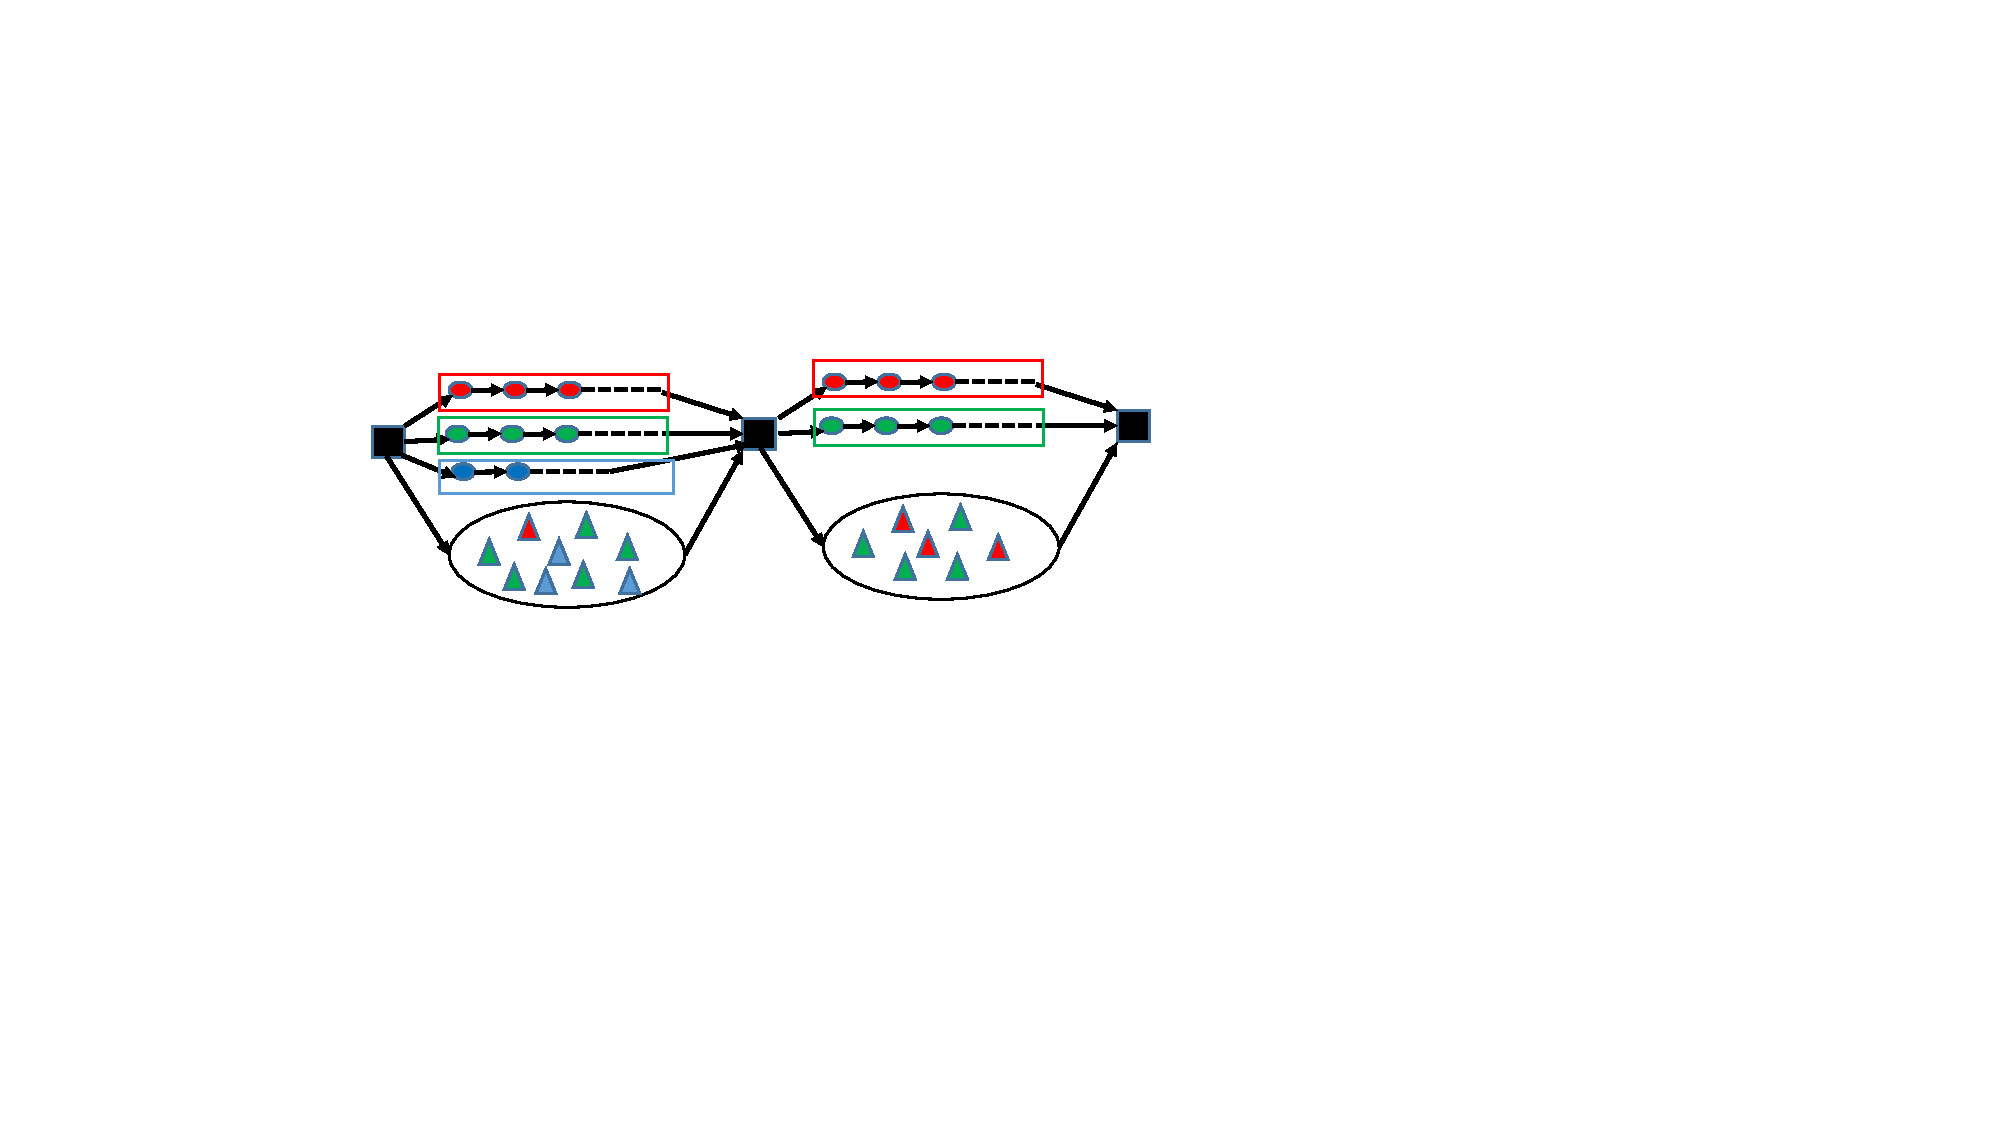
\includegraphics[width=3in]{figures/synchschemas/SPS2.pdf}
  \caption{Illustrative partially ordered stream.}
  \label{fig:ex-postream}
\end{figure}

The idea of this definition is to model partially ordered streams like the one visualized in \Cref{fig:ex-postream}.
This partial order consists of a sequence of black squares $\blacksquare$ with streams in between, which is described by the type $\hier{\blacksquare}{S}$.
The substream type $S$ consists of circles and triangles combined in parallel: $\parcomp{S_1}{S_2}$.
The parallel substream of circles (type $S_1$) consists of a sequences of circles $\bigcirc$, described by $\keyby{K}{\seqleaf{\bigcirc}}$.
The type $K$ in the ParBy construct is a \emph{key} field $K$ that describes the index of the set of substreams (the key on which they are partitioned).
Colors are used to indicate different values of the field $K$
Second, the parallel substream of triangles $\triangle$ is simply a bag, described by $\relleaf{\triangle}$.
Here the colors indicate different values of the base type; note that equal values and unequal values are all parallel in a bag, unlike in ParBy.

Thus, overall, this illustration of a stream is described by the following type:
\[
\hier{\blacksquare}{\parcomp{ \quad \keyby{K}{\seqleaf{\bigcirc}}}{\quad \relleaf{\triangle} \quad}}.
\]

\Cref{45:fig:example-schema} shows this stream type visualized as a tree.
Siblings correspond to the \parcomp{S_1}{S_2} constructor while the rectangular box,
labeled with the key fields, corresponds to the \keyby{K}{S} constructor.
A parent node with several children corresponds to the $\hier{T}{S}$ constructor.

\begin{figure}[t]
  \centering
  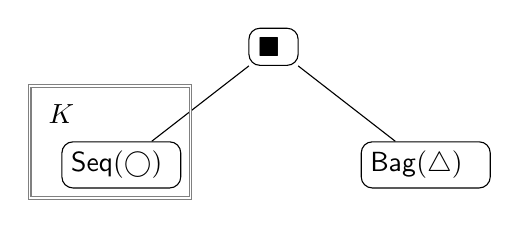
\begin{tikzpicture}[sibling distance=11em,
    every node/.style = {shape=rectangle,
      rounded corners,
      draw, align=center}]
    \node { \TopSchemaNode{ $\blacksquare$ }}
      child {
          \SchemaNode{\seqleaf{ \bigcirc }}{s2}
      }
      child {
          \SchemaNode{\relleaf{ \triangle } }{s3}
      };
    \KeyByNode{$K$}{k1}{s2}{s2};
  \end{tikzpicture}
  \caption{Example stream type for \Cref{fig:ex-postream} drawn as a tree.}
  \label{45:fig:example-schema}
\end{figure}

This example is abstracted, but represents a practical use case such as the following example.

\begin{example}
\label{45:ex:taxi-distance-schema-headers}
\label{45:ex:taxi-distance-schema}
Consider a stream of taxi events, where each is a GPS measurement, an indication of a taxi ride begin or a ride end, or an end-of-hour synchronization marker.
GPS data for each taxi is a tuple type $\bigcirc =$ \texttt{GPS(x: float, y: float, z: float)}, which indicates the type of a GPS measurement using three dimensional coordinates.
Completed ride data is a tuple type $\triangle =$ \texttt{RideCompleted(rideID: int, passengerID: int, cost: int)}.
Finally, end-of-hour events are used to synchronize in time; these are a tuple type $\blacksquare =$ \texttt{EndOfHour(date: date, hour: int)}.

The stream shown in \Cref{fig:ex-postream} applies to this example where squares, circles, and triangles are events of the corresponding tuple types as described above.
The relationship between the different tuple types is described by the stream type shown in \Cref{45:fig:example-schema}.
Described from the bottom up: first, the type $S_1 = \keyby{\texttt{taxiID}}{\seqleaf{\texttt{GPS}}}$ denotes that \texttt{GPS} events are partitioned by the key \texttt{TaxiID} and are totally ordered for each taxi.
Second, $S_2 = \relleaf{\texttt{RideCompleted}}$ denotes that \texttt{RideCompleted} events are unordered, and can be considered to be a bag.
Finally, $S = \hier{\texttt{EndOfHour}}{\parcomp{S_1}{S_2}}$ denotes that \texttt{EndOfHour} events synchronize the events in $S_1$ and $S_2$, each of which can be processed in parallel as they are independent.
\end{example}

The partially ordered structures we have in mind (like the illustration of \Cref{fig:ex-postream}) can be viewed in multiple ways, and we explore this formally in the next subsection.
In particular, we define what it means for a partial order to be a value of type $S$ for a stream $S$ in \Cref{view:labeled-posets}.

\section{Views of Streams}

\subsection{Streams as Structured Batches}
\label{view:batches}

The following syntax defines concrete \emph{structured} stream instances for each of the
stream types, which we call \emph{batches} because they represent data
collected into a static bundle.\footnote{Thanks to Joe Cutler for this suggestion.}
To define a concrete stream instance, one either defines a pair, a sequence, or a bag (unordered multiset).
\[
  B \quad ::= \quad
    (B, B) \mid
    [B, B, \ldots, B] \mid
    \{B, B, \ldots, B\} \mid
    t: T
\]

Batches are typed using the following typing rules:

\begin{mathpar}
    \inference[Synch]
    {
      t_i: T \\
      \batchtype{b_i}{S}
    }
    {
      \batchtype{[b_0, t_1, b_1, t_2, b_2, \ldots, t_m, b_m]}{\hier{T}{S}}
    }
    \\

    \inference[Par]
    {
      \batchtype{b_1}{S_1} \\
      \batchtype{b_2}{S_2} \\
    }
    {
      \batchtype{(b_1, b_2)}{\parcomp{S_1}{S_2}}
    }

    \\

    \inference[ParBy]
    {
      k_i: K \\
      k_i \ne k_j \text{ for } i \ne j \\
      \batchtype{b_i}{S} \emph{ nonempty}
    }
    {
      \batchtype{\{(k_1, b_1), (k_2, b_2), \ldots, (k_n, b_n)\}}{\keyby{K}{S}}
    }

    \\

    \inference[Bag]
    {
      t_i: T
    }
    {
      \batchtype{\{t_1, t_2, \ldots, t_n\}}{\relleaf{T}}
    }

    \inference[Emp]
    {
      \;
    }
    {
      \batchtype{[]}{\empstream{}}
    }
\end{mathpar}

The \emph{nonempty} requirement in the \textsc{ParBy} case is the inductive property that holds exactly when the batch has no occurences of $t: T$ for any base type $T$.
Specifically, $(b_1, b_2)$ is empty if $b_1$ and $b_2$ are empty;
a list is empty if and only if each of its elements is empty;
and a bag is empty if and only if each of its elements is empty.
The batch $t: T$ is never empty.

\subsection{Stream Events and Dependence Relation}
\label{view:events}

A stream can also be thought of as a type for individual events in isolation.
Events can be either base types or tuples.
Tuples are needed because if $K_1, \ldots, K_n$ are types of keys and $T$ is a payload type,
an event is a tuple of an element of each key and an element of the payload.
Here is a grammar for events:
\[
  E \quad ::= \quad (E, E) \mid t: T
\]

We can also talk about events specific to a particular stream type:
$\eventtype{e}{S}$ means that $e$ is a valid event for a stream type $S$.
Notice that there are no rules for $\eventtype{t}{\empstream{}}$ -- there are no events of the empty stream type.

\begin{mathpar}
    \inference[Synch-1]
    {
      e: T
    }
    {
      \eventtype{e}{\hier{T}{S}}
    }

    \inference[Synch-2]
    {
      \eventtype{e}{S}
    }
    {
      \eventtype{e}{\hier{T}{S}}
    }
    \\

    \inference[Par-1]
    {
      \eventtype{e}{S_1}
    }
    {
      \eventtype{e}{\parcomp{S_1}{S_2}}
    }

    \inference[Par-2]
    {
      \eventtype{e}{S_2}
    }
    {
      \eventtype{e}{\parcomp{S_1}{S_2}}
    }

    \\

    \inference[ParBy]
    {
      k: K \\
      \eventtype{e}{S}
    }
    {
      \eventtype{(k, e)}{\keyby{K}{S}}
    }

    \inference[Bag]
    {
      e: T
    }
    {
      \eventtype{e}{\relleaf{T}}
    }
\end{mathpar}

However, a stream type is more than just its type of events.
In addition, a stream defines a \emph{dependence relation}, a symmetric binary relation
on pairs of events.
The relation indicates whether the events should be considered ordered with respect to each other.
For example, in \Cref{fig:ex-postream}, red circles are dependent with each other but independent of green circles;
all circles are dependent with black squares.
One quirk of this model is that because partial orders are transitive,
red circles in on the left are ordered with green circles on the right,
though they are not dependent;
so the dependence relation indicates forced orderings, but additional
orderings may be derived by transitivity.

The dependence relation
$\deptype{e}{e'}{S}$ means that events $e$ and $e'$ are dependent
with respect to the stream tyep $S$ (the events should in particular satisfy $\eventtype{e, e'}{S}$).
This is defined by the following rules.
Notice that there are no rules for
$\empstream{}$ (because it has no events)
nor for $\relleaf{}$ (because all events in a bag are independent).

\begin{mathpar}
    \inference[Synch]
    {
      t: T \\
      \eventtype{e}{\hier{T}{S}}
    }
    {
      \deptype{e}{t}{\hier{T}{S}} \\
      \deptype{t}{e}{\hier{T}{S}}
    }

    \inference[Sub]
    {
      \deptype{e}{e'}{S}
    }
    {
      \deptype{e}{e'}{\hier{T}{S}}
    }
    \\

    \inference[Par-1]
    {
      \deptype{e}{e'}{S_1}
    }
    {
      \deptype{e}{e'}{\parcomp{S_1}{S_2}}
    }

    \inference[Par-2]
    {
      \deptype{e}{e'}{S_2}
    }
    {
      \deptype{e}{e'}{\parcomp{S_1}{S_2}}
    }
    \\

    \inference[ParBy]
    {
      k: K \\
      \deptype{e}{e'}{S}
    }
    {
      \deptype{(k, e)}{(k, e')}{\keyby{K}{S}}
    }
\end{mathpar}

Inductively, $\deptype{e}{e'}{S}$ is the smallest relation defined by the above rules.
It is symmetric, i.e. $\deptype{e}{e'}{S}$ iff $\deptype{e'}{e}{S}$ by an easy induction on the typing judgment.
If two events $\eventtype{e, e'}{S}$ are \emph{not} dependent, we say they are independent and write
$\indeptype{e}{e'}{S}$.
Dependence is constructive and decidable via the above rules, so we could have alternatively given a typing judgment for $\indeptype{e}{e'}{S}$.
For completeness, such a typing judgment is shown in \Cref{app:typing}.

We also could have given both $\deptype{e}{e'}{S}$ and $\indeptype{e}{e'}{S}$ as a single Boolean-valued function on pairs of events,
i.e. $\event{S} \times \event{S} \to \texttt{bool}$.

\subsection{Stream Linearizations and Equivalence Relation}
\label{view:linearizations}

A \emph{linearization} is a sequence of events:
\[
  L \quad ::= \quad [E, E, \ldots, E]
\]
Notice that each event in the sequence may be different (they may even all have different types).
Linearizations support the operations of concatenation ($\cdot$), the interleaving relation
$\lininterleave{l}{l_1, l_2, \ldots, l_k}$,
meaning that $l$ consists of $l_1, l_2, \ldots, l_k$ interleaved in some order.
% and the element-wise product: for $t: E$ and $e_i: E$,
% \[
%   t \times [e_1, e_2, \ldots, e_n] := [(t, e_1), (t, e_2), \ldots, (t, e_n).
% \]

Linearizations are typed using the rule that \emph{a linearization has type $S$ if all its elements are events of $S$}:
\begin{mathpar}
    \inference[Lin]
    {
      l = [e_1, e_2, \ldots, e_n] \\
      \eventtype{e_i}{S} \text{ for all } i
    }
    {
      \lintype{l}{S}
    }

    % \inference[Synch]
    % {
    %   t_i: T \\
    %   \lintype{l_i}{S} \\
    %   l = l_0 \cdot [t_1] \cdot l_1 \cdot [t_2] \cdots [t_m] \cdot l_m
    % }
    % {
    %   \lintype{l}{\hier{T}{S}}
    % }
    %
    % \\
    %
    % \inference[ParBy]
    % {
    %   k_i: T \\
    %   \lintype{l_i}{S} \\
    %   l_i \ne [] \\
    %   \lininterleave{l}{k_1 \times l_1, k_2 \times l_2, \ldots, k_n \times l_n}
    % }
    % {
    %   \lintype{l}{\keyby{T}{S}}
    % }
    %
    % \\
    %
    % \inference[Par]
    % {
    %   \lininterleave{l}{l_1, l_2} \\
    %   \lintype{l_1}{S_1} \\
    %   \lintype{l_2}{S_2} \\
    % }
    % {
    %   \lintype{l}{\parcomp{S_1}{S_2}}
    % }
    %
    % \\
    %
    % \inference[Bag]
    % {
    %   t_i: T
    % }
    % {
    %   \lintype{[t_1, t_2, \ldots, t_n]}{\relleaf{T}}
    % }
    %
    % \inference[Emp]
    % {
    %   \;
    % }
    % {
    %   \lintype{[]}{\empstream{}}
    % }
\end{mathpar}

% No longer needed
% \begin{proposition}
% \label{prop:lin-event-correspondence}
% \begin{enumerate}
% \item Linearizations are the same as sequences of events:
% for any stream type $S$ and sequence $l = [e_1, e_2, \ldots, e_n]$,
% \[
% \lintype{l}{S} \quad \text{iff} \quad \eventtype{e_i}{S} \text{ for all } i.
% \]
% \end{enumerate}
% \end{proposition}
% \begin{proof}
% \end{proof}

The dependence relation also gives rise to an equivalence relation on linearizations.
This equivalence relation is derived as follows:

\begin{mathpar}
    \inference[Indep]
    {
      \indeptype{e}{e'}{S}
    }
    {
      \equivtype{[e, e']}{[e', e]}{S}
    }

    \inference[Concat]
    {
      \equivtype{l_1}{l_1'}{S} \\
      \equivtype{l_2}{l_2'}{S}
    }
    {
      \equivtype{l_1 \cdot l_2}{l_1' \cdot l_2'}{S}
    }

    \\

    \inference[Refl]
    {
      \lintype{l}{S}
    }
    {
      \equivtype{l}{l}{S}
    }

    \inference[Trans]
    {
      \equivtype{l}{l'}{S} \\
      \equivtype{l'}{l''}{S}
    }
    {
      \equivtype{l}{l''}{S}
    }
\end{mathpar}

We should immediately check that equivalence respects our typing judgment (i.e., equivalence is only defined between well-typed linearizations):
\begin{proposition}
\label{prop:equiv-preserves-typing}
If $\equivtype{l}{l'}{S}$ then $\lintype{l}{S}$ and $\lintype{l'}{S}$.
\end{proposition}
\begin{proof}
By induction on the typing judgment for $\equivtype{l}{l'}{S}$.
The base case \textsc{Refl} and inductive case \textsc{Trans} are immediate.
For the base case \textsc{Indep}, the independence precondition is only defined for events $\eventtype{e, e'}{S}$.
Finally for \textsc{Concat}, we observe that linearizations of type $S$ are closed under concatenation by the definition \textsc{Lin} of $\lintype{l}{S}$,
since it states a condition on each element of the sequence individually.
\end{proof}

The other important thing to check immediately is that concatenation respects equivalence, but we don't need to prove this as this is baked into the definition: in particular, the \textsc{Concat} rule forces this. It says that equivalent linearizations concatenate to get equivalent linearizations.

\subsection{Streams as Labeled Posets}
\label{view:labeled-posets}

A \emph{partially ordered set} $(s, \le)$ is a set $s$ together with a binary relation $\le$ on pairs of elements of $s$ that is reflexive, transitive, and antisymmetric.

A \emph{labeled poset} (traditionally called a \emph{pomset}) of type $X$ is a
partially ordered set $(s, \le)$ together with a labeling function $\ell: s \to X$. We denote this $(s, \le, \ell)$. A labeled poset is different than a poset over $X$ because multiple elements may be labeled with the same element of $X$.
Two posets are \emph{equivalent} if the posets are isomorphic and the isomorphism exactly preserves the labeling $\ell$.

Then we can finally define the last view of streams, as partially ordered sets.
We write
\[
\posettype{(s, \le, \ell)}{S}
\]
if $\ell: s \to \event{S}$ such that the order is consistent with the dependence
relation in the following way:
\begin{enumerate}
\item[(i)] If $\deptype{\ell(i)}{\ell(j)}{S}$ then $i \le j$ or $j \le i$; and
\item[(ii)] No relaxation of $\le$ satisfies (i).
\end{enumerate}

\section{Examples}

We illustrate the different views of streams with the simplest example of values and barriers from \Cref{ex:value-barrier}. The stream type corresponding to this example is
\[
S = \hier{\#}{\relleaf{\texttt{int}}}
\]
where $\#$ denotes a barrier and \texttt{int} denotes a value (integer).
Intuitively, this creates a stream of integers in parallel synchronized by $\#$ markers.
The stream views for this example are as follows:
\begin{itemize}
\item A \emph{batch} of type $S$ in this case is an odd-length list, where every other element is a barrier event. For example:
\begin{align*}
  \batchtype{[\{\}]}{S}& \\
  \batchtype{[\{1, 1, 2\}]}{S}& \\
  \batchtype{[\{1\}, \#, \{2\}]}{S}& \\
  \batchtype{[\{1\}, \#, \{1, 1, 2\}, \#, \{\}]}{S}&
\end{align*}
\item An \emph{event} of type $S$ is either a value or a barrier. Anything is dependent with barrier, but values are not dependent with each other. For example:
\begin{align*}
  \eventtype{1}{S}& \\
  \eventtype{2}{S}& \\
  \eventtype{\#}{S}& \\
  \deptype{1}{\#}{S}& \\
  \deptype{\#}{\#}{S}& \\
  \indeptype{1}{2}{S}&
\end{align*}
\item A \emph{linearization} of type $S$ is a sequence of values and barriers. Two linearizations are equivalent ($\equiv$) mod $S$ if they are the same up to reordering values between adjacent barriers. For example:
\begin{align*}
  \lintype{[]}{S}& \\
  \lintype{[1, 3, 2, 1]}{S}& \\
  \lintype{[1, \#, 2, \#, 3]}{S}& \\
  \lintype{[1, \#, \#, \#, 2, 1]}{S}& \\
  \equivtype{[1, 2]}{[2, 1]}{S}& \\
  \equivtype{[\#, 1, 3, 2, 1, \#]}{[\#, 1, 1, 2, 3, \#]}{S}& \\
\end{align*}
We would \emph{not}, however, have equivalence between $[1, \#]$ and $[\#, 1]$, since $1$ and $\#$ are dependent (don't commute).
\item Finally, a \emph{partial order} of type $S$ consists of a partially ordered set labeled with values and barriers in a consistent way:
\[
\begin{tikzpicture}
  \matrix (m) [matrix of math nodes, column sep=3em, row sep=0.5em]
  {
            &          & |(a3)|1 &          \\
    |(a1)|1 &          &         &          \\
            & |(b1)|\# & |(a4)|2 & |(b2)|\# \\
    |(a2)|3 &          &         &          \\
            &          & |(a5)|1 &          \\
  };
  \path[->]
    (a1) edge (b1)
    (a2) edge (b1)
    (b1) edge (a3) edge (a4) edge (a5)
    (a3) edge (b2)
    (a4) edge (b2)
    (a5) edge (b2);
\end{tikzpicture}
\]
Notice that the barrier $\#$ events are ordered with everything, and the value events are unordered as much as possible (except for their order with $\#$).
Since partial orders are transitive, this also implies some orderings on values; for example, the $1$ and $3$ in the first column are ordered less than the $1, 2, 1$ in the third column.

\end{itemize}

\section{Isomorphism between Views}
\label{sec:isomorphism-between-views}

\subsection{Isomorphism between Batches and Linearizations}

\begin{definition}[Flattening]
    \label{def:batch-flattening}
    Let $S$ be a stream type,
    and let $\batchtype{b}{S}$.
    A \emph{flattening} $l$ of $b$ is any linearization
    defined inductively on $S$ as follows:
\begin{itemize}
\item If $S = \empstream{}$, then $b = []$ and $l$ is a flattening of $b$ if and only if $l = []$.
\item If $S = \relleaf{\mathcal{H}}$, then $b$ is a multiset, and $l$ is a flattening of $b$ if and only if the multiset of events in $l$ equals $b$.
(That is, $l$ contains exactly the same events as $b$ in some order. Assuming $b$ has at least two distinct elements, there will be multiple such flattenings.)
\item In case $S = \hier{T}{S'}$, we have $b = [b_0, t_1, b_1, t_2, b_2, \cdots, t_m, b_m]$ for some batches $\batchtype{b_i}{S'}$.
Then $l$ is a flattening of $b$ if and only if $l = l_0 \cdot [t_1] \cdot l_1 \cdot [t_2] \cdot l_2 \cdot \ldots \cdot [t_m] \cdot l_m$,
where $l_i$ is a flattening of $b_i$ for all $i$.
\item In case $S = \parcomp{S_1}{S_2}$, we have $b = (b_1, b_2)$.
Then $l$ is a flattening of $b$ if and only if $l$ is an interleaving of some $l_1, l_2$ where $l_1$ is a flattening of $b_1$ and $l_2$ is a flattenign of $b_2$.
That is, $\lininterleave{l}{l_1, l_2}$.
\item Finally, in case $S = \keyby{K}{S'}$, we have $b$ is a set with finitely many entries $(v_i, b_i)$ for $i = 1, \ldots, m$.
Then $l$ is a flattening of $b$ if and only if $l$ is an interleaving of the sequences $l_1, l_2, \ldots, l_m$
where $l_i$ is a flattening of $t_i$ for each $i$.
That is, $\lininterleave{l}{l_1, l_2, \ldots, l_m}$.
\end{itemize}
\end{definition}

\begin{proposition}
\label{prop:batch-lin-correspondence}
Let $S$ be a stream type such that all base types in $S$ are unique.
\begin{enumerate}
\item[(1)] For every linearization $\lintype{l}{S}$, there exists a \emph{unique} batch $b$ such that $\batchtype{b}{S}$ and $l$ is a flattening of $b$. Call this batch $b = \parselin{l}{S}$.
\item[(2)] For every batch $\batchtype{b}{S}$, every flattening $l$ of $b$ satisfies $\lintype{l}{S}$.
\item[(3)] For every batch $\batchtype{b}{S}$, there exists at least one flattening $l$ of $b$.
\item[(4)] For two linearizations $\lintype{l_1, l_2}{S}$ we have $\equivtype{l_1}{l_2}{S}$ if and only if $\parselin{l_1}{S} = \parselin{l_2}{S}$
\item[(5)] Finally, if $\batchtype{b}{S}$, then for any two flattenings $l_1, l_2$ of $b$, $\equivtype{l_1}{l_2}{S}$.
\end{enumerate}
\end{proposition}
\begin{proof}
Adapted from Appendix B of~\citeMain{pods21} (Proof of Proposition 14).
By induction on $S$.
For $\relleaf{T}$,
all five conditions state a standard correspondence between a multiset of items and its linearizations.
For $\parcomp{S_1}{S_2}$
and for $\keyby{K}{S_1}$,
we observe that sequences over events $\eventtype{e}{S}$ are interleavings of events each from a subtype,
and all such interleavings are equivalent with respect to $\equiv$, by the rule \textsc{Indep}.
Conversely $\equiv$ only holds between different interleavings of the same two or more sequences up to equivalence, i.e. for parallel composition, if $l \equiv l'$ and $l$ is an interleaving of $l_1$ and $l_2$ and $l_1'$ is an interleaving of $l_2'$, then $l_1 \equiv l_1'$ and $l_2 \equiv l_2'$.
This uses the fact that all base types are unique and can be proven inductively on $\equivtype{l}{l'}{S}$.

The most interesting case is $S = \hier{T}{S'}$.
Here, we essentially apply the idea that $(a \cup b)^{*} = (a^{*} b)^{*} a^{*}$ for languages: in this context $a$ is the type $\event{S'}$ and $b$ is the type $T$.
So a sequence of $\event{S}$ decomposes into a sequence of subsequences over $S'$ delineated by $T$ events, where there is one more subsequence than the number of $T$ events.
Since $T$ events are fully dependent on everything else (rule \textsc{Synch}), this decomposition is not changed by $\equiv$, which can thus be identified with equality on the sequence of $T$ events together with equivalence on each $\event{S'}$ substream.
The definition of flattening reflects this decomposition exactly.
\end{proof}

It is worth noting that \emph{not all} binary relations on pairs of $\event{S}$ arise as a dependence relation $\deptype{e}{e'}{S}$.
In particular, the (symmetric reflexive closure of)
the relations $\{(A, B), (B, C), (C, D)\}$
and $\{(A, B), (B, C), (C, D), (D, A)\}$
do not have a hierarchical structure:
here there is no way to choose a header out of $A, B, C, D$
to be a root node in the stream type.

The following proposition
characterizes exactly the dependence relations arising from stream types, based on these two examples.
\begin{proposition}
\label{prop:stream-types-less-general}
For any stream type $S$, the relation $\mathcal{D}$ ($\deptype{e}{e'}{S}$) is symmetric and reflexive.
It additionally satisfies the following restriction:
$\mathcal{D}$ does not contain the cycle graph $C_4 = \{(A, B), (B, C), (C, D)\}$
or the path graph $P_4 = \{(A, B), (B, C), (C, D), (D, A)\}$ when restricted
to any set of four base types $a, b, c, d$.
\end{proposition}
\begin{proof}
Symmetry and reflexivity are by construction in each type constructor for
$\mathcal{D}$.

Now suppose that we introduce a cycle $C_4$ or path $P_4$.
It cannot have been introduced in the base case $\relleaf{T}$,
% or $\seqleaf{T}$,
nor in parallel composition since $C_4$ and $P_4$ are connected;
nor in $\keyby{K}{S}$ since there are no dependencies across keys.
So it must have been introduced by the $\hier{T}{S}$ construct.
But for either $C_4$ or $P_4$, there is no way to partition (cut) the vertices into those in
$T$ and those in $S$ (with at least one vertex in each partition) such that every event in the first is
dependent on every event in the second.
\end{proof}

\subsection{Concatenation on Batches}

Because batches are isomorphic to linearizations up to equivalence (as just shown in \Cref{prop:batch-lin-correspondence}), we can define concatenation on batches. In particular, if $l_1$ and $l_2$ are linearizations of type $S$,
their concatenation $l = l_1 \cdot l_2$ is a linearization of type $S$,
so it has a unique parsing $\batchtype{\parselin{l}{S}}{S}$.
To show that this lifts to an operation on batches $b_1 \circ b_2$, it remains to show that this is well-defined up to equivalence on linearizations:
\begin{proposition}
\label{batch-concatenation-well-defined}
Batch concatenation $b_1 \circ b_2$ is well-defined and associative: $(b_1 \circ b_2) \circ b_3 = b_1 \circ (b_2 \circ b_3)$.
\end{proposition}
\begin{proof}
By the \textsc{Concat} rule as remarked earlier, $\equivtype{l_1}{l_1'}{S}$ and $\equivtype{l_2}{l_2'}{S}$
then $\equivtype{l_1 \cdot l_2}{l_1' \cdot l_2'}{S}$.
Then consider flattenings $l_1$ and $l_2$ of $b_1$ and $b_2$ respectively;
by \Cref{prop:batch-lin-correspondence} (3), (5),
$l_1$ and $l_2$ are unique up to equivalence;
by the \textsc{Concat} rule the concatenation $l_1 \cdot l_2$ is unique up to equivalence;
and by \Cref{prop:batch-lin-correspondence} (4)
this means $\parselin{l_1 \cdot l_2}{S}$ is the same regardless of the choice of $l_1$ and $l_2$.

Associativity follows by associativity of concatenation on sequences since concatenation respects equivalence.
\end{proof}

\subsection{Isomorphism between Linearizations and Labeled Posets}

Given any stream type $S$, any linearization $\lintype{l}{S}$ gives rise to a labeled poset, which we call $\posetlin{l}{S}$ as follows:
if $l$ has length $n$, then we let $s = \{1, 2, \ldots, n\}$, and we define the labeling function $\ell(i) = l[i]$.
Then we define the ordering as follows:
$i <_{l, S} j$ iff there is some sequence of indices
\[
i = i_0 < i_1 < \ldots < i_m = j
\]
such that each pair adjacent in the sequence is dependent:
\[
\deptype{l[i_0]}{l[i_1]}{S}, \deptype{l[i_1]}{l[i_2]}{S}, \ldots, \deptype{l[i_{m-1}]}{l[i_m]}{S}.
\]

This definition may look opaque, but captures the property that $l[i]$ and $l[j]$ are ordered: it is impossible to reorder them to get $l[j]$ before $l[i]$.
The following proposition justifies this formally:
\begin{proposition}
\label{prop:lin-poset-correspondence}
Let $S$ be a stream type such that all base types in $S$ are unique.
\begin{enumerate}
\item[(1)] Let $\lintype{l_1}{S}$ and $\lintype{l_2}{S}$ be two linearizations.
Then $\equivtype{l_1}{l_2}{S}$ if and only if $\posetlin{l_1}{S_1}$ and $\posetlin{l_2}{S_2}$ are isomorphic.
\item[(2)] Let $\lintype{l}{S}$ be a linearization; then $\posettype{\posetlin{l}{S}}{S}$.
\item[(3)] Let $\posettype{p}{S}$; then there exists a linearization $l$ such that $p$ is isomorphic to $\posetlin{l}{S}$.
\end{enumerate}
\end{proposition}
\begin{proof}
For (1) in the forward direction, what we need to show is that the rules for $\equiv$ preserve poset isomorphism. For the rule \textsc{Indep} the isomorphism switches $e$ and $e'$ in the linearization; this preserves the order because $e$ and $e'$ are not ordered under $<_{l, S}$. \textsc{Refl} and \textsc{Trans} hold because poset isomorphism is transitive. Finally for \textsc{Concat}, we construct an isomorphism between the posets on $l_1 \cdot l_2$ and $l_1' \cdot l_2'$ by combining the isomorphisms on the first half and second half. The idea is then that any ordering in $<_{l_1 \cdot l_2, S}$ defined by $i = i_0 < i_1 < \ldots < i_m = j$ is derived from a first half of orderings in $l_1$, followed by a second half of orderings in $l_2$,
which is isomorphic to a segment of orderings in $l_1'$ followed by a segment of orderings in $l_2'$, which implies ordering in $<_{l_1' \cdot l_2', S}$.
The reverse direction requires decomposing any isomorphism by induction into a matching between the elements of the individual linearizations such that the matchign can be formed by repeated consecutive swaps, implying equivalence via \textsc{Indep}, \textsc{Concat}, and \textsc{Trans}; this is the same as for data-trace types and a full proof can be found in~\citeMain{pldi19} and~\citeMain{festschrift18}.

For (2), the crux of the statement is that our definition of $<_{l, S}$ precisely captures the smallest ordering consistent with dependence $\mathcal{D}$ as described in the definition of a poset. Since $\deptype{l[i]}{l[j]}{S}$ implies that $i <_{l, S} j$ or vice versa, $<_{l, S}$ is an ordering consistent with $\mathcal{D}$, so it remains to see why there is no weaker ordering. But note that any weaker ordering would have to remove $i <_{l, S} j$ for some $i < j$ as these are the atomic constraints generating the ordering, and then it would not be consistent with $\mathcal{D}$.

Finally, for (3), for an arbitrary finite labeled poset $p$ of size $n$ pick any topological ordering of its elements $1, 2, 3, \ldots, n$, and consider the linerization $\lintype{l}{S}$ defined by elements $1, 2, 3, \ldots, n$ in that order. The ordering arising from $p$ must contain all pairs $i <_{l, S} j$ where $\deptype{l[i]}{l[j]}$ because otherwise $i$ and $j$ would be indepdent, violating consistency with $\mathcal{D}$; and it must be the smallest ordering containing these pairs by minimality of $p$.
\end{proof}

\section{Stream Type Relaxation}

We define relaxation, a form of semantic subtyping: $S_1$ is a relaxation of $S_2$ means that a stream of type $S_2$ can be interpreted as a stream of type $S_1$ if the partial order is relaxed.
The following are adapted from Section 2.5 and Appendix B of~\citeMain{pods21}.
We assume some subtyping relation on base types, which can be trivial if unwanted;
in that case the relaxation requires type equality $\event{S_1} = \event{S_2}$.

\begin{definition}[Stream relaxation]
\label{def:stream-relaxation}
For stream types $S_1$ and $S_2$,
$S_1$ is a \emph{relaxation} of $S_2$, written $S_1 \lesssim S_2$, if
(i) $\event{S_1}$ is a supertype of $\event{S_2}$
and (ii) for all tuples $\eventtype{x, y}{S_2}$,
if $\deptype{x}{y}{S_1}$ then $\deptype{x}{y}{S_2}$.

Two stream types $S_1$ and $S_2$ are \emph{order-equivalent}, denoted $S_1 \sim S_2$, if both $S_1 \lesssim S_2$ and $S_2 \lesssim S_1$.
\end{definition}

\begin{proposition}
\label{prop:stream-relaxation-lin}
\label{45:prop:schema-relaxation-flattening}
Suppose that $S' \lesssim S$. Then:
(1) If $\lintype{l}{S}$ then $\lintype{l}{S'}$.
(2) If $\equivtype{l_1}{l_2}{S}$ then $\equivtype{l_1}{l_2}{S'}$.
\end{proposition}
\begin{proof}
Statement (1) is direct from the fact that $\event{S'}$ is a supertype of $\event{S}$
and linearizations are sequences of events.
For (2) all typing rules for $\equivtype{l_1}{l_2}{S'}$ are the same as for $\equivtype{l_1}{l_2}{S}$ except \textsc{Indep}, which introduces strictly more equivalences by condition (ii) of the relaxation.
\end{proof}
% Proof of similar fact for synch schemas but stated in terms of flattenings:
%
% We first show uniqueness. Let $t_1', t_2': S'$
% such that every flattening of $t$ is a flattening of $t_1'$ and of $t_2'$.
% Since every SPS has at least one flattening,
% we can choose some particular flattening $s$ of $t$
% (a sequence over $\headers(S)$).
% By uniqueness in Proposition~\ref{45:prop:sps-sequence-correspondence}-(1),
% since $s$ is a flattening of both $t_1'$ and $t_2'$, $t_1' = t_2'$.
%
% Now we show existence.
% As before, choose a particular flattening $s$ of $t$.
% Since $\headers(S') \supseteq \headers(S)$,
% $s$ is also a sequence over $\headers(S')$.
% Thus by Proposition~\ref{45:prop:sps-sequence-correspondence}-(1),
% there exists a $t': S'$ such that $s$ is a flattening
% of $s$.
% It remains to show that all flattenings of $t$ are flattenings of $t'$.
% Given any flattening $\hat{s}$ of $t$,
% by Proposition~\ref{45:prop:sps-sequence-correspondence}-(2b),
% $s \equiv_{D_{S}} \hat{s}$.
% By the definition of relaxation,
% $s \equiv_{D_{S'}} \hat{s}$.
% Then by Proposition~\ref{45:prop:sps-sequence-correspondence}-(2a),
% $\hat{s}$ is a flattening of $t'$.

\begin{theorem}
\label{thm:stream-relaxation-decidable}
Stream relaxation, that is on input two stream types $S_1$ and $S_2$, checking if $S_1 \lesssim S_2$ (and consequently checking stream type equivalence), is decidable in quadratic time.
\end{theorem}
\begin{proof}
We may ignore the base types in $S_1$ and not in $S_2$.
Then for each pair of base types $T, T'$ in $\event{S_2}$,
we build a formula $\phi^1_{T, T'}$ whose free variables are elements of $T$ and elements of $T'$ or fields of $T$ and fields of $T'$ in case they are tuple types,
which is true exactly when
$\deptype{x}{x'}{S_1}$ for $x : T$ and $x' : T'$.
This is done by expanding out the cases for the dependence relation $D$.
In all case the formula built is either true or false, or a derived from a subcase,
except in the $\keyby{K}{S}$ case where
we get an equality constraint as an atomic formula:
specifically, for $\deptype{(k, e)}{(k', e')}{\keyby{K}{S}}$
we get the constraint $k = k'$ (in conjunction with the recursive formula for $\deptype{e}{S}{S'}$).
Altogether, each $\phi^1_{T, T'}$ is just an atomic formula over the
language of equality.
We do the same for $S_2$ to get formulas $\phi^2_{T, T'}$.

The problem now becomes checking a set of implications
of atomic formulas over the language of equality, which is
decidable by checking each implication
$\phi^1_{T, T'} \to \phi^2_{T, T'}$
in turn.
The complexity is quadratic because there are quadratically many pairs $T, T'$.
\end{proof}

\section{Monotonicity, Type Safety, and Determinism}
\label{sec:operator-properties}

Finally, we define three key properties that are relevant to the rest of the thesis: monotonicity, type safety, and determinism for operators over streams.
First, we need an abstract model of an operator in a stream processing system.
\begin{definition}
An \emph{operator} from type $X$ to type $Y$ is a relation
$F \subseteq \listtype{X} \times \listtype{Y}$ such that each input is associated with at least one output:
for every $l: \listtype{X}$, there exists $l': \listtype{Y}$
such that $(l, l') \in F$.
\end{definition}

Modeling the operator as a relation is necessary because it allows for nondeterministic behavior; that is, this is a model of a concurrent system with multiple possible execution traces. The definition only requires that there is at least one possible behavior on any given input stream.

A bit of foreshadowing: operators are key objects studied in \Cref{cha:distribution,cha:testing,cha:monitoring}.
The functions over batches considered in \Cref{cha:composition} can also be seen as operators (though they aren't directly expressed as such) by applying the isomorphism in \Cref{sec:isomorphism-between-views}.

For the following properties, let $S$ be an input stream type, $S'$ an output stream type, and $F$ an operator from $\event{S}$ to $\event{S'}$.
\begin{itemize}
  \item \textbf{Monotonicity:} $F$ is \emph{monotone}
  if for all $(l, m) \in F$, if $l$ is a prefix of $l'$, then there
  exists $m'$ such that $m$ is a prefix of $m'$ and $(l', m') \in F$.

  \item \textbf{Type safety:} $F$ is \emph{type safe} if, for all $(l, m) \in F$, if $\equivtype{l}{l'}{S}$ then there exists $m'$ such that $\equivtype{m}{m'}{S}$ and $(l', m') \in F$.

  \item \textbf{Determinism:} $F$ is \emph{deterministic up to output equivalence} if, whenever $(l, m) \in F$ and $(l, m') \in F$, $\equivtype{m}{m'}{S}$.
\end{itemize}

\subsection{Examples and notes}

To illustrate monotonicity, the function that takes in a sequence of integers and outputs their sum is not monotonic because on input $[1, 2, 3]$ it produces $[6]$ and on input $[1, 2, 3, 1]$ it produces $[7]$, but $[6]$ is not a prefix of $[7]$. To make it monotonic, we have to add an end-of-stream symbol at the end: the correct function to consider is the one which maps $[1, 2, 3]$ to $[]$, but maps $[1, 2, 3, \#]$ to $6$.
Specifically, we define the function which maps $[a_1, a_2, a_3, \ldots, a_k, \#] + t$ to $[a_1 + a_2 + \cdots + a_k]$ for any integers $a_1, \ldots, a_k$ and any tail list $t$, but maps input lists with no instance of $\#$ to $[]$. This function is monotonic.

To illustrate type safety, consider the identify function: $F$ consists of all pairs $(l, l)$, e.g. it maps $[1, 2, 3]$ to $[1, 2, 3]$.
Suppose $S$ also allows input reorderings, so that $\equivtype{[1, 2, 3]}{[1, 3, 2]}{S}$.
Then type safety says that there should be an output on $[1, 3, 2]$ that is equivalent to $[1, 2, 3]$ under $S'$.
This holds if, and only if, $\equivtype{[1, 2, 3]}{[1, 3, 2]}{S'}$.
So this identity operator is type safe if and only if $S'$ allows output reorderings.

It is possible for a operator to be type safe, but not deterministic. Consider $F$ which maps the list $l = [1, 2, 3]$ to all its possible reorderings: $F$ contains all six pairs
\[
(l, l), (l, [1, 3, 2]), (l, [2, 1, 3]), (l, [2, 3, 1]), (l, [3, 1, 2]), (l, [3, 2, 1]).
\]
Then even if $\equivtype{[1, 2, 3]}{[1, 3, 2]}{S}$ but NOT $\equivtype{[1, 2, 3]}{[1, 3, 2]}{S'}$, this relation is still type safe because the output, while a set of inequivalent possibilities and not just one, doesn't depend on the input.

Why do we call this property ``type safety''? It is analagous to if one defines a function on an input type of integers modulo $5$, the output should not depend on the exact choice of residue class; $f(4)$ and $f(9)$ should be the same (up to output equivalence). Or to take another example, if Booleans are represented as integers where False is $0$ and True is any nonzero integer, Boolean operations are only type safe if they are not defined with respect to the particular choice of representation of True. In our case, $S$ and $S'$ define types with a custom equality relation $\equiv$ on linearizations, and the property encodes the fact that the equalities in the input transfer over to the output. This captures exactly the property necessary for $F$ to be interprable as a relation between input batches and output batches, or between input labeled posets and output labeled posets (see the next subsection).

Finally, determinism.
Note that the property is strictly weaker than saying the relational is functional: we do not require that for any $l$ there is exactly one $m$ such that $(l, m) \in F$, because that would disallow implementations which benefit from parallelism. Instead, the output $m$ only must be unique up to output equivalence: there can be multiple $(l, m)$ and $(l, m')$, but only if $m$ and $m'$ are equivalent. This says nothing about the input equivalence; it is possible for an operator to be deterministic, but not type safe, if it uses the particular choice of input $l$.
For example, consider the last-element function that on $[1, 2, 3]$ returns $[3]$ and on $[1, 3, 2]$ returns $[2]$. This is deterministic because it is a function. But if we have $\equivtype{[1, 2, 3]}{[1, 3, 2]}{S}$, then it is not type safe, because $[2]$ and $[3]$ are not equivalent outputs. (It's also not monotonic, but can be made monotonic by delaying output until receiving an end-of-stream marker $\#$, and it will still not be type safe.)

\subsection{Consequences}

If $F$ is both type safe and deterministic, then the following theorems says it is a \emph{well-defined function} from input streams up to equivalence to output streams up to equivalence.
Equivalently, it defines a function from input batches to output batches
and a function from input labeled posets to output labeled posets.

\begin{theorem}
\label{thm:type-safe-and-deterministic-consequence}
Let $F \subseteq \listtype{\event{S}} \times \listtype{\event{S'}}$ be both type safe and deterministic.
Then there exist functions $f: \batch{S} \to \batch{S'}$ and $g: \poset{S} \to \poset{S'}$
such that
\begin{enumerate}
\item[(1)] $(l, l') \in F$ implies $f(\parselin{l}{S}) = \parselin{l'}{S'}$.
\item[(2)] $(l, l') \in F$ implies $g(\posetlin{l}{S}) = \posetlin{l'}{S'}$.
\end{enumerate}
\end{theorem}
\begin{proof}
(1) is an application of the isomorphism between batches and equivalence classes of linearizations (\Cref{prop:batch-lin-correspondence}) and (2) is an application of the isomorphism between linearizations and posets (\Cref{prop:lin-poset-correspondence}).
For (1), to define $f(b)$ we consider any flattening $l$ of $b$; by definition of an operator $F$ there exists some $(l, l') \in F$, and we let $f(b) = \parselin{l'}{S'}$. By determinism, this definition does not depend on the choice of $l'$; by type safety it does not depend on the choice of flattening $l$.
The argument for (2) is identical except for $g(p)$ we define $l$ to be any total extension of $p$, and we let $g(p) = \posetlin{l'}{S'}$.
\end{proof}

A technical note: unfortunately (1) and (2) in \Cref{thm:type-safe-and-deterministic-consequence} above are only forward implications.
The reverse implication might not hold if $F$ isn't fully closed under equivalence: for example if $F$ is the identity function (the set of ordered pairs $(l, l)$) where $S = S' = \relleaf{T}$. Then $F$ is type safe and deterministic and the $f$ and $g$ arising in the theorem are the identity functions on batches and posets, respectively. But the implication $(l, l') \in F$ implies $f(\parselin{l}{S}) = \parselin{l'}{S'}$ only goes one way; equality of sequences implies equivalence, but not vice versa.
We feel this is a necessary situation to accept because we want the identity function $F$ to be well-typed for \emph{any} $S$ and $S'$.

The converse of \Cref{thm:type-safe-and-deterministic-consequence} is also true: any well-defined function on batches or labeled posets is, when interpreted as a function on linearizations, both type safe and deterministic. We state the result for batches; the result for posets is identical.
\begin{theorem}
Let $f: \batch{S} \to \batch{S'}$ be any function, and define $F$
to be the set of pairs $(l, l')$ such that $f(\parselin{l}{S}) = \parselin{l'}{S'}$.
Then $F$ is a type safe, deterministic operator.
\end{theorem}
\begin{proof}
Another application of \Cref{prop:batch-lin-correspondence}.
For type safety, if $\equivtype{l_1}{l_2}{S}$ then $\parselin{l_1}{S} = \parselin{l_2}{S}$; therefore, $(l_1, l') \in F$ iff $(l_2, l') \in F$ for any $l_1, l_2$.
For determinism, if $(l, l_1') \in F$ and $(l, l_2') \in F$ then $\parselin{l_1'}{S'} = \parselin{l_2'}{S'}$ (since $f$ is a function) hence $\equivtype{l_1'}{l_2'}{S'}$.
\end{proof}

The above consequences only mention type safety and determinism.
The consequence of monotonicity is that the operator not only implements a well-defined function from input batches or posets to output batches or posets, but also is \emph{streamable} in the sense that the output can be produced incrementally.
We discuss incremental operators a bit more in \Cref{sec:incrementality-discussion}.

\subsection{In the context of the remaining chapters}

\begin{figure}[t]
\footnotesize
\renewcommand{\arraystretch}{3}
\begin{tabular}{ccccccc}
Chapter & Operator ($F$) & Output ($S'$) & Monotonicity? & Type safety? & Determinism? \\
\hline
\ref{cha:composition}
  & \makecell{Restricted \\ (SPST)} & Case-specific
  & \makecell{Yes \\ (Thm.~\ref{45:thm:spst-monotonicity})} & Yes & Yes \\
\ref{cha:distribution}
  & \makecell{General \\ (DGS program)} & $\relleaf{T}$
  & Yes & Yes & Yes \\
\ref{cha:testing}
  & \makecell{General \\ (Black-box program)} & Any
  & --- & No & Yes \\
\ref{cha:monitoring}
  & \makecell{Restricted \\ (DT or QRE-Past)} & $\seqleaf{T}$
  & Yes & No & --- \\
\end{tabular}

\caption[Monotonicity, type safety, and determinism for operators defined in the remaining chapters.]{Monotonicity, type safety, and determinism for operators defined in the remaining chapters. $F$ is an operator from $S$ to $S'$.}
\label{}
\end{figure}

% TODO complete section

% It may be insightful to see how these definitions apply in the rest of the thesis.
% The abstractions in \Cref{cha:composition} define operators compositionally and provide both properties by construction,
% but don't consider event-by-event processing and distribution.
% The abstractions in \Cref{cha:distribution} define operators satisfying both properties as long as certain consistency conditions hold.
% Then, \Cref{cha:testing} is about considering operators that satisfy type safety, but may not satisfy determinism, and checking through testing whether determinism holds.

\section{Discussion}
\label{sec:types-discussion}

\subsection{Singleton Types}

I originally wanted to include a construct for a singleton stream
$\mathsf{Single}(T)$, denoting a stream with one element of type $T$.
The problem with such a construct is it breaks the isomorphism
described in \Cref{sec:isomorphism-between-views} because singleton streams are
\emph{not closed under concatenation}.
In particular this means that a linearization of type $S$ isn't just a sequence over $\event{S}$, but rather a sequence with some additional constraints.
I would like to give a treatment of this kind of stream type in future work, since these constraints are useful in practice.
For example, when processing the output of an aggregation operator it is often useful to know that the result has only one element.
Writing further operations on the result of an aggregation, such as dividing a sum and a total count to get an average (\texttt{let avg = sum / count}), is awkward when the arguments are streams and not known to be singletons.

Singletons can also be used to define relations that are set types, rather than bag types. The following abbreviation accomplishes this:
\[
  \mathsf{Set}(T) := \keyby{T}{\mathsf{Single}(\bullet)}
\]
where $\bullet$ denotes the unit type.
Currently, we use types $\relleaf{T}$ because they are, like all other constructs, closed under concatenation.

Singleton types would be typed using rules like the following:
\begin{mathpar}
\inference[Singleton]
{
  t: T
}
{
  \batchtype{t}{\mathsf{Single}(T)} \\
  \eventtype{t}{\mathsf{Single}(T)} \\
  \lintype{[t]}{\mathsf{Single}(T)}
}
\end{mathpar}

This would require a change to to $\lintype{l}{S}$ to make typing judgments specific to each stream construct.
Also, we could have $\deptype{t}{t}{\mathsf{Single}(T)}$ or not; it doesn't affect things because a singleton stream only ever has one item, never two that could be dependent or independent.
Singleton streams are also harder to implement at runtime in a type safe manner. In particular, if we imagine an input stream to the system is typed as a singleton, ensuring that it is indeed a singleton requries a runtime check.

\subsection{Incrementality}
\label{sec:incrementality-discussion}

Viewing streams as static objects (batches, linearizations, and posets)
has the disadvantage that it makes it not obvious whether a function on these objects is suitable for incremental processing.
We somewhat recovered this suitability through the \emph{monotonicity} requirement on operators $F$.
Formally, one can show that if $F$ is monotone, then an implementation can
produce output on a prefix of the input stream safely; when getting some later items, we know that the new output will be a suffix of the old output, so we can produce the difference as new output. For example, the map-plus-one function is monotone: mapping $[1, 2, 3]$ to $[2, 3, 4]$. When receiving the input $[1, 2]$, we can safely produce the output $[2, 3]$; when $3$ later arrives, we produce the new output $[4]$.

It would also be useful, though, to define explicitly incremental objects; stream producers and consumers which are monotonic \emph{by definition}.
For example, here is a definition of a generator object which produces events of a stream type:
\[
\inference[Generator]
{
  \texttt{State}: \texttt{Type} \\
  f: \texttt{State} \to \texttt{Option<}\texttt{Event}(S) \times \texttt{State>}
}
{
  \texttt{Generator}(f): S
}
\]

The later chapters will consider incremental computation more explicitly, and we generally adopt an event-by-event view of streams for the remainder of the thesis.

\section{Historical Notes}
\label{sec:historical}

The stream types defined in this chapter differ from synchronization schemas as originally defined in our earlier work on Synchronization Schemas~\citeMain{pods21}
in a few ways. Most of these are not conceptually fundamental differences, but they nevertheless have some consequences. We survey each difference individually and also discuss the relationship with Data Trace Types~\citeMain{pldi19}.

\subsection{Base Types vs. Tuple Types}

First, synchronization schemas enforce that the base elements (base types $T$) are tuples.
In particular, \citeMain{pods21} defined a \emph{header}, which is a type for tuples:
\begin{definition}[Headers and tuples]
A \emph{header} $H$
consists of a unique \emph{header name} \(\alpha\)
and \emph{fields} \(\left\langle \alpha_i: \tau_i \right\rangle\), for $1\le i\le n$,
where each \(\alpha_i\) is a \emph{field name}
and \(\tau_i\) is a \emph{field type}.
A \emph{tuple} $x$ of type \(H\), denoted $x : H$, is of the form
\(x = (x_1, x_2, \ldots, x_n)\), where each \(x_i : \tau_i\).
\end{definition}

In fact, synchronization schemas used a \emph{set} of headers (not just a single header).
For a set $\mathcal{H}$ of headers, we write
$x: \mathcal{H}$ if $x : H$ for some $H \in \mathcal{H}$.
In the constructs $\relleaf{T}$ and $\hier{T}{S}$,
$T$ is a set of headers.

\subsection{Treatment of Key Fields in Key-Based Parallelism}

There is also a difference in the ParBy construct $\keyby{K}{S}$.
In the present treatment, we assume that the ParBy construct explicitly adds a key of type $K$ to the data of all events in the stream: so note that in the definition of events $\eventtype{e}{\keyby{K}{S}}$, we have that $e$ is an ordered pair $(k, e')$
where $k: K$.
In synchronization schemas, instead $K$ is required to be one of the fields of all header base types.
In particular, one advantage of this is that $\keyby{K}{\keyby{K}{S}}$ is type-isomoprhic to $\keyby{K}{S}$ for synchronization schemas (while they are not type-isomorphic for our stream types).
One disadvantage is that synchronization schemas must satisfy a \emph{well-formedness} condition, meaning that within $\keyby{K}{S}$, all tuple types (headers) present in $S$ must include the field $K$.
For reference, here is the definition of a well-formed schema from~\citeMain{pods21}:

\begin{definition}[Well-formed schema]
\label{45:def:well-formed-sync-schema}
First, the partitioning construct $\keyby{K}{S}$ naturally gives rise to a concept of
scope for partition keys: for each partition key $k \in K$ and for each
header $H$ appearing in the schema $S$,
we say that $H$ is \emph{in the scope of} $k$.

A synchronization schema $S$ is \emph{well-formed} if the following conditions hold: (1) no header $H$ appears in $S$ twice,
    (2) if a header $H$ is in the scope of a partition key $k$, then $k$ is a field of $H$, i.e. $k \in H$, and
    (3) if a partition schema $\keyby{K}{S}$ is in the scope of a partition key $k$, then $k \not \in K$.
\end{definition}

The first condition (1) is necessary for unambiguous parsing, while (2) and (3)
ensure that splitting on a key field is meaningful in a given context.
Note that it is straightforward to check the conditions necessary for a schema to be well-formed.

In our development, at least for the batch view, our stream types don't need to satisfy any well-formedness conditions; for equivalence with linearizations though (\Cref{prop:batch-lin-correspondence}), we do need a condition analagous to (1) (that base types in a schema are unique). We don't need to impose conditions (2) and (3).

\subsection{Batches vs. Series-Parallel Streams}

The batches we define ($\batchtype{b}{S}$) are analagous to what were called
\emph{series-parallel streams} (or SPS), the type inhabitants for synchronization schemas.
SPS are an inductive representation of streams that are values of these types.
Due to the different treatment of ParBy,
SPS have to be defined with a particular valuation of key fields in mind: the type $\spstype{v}{S}$ is elements of the stream $S$ where each tuple has key values $v$, where $v$ assigns a value to each key type.

\paragraph{Series-parallel streams:} consider the sequence of \texttt{GPS} events corresponding
to the red taxi. The type of this sequence is \seqleaf{\texttt{GPS}}, but is more specialized
since all these events share a common value of the field \texttt{taxiID}.
We will denote such an instantiation of the schema with common key values
as $\spstype{\texttt{taxiID}=\texttt{red}}{\seqleaf{\texttt{GPS}}}$. Such a type can
be viewed as {\em refinement type} of the schema type \seqleaf{\texttt{GPS}}.

If $d : H$ and $F$ is a subset of the fields of $H$, we write $\tuprestrict{d}{F}$ for
the restriction of $d$ to contain only those fields in $F$.
For a set $K$ of partition keys, $K$ can also be considered to be a header containing these keys as its only fields.
Then, for a particular tuple $v$ of such a header type $K$, for a schema $S$, we use
\spstype{v}{S} to denote the refinement of schema $S$ to an instance where all the tuples
are required to have key values as specified by $v$.

Following~\citeMain{pods21}, we use the following syntactic constructs to capture the structure of the desired series-parallel streams: $\spsseq{x_1, x_2, \ldots, x_n}$ for
a sequence (list), $\spsbag{x_1, x_2, \ldots, x_n}$ for a bag (with standard bag
equality semantics), $\spspargen{x_1, x_2}$ for a pair of $x_1$ and $x_2$ where
$x_1$ and $x_2$ are thought of as parallel instead of sequential,
and $\keyed{v}{x}$ to represent a key-indexed value.

\begin{definition}[Series-Parallel Streams]
\label{45:def:trace}
Let $S$ be a synchronization schema.
A \emph{series-parallel stream} (SPS) $t : \spstype{v}{S}$ for a specific instantiation of key values $v : K$ is inductively defined as follows:
\begin{itemize}
\item
If $d_i : \mathcal{H}$ such that $\tuprestrict{d_i}{K} = v$
for $i = 1, \ldots, m$,
then $t = \spsbag{d_1, \ldots d_m}$
is an SPS of type $\spstype{v}{\relleaf{\mathcal{H}}}$.
\item
If $t_1 : \spstype{v}{S_1}$
and $t_2 : \spstype{v}{S_2}$,
then $t = \spspar{t_1}{t_2}$
is an SPS of type $\spstype{v}{\parcomp{S_1}{S_2}}$.
\item
If $d_i : \mathcal{H}$ such that $\tuprestrict{d_i}{K} = v$
for $i = 1, \ldots, m$,
and if $t_i: \spstype{v}{S'}$ for $i = 0, 1, \ldots, m$,
then
$t = \spsseq{t_0, d_1, t_1, \ldots, d_m, t_m}$
is an SPS of type $\spstype{v}{\hier{\mathcal{H}}{S'}}$.
\item
Suppose that $K'$ is a set of partition keys disjoint from $K$,
and that $v_1', v_2', \ldots, v_m': K'$ are \emph{distinct} instances
of key values for $K'$.
Suppose $t_1, t_2, \ldots, t_m$ are \emph{nonempty} streams such that
$t_i: \spstype{v_i}{S'}$,
and let $v_i: K \cup K'$ to the unique valuations
such that $\tuprestrict{v_i}{K} = v$ and $\tuprestrict{v_i}{K'} = v_i'$,
i.e. the extension of $v_i'$ with the key values in $v$.
Then
$t = \spsbag{\keyed{v_1'}{t_1}, \keyed{v_2'}{t_2}, \ldots, \keyed{v_m'}{t_m}}$
is an SPS of type
$\spstype{v}{\keyby{K'}{S'}}$.
\end{itemize}
\end{definition}

We write $t: S$ when $K = \varnothing$ for $t: \spstype{()}{S}$, where $()$ is the empty tuple of type $K$.
When $\spstype{v}{S}$ is clear from the context,
we write $\spsemp: \spstype{v}{S}$ for the empty SPS:
this abbreviates $\spsbag{}$ for $S = \relleaf{\mathcal{H}}$,
$\spspar{\spsemp}{\spsemp}$ for $S = \parcomp{S_1}{S_2}$,
$\spsseq{\bot}$ for $S = \hier{\mathcal{H}}{S'}$,
and $\spsbag{}$ for $S = \keyby{K'}{S'}$.

% \newcommand{\eohevent}{\textit{eoh}}
% \begin{example}
% \label{45:ex:text-sps}
% Let us revisit the SPS shown in \Cref{fig:ex-postream} of the schema defined in \Cref{45:ex:taxi-distance-schema}.
% The sequence of \texttt{GPS} events of the red taxi within the first hour is
% the stream $t_r=[\spsemp,r_1,\spsemp,r_2,\ldots, r_n,\spsemp]$, where $\spsemp$ is the empty stream of type
% $\relleaf{\varnothing}$
% and $r_1, r_2, \ldots r_n$ are the corresponding events.
% The streams $t_g$ and $t_b$ of \texttt{GPS} events of the green and blue taxis, respectively, have a similar structure.
% The stream $t_1 = \spsbag{\keyed{\texttt{red}}{t_r},\keyed{\texttt{green}}{t_g},\keyed{\texttt{blue}}{t_b} }$ then captures all the \texttt{GPS} events in the first hour and is of type
% $S_1 = \keyby{\texttt{taxiID}}{\seqleaf{\texttt{GPS}}}$.
% The following is the bag containing
% all \texttt{RideCompleted} events in the first hour,
% and is of type $S_2 = \relleaf{\texttt{RideCompleted}}$:
% $t'_1=\spsbag{r'_1,\ldots,g'_1,\ldots,b'_1,\ldots}$.
% The streams $t_2$ and $t'_2$ are analogous to the streams $t_1$ and $t'_1$, respectively,
% and capture the \texttt{GPS}  and \texttt{RideCompleted} events in the second hour.
% If $\eohevent_1, \eohevent_2, \eohevent_3$ represent the first three \texttt{EndOfHour} events,
% then the stream
% $[\spsemp,\eohevent_1,\spspar{t_1}{t'_1},\eohevent_2,\spspar{t_2}{t'_2},\eohevent_3,\spsemp]$
% represents all the events.
% Its type is $S = \hier{\texttt{EndOfHour}}{\parcomp{S_1}{S_2}}$.
% \end{example}
%
% The definition of SPS is set up so that a linear sequence of tuples over the headers
% appearing in a schema can be uniquely parsed (that is, interpreted) as a series-parallel
% stream (see Proposition~\ref{45:prop:sps-sequence-correspondence}). In the parallel composition case, the order of the components matters, and component sub-streams may be empty. On the other hand, in key-based
% partitioning, the stream is defined to be a set of non-empty sub-streams, one per key value.
% To understand the case of nested hierarchical structure, consider the schema
% $\hier{A}{\hier{B}{\seqleaf{C}}}$. In the corresponding stream,
% a $C$-tuple may be followed by an $A$-tuple without any intervening $B$-tuples.
% This requires care to make sure that a synchronizing event is able \emph{close}
% all open sub-streams corresponding to its descendants.

Finally, \citeMain{pods21} also defined \emph{concatenation}, denoted $\circ$, of series-parallel streams.
In our setting we instead derive $\circ$ from concatenation on linearizations rather than defining it inductively.

\begin{definition}[Concatenation and Prefix Ordering for SPS]
\label{45:def:trace-concat}
Let $t, u: \spstype{v}{S}$ be series-parallel streams over the same schema $S$ and key valuation $v$.
The  \emph{concatenation} $t \circ u$ is defined inductively on the structure of $S$:
\begin{itemize}
\item If $S = \relleaf{\mathcal{H}}$,
$t = \spsbag{d_1, \ldots, d_m}$,
and $u = \spsbag{e_1, \ldots, e_n}$,
then
\[t \circ u = \spsbag{d_1, \ldots, d_m, e_1, \ldots, e_n}.\]
\item If we have $S = \hier{\mathcal{H}}{S'}$,
$t = \spsseq{t_0, d_1, t_1, \ldots, d_m, t_m}$,
and
$u = \spsseq{u_0, e_1, u_1, \ldots, e_n, u_n}$,
then
\[t \circ u =
\spsseq{t_0, d_1, t_1, \cdots, d_m, (t_m \circ u_0), e_1, u_1, \cdots, e_n, u_n}.
\]
\item If $S = \keyby{K}{S'}$,
then let the overlapping key values between $t$ and $u$ be
$v_1, v_2, \ldots, v_l$,
with additional keys $v_1', v_2', \ldots, v_m'$ in $t$ only
and $v_1'', v_2'', \ldots, v_n''$ in $u$ only.
If
$t = \spsbag{\keyed{v_1}{t_1}, \ldots, \keyed{v_l}{t_l},
\keyed{v_1'}{t_1'}, \ldots, \keyed{v_m'}{t_m'}}$
and
$u = \spsbag{\keyed{v_1}{u_1}, \ldots, \keyed{v_l}{u_l},
\keyed{v_1''}{u_1'}, \ldots, \keyed{v_n''}{u_n'}}$,
then
\begin{align*}
t \circ u = \spsbagleft{}
&\keyed{v_1}{t_1 \circ u_1}, \ldots, \keyed{v_l}{t_l \circ u_l}, \\
&\keyed{v_1'}{t_1'}, \ldots, \keyed{v_m'}{t_m'}, \\
&\keyed{v_1''}{u_1'}, \ldots, \keyed{v_n''}{u_n'}.\spsbagright{}
\end{align*}
\item If $S = \parcomp{S_1}{S_2}$,
$t = \spspar{t_1}{t_2}$, and $u = \spspar{u_1}{u_2}$,
then
\[
t \circ u = \spspar{t_1 \circ u_1}{t_2 \circ u_2}.
\]
\end{itemize}
For $t, u: \spstype{v}{S}$, $t$ is said to be a {\em prefix} of $u$, written $t\prefix u$,
if there exists a series-parallel stream $t' : \spstype{v}{S}$ such that $t\circ t'$
equals $u$.
\end{definition}

The following proposition was stated in~\citeMain{pods21}.
It straightforwardly follows from viewing stream concatenation as derived from concatenation of linearizations instead of as a separate operation.

\begin{proposition}
\label{45:prop:sps-concat-properties}
For each type $\spstype{v}{S}$ and for all $t, t', t'': \spstype{v}{S}$,
the following hold:
(1) $t \circ \bot = \bot \circ t = t$.
(2) $(t \circ t') \circ t'' = t \circ (t' \circ t'')$.
(3) $t \prefix t$.
(4) If $t \prefix t'$ and $t' \prefix t$, then $t = t'$.
(5) If $t \prefix t'$ and $t' \prefix t''$, then $t \prefix t''$.
\end{proposition}

\subsection{Reflexivity of the Dependence Relation}

Just as with our streams, synchronization schemas give rise to a dependence relation on events.
This is not substantially different, but does differ in one important way: it is guruanteed to be reflexive, that is $\deptype{e}{e}{S}$ for all events $\eventtype{e}{S}$.
As remarked in~\citeMain{pods21} and included below (see \Cref{prop:why-reflexive}), this has some advantages (it means that the dependence relation encodes no more independencies than strictly necessary).
However, we find it unintuitive because in the relation case, it means that events of the same value are ordered. So we have dropped it for our stream types.
The definition of dependence relation developed for synchronization schemas follows:

\begin{definition}[Dependence Relation]
\label{45:def:dep-relation}
Let $S$ be a synchronization schema and let $\headers(S)$ be all the headers appearing in $S$.
The \emph{dependence relation} is a binary relation on tuples of $\headers(S)$, written $x\, D_{S}\, y$ for $x, y: \headers(S)$, and defined inductively as follows:
(i) if $S = \relleaf{\mathcal{H}}$, then $D_{S}$ is the empty set;
%that is, all pairs of tuples are independent.
%\item If $S = \seqleaf{\mathcal{H}}$, then $D_{S} = \tup(\mathcal{H}) \times %\tup(\mathcal{H})$, i.e. every pair of tuples is dependent
(ii) if $S = \hier{\mathcal{H}}{S'}$, then
$D_{S}$ is $\{\, (x, y)\,\mid\,
    x : \mathcal{H}
    \text{ or } y : \mathcal{H}
    \text{ or } x\, D_{S'}\, y\,\}$;
(iii) if $S = \keyby{K}{S'}$, then
$D_{S}$ is $\{\, (x, y) \,\mid\,
    (x\, D_{S'}\, y) \text{ and } \tuprestrict{x}{K} = \tuprestrict{y}{K}\,\}$; and
(iv) if $S = \parcomp{S_1}{S_2}$, then
$D_{S}$ is $D_{S_1} \cup D_{S_2}$.
\end{definition}

The dependence relation $D_{S}$ over the set $X$ of tuples then gives rise to the following equivalence relation on sequences
$s, s'$ over $X$,
just as we defined $\equivtype{l}{l'}{S}$.
% this equivalence gives an alternative representation of the partial order on input events.
\begin{definition}[Equivalent sequences]
    Let $D \subseteq X \times X$ be a symmetric relation.
    The equivalence relation $\equiv_D$ over sequences over $X$ is
    the smallest equivalence relation (i.e. reflexive, symmetric, and transitive) such that (1)
    commuting independent items: for all $x, y \in X$, if \emph{not} $x\, D\, y$, then $x y \equiv_D y x$;
    and (2) closure under (sequence) concatenation: for $s_1, s_1', s_2, s_2' \in X^{*}$, if $s_1 \equiv_D s_1'$ and $s_2 \equiv_D s_2'$ then $s_1 s_2 \equiv_D s_1' s_2'$.
    For a schema $S$, two sequences $s, s'$ are \emph{equivalent with respect to $S$}, written $s \equiv_S s'$, if $s \equiv_{D_S} s'$.
    \end{definition}
% For a schema $S$, we say that two sequences $s, s'$ are \emph{equivalent with respect to $S$}, and write $s \equiv_S s'$, if $s \equiv_{D_S} s'$.
% The structure of $D_S$ reflects the hierarchical series-parallel structure of synchronization schemas.

The reflexivity of $D_{S}$ is not strictly necessary (we could drop it and have the empty relation in the base case of $\relleaf{\mathcal{H}}$), but is convenient, as it means that the dependence relation contains no extraneous information other than what it implies about event ordering.
In particular,
we have the following proposition:
for dependence relations $D_1$ and $D_2$, $D_1 = D_2$ if and only if
$\forall s, s' \in X^{*}, s \equiv_{D_1} s' \iff s \equiv_{D_2} s'$.
This means that if $S_1$ and $S_2$ are synchronization schemas,
$D_{S_1} = D_{S_2}$ iff $\equiv_{S_1}$ and $\equiv_{S_2}$ are the same.

\begin{proposition}
\label{prop:why-reflexive}
Let $D_1$ and $D_2$ be two dependence relations on the same set of tuples $X$,
arising from synchronization schema $S_1$ and $S_2$.
Then $D_1 = D_2$ if and only if
\[
    \forall s, s' \in X^{*}, s \equiv_{D_1} s' \iff s \equiv_{D_2} s'.
\]
In particular, if $S_1$ and $S_2$ are synchronization schemas, this implies
$D_{S_1} = D_{S_2}$ if and only if $\equiv_{S_1}$ and $\equiv_{S_2}$ are the same equivalence relation on sequences.
\end{proposition}
\begin{proof}
The forward direction is immediate, and the backward direction follows
taking any two distinct tuples $x_1, x_2$ and considering the sequence $x_1 x_2$.
\end{proof}

Finally, \citeMain{pods21} also defined a tight correspondence (isomorphism)
between sequences and series-parallel streams via dependence relations,
exactly analagous to our development in \Cref{prop:batch-lin-correspondence}.
Below is Proposition 14 of \citeMain{pods21}.

% % \begin{example}
% \label{45:ex:gps-flatten}
% Let us revisit the schema the taxi example.
% Suppose $r_1, r_2$ are \texttt{GPS} events of the red taxi,
% $b_1, b_2$ are \texttt{GPS} events of the blue taxi,
% $r'_1, r'_2$ are \texttt{RideCompleted} events of the red taxi,
% $b'$ is a \texttt{RideCompleted} event of the blue taxi,
% and $\eohevent$ is an end-of hour event.
% Following equivalent sequences
% $$r_1, r'_1, b', b_1, r'_2, b_2, r_2, \eohevent\ \ \equiv\ \ \
% b_1, b_2, r_1, r_2, b', r'_1, r'_2, \eohevent$$
% are flattening of the SPS
% \begin{align*}
% ~\qquad
% [ \spspar{\spsbag{& \keyed{\texttt{red}} {[\spsemp,r_1,\spsemp,r_2,\spsemp]}, \\
% & \keyed{\texttt{blue}}{[\spsemp,b_1,\spsemp,b_2,\spsemp]}}}
%   {\spsbag{r'_1,r'_2,b'}},
% \eohevent, \spsemp
% ]. \quad \end{align*}
% \end{example}

% \begin{definition}[Flattening]
%     \label{45:def:sps-flattening}
%     Let $S$ be a synchronization schema,
%     and let $t$ be a series-parallel stream over $S$.
%     A \emph{flattening} $s$ of $t$ is a sequence of tuples of type $\headers(S)$
%     given inductively as follows:
% \begin{itemize}
% \item If $S = \relleaf{\mathcal{H}}$, then $s$ is a flattening of $t$ if and only if the multiset of events in $s$ equals $t$.
% %(That is, $s$ contains exactly the same events as $t$ in some order. Assuming $t$ has at least two distinct elements, there will be multiple such flattenings.)
% %\item If $S = \seqleaf{\mathcal{H}}$, then $s$ is a flattening of $t$ if and only if $s = t$.
% %(That is, there is only one flattening in this case.)
% \item If $S = \hier{\mathcal{H}}{S_1}$, and suppose $t = \spsseq{t_0, d_1, t_1, \cdots, d_m, t_m}$ for some sub-streams
% $t_i$.
% Then $s$ is a flattening of $t$ if and only if $s = s_0 d_1 s_1 \ldots d_m s_m$ for some sequences $s_0, s_1, \ldots, s_m$ where $s_i$ is a flattening of $t_i$ for each $i$.
% \item If $S = \keyby{K}{S'}$, and suppose $t$ is a set with finitely many entries $\keyed{v_i}{t_i}$ for $i = 1, \ldots, m$.
% Then $s$ is a flattening of $t$ if and only if $s$ is an interleaving of the sequences $s_1, s_2, \ldots, s_m$
% where $s_i$ is a flattening of $t_i$ for each $i$.
% \item If $S = \parcomp{S_1}{S_2}$, and suppose $t$ is a parallel composition of $t_1$ and $t_2$.
% Then $s$ is a flattening of $t$ if and only if $s$ is an interleaving of the sequences $s_1$ and $s_2$ for some $s_1, s_2$ where $s_1$ is a flattening of $t_1$ and $s_2$ is a flattening of $t_2$.
% \end{itemize}
% \end{definition}
% The following proposition formalizes the connection between a series-parallel stream and its flattenings. In particular, given a sequence of tuples, once we fix a schema, there is a
% unique way to interpret it as a series-parallel stream.

\begin{proposition}
\label{45:prop:sps-sequence-correspondence}
Let $S$ be a synchronization schema.
(1) For every sequence $s$ of tuples of type $\headers(S)$, there exists a unique (up to equality) $t : S$ such that $s$ is a flattening of $t$.
(2) For all sequences $s_1, s_2$ of tuples of type $\headers(S)$ and $t : S$,
(a) if $s_1 \equiv_{S} s_2$ and $s_1$ is a flattening of  $t$ then $s_2$ is a flattening of $t$ also, and
(b) if $s_1$ and $s_2$ are both flattenings of $t$ then $s_1 \equiv_{S} s_2$.
\end{proposition}
\begin{proof}
By induction on $S$.
For $\relleaf{\mathcal{H}}$,
all three conditions follow by the correspondence between a multiset of items and its linearizations.
%For $\seqleaf{\mathcal{H}}$, (1)-(3) follow since the flattening is unique and $\equiv_{S}$ is identity on sequences.
For $\parcomp{S_1}{S_2}$
and for $\keyby{K}{S_1}$,
we observe that sequences over tuples of $\headers(S)$ are interleavings of events each from a subschema,
and all such interleavings are equivalent with respect to $\equiv_{S}$;
conversely $\equiv_{S}$ only holds between different interleavings of the same two or more sequences up to equivalence, i.e. for parallel composition, if $s \equiv_{S} s'$ and $s$ is an interleaving of $s_1$ and $s_2$ and $s_1'$ is an interleaving of $s_2'$, then $s_1 \equiv_{S_1} s_1'$ and $s_2 \equiv_{S_2} s_2'$.
The most interesting case is $\hier{\mathcal{H}}{S_1}$.
Here, we essentially apply the idea that $(a \cup b)^{*} = (a^{*} b)^{*} a^{*}$ for languages: in this context $a$ is tuples of $\headers(S')$ and $b$ is tuples of $\mathcal{H}$.
So sequences over  tuples of $\headers(S)$ decompose into a sequence of subsequences over $S'$ delineated by $\mathcal{H}$ events, where there is one more subsequence than the number of $\mathcal{H}$ events.
Since $\mathcal{H}$ events are fully dependent on everything else, this decomposition is not changed by $\equiv$, which can thus be identified with equality on the sequence of $\mathcal{H}$ events together with equivalence on each $\headers(S')$ substream.
The definition of flattening reflects this decomposition exactly.
\end{proof}

% Example of subtyping:
%
% \begin{example}
% Revisiting the schema of \Cref{45:fig:example-schema}, suppose we want to say that
% the ordering of \texttt{GPS} events of the same taxi is also not important.
% This can be captured by the schema
% $$
% \hier
%     {\texttt{EndOfHour}}
%     {\parcomp
%         {\keyby
%             {\texttt{taxiID}}
%             {\relleaf{\texttt{GPS}}}}
%         {S_2}}
% $$
% which is a relaxation of the original schema.
% Such a schema will
% restrict the allowed computations, but increase the parallelization opportunities.
% This revised schema is equivalent to the schema
% $\hier{\texttt{EndOfHour}}{\relleaf{\{\texttt{GPS},\texttt{RideCompleted} \}}}$
%
% Assuming that we only have the GPS events of a single taxi together with the \texttt{EndOfHour} tuples, the following two schemas are order-equivalent.
% \begin{align*}
%     & \hier
%         { \texttt{EndOfHour}  }
%         {\seqleaf
%             {  \texttt{GPS} }} \\
%     & \seqleaf
%         {\{ \texttt{EndOfHour}, \texttt{GPS} \} }
% \end{align*}
% This means that they describe the same stream partial orders. Their difference is only relevant for defining hierarchical queries.
% \end{example}

\subsection{Relationship to Data-Trace Types}

Data-trace types~\citeMain{pldi19} essentially correspond to
the linearizations view: a data-trace type is a dependence relation
$\mathcal{D}$ on pairs of events,
with a derived equivalence on linearizations $\equivtype{l}{l'}{S}$
just as we defined it, except it depends only on $\mathcal{D}$ and not on
$S$.
So stream types $S$ are an abstraction over dependence relations and thus an abstraction over data trace types.
\Cref{prop:stream-types-less-general} shows that in fact the abstraction loses some dependence relations and so is less general; but we have not found the pathological cases it excludes (such as the graphs $C_4$ and $P_4$) to be useful in practice.

Here is the definition of a data type and equivalence relation from \citeMain{pldi19}, bearing close resemblance to equivalence on linearizations.

% Def of data type from PLDI19
% A \emph{data type} $A = (\Sigma,(T_\sigma)_{\sigma \in \Sigma})$ consists of a potentially infinite \emph{tag alphabet} $\Sigma$ and a value type $T_\sigma$ for every tag $\sigma \in \Sigma$. The set of \emph{elements} of type $A$, or \emph{data items}, is equal to $\{ (\sigma,d) \mid \text{$\sigma \in \Sigma$ and $d \in T_\sigma$} \}$, which we will also denote by $A$. The set of \emph{sequences} over $A$ is denoted as $A^*$.
\begin{definition}
A \emph{dependence relation} on a tag alphabet $\Sigma$ is a symmetric binary relation on $\Sigma$. We say that the tags $\sigma$, $\tau$ are \emph{independent} (w.r.t.\ a dependence relation $D$) if $(\sigma,\tau) \notin D$. For a data type $A = (\Sigma,(T_\sigma)_{\sigma \in \Sigma})$ and a dependence relation $D$ on $\Sigma$, we define the dependence relation that is induced on $A$ by $D$ as
$\{
   ((\sigma,d),(\sigma',d')) \in A \times A \mid
   (\sigma,\sigma') \in D
 \}
$,
which we will also denote by $D$. Define $\equiv_D$ to be the smallest congruence (w.r.t.\ sequence concatenation) on $A^*$ containing $\{ (ab,ba) \in A^* \times A^* \mid (a,b) \notin D \}$. Informally, two sequences are equivalent w.r.t.\ $\equiv_D$ if one can be obtained from the other by repeatedly commuting adjacent items with independent tags.
\end{definition}

\begin{definition}
A \emph{data-trace type} is a pair $X = (A,D)$, where $A$ is a data type and $D$ is a dependence relation on the tag alphabet of $A$. A \emph{data trace} of type $X$ is a congruence class of the relation $\equiv_D$. We also write $X$ to denote the set of data traces of type $X$. Since the equivalence $\equiv_D$ is a congruence w.r.t.\ sequence concatenation, the operation of concatenation is also well-defined on data traces: $[u] \cdot [v] = [uv]$ for sequences $u$ and $v$, where $[u]$ is the congruence class of $u$. We define the relation $\leq$ on the data traces of $X$ as a generalization of the prefix partial order on sequences:
for data traces $\trc{u}$ and $\trc{v}$ of type $X$, $\trc{u} \leq \trc{v}$ iff there are $u \in \trc{u}$ and $v \in \trc{v}$ s.t.\ $u \leq v$ (i.e., $u$ is a prefix of $v$). The relation $\leq$ on data traces of a fixed type is a partial order.
\end{definition}

\begin{example}
\label{45:ex:data-trace}
Suppose we want to process a stream that consists of sensor measurements and special symbols that indicate the end of a one-second interval. The data type for this input stream involves the tags $\Sigma = \{ \tg M, \tg\# \}$, where $\tg M$ indicates a sensor measurement and $\tg\#$ is an end-of-second marker. The value sets for these tags are $T_{\tg M} = \mathbb{N}$ (the natural numbers), and $T_{\tg\#} = \mathtt{Ut}$ is the unit type (singleton). So, the data type $A = (\Sigma,T_{\tg M},T_{\tg\#})$ contains measurements $(\tg M, d)$, where $d$ is a natural number, and the end-of-second symbol $\tg\#$.

The dependence relation $D = \{ (\tg M, \tg\#), (\tg\#, \tg M), (\tg\#,\tg\#) \}$ says that the tag $\tg M$ is independent of itself, and therefore consecutive $\tg M$-tagged items are considered unordered. For example, $(\tg M, 5) \; (\tg M, 5) \; (\tg M, 8) \; \tg\# \; (\tg M, 9)$ and $(\tg M, 8) \; (\tg M, 5) \; (\tg M, 5) \; \tg\# \; (\tg M, 9)$ are equivalent w.r.t.\ $\equiv_D$.

A data trace of $X$ can be represented as a sequence of multisets (bags) of natural numbers and visualized as a partial order on that multiset. The trace corresponding to the sequence of data items
$
  (\tg M, 5) \; (\tg M, 7) \; \tg\# \; (\tg M, 9) \; (\tg M, 8) \; (\tg M, 9) \; \tg\# \; (\tg M, 6)
$
is visualized as:
\newline
\centerline{\small
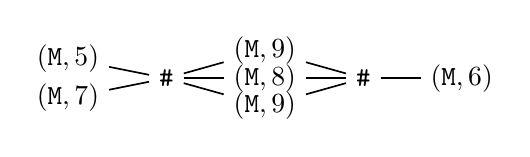
\begin{tikzpicture}[-, >=to, auto, node distance=1.25cm, semithick, transform shape]
\node (M1) {};
\node (T1) [above of=M1, node distance=0.25cm] {$(\tg M,5)$};
\node (B1) [below of=M1, node distance=0.25cm] {$(\tg M,7)$};
\node (M2) [right of=M1] {$\tg\#$};
\node (M3) [right of=M2] {$(\tg M,8)$};
\node (T3) [above of=M3, node distance=0.35cm] {$(\tg M,9)$};
\node (B3) [below of=M3, node distance=0.35cm] {$(\tg M,9)$};
\node (M4) [right of=M3] {$\tg\#$};
\node (M5) [right of=M4] {$(\tg M,6)$};
%
\path (T1) edge (M2);
\path (B1) edge (M2);
\path (M2) edge (T3);
\path (M2) edge (M3);
\path (M2) edge (B3);
\path (T3) edge (M4);
\path (M3) edge (M4);
\path (B3) edge (M4);
\path (M4) edge (M5);
\end{tikzpicture}
}%
\vspace{-1ex}
\newline
where a line from left to right indicates that the item on the right must occur after the item on the left. The end-of-second markers $\tg\#$ separate multisets of natural numbers. So, the set of data traces of $X$ has an isomorphic representation as the set $\text{Bag}(\mathbb{N})^+$ of nonempty sequences of multisets of natural numbers. In particular, the empty sequence $\epsilon$ is represented as $\emptyset$ and the single-element sequence $\tg\#$ is represented as $\emptyset \; \emptyset$.
\end{example}

Key properties described in the data trace types work bear close resemblance to the properties in \Cref{sec:operator-properties}.
The notion of a \emph{data-string transduction} is similar to a monotone operator; it is a monotone function $f: A^* \to B^*$. (So to be precise, a data-string transduction is a monotone functional operator.)
Going further, the definition of \emph{consistency}, which describes when a data-string transduction gives rise to a data-trace type, bears close resemblance to type safety and determinism of operators:

\begin{definition}[Consistency]
Let $X = (A,D)$ and $Y = (B,E)$ be data-trace types. We say that a data-string transduction $f: A^* \to B^*$
is \emph{$(X,Y)$-consistent} if $u \equiv_D v$ implies that $\bar{f}(u) \equiv_{E} \bar{f}(v)$ for all $u, v \in A^*$.
\end{definition}

\chapter{Compositionality}
\label{cha:composition}
\headerblock{%
  \headerquote{The meaning of a compound expression is a function of the meanings of its parts and of the syntactic rule by which they are combined.}{Barbara Partee, 1984~\cite{partee1984compositionality}, as formulated in~\cite{partee1990mathematical}}
  % Partee 1984: The meaning of an expression is a function of the meanings of its parts and of the way they are syntactically combined
  % Partee et. al. 1990: The meaning of a compound expression is a function of the meanings of its parts and of the syntactic rule by which they are combined
}

In this section, we define \emph{SPS-transformers} (SPSTs), a programming language for computations over series-parallel streams.
If synchronization schemas are provided as types for the input and output streams of a computation,
then an SPST is a (type-safe and deterministic) function from input batches to output batches, which respects the structure given by the types. This material was originally presented in~\citeMain{pods21} (some of it was delegated to the appendix).

The primary goal of SPSTs is to be \emph{compositional}: they allow for defining operators over a stream in a compositional way with respect to the type of that stream.
% This is similar to how events, batches, linearizations, and other relations in \Cref{cha:foundation} are defined compositionally on the structure of the stream via typing rules.
Per the goals of our introduction, every SPST should satisfy a type-safety property.
Formally, it should be a deterministic function from input batches to output batches.
By \Cref{thm:type-safe-and-deterministic-converse} this implies that a corresponding \emph{operator}, a low-level function from lists of input to lists of output, can be defined that is type safe and deterministic
in a more realistic event-by-event processing sense.
We will define the semantics of an SPST inductively on the input structure; the typing judgments for this semantics in each case demonstrate type-safety.

An interesting aspect of the material in this section -- which we have found helpful as a way to think about future work in this space -- is the approach to achieve incremental processing by distinguishing \emph{open} and \emph{closed} semantics. For each transformer, the open semantics represents a monotonically-increasing function from input streams to output streams, i.e. an operator that satisfies \emph{monotonicity}. The \emph{closed} semantics represents the semantics after the input stream is terminated, so that the stream operator may produce some final output that is not incremental.
For example, using this distinction, the function \textsc{Sum} described in \Cref{fig:operator-properties-examples} can be represented as a function which produces no output in its open semantics, but produces the total sum in its closed semantics.
We describe this distinction further in \Cref{45:sec:design-goals}.

\section{Notational Differences}

The material in this section uses the definitions, notation, and terminology from~\citeMain{pods21},
rather than those from \Cref{cha:foundation}.
Stream types are called \emph{synchronization schemas},
and batches are called \emph{series-parallel streams}, or \textbf{sps} (SPS)
for short.
In synchronization schemas, instead of base types $T$, there are sets of headers $\mathcal{H}$, representing the possible tuples that might occur for an event
(See \Cref{sec:historical}).
So if $T = \mathcal{H} = (H_1, H_2, H_3)$ for example, then $H_1$, $H_2$, and $H_3$ are tuple types and the events of type $T$ are either tuples of type $H_1$, or tuples of type $H_2$, or tuples of type $H_3$.
It uses the notation $\preceq$ for stream prefix.
This is defined using concatenation:
for batches $b_1$ and $b_2$, we say $b_1 \preceq b_2$ if there is some $b_1'$ such that $b_2 = b_1 \circ b_1'$.

\section{Design Goals}
\label{45:sec:design-goals}

In addition to satisfying \textbf{monotonicity}, \textbf{type safety}, and \textbf{determinism} as already discussed,
SPSTs should satisfy the following additional design goals.
First, they should respect the \textbf{parallelism}
in the input and output: parallel input events should be processed in parallel,
and parallel input threads should produce parallel output events.
% Thus, SPS transformers should be guaranteed to respect and maintain that parallelism.
For example, given an input which is two streams in parallel, the computation should be written in such a way that the two streams are processed separately, and outputs corresponding to them should be unordered.
Second,
to allow for the specification of potentially complex computations, we additionally want our language to be \textbf{compositional}: it should be natural to construct a computation by combining sub-computations.
For example, processing a stream of the hierarchical type $\hier{\mathcal{H}}{S}$
should be definable, both syntactically and semantically, in terms of
existing computations defined over sub-streams of type $S$.
Finally, any computation in our language should be \textbf{incremental} (or \emph{streamable}): it should process the input in one pass, producing output incrementally.

To satisfy these design goals, we make the following technical choices.
First, to satisfy the parallelism goal, we define SPSTs to have SPSs as input and output rather than sequential objects.
The input being an SPS allows us to specify the computation to exploit parallelism,
and the output being an SPS requires that we respect parallelism when producing output events.

To understand  the challenges in defining the semantics due to the interplay between streamability and compositionality, consider a transformer $P$ processing
hierarchical streams of type  $S=\hier{\mathcal{H}}{S'}$ that we would like
define in terms of a transformer $P'$ processing streams of type $S'$.
Consider an input stream $t=[\spsemp, d, t']$ of type $S$ for an $\mathcal{H}$-tuple $d$ and
stream $t'$ of type $S'$. Suppose we want to extend the input stream $t$ with
a tuple $d'$. If the type of $d'$ is one of the headers appearing in $S'$, then
it really extends the sub-stream $t'$, and should be processed by the transformer $P'$.
For incrementality, we want to make sure that, while processing $d'$, $P'$ extends the output stream only
by adding new items. Formally, this means that the output of $P'$ on the input
stream $t'$ should be a prefix of its output on the stream $t'\circ d$.
With this motivation, we define such a semantics, which we call \emph{open} semantics,
for transformers as functions from input to output streams, and ensure that it is \emph{monotonic}
 with respect to prefix ordering
(see Theorem~\ref{45:thm:spst-monotonicity}).
But now suppose that the item $d'$ is an ${\mathcal H}$-tuple
that acts as a synchronization marker for the events in the sub-stream $t'$.
Then to process it, the transformer $P'$ should return, and let the top-level
transformer $P$ process the item $d'$.
During this return, the transformer $P'$ can do additional computation and produce
additional output items even though the stream it has processed is still $t'$.
This is a typical case when $S'$ corresponds to key-based partitioning,
and the arrival of the synchronization marker $d'$ triggers the reduce operation
that aggregates the results of the computations of the key-indexed sub-streams of $t'$.
This though requires us to define another semantics of the transformer $P'$ on
the input stream $t'$ that extends the open semantics and includes the results
of the computation upon return. We call it \emph{closed} semantics to indicate
that it is applicable when the current stream  is being closed.
Note that the result of computation of $P$ on the stream $[\spsemp, d,t',d', \spsemp]$ can be
described by relying on the closed semantics of $P'$ on the stream $t'$.
In terms of existing work on punctuation,
the closed semantics can be thought of as the stream output on
a stream terminated by an \emph{end-of-stream} marker.

Finally, an SPST is a function on pairs:
it takes an initial value and an input
SPS to a final value and an output SPS.
We need this for compositionality: without the initial value as input, an SPS-transformer
on a sub-stream of the input could not be initialized based on the surrounding context.
Similarly, the final value (separate from the series of output items produced) can be
used to describe a summary of the input stream to be used in the surrounding context
when the computation finishes.

%this means that if the input stream is extended (additional items added that are later than all existing items), the output must also be an extension of the previous output. However, to satisfy compositionality, sometimes for an \emph{intermediate} result we don't need it to be monotonic in order for the overall computation to be monotonic. To allow for this, formally, we distinguish between two semantics: an monotonic \emph{open} semantics, which takes an input stream which is thought of as being unfinished (may receive more items), and produces an output stream; and a \emph{closed} semantics, which takes an input stream which is thought of as being finished (may not receive more items), and produces a final output, which need not be monotonic. The open semantics will be a prefix of the closed semantics. The final value of the computation is naturally a part of the closed semantics, but not the open semantics.

We summarize all of these choices in the following definition of the \emph{interface}
for an SPST.
We also define subtyping for the interface, where the output is relaxed.
Each of the language constructs will then implement this interface.
In \Cref{45:ssec:spst-example}, we give an extended example
to illustrate the formal definitions in this section.

\begin{definition}[SPS-transformer interface]
An SPS-transformer (SPST) $P$
has:
\begin{itemize}
\item A \emph{type} denoted $(X, S, X', S')$,
where
$X$ is the type for the initialization value,
$S$ is an input synchronization schema,
$X'$ is a type for the final return value,
and $S'$ is an output synchronization schema.
We write $P: (X, S, X', S')$.

\item An \emph{open semantics} denoted $\spstsemO{x}{t}{P} = t'$,
where $x: X$ is the initial value, $t: S$ is the input SPS,
and $t': S'$ is the incrementally produced output SPS.

\item A \emph{closed semantics} denoted $\spstsemC{x}{t}{P} = (x', t')$,
where $x': X'$ is the initial value, $t: S$ is the input SPS,
$x': X'$ is the final value, and $t': S'$ is the output SPS.
We additionally enforce that the open semantics is a prefix
of the closed semantics:
$\spstsemO{x}{t}{P} \prefix t'$.

\end{itemize}
\end{definition}

\begin{definition}
\label{45:def:spst-subtyping}
If $S'' \lesssim S'$ (Definition~\ref{def:stream-relaxation}),
then $(X, S, X', S'')$ is a \emph{subtype} of $(X, S, X', S')$.
If $P: (X, S, X', S')$
then we also write $P: (X, S, X', S'')$.
The open and closed semantics are derived as the unique output stream
given by Proposition~\ref{45:prop:schema-relaxation-flattening}.

\end{definition}

\noindent
In the remainder of the section,
we give one language construct corresponding to each constructor of the input series-parallel stream.
Some additional notation:
for a set of headers $\mathcal{H}$,
we write $\tup(\mathcal{H})$ for the set of tuples $x: \mathcal{H}$.
For a synchronization schema $S$,
we write $\sps(S)$ for the set of SPSs $t: S$.
We write $\bag(X)$ for the set of bags (multisets) of items of type $X$.
% \str
% \caleb{\bag(X) is currently only used in the partition-by case. I wonder if we can replace
% it with sps(Bag(..)) for some appropriate schema.}

% \kk{Rajeev suggestions:}
% \kk{Make relational SPST a special case and don't even define syntax.}
% \kk{Closed semantics should be renamed and only return the extension of the sps and the final value. (Maybe)}

\section{Syntax and Semantics}

\subsection{Relational SPST}

We start with the relational SPST, which represents a standard relational operator that can be used to process a bag of items, producing another bag of items.
Relational operators are well studied and are commonly defined using SQL
and its extensions.
Our design choice here is to not impose a particular relational base language
or SQL variant;
instead,
the relational operator is given as two \emph{black-box} functions,
which define the open and closed semantics,
respectively.
We only require that these are functions on bags (i.e., independent of the input order),
and that the open semantics is monotone and a prefix
of the closed semantics.
% For example, in an implementation, these black-box functions might then be defined
% by SQL or any of its extensions.
% In practice, relational operators often have streaming implementations that can process their inputs incrementally, but their output is still guaranteed to be the same regardless of the input order.
% Importantly, relational operators are not affected by the order in which their input arrives and produce the same result for any order of inputs.

\begin{definition}[Relational SPST]
A relational SPST
\[P : (X, \relleaf{\mathcal{H}}, X', \relleaf{\mathcal{H}'})\]
consists of two fields:
\begin{align*}
\spstfield{P}{open} &: X \times \sps(\relleaf{\mathcal{H}}) \to \sps(\relleaf{\mathcal{H}'}) \\
\text{and} \quad
\spstfield{P}{closed} &: X \times \sps(\relleaf{\mathcal{H}}) \to X' \times \sps(\relleaf{\mathcal{H}'}).
\end{align*}
such that
(1) $\spstfield{P}{open}$ is \emph{monotone}:
if $r_1 \prefix r_2$, then $\spstfield{P}{open}(x, r_1) \prefix \spstfield{P}{open}(x, r_2)$;
and
(2) $\spstfield{P}{open}$ is a prefix of $\spstfield{P}{closed}$:
if $\spstfield{P}{closed}(x, r)$ $= (x', r')$
then $\spstfield{P}{open}(x, r) \prefix r'$.
The semantics of $P$ is defined as
$\spstsemO{x}{r}{P} = \spstfield{P}{open}(x, r)$
and $\spstsemC{x}{r}{P} = \spstfield{P}{closed}(x, r)$.

\end{definition}

\subsection{Parallel SPST}

We now define the inductive SPSTs.
An SPST processing inputs of type
$\parcomp{S_1}{S_2}$ is composed of two SPSTs running in parallel independently.
The question here is, can the components SPSTs produce tuples of the same type?
The answer is yes, provided such tuples, since they get produced independently,
are summarized using a schema $\relleaf{\mathcal{O}}$,
where $\mathcal{O}$ is a set of output headers.
So the output schema for the parallel SPST
will be $\parthree{S_1'}{S_2'}{\relleaf{\mathcal{O}}}$.
%The semantic behavior of a parallel SPST respects the parallelism in the input: it %first initializes the states of the two sub-SPSTs, it then runs the two sub-SPSTs in parallel.
% For the closed semantics, we also can process the two final values of the sub-SPSTs.

\begin{definition}[Parallel SPST]
Let $S_1, S_2, S_1', S_2'$ be schemas.
A parallel SPST
\[
P : (X, \parcomp{S_1}{S_2}, X', \parthree{S_1'}{S_2'}{\relleaf{\mathcal{O}'}})
\]
consists of internal types $X_1, X_2, X_1', X_2'$ and
four fields:
\begin{align*}
\spstfield{P}{left} &: (X_1, S_1, X_1', \parcomp{S_1'}{\relleaf{\mathcal{O}'}}), \\
\spstfield{P}{right} &: (X_2, S_2, X_2', \parcomp{S_2'}{\relleaf{\mathcal{O}'}}), \\
\spstfield{P}{init} &: X \to X_1 \times X_2,
\quad \text{and} \quad
\spstfield{P}{fin} : X_1' \times X_2' \to X'.
\end{align*}
The semantics of $P$ is as follows: if we have that
$\spstfield{P}{init}(x) = (x_1, x_2)$,
$\spstsemO{x_1}{t_1}{\spstfield{P}{left}} = \spspar{t_1'}{r_1'}$,
and
$\spstsemO{x_2}{t_2}{\spstfield{P}{right}} = \spspar{t_2'}{r_2'}$,
where $r_1', r_2': \relleaf{\mathcal{O}'}$,
and
additionally $\spstsemC{x_1}{t_1}{\spstfield{P}{left}} = (x_1', \spspar{t_1''}{r_1''})$
and
$\spstsemC{x_2}{t_2}{\spstfield{P}{right}} = (x_2', \spspar{t_2''}{r_2''})$,
then
\begin{align*}
\spstsemO{x_1}{t_1}{P}
    &= \spspar{\spspar{t_1'}{t_2'}}{r_1' \cup r_2'} \\
\spstsemC{x_1}{t_1}{P}
    &= ( \spstfield{P}{fin}(x_1', x_2'),
         \spspar{\spspar{t_1''}{t_2''}}{r_1'' \cup r_2''} ).
\end{align*}
\end{definition}

\subsection{Hierarchical SPST}

When the input schema is $S=\hier{\mathcal{H}}{S_1}$, we want to
define the corresponding SPST $P$ parameterized by a sub-SPST from
$S_1$ to $S'_1$.
The SPST $P$ maintains its own state that gets updated sequentially
whenever any $\mathcal{H}$-tuple is processed,
is passed to the sub-SPST when called, and is updated when the sub-SPST returns.
The output schema of $P$ has the same structure as the input:
it is divided into synchronizing events and non-synchronizing events.
On input synchronization events, any output tuple may be produced,
including a synchronization event; but on input sub-stream events, it would be incorrect
to produce an output synchronizing event, as this would not be produced in a consistent order.
% Thus, we define a hierarchical SPST from input schema
% $S = \hier{\mathcal{H}}{S_1}$
% to output schema $S' = \hier{\mathcal{H}'}{S_1'}$.
% Recall that it is guaranteed that the input stream alternates between substreams
% $t_i: S_1$
% and synchronization events $d_i: \mathcal{H}$.
%The SPST is parameterized by  it uses a \emph{call} and \emph{return} function to pass state to and from the sub-SPST.
% the sub-SPST and collect
% and an update function, which is called on each synchronization event $d_i$.
% Both the update function and the final function (at the end of the stream)
% may produce any output event, i.e. any SPS in $S'$.
% Finally, the SPST has \emph{call}
% and \emph{return} functions to initialize and finalize the sub-SPST
% computation: these are important as they are
% where the initial and final value types in SPSTs
% come into play in the modular composition of SPSTs.
The distinction between closed and open
semantics plays a key role here:
%in contrast to the semantics of the other SPSTs, where the open semantics is only defined with respect to open semantics of the sub-SPSTs.
synchronizing events, when processed by $P$, ``close'' the computation of the sub-SPST.
%Thus, the closed semantics is used for the sub-SPST,
%not the open semantics, except on the final sub-stream.
% i.e. in the open semantics,
% for $t_i$ terminated by a $d_i$ event,
% we use the closed semantics on the sub-SPST;
% but for the final sub-stream $t_m$,
% we use the open semantics for $t_m$
% as, intuitively, this stream
% may still receive more items.
To formalize this inductively,
we introduce an auxiliary semantics $\spstsemI{y}{t}{P}$
where the output is an internal state (rather than a final value),
and in which the input stream ends with a $d_i$ event,
i.e., the final $t_i$ is $\spsemp{}$.

\begin{definition}[Hierarchical SPST]
Let $S_1$ and $S_1'$ be schemas, and $\mathcal{H}$ and $\mathcal{H}'$
be a set of input and output headers, respectively.
Let $S' = \hier{\mathcal{H}'}{S_1'}$.
A hierarchical SPST
\[
P : (X, \hier{\mathcal{H}}{S_1}, X', \hier{\mathcal{H}'}{S_1'})
\]
consists of internal types $X_1, X_1', Y$ and
six fields:
\begin{alignat*}{3}
\spstfield{P}{sub} &: (X_1, S_1, X_1', S_1'),
    \hspace{-1em} \\
\spstfield{P}{update} &: Y \times \tup(\mathcal{H}) \to Y \times \sps(S'),
    \hspace{-8em} \\
\spstfield{P}{call} &: Y \to X_1,
    &\spstfield{P}{return} &: Y \times X_1' \to Y, \\
\spstfield{P}{init} &: X \to Y,
    &\text{and} \quad \spstfield{P}{fin} &: Y \to X' \times \sps(S').
\end{alignat*}

The auxiliary semantics of $P$ is denoted
$\spstsemI{y}{t}{P} = (y', t')$, where $y, y': Y$,
and defined inductively
\emph{only} for $t$
of the form $[t_0, d_1, t_1, \ldots, d_m, \spsemp{}]$.
For the base case, $\spstsemI{y}{\spsemp{}}{P} = (y, \spsemp{})$.
Then inductively, if
$\spstsemI{y}{t}{P} = (y', t')$,
$t_1: S_1$, and
$d: \mathcal{H}$,
and if we have
$\spstfield{P}{call}(y') = x_1$,
$\spstsemC{x_1}{t_1}{\spstfield{P}{sub}} = (x_1', t_1')$,
$\spstfield{P}{return}(y', x_1') = y''$,
and $\spstfield{P}{update}(y'', d) = (y''', t'')$,
then
$\spstsemI{y}{t \circ \spsseq{t_1, d, \spsemp}}{P} = (y''', t' \circ t_1' \circ t'')$.
Given the auxiliary semantics, we define the semantics
of $P$ on a trace decomposed as $t \circ \spsseq{t_1}$,
where the last list item of $t$ ia an empty sub-trace.
Let
$\spstfield{P}{init}(x) = y$,
$\spstsemI{y}{t}{P} = (y', t')$,
and $\spstfield{P}{call}(y') = x_1$.
Additionally, let
$\spstsemC{x_1}{t_1}{\spstfield{P}{sub}} = (x_1', t_1')$,
$\spstfield{P}{return}(y', x_1') = y''$,
and $\spstfield{P}{fin}(y'') = (x', t'')$.
Then:
\begin{align*}
\spstsemO{x}{t}{P}
    &= t' \circ \spstsemO{x_1}{t_1}{\spstfield{P}{sub}} \\
\spstsemC{x}{t}{P}
    &= (x', t' \circ t_1' \circ t'').
\end{align*}
\end{definition}

% \subsection{Sequential SPST}

% Recall that $\seqleaf{\mathcal{H}}$ is a useful special case of hierarchical synchronization schemas
% that denotes simple sequences, i.e. it is the schema $\hier{\mathcal{H}}{\relleaf{\varnothing}}$.
% We define an SPST for this case for convenience,
% a special case of SPST for the hierarchical case.
% This SPST transform a sequence of tuples and an initial state to an output sequence of tuples and a final state.
% Sequential SPSTs are used for any computation that depends on the order of the input tuples, such as a linear interpolation, or string recognition.

% \begin{definition}[Sequential SPST]
% A sequential SPST
% \[
% P : (X, \seqleaf{\mathcal{H}}, X',  \seqleaf{\mathcal{H'}})
% \]
% consists of four fields: an internal state type $Y$, an initialization function $\spstfield{P}{init} : X \to Y$, a sequential update function $\spstfield{P}{update} : Y \times \tup(\mathcal{H}) \to Y \times (\mathcal{H'})^{*}$, and a finalization function $\spstfield{P}{fin} : Y \to X'$.
% Semantically, it functions the same as the following hierarchical SPST $P'$:
% $P'$ has the same internal state type $Y$;
% the same $\spstfield{P'}{init}$, $\spstfield{P'}{update}$, and $\spstfield{P'}{fin}$;
% a child SPST $\spstfield{P'}{sub}: (Y, \relleaf{\varnothing}, Y, \relleaf{\varnothing})$
% which is the trivial relational operator
% i.e. $\spstfield{(\spstfield{P'}{sub})}{op}(y, ()) = (y, ())$,
% and the identity call and return functions
% $\spstfield{P'}{call}: Y \to Y$ and $\spstfield{P'}{return}: Y \to Y$.
% \end{definition}

\subsection{Partitioned SPST}

Finally, we define SPST for the partition-by case.
The idea here is analogous to the parallel composition $\parcomp{S_1}{S_2}$ case: each sub-stream corresponding to a different key value may produce output corresponding to that key value, \emph{or} produce output corresponding to a common bag of tuples $\mathcal{O}'$.
The partitioned SPST initializes the state of $\spstfield{P}{sub}$ for each key with a nonempty SPS and runs the child SPST for each (non-empty) key in parallel.
We additionally need an aggregation stage (applicable to the closed semantics only),
in which we combine all of the partitioned states
using a black-box relational operator $\spstfield{P}{agg}$,
similar to what was done in the relational SPST base case.
% This aggregation function (or reducer) also may produce outputs in $\mathcal{O}'$ if desired.

\begin{definition}[Partitioned SPST]
Let $S = \keyby{K}{S_1}$ and $S' = \keyby{K}{S_1'}$ be schemas,
and $\mathcal{O}'$ a set of headers.
A partitioned SPST
\[
P : (X, \keyby{K}{S_1}, X', \parcomp{\keyby{K}{S_1'}}{\relleaf{\mathcal{O}'}}
\]
consists of internal types $X_1, X_1'$ and three fields:
\begin{align*}
\spstfield{P}{sub} &: (X_1, S_1, X_1', \parcomp{S_1'}{\relleaf{\mathcal{O}'}}), \\
\spstfield{P}{init} &: X \times \tup(K) \to X_1, \\
\text{and} \quad
\spstfield{P}{agg} &: X \times \bag((\tup(K) \times X_1') \to X' \times \bag(\tup(\mathcal{O}')).
\end{align*}

For the semantics,
suppose $t = \spsbag{\keyed{v_1}{t_1}, \ldots, \keyed{v_m}{t_m}}$,
and for $i = 1, \ldots, m$,
$\spstfield{P}{init}(x, v_i) = x_i$,
$\spstsemC{x_i}{t_i}{\spstfield{P}{sub}} = (x_i', \spspar{t_i'}{r_i'})$,
$\spstfield{P}{agg}(x, \{(v_1, x_1), \ldots, (v_m, x_m)\}) = (x', r_0')$,
and
$\spstsemO{x_i}{t_i}{\spstfield{P}{sub}} = \spspar{t_i''}{r_i''}$.
Then
\begin{align*}
    \spstsemC{x}{t}{P}
    &= (x', \spspar{ \spsbag{\keyed{v_1}{t_1'}, \ldots, \keyed{v_m}{t_m'}}}{r_0' \cup r_1' \cup \cdots \cup r_m'}
    \\
    \spstsemO{x}{t}{P}
    &= \spspar{\spsbag{\keyed{v_1}{t_1''}, \ldots, \keyed{v_m}{t_m''}}}{r_1'' \cup \cdots \cup r_m''}.
    \quad
\end{align*}
\end{definition}

\section{Examples}
\label{45:ssec:spst-example}

To illustrate the definition of the various SPST constructs,
we continue the example schema from \Cref{45:fig:example-schema} as the input type.
For the output, suppose we want to produce two kinds of events: \code{EndOfHour},
representing end-of-hour summaries, and \code{Outlier}, representing
outlier events that should be logged for further investigation.
We describe building an SPST with this input and output,
building it bottom-up from the structure of the input schema.

We begin with an example of a relational SPST.
We describe the transformation on \code{RideCompleted}
events which computes the sum of the costs of all completed hours.
The interface of this SPST is $
P_1: ((), \relleaf{ \code{RideCompleted} }, \code{float}, \emptyset)$.
As it consumes a bag of \code{RideCompleted} events,
it does not produce any output tuples, but instead we aggregate the sum of the return
costs as a single \code{float}.
For this relational base case,
the computation can be written using an aggregator in a base relational language
such as SQL.
Formally, in our framework $P_1$ is defined by two black-box functions:
$\spstfield{P}{open}((), r) = \spsemp$
and $\spstfield{P}{closed}((), \spsbag{x_1, \ldots, x_m}) = (x_1 + \cdots + x_m, \spsemp)$.
The former component $\spstfield{P}{open}$
indicates that in this case no events are produced incrementally
(as the input stream is processed).
The latter component $\spstfield{P}{closed}$
indicates that the final result of the computation (after the entire input stream is seen)
is the sum of all tuples in the input relation.

Next, we describe a simple sequential SPST
which processes a linear sequence of \code{GPS}
events.
Recall that $\seqleaf{\mathcal{H}}$ is a useful special case of hierarchical synchronization schemas
that denote simple sequences, i.e. it is the schema $\hier{\mathcal{H}}{\relleaf{\varnothing}}$.
Suppose we want to compute the distance traveled for a specific taxi given its \code{GPS} tuples;
additionally,
suppose we want to produce as output \emph{outlier} \code{GPS}
tuples, rather than including them in the aggregation.
\[
P_2: ((),
    \seqleaf{ \code{GPS} },
    \code{float},
    \seqleaf{ \code{Outlier} })
\]


$P_2$ keeps the last known location for the taxi and the current distance traveled as its state, and each time it processes a new \code{GPS} tuple, it updates both.
Additionally, if the last known location is too far from the current one
($> 1$ below)
instead of updating state it produces the tuple as output.
\begin{align*}
\spstfield{P_2}{update}((\bot, 0), gps)
    &= (( gps.loc, 0), \spsemp) \\
\spstfield{P_2}{update}((loc, d), gps)
    &= (( gps.loc, d + dist(gps.loc, loc)) \\
    &\quad\quad\text{if } dist(gps.loc, loc) \le 1 \\
\spstfield{P_2}{update}((loc, d), gps)
    &= (( loc, d), \code{Outlier}(loc)) \\
    &\quad\quad\text{otherwise}
\end{align*}

% \begin{alignat*}{3}
% & \spstfield{P_2}{update}((\bot, 0), gps) && = (( && gps.loc, 0), \spsemp) \\
% & \spstfield{P_2}{update}((loc, d), gps) && = (( && gps.loc, d + \\
% & && && dist(gps.loc, loc)), \spsemp) \\
% & \spstfield{P_2}{update}((loc, d), gps) && = (( && loc, d), \code{Outlier}(loc))
% \end{alignat*}
Because this is a sequential base case
(a special case of hierarchical),
$\spstfield{P_2}{sub}$, $\spstfield{P_2}{call}$, and $\spstfield{P_2}{return}$
are trivial with no effect on the state.
Finally, $\spstfield{P_2}{init}(()) = (\bot, 0)$,
and $\spstfield{P_2}{fin}(loc, d) = (d, \spsemp)$.

Next, we define the partitioned SPST that computes the total distance traveled by all taxis (according to the taxi example described in \Cref{45:fig:example-schema}).
The interface of the SPST is
\[
P_3:
((),
    \keyby{\code{taxiID}}{\seqleaf{ \code{GPS} }},
    \code{float},
    \relleaf{\code{Outlier}})
\]
since it returns the total distance traveled by all taxis in miles.
The child SPST is $P_2$, i.e., $\spstfield{P_3}{sub} = P_2$,
However, notice that instead of a sequential output, here the output outliers
are a bag: this is because there are multiple keys (taxi IDs),
so different key outputs may be unordered.
Implicitly, we are relaxing the output of $P_2$ to be a bag instead of a sequence:
this illustrates SPST \emph{subtyping} (Definition~\ref{45:def:spst-subtyping}),
in which ordered output events may be reinterpreted as unordered.
The interface of our sequential SPST is now
$P_2: \seqleaf{ \code{GPS} }, \code{float}, \seqleaf{ \code{Outlier} })$.
To fit the SPST definition exactly,
we would additionally relax to $\parcomp{\varnothing}{\seqleaf{ \code{Outlier} }}$
(to allow both keyed and bag outputs),
but we leave this off for presentation;
it is just another application of subtyping since the schemas are equivalent.
To complete the definition of $P_3$,
the aggregation
produces a sum of the distances:
\[
\spstfield{P_3}{agg}(\_, ds) = (sum( \{ d \mid (\_, d) \in ds \} ), \spsemp{})
\]
and $\spstfield{P_3}{init}$ initializes all child SPSTs with the unit value.

At this point, we have a partitioned SPST $P_3$ for processing
the key-partitioned \code{GPS} stream,
and we have a relational SPST $P_1$ for processing the
\code{RideCompleted} events.
In order to combine these into
an overall query
which also processes the \code{EndOfHour}
synchronizing events,
we first need to combine these two streams in parallel.
We define an SPST $P_4$ which
divides the aggregate cost by the aggregate distance.
Let $S_1 = \keyby{\code{taxiID}}{\seqleaf{ \code{GPS} }}$
and $S_2 = \relleaf{ \code{RideCompleted} }$.
Then the interface of $P_4$ is
\[
P_4: ((), \parcomp{S_1}{S_2}, \code{float}, \relleaf{ \code{Outlier} }).
\]
The SPST calls the underlying SPSTs $P_1$ and $P_3$: $\spstfield{P_4}{left} = P_3$ and $\spstfield{P_4}{right} = P_1$, which return the total distance covered by all taxis and the total cost of all completed rides in that hour,
and then simply divides to return the \code{float} ride cost per traveled mile, i.e., $\spstfield{P}{fin}(dist, cost) = cost / dist$.

Notice that the average value in $P_4$
is only computed on finalization (after the entire stream is processed).
In order to produce the same averages in a streaming manner,
we need \emph{synchronization events},
and this leads us to our final step:
we complete the input schema in Figure~\ref{45:fig:example-schema}
and the example by constructing a hierarchical schema
which also processes
the \code{EndOfHour} synchronization events.
The schema $P_5$ which outputs the cost per distance traveled
at the end of each hour
has the following interface:
\begin{align*}
P_5: (
    &(), \hier{ \code{EndOfHour} }{ \parcomp{S_1}{S_2} }, \\
    &(), \hier{ \code{CostPerMile} }{ \relleaf{\code{Outlier}} }
)
\end{align*}
The SPST calls the underlying SPST $P_4$, i.e., $\spstfield{P_5}{sub} = P_4$,  which returns the cost per mile in the last hour as a \code{float}.
$P_4$ also produces the \code{Outlier} output events.
The internal state $Y$ is the cost per mile
from the last substream.
The function $\spstfield{P_5}{call}$
does not pass anything to $P_4$,
but $\spstfield{P_5}{return}$ does consume the final \code{float}
and stores it in the state.
Then $P_5$ simply outputs the \code{float} when processing an \code{EndOfHour} tuple:
\[
\spstfield{P_5}{update}(cpm, \_) = (cpm, \code{CostPerMile}(cpm)).
\]

\section{Monotonicity}
\label{45:sec:theorems}

The following is the major technical result of this chapter: for any SPST, the open semantics is monotone in the prefix relation on partially ordered streams.
This ensures that event-by-event incremental processing is possible, though it does not define the event-by-event logic explicitly.

\begin{theorem}
\label{45:thm:spst-monotonicity}
Let $P: (X, S, X', S')$ be an SPST.
Then $P$ is monotone in the following sense:
for any $x: X$ and $t, u: S$,
if $t\prefix u$,
then $\spstsemO{x}{t}{P} \prefix \spstsemO{x}{u}{P}$.
% for any $x: X$ and $t, u: S$,
% there exists $u'$ such that
% $\spstsemO{x}{t \circ u}{P} = \spstsemO{x}{t}{P} \circ u'$.
\end{theorem}
\begin{proof}
  The proof is by induction on $P$.
  We strengthen the hypothesis to additionally show that
  the open semantics is a prefix of the closed semantics:
  if $\spstsemC{x}{t}{P} = (x', t')$ then $\spstsemO{x}{t}{P} \prefix t'$.
  In addition to the definition of concatenation $\circ$
  and prefix $\prefix$,
  we use that $\prefix$ is a partial order
  (Proposition~\ref{45:prop:sps-concat-properties}).
  One of the inductive cases is subtyping
  as given by Definition~\ref{45:def:spst-subtyping}.
  % we use the following derived facts about $\circ$ which can be shown using the definition.
  % (1) Identity: for any SPS $t$, $t \circ \spsemp = \spsemp \circ t = t$,
  % where $\spsemp$ is the empty SPS for that case (empty bag, empty sequence,
  % or empty key-partitioned map).
  % (2) Associativity: $(t_1 \circ t_2) \circ t_3 = t_1 \circ (t_2 \circ t_3)$.
  \begin{itemize}
  \item In the relational case,
  $\spstfield{P}{open}$ is monotonic and a subset relation
  of $\spstfield{P}{closed}$ by assumption.
  \item In the parallel case,
  let $t = \spspar{t_1}{t_2}$ and $u = \spspar{u_1}{u_2}$,
  and suppose that we have
  $\spstsemO{x_1}{t_1}{\spstfield{P}{left}} = t_1'$,
  $\spstsemO{x_1}{u_1}{\spstfield{P}{left}} = u_1'$,
  $\spstsemO{x_2}{t_2}{\spstfield{P}{right}} = t_2'$, and
  $\spstsemO{x_2}{u_2}{\spstfield{P}{right}} = u_2'$.
  Applying the inductive hypothesis, what we need to
  show is that if $t_1' \prefix u_1'$ and $t_2' \prefix u_2'$,
  then
  $\spspar{t_1'}{t_2'} \prefix \spspar{u_1'}{u_2'}$.
  This follows by unfolding the definitions of prefix and underlying concatenation,
  which works component-wise on $\spspar{t_1'}{t_2'}$.
  The same reasoning applies to
  comparing the open and closed semantics.

  \item
  In the hierarchical case,
  our first step is to prove that the auxiliary semantics
  is monotonic.
  For this, we only consider when $t$ and $u$ each end in an empty sub-trace
  $t_m = \spsemp$ and $u_m = \spsemp$.
  This then follows by induction on the trace directly
  since the output is a sequence and produced one item at a time
  from the closed semantics of the sub-SPST,
  using transitivity of $\prefix$.
  Next for the general case,
  we observe the following:
  for any trace ending in an empty subtrace $t$,
  and any subtraces $t_1, u_1$ with $t_1 \prefix u_1$,
  the auxiliary semantics on $t$
  is a prefix of the open semantics on $t \circ [t_1]$
  (by definition),
  which is a prefix of the open semantics on $t \circ [u_1]$
  (by IH),
  which is a prefix of the auxiliary semantics on $t$
  concatenated with closed sub-SPST semantics on $u_1$
  (by definition, IH, and associativity of concatenation),
  which is a prefix of the auxiliary semantics
  on $t \circ [u_1, d, \spsemp{}]$ for any $d$
  (by definition).
  This chain of prefix relations
  implies the general monotonicity for $t \prefix u$,
  using transitivity of $\prefix$.
  Also the auxiliary semantics on $t$ concatenated with closed sub-SPST
  semantics on $u_1$ is a prefix of
  the closed semantics on $t \circ [u_1]$
  (by definition),
  which gives that the open semantics is a prefix of closed.

  \item
  Next we consider the partition case.
  For the open semantics, $\spstfield{P}{agg}$ does not factor in.
  We consider the output on $t \circ u$ and $t$
  in two parts: first the keyed output, and second the relational
  output.
  % \begin{itemize}
  % \item
  (i)
  For the keyed output, we need to show that the output on
  $t$ is a prefix of the output on $t \circ u$.
  There are three cases here: the key is present in both
  $t$ and $u$, present in only $t$, and present in only $u$.
  If present in both, the prefix relation holds by induction hypothesis.
  If only in $t$, the output on $t$ and on $t \circ u$ are the same
  as these SPS are the same for this particular key value.
  If only in $u$, the output on $t$ does not contain this particular key value,
  and so is a prefix of the output on $t \circ u$
  taking $u'$ to be the output on $u$ for that key.
  % \item
  (ii)
  For the relational output, we consider the set of key values
  in $t$: for each such value, the output on $t$ and on $t \circ u$
  produces a relation.
  We can ignore key values not in $t$ (in $t \circ u$ only) as they
  only extend the output relation for $t \circ u$.
  Now we need to show that the relational output on $t \circ u$
  is a superset of the relational output on $t$ for each of these keys,
  which is true by induction hypothesis.
  % \end{itemize}
  \item
  Finally, we consider the case of subtyping (output schema relaxation).
  This requires careful application of
  Definition 13 from~\citeMain{pods21},
  Proposition~\ref{45:prop:sps-sequence-correspondence}
  and Proposition~\ref{45:prop:schema-relaxation-flattening}.
  Using these we derive the following lemma:
  given a schema, $t' \prefix u'$
  is equivalent to the following statement:
  every flattening of $t'$
  can be extended to a flattening of $u'$,
  and every flattening of $u'$ is equivalent
  to a extension of a flattening of $t'$.

  Given this lemma,
  let $S$ and $S'$ be the input and output schemas,
  and $S'' \lesssim S'$.
  Let $t', u', t'', u''$ be the output schemas for $t$ and $u$:
  the definition of $t''$ and $u''$ is that
  all flattenings of $t'$ are flattenings of $t''$,
  and all flattenings of $u'$ are flattenings of $u''$.
  We also know by IH that $t' \prefix u'$,
  which we interpret in terms of flattenings by the lemma.
  Considering any flattening of $t''$,
  first we know it only contains events in $\headers(S')$
  (because the original schema output was $S'$),
  and we can additionally show it is equivalent under
  $S''$
  to some flattening of $t'$;
  this $t'$ then can be extended to a flattening of $u'$,
  so the flattening of $t''$ can be extended with the same extension
  to a flattening of $u''$,
  which by the lemma implies $t'' \prefix u''$.
  \qedhere{}
  \end{itemize}
\end{proof}

\section{Distribution}
\label{sec:distribution}

\subsection{Motivating Application}
\label{ssec:motivating-application}

\paragraph{Fraud detection}
Suppose there are two types of input events: bank transactions and fraud detection rules
that are used to flag some transactions as fraudulent. Bank
transactions are continuously input in the system with high rate while new
fraud detection rules arrive infrequently. An example of a new rule would
be the addition of a specific account to an index of suspicious accounts.
There is no way to partition inputs while
avoiding cross-partition dependencies since all events (both
transactions and rules) depend on previous rule events. Still, if the
rate of bank transaction events becomes a bottleneck (and fraud
detection rule events happen rarely) it would be beneficial to
parallelize the processing of bank transaction events.

One of the solutions that has been used to achieve data parallelism in
such computations involves extending the dataflow model with a
\emph{broadcast} pattern that allows sending some input events to \emph{all}
parallel shards (and partitioning the rest of the events as usual). An
example execution of the above computation that utilized the broadcast
pattern is shown in \Cref{fig:broadcast-dependencies-vis}. By
broadcasting the fraud detection rule events, a parallel implementation
is achieved without requiring cross-instance communication between the
parallel instances since dependencies are contained in a single
shard. However, as we see below, this solution does not generalize to
more complex dependencies.

\begin{figure}[t]
    \centering
    \begin{subfigure}[t]{0.45\textwidth}
        \centering \footnotesize{}
        \scalebox{0.8}{
        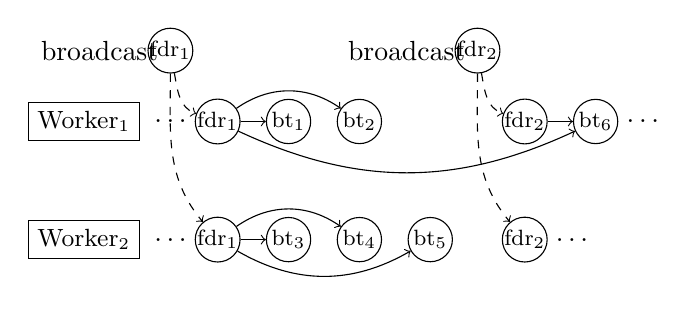
\begin{tikzpicture}[node distance=0.9cm and 0.9cm, on grid]
        %% Top Events
        \node[W] (w1) {$\textrm{Worker}_1$};
        \node[right=1.1 of w1] {$\ldots$};
        \node[B,right=1.7 of w1] (fdr1) {$\textrm{fdr}_1$};
        \node[B,right = of fdr1] (bt1) {$\textrm{bt}_1$};
        \node[B,right = of bt1] (bt2) {$\textrm{bt}_2$};
        \node[B,right=2.1 of bt2] (fdr2) {$\textrm{fdr}_2$};
        \node[B,right = of fdr2] (bt6) {$\textrm{bt}_6$};
        \node[right=0.6 of bt6] {$\ldots$};
        %% Bottom Events
        \node[W,below=1.5 of w1] (w2) {$\textrm{Worker}_2$};
        \node[right=1.1 of w2] {$\ldots$};
        \node[B,right=1.7 of w2] (fdr1') {$\textrm{fdr}_1$};
        \node[B,right = of fdr1'] (bt3) {$\textrm{bt}_3$};
        \node[B,right = of bt3] (bt4) {$\textrm{bt}_4$};
        \node[B,right = of bt4] (bt5) {$\textrm{bt}_5$};
        \node[B,right=1.2 of bt5] (fdr2') {$\textrm{fdr}_2$};
        \node[right=0.6 of fdr2'] {$\ldots$};
        %% Broadcasted events
        \node[B,above left=0.9 and 0.6 of fdr1] (fdr1root) {$\textrm{fdr}_1$};
        \node[left= of fdr1root] (broadcastfdr1) {$\textrm{broadcast}$};
        \draw[dashed,->] (fdr1root) to [out=280,in=160] (fdr1);
        \draw[dashed,->] (fdr1root) to [out=270,in=130] (fdr1');
        \node[B,above left=0.9 and 0.6 of fdr2] (fdr2root) {$\textrm{fdr}_2$};
        \node[left= of fdr2root] (broadcastfdr2) {$\textrm{broadcast}$};
        \draw[dashed,->] (fdr2root) to [out=280,in=160] (fdr2);
        \draw[dashed,->] (fdr2root) to [out=270,in=130] (fdr2');
        %% Top Edges
        \draw[E] (fdr1) -- (bt1);
        \draw[E] (fdr1) to [out=35,in=145] (bt2);
        \draw[E] (fdr1) to [out=335,in=205] (bt6);
        \draw[E] (fdr2) -- (bt6);
        %% Bottom Edges
        \draw[E] (fdr1') -- (bt3);
        \draw[E] (fdr1') to [out=35,in=145] (bt4);
        \draw[E] (fdr1') to [out=330,in=210] (bt5);
        \end{tikzpicture}
        }
        \caption{Fraud detection.}
    	\label{fig:broadcast-dependencies-vis}
	\end{subfigure}
    %
    %     \begin{subfigure}[t]{0.8\columnwidth}
% 		\centering
% 		\includegraphics[width=\columnwidth]{broadcast-dependencies.jpg}
% 		\caption{Fraud detection.}
% 		\label{fig:broadcast-dependencies-vis}
% 	\end{subfigure}
	\hfill
	\begin{subfigure}[t]{0.45\textwidth}
        \centering \footnotesize{}
        \scalebox{0.8}{
        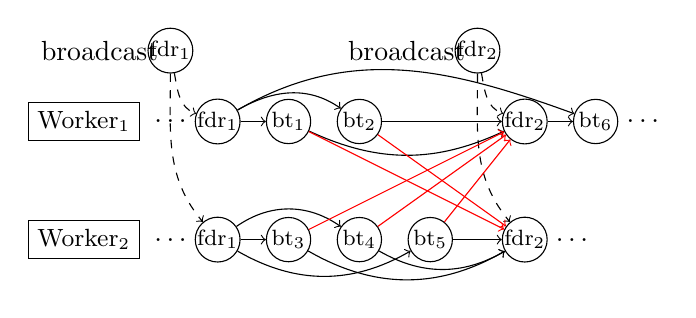
\begin{tikzpicture}[node distance=0.9cm and 0.9cm, on grid]
        %% Top Events
        \node[W] (w1) {$\textrm{Worker}_1$};
        \node[right=1.1 of w1] {$\ldots$};
        \node[B,right=1.7 of w1] (fdr1) {$\textrm{fdr}_1$};
        \node[B,right = of fdr1] (bt1) {$\textrm{bt}_1$};
        \node[B,right = of bt1] (bt2) {$\textrm{bt}_2$};
        \node[B,right=2.1 of bt2] (fdr2) {$\textrm{fdr}_2$};
        \node[B,right = of fdr2] (bt6) {$\textrm{bt}_6$};
        \node[right=0.6 of bt6] {$\ldots$};
        %% Bottom Events
        \node[W,below=1.5 of w1] (w2) {$\textrm{Worker}_2$};
        \node[right=1.1 of w2] {$\ldots$};
        \node[B,right=1.7 of w2] (fdr1') {$\textrm{fdr}_1$};
        \node[B,right = of fdr1'] (bt3) {$\textrm{bt}_3$};
        \node[B,right = of bt3] (bt4) {$\textrm{bt}_4$};
        \node[B,right = of bt4] (bt5) {$\textrm{bt}_5$};
        \node[B,right=1.2 of bt5] (fdr2') {$\textrm{fdr}_2$};
        \node[right=0.6 of fdr2'] {$\ldots$};
        %% Broadcasted events
        \node[B,above left=0.9 and 0.6 of fdr1] (fdr1root) {$\textrm{fdr}_1$};
        \node[left= of fdr1root] (broadcastfdr1) {$\textrm{broadcast}$};
        \draw[dashed,->] (fdr1root) to [out=280,in=160] (fdr1);
        \draw[dashed,->] (fdr1root) to [out=270,in=130] (fdr1');
        \node[B,above left=0.9 and 0.6 of fdr2] (fdr2root) {$\textrm{fdr}_2$};
        \node[left= of fdr2root] (broadcastfdr2) {$\textrm{broadcast}$};
        \draw[dashed,->] (fdr2root) to [out=280,in=160] (fdr2);
        \draw[dashed,->] (fdr2root) to [out=270,in=130] (fdr2');
        %% Top Edges
        \draw[E] (fdr1) -- (bt1);
        \draw[E] (fdr1) to [out=30,in=145] (bt2);
        \draw[E] (fdr1) to [out=30,in=160] (bt6);
        \draw[E] (bt2) -- (fdr2);
        \draw[E] (bt1) to [out=335,in=205] (fdr2);
        \draw[E] (fdr2) -- (bt6);
        %% Bottom Edges
        \draw[E] (fdr1') -- (bt3);
        \draw[E] (fdr1') to [out=35,in=145] (bt4);
        \draw[E] (fdr1') to [out=330,in=210] (bt5);
        \draw[E] (bt3) to [out=330,in=210] (fdr2');
        \draw[E] (bt4) to [out=330,in=210] (fdr2');
        \draw[E] (bt5) -- (fdr2');
        %% Cross-Dependency Edges
        \draw[red,->] (bt1) -- (fdr2');
        \draw[red,->] (bt2) -- (fdr2');
        \draw[red,->] (bt3) -- (fdr2);
        \draw[red,->] (bt4) -- (fdr2);
        \draw[red,->] (bt5) -- (fdr2);
        \end{tikzpicture}
        }
        % \centering
        % \includegraphics[width=\columnwidth]{cross-instance-dependencies.jpg}
        \caption{ML extension of fraud detection.}
        \label{fig:cross-instance-dependencies-vis}
	\end{subfigure}

% 	\begin{subfigure}[t]{0.8\columnwidth}
%         \centering
%         \includegraphics[width=\columnwidth]{cross-instance-dependencies.jpg}
%         \caption{ML extension of fraud detection.}
%         \label{fig:cross-instance-dependencies-vis}
% 	\end{subfigure}
    \caption{Illustration of an execution of two fraud detection
      examples and the event dependencies. Time progresses from left to right,
            different rows represent different parallel workers,
                  circles represent processing of
      events, dashed edges represent broadcasting an event,
            black edges represent dependencies, and red edges
      represent dependencies across parallel instances.
    %   \kk{Add an explanation of space-time in this diagram. That time moves from left to right etc.}
      }
    \label{fig:dependencies-vis}
\end{figure}



\paragraph{Fraud detection with a machine learning (ML) extension}
Consider a simple extension of the above application that is inspired
by today's ML workflows. In addition to user-input fraud detection
rules, the extended application also trains a model in an unsupervised
way using previously seen transactions. To achieve that the application keeps a sketch of previously seen bank transaction events. When a new fraud detection rule arrives, it aggregates the sketches and uses them to retrain the global fraud detection model.
As shown in
\Cref{fig:cross-instance-dependencies-vis},
this introduces dependencies across shards as the model retraining on rule events depends on all the previous bank transactions (even after broadcasting the rules), requiring communication between shards.

Unfortunately, standard ways of achieving data parallelism do not
support computations with such cyclic dependencies, leaving the user with two
unsatisfying solutions. They can either accept this
shortcoming and execute their computations with restricted parallelism---introducing
a throughput bottleneck in their application, or they can manually
implement the required synchronization using low level external
synchronization mechanisms (e.g. a key-value store with strong
consistency guarantees). This is error prone and, more importantly,
violates the implicit assumptions about the usage of
streaming APIs possibly leading to bugs and
erroneous behaviors.

\subsection{System Architecture}
\label{ssec:solution-architecture}

Our solution can achieve data parallelism for the extended fraud
detection application through the architecture
summarized in \Cref{fig:system-architecture-overview}.
The two primary abstractions (shown in blue) encode the required complex synchronization requirements at different levels of abstractions:
the DGS specification describes the computation and input dependencies
in a platform-independent manner,
and synchronization plans express the synchronization
between processes at the implementation level,
as communications between a hierarchically structured tree of processes.

The DGS specification is split in three parts.
First, the user
needs to provide a sequential implementation of the program, where the
input is assumed to arrive in order and one event at a time. The
sequential implementation consists of a stateful update function that
can output events and update its state every time an input event is
processed. For the fraud detection example, the update function would
process bank transactions by checking if they are fraudulent and by
constructing a sketch of the previously seen transactions, and fraud
detection rules by using the sketch of previously seen transactions
and the new rule to update the statistical fraud model. Second, the
user provides a dependence relation that indicates the input events
for which the processing order must be preserved, inducing a partial
order on input events. For the current example, the user would simply
indicate that fraud detection rule events depend on all other
events. The final part of a specification consists of primitives that
describe how to \emph{fork} the state into two independent copies to
allow for parallel processing and how to \emph{join} two states when
synchronization is required. These primitives abstractly represent
splitting the computation into independent computations and merging
the results, and are not tied to a specific implementation.

Given a DGS specification,
the mapping to the synchronization plan in our architecture
is given by a pluggable optimization component, which picks
a synchronization plan based on information about the target execution
environment, e.g. the number of processing workers and the location of
the input streams. All of the induced plans are shown to be correct with respect to the sequential specification, so the optimizer is free to pick any of them without endangering correctness. As a starting point, we have developed a simple
optimizer that tries to minimize the number of messages exchanged
between different workers using information about the execution
environment and the input streams.
As a final step, the synchronization plan abstraction
is deployed by the runtime system,
which among other implementation details enforces the ordering of input events based on input dependencies,
and is implemented in our DGSStream prototype.

\begin{figure}
  \centering
  \scalebox{.8}{
    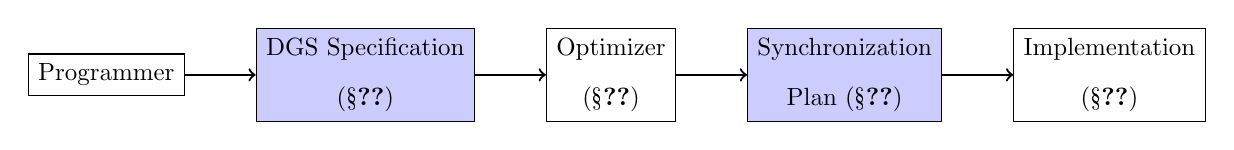
\begin{tikzpicture}[scale=0.9, transform shape, auto, node distance=1cm]
      \node[Block] (user) {Programmer};
      \node[Block,Data,Input,right=of user] (spec) {DGS Specification  \\ (\S\ref{sec:prog-model})};
      \node[Block,right=of spec] (opt) {Optimizer \\ (\S\ref{ssec:optimization-problem})};
    %   \node[Block,Data,Input,right=of opt] (top) {Target \\ Topology (\S\ref{sec:dist-impl})};
      \node[Block,Data,right=of opt] (cfg) {Synchronization \\ Plan (\S\ref{ssec:distributed-configurations})};
      \node[Block,right=of cfg] (impl) {Implementation \\ (\S\ref{ssec:runtime})};
      % \node[Block,right=3cm of cfg] (cd) {Code Distributor \\ (\S\ref{ssec:runtime})};
      % \node[Block,Output,below=1.5cm of cd] (impl) {Implementation};

      \draw[Block Edge] (user) -- (spec);
      \draw[Block Edge] (spec) -- (opt);
    %   \draw[Block Edge] (top) -- (opt);
    %   \draw[Block Edge] (top) -- (impl);
      \draw[Block Edge] (opt) -- (cfg);
      \draw[Block Edge] (cfg) -- (impl);
    \end{tikzpicture}
  }
  \caption{Architecture of the end-to-end DGS framework.
  }
\label{fig:system-architecture-overview}
\end{figure}

\subsection{Dependency-Guided Synchronization (DGS)}
\label{sec:prog-model}

A DGS specification consists of three components: a
\emph{sequential specification}, a \emph{dependence relation} on input
events to enforce synchronization, and \emph{fork} and \emph{join}
parallelization primitives.
At the end of the section we define specification \emph{consistency}, which are requirements on the \emph{fork} and \emph{join} functions to ensure that any parallelized implementation generated from the specification is equivalent to the sequential one.
As specifications are given programmatically,
we also refer to DGS as a \emph{programming model} and
to specifications as \emph{programs}.

\subsubsection{Walkthrough}

For a simple but illustrative example, suppose that we want to
implement a stream processing application that simulates a map from
keys to counters, in which there are two types of input events: \emph{increment}
events, denoted $\tg{i}(k)$, and \emph{read-reset} events, denoted
$\tg{r}(k)$, where each event has an associated key $k$.  On each
increment event, the counter associated with that key should be
increased by one, and on each read-reset event, the current value of
the counter should be produced as output, and then the counter should be reset to
zero.
The ``type'' of an input event is called its \emph{tag}, and in this example there are
two tags.
An input event may also carry a \emph{payload} of data that is not
used for parallelization. In this example all events have an empty payload.

\paragraph{Sequential specification.}
\label{p:seq-impl}
In our programming model, the user first provides a sequential
implementation of the desired computation.
A pseudocode version of the sequential specification for the
example above is shown in \Cref{fig:key-value-store} (left). It consists of
(i) the state type \fl{State}, i.e. the map from keys to
counters, (ii) the initial value of the state \fl{init},
i.e. $0$ for all keys, and (iii) a function \fl{update},
which contains the logic for processing input events.
Conceptually, the sequential specification describes how to process
the data assuming it was all combined into a single sequential stream (e.g.,
sorted by system timestamp).  For example, if the input stream
consists of the events $\tg{i}(1), \tg{i}(2), \tg{r}(1), \tg{i}(2),
\tg{r}(1)$, then the output would be $1$ followed by $0$, produced by
the two $\tg{r}(1)$ (read-reset) events.

\begin{figure}[t]
\centering \footnotesize{}
\begin{minipage}{0.38\textwidth}
\begin{FluminaCode}
// Types
Key = Integer
Tag = i(Key) | r(Key)
Payload = ()
Event = (Tag, Payload)
State = Map(Key, Integer)




// Sequential Implementation
init: () -> State
init() =
    return emptyMap()
update: (State, Event) -> State
update(s, (i(k), ())) =
    s[k] = s[k] + 1;
    return s
update(s, (r(k), ())) =
    output s[k];
    s[k] = 0;
    return s
\end{FluminaCode}
\end{minipage}
\begin{minipage}{0.6\textwidth}
\begin{FluminaCode}
// Dependence Relation
dependencies: (Tag, Tag) -> Bool
dependencies(r(k1), r(k2)) = k1 == k2
dependencies(r(k1), i(k2)) = k1 == k2
dependencies(i(k1), r(k2)) = k1 == k2
dependencies(i(k1), i(k2)) = false

// Fork and Join
fork: (State, Tag -> Bool, Tag -> Bool) -> (State, State)
fork(s, pred1, pred2) =
    s1 = init(); s2 = init() // two forked states
    for k in keys(s):
        if pred1(r(k)):
            s1[k] = s[k]
        else: // pred2(r(k)) OR r(k) in neither
            s2[k] = s[k]
    return (s1, s2)
join: (State, State) -> State
join(s1, s2) =
    for k in keys(s2):
        s1[k] = s1[k] + s2[k]
    return s1
\end{FluminaCode}
\end{minipage}


\caption{
  Specification in DGS of a map from keys to counters, which
  can process increment operations $\tg{i}(k)$ and read-reset
  operations $\tg{r}(k)$ for each key $k$.
  Erlang syntax has been
  edited for readability.
  We use \fl{s[k]} as shorthand for getting key $k$ from the map
  \emph{or} the default value $0$ if it is not present.
}
\label{fig:key-value-store}
\end{figure}

\begin{figure}
    \centering
    \scriptsize{}
    \begin{tabular}{cc}
        \TwoTagDepGraph{\tg{r}(1)}{\tg{i}(1)}{\draw (1) edge[Tag Loop] (1); \draw (1) edge[Tag Edge] (2);}
      & \TwoTagDepGraph{\tg{r}(2)}{\tg{i}(2)}{\draw (1) edge[Tag Loop] (1); \draw (1) edge[Tag Edge] (2);} \\
        % \TwoTagDepGraph{\tg{r}(3)}{\tg{i}(3)}{\draw (1) edge[Tag Loop] (1); \draw (1) edge[Tag Edge] (2);} \\
        \multicolumn{2}{c}{$\cdots$}
    \end{tabular}
    \captionof{figure}{The \fl{dependencies} relation from \Cref{fig:key-value-store}
    visualized as a graph, with 2 keys shown.
    Edges enforce synchronization requirements, while non-edges expose parallelism.}
    \label{fig:key-value-store-dependencies}
\end{figure}

\paragraph{Dependence relation.}
%
To parallelize a sequential computation, the user needs to provide a
dependence relation which encodes which events are independent, and
thus can be processed in parallel, and which events are dependent, and
therefore require synchronization.  The dependence relation abstractly
captures all the dependency patterns that appear in an application,
inducing a partial order on input events. In this example, there are
two forms of independence we want to expose. To begin with,
\emph{parallelization by key} is possible: the counter map could be
partitioned so that events corresponding to different sets of keys are processed
independently. Moreover, \emph{parallelizing increments} on the
counter of the same key is also possible. In particular, different
sets of increments for the same key can be processed independently; we
only need to aggregate the independent counts when a read-reset
operation arrives. On the other hand, read-reset events
are synchronizing for a particular key;
their output is affected by the processing of increments
as well as other read-reset events of that key.

% \begin{figure}
% \centering \scriptsize{}
% \begin{tabular}{cccc}
%   \TwoTagDepGraph{\tg{r}(1)}{\tg{i}(1)}{\draw (1) edge[Tag Loop] (1); \draw (1) edge[Tag Edge] (2);}
% & \TwoTagDepGraph{\tg{r}(2)}{\tg{i}(2)}{\draw (1) edge[Tag Loop] (1); \draw (1) edge[Tag Edge] (2);}
% & \TwoTagDepGraph{\tg{r}(3)}{\tg{i}(3)}{\draw (1) edge[Tag Loop] (1); \draw (1) edge[Tag Edge] (2);}
% & $\cdots$
% \end{tabular}
% \caption{The \fl{dependencies} relation from \Cref{fig:key-value-store}
% visualized as a graph, with 3 keys shown.
% Edges enforce synchronization requirements, while non-edges expose parallelism.}
% \label{fig:key-value-store-dependencies}
% \end{figure}

We capture this combination of parallelization and synchronization
requirements by defining the dependence relation
\fl{dependencies} in \Cref{fig:key-value-store}, which is
also visualized in \Cref{fig:key-value-store-dependencies}.
In the specification, the set of tags may be \emph{symbolic}
(infinite): here \fl{Tag} is parameterized by an integer \fl{Key}.
To allow for this, the dependence relation
is formally a \emph{predicate} on pairs of tags,
and is given programmatically as a function from pairs
of \fl{Tag} to \fl{Bool}.
For example, \fl{dependencies(r(k1), r(k2))} (one of four cases)
is given symbolically as equality comparison of keys, \fl{k1 == k2}.
The dependence relation should also be \emph{symmetric},
i.e. \fl{e1} is in \fl{dependencies(e2)} if and
only if \fl{e2} is in \fl{dependencies(e1)}.

\paragraph{Parallelization primitives: \emph{fork} and \emph{join}.}
\label{p:fork-join}
%
While the dependence relation indicates the possibility of
parallelization, it does not provide a mechanism for parallelizing
state.  The parallelization is specified using a pair of functions to \fl{fork}
one state into two, and to \fl{join} two states into one.
The
fork function additionally takes as input two predicates of tags,
such that the two predicates are \emph{independent} (but not necessarily disjoint):
every tag satisfying \fl{pred1} is independent of every tag satisfying \fl{pred2}.
The
contract is that after the state is forked into two independent
states, each state will then \emph{only be updated using events from
the given set of tags.}
A fork-join specification for our example
is shown in~\cref{fig:key-value-store}.
The \fl{join} function simply adds up the counts for each key to form the combined
state. The \fl{fork} function has to decide, for each key, which forked state
to send the count to.
Since read-reset operations \fl{r(k)} are synchronizing and require knowing the total count,
it does this by checking
which forked state is responsible for processing read-reset
operations, if any.

It is necessary that the \fl{fork} function
have the predicates \fl{pred1} and \fl{pred2} as input,
as otherwise we would not know how to partition the state \fl{s}
in case of \emph{parallelization by key}.
For example, if \fl{pred1} contains all events of key $1$
and \fl{pred2} contains all events of key $2$,
then we need to propagate the count \fl{s[1]} to the first forked state
and the count \fl{s[2]} to the second forked state.
However, it is also possible that \fl{pred1} and \fl{pred2}
are \emph{not} disjoint,
which is necessary to accommodate \emph{parallelization by increment}.
For example, \fl{pred1} and \fl{pred2} may both contain \fl{i(3)}
events.
This is the reason that we include both \fl{pred1} and \fl{pred2},
even though only \fl{pred1} is used in our example.
Fortunately in this case, the independence requirement
guarantees that neither forked state will be responsible for
\fl{r(3)} events (as \fl{r(3)} is dependent on \fl{i(3)});
in particular, neither forked state will be required to produce output for key $3$.
Therefore, we can choose to propagate the count \fl{s[3]} to either state,
knowing that the two forked counts will later be added back together in \fl{join}.
% as long as we ensure the counts are added when the states are joined back together.
This illustrates that the fork function's input can indicate either
a partitioning of input events, or parallelization on events on the same tag
(or a combination of these across different keys).
% This information is encoded using a pair of predicates
% (and cannot be encoded using only one).


% For our specific example, the guarantee is that only one of two
% forked states will be assigned to process read-reset events for a key. If the
% input $\tg{r}(k)$ is in \fl{tags1}, then we know that
% updates of key $k$ will all be processed by the first state, and so we
% copy the value for this key to the first state. Conversely, if the
% input $\tg{r}(k)$ is in \fl{tags2}, we copy the value for
% this key to the second state.  The third case is that the input
% $\tg{r}(k)$ is in neither \fl{tags1} nor
% \fl{tags2}; then we can copy the value to \emph{either} the
% first or the second state. In this case, both states may receive
% increment events. This is acceptable because before any read-reset
% operation can be processed, the \fl{join} function will be
% called, which adds the two totals back together again.

\begin{figure}
\centering \scriptsize{}
% \scalebox{0.8}{
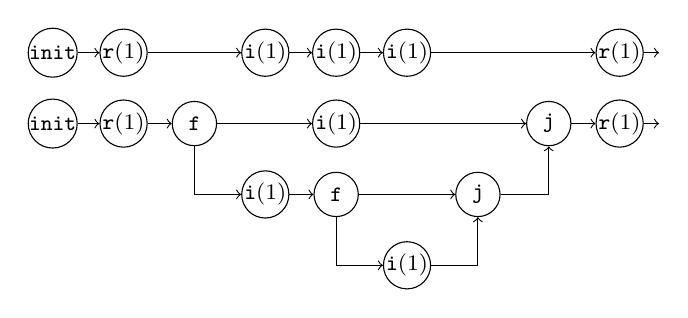
\begin{tikzpicture}[node distance=0.9cm and 0.9cm, on grid]
%% Bottom Nodes
\node[B] (0) {$\istate$};
\node[B,right = of 0] (1) {${\tg{r}(1)}$};
\node[B,right = of 1] (2) {$\fk$};
\node[B,below right = of 2] (2b) {${\tg{i}(1)}$};
\node[B,right = of 2b] (3) {$\fk$};
\node[B,above = of 3] (2a) {${\tg{i}(1)}$};
\node[B,below right = of 3] (3b) {${\tg{i}(1)}$};
\node[B,above right = of 3b] (4) {$\jn$};
\node[B,above right = of 4] (5) {$\jn$};
\node[B,right = of 5] (6) {${\tg{r}(1)}$};
\coordinate[right=0.5cm of 6] (7);
%% Top Nodes
\node[B,above = of 0] (t0) {$\istate$};
\node[B,right = of t0] (t1) {${\tg{r}(1)}$};
\node[B,above right = of 2] (t2) {${\tg{i}(1)}$};
\node[B,right = of t2] (t3) {${\tg{i}(1)}$};
\node[B,right = of t3] (t4) {${\tg{i}(1)}$};
\node[B,above = of 6] (t5) {${\tg{r}(1)}$};
\coordinate[right=0.5cm of t5] (t6);
%% Bottom Edges
\draw[E] (0) -- (1);
\draw[E] (1) -- (2);
\draw[E] (2) -- (2a);
\draw[E] (2) |- (2b);
\draw[E] (2b) -- (3);
\draw[E] (3) -- (4);
\draw[E] (3) |- (3b);
\draw[E] (3b) -| (4);
\draw[E] (4) -| (5);
\draw[E] (2a) -- (5);
\draw[E] (5) -- (6);
\draw[E] (6) -- (7);
%% Top Edges
\draw[E] (t0) -- (t1);
\draw[E] (t1) -- (t2);
\draw[E] (t2) -- (t3);
\draw[E] (t3) -- (t4);
\draw[E] (t4) -- (t5);
\draw[E] (t5) -- (t6);
\end{tikzpicture}
% }
\caption{Example of a sequential and parallel execution of the program in \cref{fig:key-value-store} on the input stream $\tg{r}(1), \tg{i}(1), \tg{i}(1), \tg{i}(1), \tg{r}(1)$. Here $k = 1$ is a key, and
$\fk$ and $\jn$ denote fork and join functions.
\emph{\textbf{Top:} Sequential execution: each item of the input stream is processed as an update to a global state. \textbf{Bottom:} One possible parallel execution: in between some updates, the state is forked or joined, and $\tg{i}$ events are processed as independent updates to one of the forked states.}}
\label{fig:example-wire-diagram}
\end{figure}

\subsubsection{Formal Definition}

A DGS specification can be more general than we have discussed so far,
because we allow for multiple \emph{state types}, instead of just
one. The initial state must be of a certain type, but forks and joins
can convert from one state type to another: for example, forking a
pair into its two components.
Additionally,
each state type can come with a \emph{predicate} which restricts
the allowed tags processed by a state of that type.
The complete programming model is summarized in the following
definition.

\begin{definition}[DGS Specification]
\label{def:prog-model}
Let \fl{Pred(T)} be a given type of \emph{predicates}
on a type \fl{T},
where predicates denote functions \fl{T -> Bool}.
A specification consists of the following components:
\begin{enumerate}[(1)]
\item A type of input events \fl{Event = (Tag, Payload)},
where \fl{Tag} is a type of tags.
\item The dependence relation \fl{dependencies: Pred(Tag, Tag)},
which is symmetric: \fl{dependencies(tag1, tag2)}
iff \fl{dependencies(tag2, tag1)}.
\item A type for output events \fl{Out}.
\item Finitely many state types \fl{State_0}, \fl{State_1}, etc.
\item For each state type \fl{State_i},
a predicate \fl{pred_i: Pred(Tag)} --- this specifies which input values this type of state can process --- where \fl{pred_0} $=$ \fl{true}.
\item A sequential implementation, consisting of a single initial state \fl{init: State_0} and for each state type \fl{State_i},
a function \fl{update_i: (State_i, Event) -> State_i}.
The update also produces zero or more outputs, given formally by a function
\fl{out_i: (State_i, Event) -> List(Out)}.
\item Any number of parallelization primitives, where each is either a \emph{fork} or a \emph{join}. A fork function has type
\fl{(State_i, Pred(Tag), Pred(Tag)) -> (State_j, State_k)},
and a join function has type
\fl{(State_j, State_k) -> State_i}, for some $i, j, k$.
\end{enumerate}
\end{definition}

The semantics of a specification
can be visualized using wire
diagrams, as in \Cref{fig:example-wire-diagram}. Computation proceeds from left to right. Each wire is associated with
(i) a state (of type \fl{State_i} for some $i$) and
(ii) a predicate on tags (of type \fl{Pred(Tag)})
which restricts the input events that this wire can process.
Input events are processed as
updates to the state, which means they take one input wire and produce
one output wire, while forks take one input wire and produce two, and
joins take two input wires and produce one. Notice that the same updates are present in both sequential and parallel executions. It is guaranteed in the
parallel execution that \emph{fork and join come in pairs}, like
matched parentheses. Each predicate on tags that is given as input to the \fl{fork} function indicates the set of input events that can be processed along one of the outgoing wires.
Additionally, we require that updates on parallel wires must be
on independent tags.
In the example,
the wire is forked into two parts and then forked again, and all three
resulting wires process $\tg{i}(1)$ events. Note that $\tg{r}(1)$
events cannot be processed at that time because they are dependent on
$\tg{i}(1)$ events.
More specifically, we require that
the predicate at each wire of type \fl{State_i}
implies \fl{pred_i}, and that
after each \fl{fork} call,
the predicates at each resulting wire denote independent sets of tags.
This semantics is formalized in the following definition.

\begin{definition}[DGS Semantics]
\label{def:prog-model-semantics}
A \emph{wire} is a triple
\wire{\fl{State_i}}{\fl{pred}}{\fl{s}},
where
\fl{State_i} is a state type,
\fl{s: State_i},
and \fl{pred: Pred(Tag)}
is a predicate of allowed tags,
such that \fl{pred} implies \fl{pred_i}.
We give the semantics of a specification through an
inductively defined relation, which we denote
\semantics{\fl{State}}{\fl{pred}}{\fl{s}}{\fl{u}}{\fl{s'}}{\fl{v}},
where
\wire{\fl{State}}{\fl{pred}}{\fl{s}} and \wire{\fl{State}}{\fl{pred}}{\fl{s'}}
are the starting and ending wires
(with the same state type and predicate),
\fl{u: List(Event)} is an input stream,
and \fl{v: List(Out)} is an output stream.
Let \fl{l1 + l2} be list concatenation, and
define \fl{inter(l, l1, l2)} if \fl{l} is some interleaving of \fl{l1} and \fl{l2}.
For \fl{e1}, \fl{e2: Event},
let \fl{indep(e1, e2)} denote that
\fl{e1} and \fl{e2} are not dependent, i.e.
\fl{not(dependencies(}\fst{\fl{e1}}\fl{,}\fst{\fl{e2}}\fl{))}.
There are two base cases and two inductive cases.
\begin{itemize}
\item (Emp)
For any \fl{State}, \fl{pred}, and \fl{s},
\semantics{\fl{State}}{\fl{pred}}{\fl{s}}{\fl{[]}}{\fl{s}}{\fl{[]}}.
\item (Upd)
For any \fl{State}, \fl{pred}, \fl{s}, and any \fl{e: Event},
if the tag of \fl{e} satisfies \fl{pred}, i.e.
\fl{pred(}\fst{\fl{e}}\fl{)}, then
\semantics{\fl{State}}{\fl{pred}}{\fl{s}}{\fl{[e]}}{\fl{update(s, e)}}{\fl{out(s, e)}}.
\item (Seq)
For any \fl{State}, \fl{pred}, \fl{s}, \fl{s'}, \fl{s''},
\fl{u}, \fl{v}, \fl{u'}, and \fl{v'}, if
\semantics{\fl{State}}{\fl{pred}}{\fl{s}}{\fl{u}}{\fl{s'}}{\fl{v}}
and
\semantics{\fl{State}}{\fl{pred}}{\fl{s'}}{\fl{u'}}{\fl{s''}}{\fl{v'}},
then
\semantics{\fl{State}}{\fl{pred}}{\fl{s}}{\fl{u + u'}}{\fl{s''}}{\fl{v + v'}}.
\item (Par)
Lastly, for any
\fl{State}, \fl{State1}, \fl{State2},
\fl{pred}, \fl{pred1}, \fl{pred2},
\fl{s},
\fl{s1'}, \fl{s2'},
\fl{u}, \fl{u1}, \fl{u2}, \fl{v}, \fl{v1}, \fl{v2},
\fl{fork}, and \fl{join},
suppose that
(the conjunction) \fl{pred1(e1)} and \fl{pred2(e2)} implies
\fl{indep(e1, e2)},
\fl{pred1} implies \fl{pred}, and
\fl{pred2} implies \fl{pred}.
Let
\fl{fork(s, pred1, pred2) = (s1, s2)}
and
\fl{join(s1', s2') = s'},
and suppose that
\fl{inter(u, u1, u2)}
and
\fl{inter(v, v1, v2)}.
If
\semantics{\fl{State1}}{\fl{pred1}}{\fl{s1}}{\fl{u1}}{\fl{s1'}}{\fl{v1}}
and
\semantics{\fl{State2}}{\fl{pred2}}{\fl{s2}}{\fl{u2}}{\fl{s2'}}{\fl{v2}}
then
\semantics{\fl{State}}{\fl{pred}}{\fl{s}}{\fl{u}}{\fl{s'}}{\fl{v}}.
\end{itemize}
The \emph{semantics} $\sem{S}$ of the specification $S$
is the set of pairs $(\fl{u}, \fl{v})$
of an input stream \fl{u} and an output stream \fl{v} such that
\semantics{\fl{State_0}}{\fl{true}}{\fl{init}}{\fl{u}}{\fl{s'}}{\fl{v}}
for some final state \fl{s'}.
\end{definition}

\subsubsection{Consistency of Specifications}
\label{ssec:prog-model-correctness}

Any parallel execution
is guaranteed to preserve the sequential semantics, i.e. processing
all input events \emph{in order} using the \fl{update} function,
as long as the following \emph{consistency conditions} are
satisfied.
The sufficiency of these conditions is shown in
\Cref{thm:consistency-implies-determinism}, which states
that \emph{consistency implies determinism up to output reordering}.
This is a key step in the end-to-end proof of correctness in \Cref{ssec:proof-of-correctness}.
Consistency can be thought of as analogous to the commutativity and
associativity requirements for a MapReduce program to have
deterministic output~\cite{dean2008mapreduce}: just as with MapReduce
programs, the implementation does \emph{not} assume the conditions are
satisfied, but if not the semantics will be dependent on how the
computation is parallelized.

Let us briefly illustrate the consistency conditions for our running example
(\Cref{fig:key-value-store}).
% consider (C1), which states that joins commute with updates.
If \fl{e} is an increment event,
then condition (C1) captures the fact that counting can be done in parallel:
it reduces to $\fl{(s1[k] + s2[k]) + 1} = \fl{(s1[k] + 1) + s2[k]}$.
% For a read-reset event, this holds due to an invariant on the state
% s2[k] that it must be 0 for that key because the key for s1[0] is 0.
Condition (C2) captures the fact that we preserve total count
across states when forking: it reduces to $\fl{s[k] + 0} = \fl{s[k]}$.
Condition (C3) would not be valid for \emph{general} events
\fl{e1}, \fl{e2}, because a read-reset event does not commute with an increment
of the same key ($\fl{s[k] + 1} \ne \fl{s[k]}$),
hence the restriction that \fl{indep(e1, e2)}.
Finally, one might think that a variant of (C1) should hold for
\fl{fork} in addition to \fl{join},
but this turns out not to be the case:
for example, starting from $\fl{s[k] = 100}$,
an increment followed by a fork might yield the pair of counts
$(101, 0)$, while a fork followed by an increment might yield
$(100, 1)$.
It turns out however that commutativity only with joins, and not with
forks, is enough to imply \Cref{thm:consistency-implies-determinism}.

\begin{definition}[Consistency]
\label{def:prog-model-consistency}
A specification is \emph{consistent} if the following
equations always hold:
\begin{align*}
\fl{join(update(s1, e), s2)}
    &\;= \fl{update(join(s1, s2), e)} \tag{C1} \\
\fl{join(fork(s, pred1, pred2))}
    &\;= \fl{s} \tag{C2} \\
\fl{update(update(s, e1), e2))}
    &\;= \fl{update(update(s, e2), e1))}. \tag{C3}
\end{align*}
Equation (C1)
is over all
join functions \fl{join: (State_j, State_k) -> State_i},
events \fl{e: Event} such that \fl{pred_i(e)} and \fl{pred_j(e)},
and states \fl{s1: State_j}, \fl{s2: State_k},
where \fl{update} denotes the update function on the appropriate type.
Additionally the corresponding output on both sides must be the same:
$\fl{out(s1, e)} = \fl{out(join(s1, s2))}$.
Equation (C2)
is over all
fork functions \fl{fork: (State_i, Pred(Tag),} \fl{Pred(Tag)) -> (State_j, State_k)}
join functions \fl{join: (State_j, State_k) -> State_i},
states \fl{s: State_i}, and predicates \fl{pred1} and \fl{pred2}.
Equation (C3)
is over all state types \fl{State_i},
states \fl{s: State_i},
and \emph{independent} events
\fl{indep(e1, e2)}
such that \fl{pred_i(e1)} and \fl{pred_i(e2)}.
As with (C1), we also require that the outputs
agree:
$\fl{out(s, e1) + out(update(s, e1), e2) = out(update(s, e2), e1) + out(s, e2)}$.
\end{definition}


%% Form of definition using enumerate
% \begin{definition}[Consistency]
% \label{def:prog-model-consistency}
% A specification is \emph{consistent} if the following
% three conditions hold.
% \begin{enumerate}[(1)]
% \item
% For all
% join functions \fl{join: (State_j, State_k) -> State_i},
% events \fl{e: Event} such that \fl{pred_i(e)} and \fl{pred_j(e)},
% states \fl{s1: State_j} and \fl{s2: State_k},
% where \fl{update} denotes the update function on the appropriate type:
% \[
% \fl{join(update(s1, e), s2)} = \fl{update(join(s1, s2), e)}, \tag{1}
% \]
% and the corresponding output on both sides is the same:
% $\fl{out(s1, e)} = \fl{out(join(s1, s2))}$.
% \item
% For all
% fork functions \fl{fork: (State_i, Pred(Tag), Pred(Tag)) -> (State_j, State_k)}
% join functions \fl{join: (State_j, State_k) -> State_i},
% states \fl{s: State_i}, and predicates \fl{pred1} and \fl{pred2},
% \[
% \fl{join(fork(s, pred1, pred2))} = \fl{s}. \tag{2}
% \]
% \item
% For all state types \fl{State_i},
% states \fl{s: State_i},
% and events \fl{e1}, \fl{e2: Event}
% such that \fl{pred_i(e1)} and \fl{pred_i(e2)},
% \emph{if} \fl{indep(e1, e2)} then
% \[
% \fl{update(update(s, e1), e2))} = \fl{update(update(s, e2), e1))}, \tag{3}
% \]
% and the corresponding output on both sides
% is the same:
% $\fl{out(s, e1)} + \fl{out(update(s, e1), e2)}
% = \fl{out(update(s, e2), e1)} + \fl{out(s, e2)}$.
% \end{enumerate}
% \end{definition}

%% Definition using single align* equation for all 5 conditions
% for all functions \fl{update}, \fl{out}, \fl{join}, and \fl{fork}
% in the specification:
% \begin{align*}
% \fl{join(update(s1, e), s2)}
%     =\;& \fl{update(join(s1, s2), e)}
%     \tag{1a} \\
% \fl{out(s1, e)}
%     =\;& \fl{out(join(s1, s2))}
%     \tag{1b} \\
% \fl{join(fork(s, pred1, pred2))}
%     =\;& \fl{s} \tag{2} \\
% \fl{update(update(s, e1), e2))}
%     =\;& \fl{update(update(s, e2), e1))}
%     \tag{3a} \\
% \fl{out(s, e1)} + \fl{out(update(s, e1), e2)}
%     =\;& \fl{out(update(s, e2), e1)} + \fl{out(s, e2)}
%     \tag{3b}
% \end{align*}

\begin{theorem}
\label{thm:consistency-implies-determinism}
If $S$ is consistent, then $S$ is deterministic up to output reordering:
that is,
for all $(\fl{u}, \fl{v}) \in \sem{S}$,
\fl{set(v) = set(spec(u))}.
\end{theorem}
\begin{proof}
We show by induction on the semantics in \Cref{def:prog-model-semantics}
that every wire diagram is equivalent (up to output reordering) to the sequential sequence
of updates.
The (Seq) inductive step is direct by associativity of function composition
on the left and right sequence of updates (no commutativity of updates is required).
For the (Par) inductive step, we replace the two parallel wires with sequential wires,
then apply (C1) repeatedly on the last output to move it outside of the parallel wires,
then finally apply (C2) to reduce the now trivial parallel wires to a single wire.
% Caleb: I think that consistency condition C3 is actually unused, interestingly enough.
% I won't mention it in the proof sketch since I might have missed something.
\end{proof}

\subsection{Distributed Implementation}
\label{sec:dist-impl}

This section describes the distributed runtime for DGS.
In particular, we describe \emph{synchronization plans},
which represent streaming program implementations, and our
framework for generating them from the given DGS specification
in \cref{sec:prog-model}.
Generation of an implementation can be
conceptually split in two parts, the first ensuring correctness and
the second affecting performance. First a specification $S$ induces a set of
$S$-\emph{valid}, i.e. correct with respect to it, synchronization
plans. Choosing one of those plans is then an independent optimization
problem that does not affect correctness and can be delegated to a
separate optimization component (\cref{ssec:optimization-problem}).
Finally, the workers in synchronization plans
need to process some incoming events in order while some can be
processed out of order (depending on the dependence relation).  We
propose a selective reordering technique
(\cref{ssec:runtime}) that can be used in tandem with heartbeats to
address this ordering issue.
We tie everything together by providing an end-to-end proof that the
implementation is correct with respect to a consistent specification
$S$ (and importantly, independent of the synchronization plan chosen
as long as it is $S$-valid) in \cref{ssec:proof-of-correctness}.
Before describing the separate framework components, we first
articulate the necessary underlying assumptions about input streams in
\cref{ssec:distributed-assumptions}.

\subsubsection{Preliminaries}
% \subsubsection{Streaming Assumptions}
\label{ssec:distributed-assumptions}

In our model the input is partitioned in some number of input streams that could be distributed, i.e. produced at different locations.
We assume that the implementation has access to \emph{some} ordering
relation $\mathcal{O}$ on pairs of input events (also denoted
$<_{\mathcal{O}}$), and the order of events is increasing along each
input stream. This is necessary for cases where the
\emph{user-written} specification requires that events arriving in
different streams are dependent, since it allows the implementation to
have progress and process these dependent events in order.
Concretely, in our setting $\mathcal{O}$ is implemented using \emph{event timestamps}.
Note that these timestamps do not need to correspond to real time, if this is not required by the application.
In cases where real-time timestamps are required, this can be achieved with well-synchronized clocks, as has been done in other systems, e.g. Google Spanner~\cite{corbett2013spanner}.

%% % To clarify why this is not overly restrictive, suppose for example that the implementation has two streams arriving at different nodes, and some events $x_1$ and $x_2$ arrive on stream 1 and stream 2, respectively. There are two cases. First if $x_1$ and $x_2$ are independent (and the user has written a fork function), then the system could fork state to process them in parallel, so the order relation is ignored and not necessary. Second, if they are dependent, then this means that we need to synchronize and process $x_1$ and $x_2$ sequentially.
%% % In this synchronizing case, we process $x_1$ first if $x_1 <_{\mathcal{O}} x_2$ and $x_2$ first if $x_2 <_{\mathcal{O}} x_1$, irrespective of the time that $x_1$ and $x_2$ arrive in the system, which makes the execution deterministic.
%% % The increasing condition (2) is necessary to ensure progress: in the synchronizing case, note that we can't process $x_2$ until we know know no earlier events will occur. Because of increasing timestamps, this holds when we receive any event $x_1'$ on the first node such that $x_1' >_{\mathcal{O}} x_2$.
%% There are cases where ordering between distributed nodes is useful,
%% and in this case our assumption of an order relation is conservative.
%% For example, it is weaker than assuming synchronized clocks, as event
%% timestamps do not need to correspond to real time.
%% % , e.g. in the above example if $x_2 <_{\mathcal{O}} x_1$.
%% If the user does require near real-time timestamps, the assumption of well-synchronized clocks has been justified by other systems, e.g. Google Spanner~\cite{corbett2013spanner}.

Each event in each input stream is given by a triple $\langle \sigma, ts, v \rangle$,
containing an \emph{implementation tag}
$\sigma \in \fl{ITag}$, a timestamp $ts$, and its payload $v$.
Each implementation tag corresponds to one or more tags in the specification in \cref{sec:prog-model}, but is also augmented with an identifier of the input stream.
This ensures that each implementation tag is unique to a particular input stream, while a tag can appear in multiple streams (in all of the streams with a corresponding implementation tag).
To simplify the presentation in this section, we assume that the set of implementation tags is finite, and this is also currently required in our prototype implementation.
A dependence relation $\fl{dependencies}$ straightforwardly lifts from tags in the specification to predicates over tags and to implementation tags $D_I \subseteq \fl{ITag} \times \fl{ITag}$.
% \caleb{Is this good?
% I don't know how to say anything else without it sounding bad.
% I will make a note to revisit this for final version.
% I also wanted to just not update the rest of this section so decided not
% to try to make the synchronization plans work with predicates directly. }

\subsubsection{Synchronization Plans}
\label{ssec:distributed-configurations}

Synchronization plans are binary tree structures that encode (i)
parallelism: each node of the tree represents a sequential thread of
computation that processes input events; and (ii) synchronization:
parents have to synchronize with their children to process an event.
Synchronization plans are inspired by prior work on concurrency
models including fork-join concurrency~\cite{frigo1998implementation,lea2000java} and
CSP~\cite{hoare1978communicating}. An example synchronization plan for
the specification in \Cref{fig:key-value-store} is shown in
\Cref{fig:example-configuration}.  Each node has an id $w_i$, contains
the set of implementation tags that it is responsible for, a state
type (which is omitted here since there is only one state type
\texttt{State}), and a triple of update, fork, join functions.
% , and the physical node $N_i$ at which the worker is allocated.
Note that a node is responsible to process events from its set of
implementation tags, but can potentially handle all the implementation
tags of its children. The leaves of the tree can process events
independently without blocking, while parent nodes can only process an
input event if their children states are joined. Nodes without a
ancestor-descendant relationship do not directly communicate, but
instead learn about each other when their common ancestor
joins and forks back the state.

\newcommand{\wfield}[2]{{#1}.{\mathsf{#2}}}

\begin{definition}[Synchronization Plans]
  Given a specification $S$,
  a synchronization plan is a pair $(\overline{w}, \mathrm{par})$,
  which includes a set of workers $\overline{w} = \{ w_1, \ldots, w_N \}$,
  where $w_i \in W$,
  together with a parent relation $\mathrm{par} \subseteq W \times W$,
    the transitive closure of which is an ancestor relation denoted as
    $\mathrm{anc} \subseteq W \times W$.
  Workers have three components:
    (i) a state type $\wfield{w}{state}$ which references one of the state types of $S$,
    (ii) a set of implementation tags $\wfield{w}{itags}$ that the worker is responsible for,
    and (iii) an update $\wfield{w}{update}$ and possibly a fork-join pair $\wfield{w}{fork}$ and $\wfield{w}{join}$ if it has children.
\end{definition}

\begin{figure}
\scalebox{0.8}{
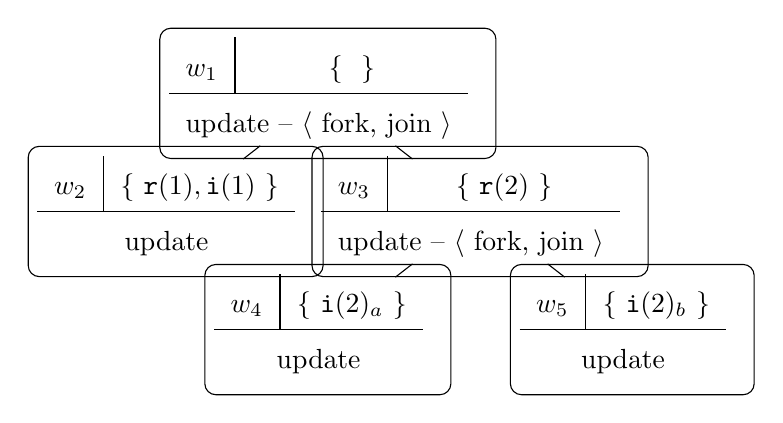
\begin{tikzpicture}[sibling distance=11em,
  every node/.style = {shape=rectangle,
    rounded corners,
    draw, align=center}]]
  \node { \TopConfigNode{$w_1$}{}{update -- $\langle$ fork, join $\rangle$} }
    child { \ConfigurationNode{$w_2$}{$\tg{r}(1), \tg{i}(1)$}{update} }
    child { \ConfigurationNode{$w_3$}{$\tg{r}(2)$}{update -- $\langle$ fork, join $\rangle$}
        child { \ConfigurationNode{$w_4$}{$\tg{i}(2)_a$}{update} }
        child { \ConfigurationNode{$w_5$}{$\tg{i}(2)_b$}{update} } };
%   \node (node0) [above=1mm of e0.north west, draw=none] { $E_0$ };
%   \node [draw=black!50, fit={(e0) (e23) (node0)}, rounded corners=0] (c0) {};
\end{tikzpicture}
}
\caption{Example synchronization plan derived from the
  specification in \Cref{fig:key-value-store} for two keys $k=2$ and
  five input streams $\tg{r}(1), \tg{i}(1), \tg{r}(2), \tg{i}(2)_a, \tg{i}(2)_b$.
  Implementation tags $\tg{i}(2)_a, \tg{i}(2)_b$ both correspond to the tag $\tg{i}(2)$ but are separate because they arrive in different input streams.
  Each node contains the set of implementation tags that it is responsible for,
  an update function, and a pair of fork-join
  functions if it has children.
  % \kk{Reviewer C: notation seems different from Figure 2, let's discuss why.}
  }
\label{fig:example-configuration}
\end{figure}

% \kk{Restructure this}
% Let \fl{ITag} be the set of implementation tags,
% where each specification tag corresponds to at
% least one implementation tag $\sigma \in \fl{ITag}$
% % TODO maybe add this
% % and each implementation tag corresponds to exactly one specification tag,
% and the dependence relation is
% extended to $D_I \subseteq \fl{ITag} \times \fl{ITag}$.
% Given the computation specification
% and any additional information needed by the optimizer,
% our framework produces a synchronization
% plan $(\overline{w}, \mathrm{par})$ which is a set of workers $\overline{w} = \{ w_1, \ldots, w_N \}$, where $w_1, w_2, ..., w_N \in W$, together
% with a parent relation $\mathrm{par} \subseteq W \times W$.
% The transitive closure of the parent relation is the ancestor relation
% $\mathrm{anc} \subseteq W \times W$.
% Each worker is responsible for a
% set of implementation tags $\mathrm{itags} : W \rightarrow
% P(\fl{ITag})$.

We now define what it means for a synchronization plan to be $S$-\emph{valid}.
Intuitively, an $S$-valid plan is well-typed with respect to specification $S$,
  and the workers that do not have an ancestor-descendant relationship should handle independent and disjoint implementation tags.
$S$-validity is checked syntactically by our framework
  and is a necessary requirement to ensure that the generated implementation is correct (see \Cref{ssec:proof-of-correctness}).

\begin{definition}[$S$-valid]
\label{def:s-valid}
Formally, an $S$-valid plan has to satisfy the following syntactic properties:
(V1) The state $\fl{State_i} = \wfield{w}{state}$ of each worker $w$ should be
consistent with its update-fork-join triple and its implementation
tags.
%
The update must be defined on the node state type,
  i.e., $\wfield{w}{update} : \fl{(State_i, Event) -> State_i}$,
    $\fl{State_i}$ should be able to handle the specification tags corresponding to $\wfield{w}{itags}$,
    and the fork-join pair should be defined for the state types of the node and its children.
(V2) Each pair of nodes that do not have an ancestor-descendant relation, should handle pairwise independent and
disjoint implementation tag sets,
  i.e., $\forall w, w' \in \mathrm{anc}(w, w'), \wfield{w}{itags} \cap \wfield{w'}{itags} = \emptyset$.
\end{definition}

\noindent
As an example, the synchronization plan shown in \Cref{fig:example-configuration} satisfies both properties;
    there is only one state type that handles all tags and implementation tag sets are disjoint for ancestor-descendants.
The second property (V2) represents the main idea behind our execution model;
    independent events can be processed by different workers without communication.
Intuitively, in the example in \Cref{fig:example-configuration}, by assigning the
responsibility for handling tag $\tg{r}(2)$ to node $w_3$, its children can
independently process tags $\tg{i}(2)_a, \tg{i}(2)_b$ that are dependent on
$\tg{r}(2)$.

\subsubsection{Optimization Problem}
\label{ssec:optimization-problem}

As described in the previous section, a set of $S$-valid synchronization
plans can be derived from a DGS specification $S$. This decouples
the optimization problem of finding a well-performing implementation,
allowing it to be addressed by an independent optimizer,
% (see \cref{fig:system-architecture-overview}),
which takes as input a
description of the available computer nodes and the input streams. This
design means that different optimizers could be implemented for
different performance metrics (e.g. throughput, latency, network load,
energy consumption).

The design space for optimizers is vast and thoroughly exploring it is
outside of the scope of this work. For evaluation purpose, we have implemented an optimizer based on a simple
heuristic: it tries to generate a synchronization plan with a
separate worker for each input stream, and then tries to place these
workers in a way that minimizes communication between them.
%% we observe that network communication is often a source of latency
%% in a distributed system, so we focus on minimizing network load.
This optimizer assumes a network of computer nodes and takes as input
estimates of the input rates at each computer node. It searches for an
$S$-valid synchronization plan that maximizes the number of events
that are processed by leaves; since leaves can process events
independently without blocking. The optimizer first uses a greedy
algorithm that generates a graph of implementation tags (where the
edges are dependencies) and iteratively removes the implementation
tags with the lowest rate until it ends up with at least two
disconnected components.

\begin{example}
\label{example:optimization}
For an example optimization run, consider \Cref{fig:example-configuration},
and suppose that $\tg{r}(2)$ has a rate of 10 and arrives at node $E_0$,
$\tg{r}(1)$, $\tg{i}(1)$ have rates of 15 and 100 respectively and arrive at node $E_1$,
$\tg{i}(2)_a$ has rate 200 and arrives at node $E_2$,
and $\tg{i}(2)_b$ has rate 300 and arrives at node $E_3$.
Since events of different keys are independent, there are
two connected components in the initial graph---one for each
key. The optimizer starts by separating them into two
subtrees. It then recurses on each disconnected component, until there
is no implementation tag left, ending up with the tree structure shown
in \Cref{fig:example-configuration}. Finally, the optimizer
exhaustively tries to match this implementation tag tree, with a
sequence of forks, in order to produce a valid synchronization plan
annotated with state types, updates, forks, and joins.
This generates the implementation in \Cref{fig:distr_arch}.
\end{example}

\begin{figure}[t]
  \scalebox{.6}{
  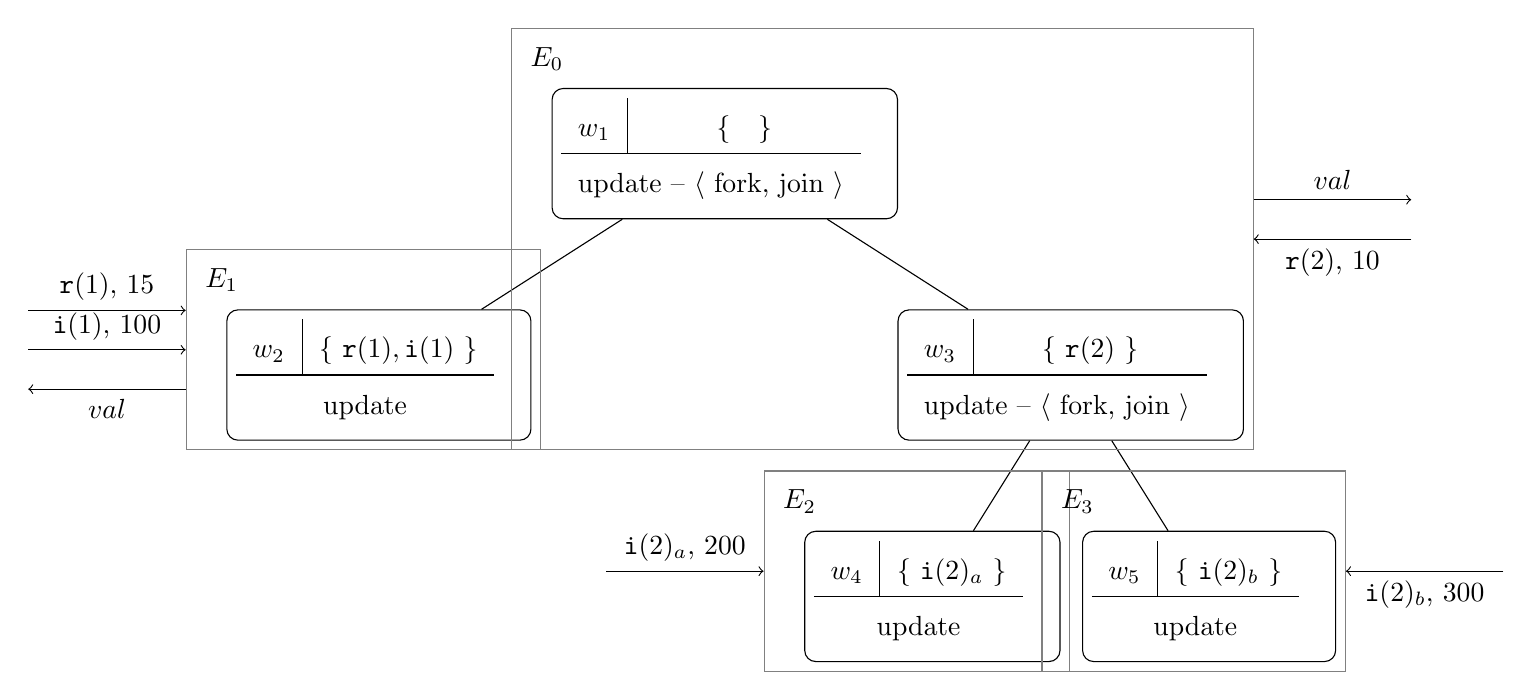
\begin{tikzpicture}[sibling distance=25em, level distance=80pt,
    every node/.style = {shape=rectangle,
      rounded corners,
      draw, align=center},
    level 1/.style = {sibling distance=25em},
    level 2/.style = {sibling distance=10em}]]

    \node (e0) { \TopDNode{$w_1$}{ }
                          {$E_0$}{update -- $\langle$ fork, join $\rangle$} }
      child { \DNode{$w_2$}{$\tg{r}(1), \tg{i}(1)$}{$E_1$}{update}{e1} }
      child { \DNode{$w_3$}{$\tg{r}(2)$}{$E_0$}{update -- $\langle$ fork, join $\rangle$}{e23}
          child { \DNode{$w_4$}{$\tg{i}(2)_a$}{$E_2$}{update}{e2} }
          child { \DNode{$w_5$}{$\tg{i}(2)_b$}{$E_3$}{update}{e3} } };

      %% Make the nodes
      \node (node0) [above=1mm of e0.north west, draw=none] { $E_0$ };
      \node [draw=black!50, fit={(e0) (e23) (node0)}, rounded corners=0] (c0) {};

      \node (node1) [above=1mm of e1.north west, draw=none] { $E_1$ };
      \node [draw=black!50, fit={(e1) (node1)}, rounded corners=0] (c1) {};

      \node (node2) [above=1mm of e2.north west, draw=none] { $E_2$ };
      \node [draw=black!50, fit={(e2) (node2)}, rounded corners=0] (c2) {};

      \node (node3) [above=1mm of e3.north west, draw=none] { $E_3$ };
      \node [draw=black!50, fit={(e3) (node3)}, rounded corners=0] (c3) {};

      %% Input streams

      \coordinate[right=20mm of c0] (d0);
      \coordinate[above=5mm of d0] (dd0);
      \coordinate[above=5mm of c0.east] (dc0);
      \draw [->] (d0) to[left] node[draw=none, auto] {$\tg{r}(2)$, 10} (c0);
      \draw [->] (dc0) to[right] node[draw=none, auto] {$val$} (dd0);

      \coordinate[left=20mm of c1] (d1);
      \coordinate[above=5mm of d1] (dd1);
      \coordinate[above=5mm of c1.west] (dc1);
      \coordinate[below=5mm of d1] (dd2);
      \coordinate[below=5mm of c1.west] (dc2);
      \draw [->] (d1) to[right] node[draw=none, auto] {$\tg{i}(1)$, 100} (c1);
      \draw [->] (dd1) to[right] node[draw=none, auto] {$\tg{r}(1)$, 15} (dc1);
      \draw [->] (dc2) to[left] node[draw=none, auto] {$val$} (dd2);

      \coordinate[left=20mm of c2] (d2);
      \draw [->] (d2) to[left] node[draw=none, auto] {$\tg{i}(2)_a$, 200} (c2);

      \coordinate[right=20mm of c3] (d3);
      \draw [->] (d3) to[right] node[draw=none, auto] {$\tg{i}(2)_b$, 300} (c3);

  \end{tikzpicture}}
  \caption{Example distributed implementation generated in \Cref{example:optimization}.
  The large gray rectangles $E_0$, $E_1$, $E_2$, $E_3$ represent physical nodes
  and the incoming arrows represent input streams and their relative rates.}
  \label{fig:distr_arch}
\end{figure}

\subsubsection{Implementation}
\label{ssec:runtime}

%% \str
%% \kk{The name of the subsubsection could be better.}
%%
Each node of the synchronization plan can be separated into two
components: an event processing component that is responsible for
computation via executing \fl{update},
\fl{fork}, and \fl{join} calls; and a mailbox
component that is responsible for enforcing ordering requirements and
synchronization.


\paragraph{Event Processing}
%
The worker processes execute the \fl{update},
\fl{fork}, and \fl{join} functions associated
with the tree node.  Whenever a worker is handed a message
by its mailbox, it first checks if it has any active children, and if
so, it sends them a join request and waits until it receives their
responses. After receiving these responses, it executes the join
function to combine their states, executes the update function on the
received event, and then executes the fork function on the new state,
and sends the resulting states to its children. In contrast, a leaf
worker just executes the update function on the received
event.

% \kk{Should we have an example here? Is this clear?}
% \caleb{Everything is better with an example. I think the example distribution plan (Figure~\ref{fig:example-configuration}) should be used throughout this section}

% \kk{This is the example of an execution. It should either be moved to distribution plans (simplified) or after the mailbox maybe?}

% For example, \Cref{fig:distr_arch}, shows a possible distribution of worker processes in a distributed
% architecture consisting of 4 physical nodes, $E_0$, $E_1$, $E_2$, and $E_3$, each one receiving streams of different
% implementation tags. Given that the mailboxes order incoming messages based on the dependency relation, leaf worker processes ($Worker_1$, $Worker_2$, $Worker_3$) concurrently process independent messages ($i_1$, $i_2$, $i_3$ respectively). Note that messages $d_1, d_2, d_3$ are processed by $Worker_0$ even though they arrive at the other nodes, because they are not independent from $i$ messages.

% As an example, suppose that a message with tag $\#$ with timestamp $10$ arrives at node $E_0$. $Worker_0$ would issue a join request with timestamp $10$ to all its descendants ($Worker_1$, $Worker_2$, $Worker_3$, $PhantomWorker_{23}$), who will process it after processing all messages that depend on $\#$ with smaller timestamps first. Then $PhantomWorker_{23}$ would join the states received by $Worker_2$ and $Worker_3$, and $Worker_0$ would join the states received by $Worker_1$ and $PhantomWorker_{23}$. $Worker_0$ would then run the update function on the message $\#$ and then it would fork back the newly updated state. Note that messages exchanged between workers in the same physical node (such as $Worker_0$ and $PhantomWorker_{23}$), are implemented as copy operations, and thus do not incur any overhead.

% If the example message sequence \tg{$d_1$}, \tg{$i_2$}, \tg{$i_3$}, \tg{$d_3$}, \tg{$\#$}  Node1 receives x, Node2 receives y, Node3 receives z. (\TODO{We have to adjust this to an example from section 2 or 3}. Describe what would happen in the implementation if a sequence of messages arrive (Do that for a sequence of messages that was introduced as an example in Section 2 or 3)

\paragraph{Event Reordering}
%
The mailbox of each worker ensures that it processes incoming
dependent events in the correct order by implementing the following
selective reordering procedure. Each mailbox contains an event buffer
and a timer for each implementation tag. The buffer holds the events
of a specific tag in increasing order of timestamps and the timer
indicates the latest timestamp that has been encountered for each tag.
When a mailbox receives an event $\langle \sigma, ts, v \rangle$ (or a
join request), it follows the procedure described below. It first
inserts it in the corresponding buffer and updates the timer for
$\sigma$ to the new timestamp $ts$. It then initiates a
cascading process of releasing events with tags $\sigma'$ that depend
on $\sigma$. During that process all dependent tags $\sigma'$ are
added to a dependent tag workset, and the buffer of each tag in the
workset is checked for potential events to release. An event $e =
\langle \sigma, ts, v \rangle$ can be released to the worker process
if two conditions hold. The timers of its dependent tags are higher
than the timestamp $ts$ of the event (which means that the mailbox has
already seen all dependent events up to $ts$, making it safe to
release $e$), and the earliest event in each buffer that $\sigma$
depends on should have a timestamp $ts' > ts$ (so that events are
processed in order). Whenever an event with tag $\sigma$ is released,
all its dependent tags are added to the workset and this process
recurses until the tag workset is empty.

\paragraph{Heartbeats}
\label{ssec:heartbeats}
As discussed in \cref{ssec:distributed-assumptions}, a dependence
between two implementation tags $\sigma_1$ and $\sigma_2$ requires the
implementation to process any event $\langle \sigma_1, t_i, v_i
\rangle$ after processing all events $\langle \sigma_2, t_j, v_j
\rangle$ with $t_j \leq t_i$. However, with the current assumptions on
the input streams, a mailbox has to wait until it receives the
earliest event $\langle \sigma_2, t_j, v_j \rangle$ with $t_j > t_i$,
which could arbitrarily delay event processing. We address this issue
with \emph{heartbeat} events, which are system events that represent
the absence of events on a stream.  These are commonly used in other
systems under different names, e.g.  heartbeats~\cite{heartbeats2005},
punctuation~\cite{punctuation2003},
watermarks~\cite{Flink2015}, or
pulses~\cite{schneider2013safe}.
% \str
% \kk{Rajeev mentions that these are not the same and we should discuss them in detail in the related work.}
Heartbeats are generated
periodically by the stream producers, and are interleaved together
with standard events of input streams.  When a heartbeat event
$\langle \sigma, t \rangle$ first enters the system, it is broadcast
to all the worker processes that are descendants of the worker that is
responsible for tag $\sigma$.  Each mailbox that receives the
heartbeat updates its timers and clears its buffers as if it has
received an event of $\langle \sigma, t, v \rangle$ without adding the
heartbeat to the buffer to be released to the worker process.

The latency (and overall performance) of the system directly depends on the rate of heartbeats for each tag.
More precisely, the latency associated with an event cannot be lower than the period ($1/{\text{rate}}$) of all the streams that it depends on. However,
higher hearbeat rates also negatively affect throughput and network load.
% (c.f. \Cref{sec:evaluation}) and network load
% (c.f. \Cref{ssec:latency-eval}).
 % there is a tradeoff between latency and network load, as the higher the heartbeat rate, the more events are sent over the network. We report on the tension between latency and network load related to heartbeat rates in \Cref{ssec:latency-eval}.
% \TODO{Bring that from appendix and reference}

% In order to prevent this from happening, \name{} uses heartbeat messages, which are a form of punctuation, and are used to indicate that an input stream is not "dead" (hence the name heartbeat), but rather that no message has arrived until a specific point in time.
% Heartbeats are very similar in nature to pulses \cite{mannermaa1999timing-gps, li2010deadlock, schneider2015safeparallelism}, which are another form of punctuation that is used to maintain a steady flow of messages throughout the system, therefore limiting the memory needed by message buffers.
% (\TODO{Find and cite punctuation literature. A good place to start might be the Safe Data parallelism for general streaming paper. In this paper, they define pulses, which are very similar to our heartbeats. They are forwarded by every operator in the system, and they limit the memory requirements of the system as well as prevent deadlock (in the case of bounded size buffers). Cite \cite{li2010deadlock, schneider2015safeparallelism} and argue about their use.})
% Heartbeats messages are of the form $\langle tag, timestamp \rangle$ and are interleaved together with standard messages in input streams.

\subsubsection{Proof of Correctness}
\label{ssec:proof-of-correctness}

We show that \emph{any} implementation produced by the end-to-end
framework is correct according to the semantics of the programming model.
First, \Cref{def:valid-input-instance} formalizes the
assumptions about the input streams outlined in
\Cref{ssec:distributed-assumptions}, and \Cref{def:distr-correctness}
defines what it means for an implementation to be correct with respect
to a sequential specification.  Our definition is inspired by the
classical definitions of distributed correctness based on
observational trace semantics (e.g.,~\cite{lynch1996distributed}).
However, we focus on how to interpret the independent input streams as
a sequential input, in order to model possibly synchronizing and
order-dependent stream processing computations.

\begin{definition}
\label{def:valid-input-instance}
A \emph{valid input instance} consists of
$k$ input streams (finite sequences) \fl{u_1}, \fl{u_2}, \ldots{}, \fl{u_k} of type \fl{List(Event |} \fl{Heartbeat)},
and an order relation $\mathcal{O}$ on input events and heartbeats, with the following properties.
(1) \emph{Monotonicity:} for all $i$, \fl{u_i} is in strictly increasing order according to $\mathrel{<_{\mathcal{O}}}$.
(2) \emph{Progress:} for all $i$, for each input event (non-heartbeat) \fl{x} in \fl{u_i},
for every other stream $j$ there exists an event or heartbeat \fl{y} in \fl{u_j} such that ${\fl{x}} \mathrel{<_{\mathcal{O}}} {\fl{y}}$.
\end{definition}

\noindent
Given a DGS specification $S$,
the \emph{sequential specification} is a function \fl{spec:} \fl{List(Event) -> List(Out)},
obtained by applying only \fl{update}
functions and no \fl{fork} and \fl{join} calls.
The output specified by \fl{spec} is produced incrementally (or \emph{monotonically}): if \fl{u} is a prefix of \fl{u'}, then \fl{spec(u)} is a subset of \fl{spec(u')}.
Define the \emph{sort} function
${\fl{sort}}_{\mathcal{O}}:$ \fl{List(List(Event |} \fl{Heartbeat)) ->} \fl{List(Event)}
which takes $k$ sorted input event streams and sorts them
into one sequential stream, according to the total order relation $\mathcal{O}$, and drops heartbeat events.

\begin{definition}
\label{def:distr-correctness}
Given a sequential specification \fl{spec:} \fl{List(Event) ->} \fl{List(Out)},
a distributed implementation is \emph{correct} with respect to \fl{spec} if for every valid input instance $\mathcal{O}$, \fl{u_1}, \ldots, \fl{u_k},
the set of outputs produced by the implementation is equal to
${\fl{set}(\fl{spec}}({\fl{sort}}_{\mathcal{O}}({\fl{u_1}}, \ldots, {\fl{u_k}})))$.
\end{definition}

\noindent
We show that our framework is correct according to \Cref{def:distr-correctness}.
% \Cref{theorem:correctness} in \Cref{sec:appendix-proof-of-correctness}
% formally states that our framework is correct according to
% \Cref{def:distr-correctness}.
The key assumptions used are:
\begin{enumerate}
\item[(1)] The specification given by the programmer is consistent, as defined in \Cref{ssec:prog-model-correctness}.
\item[(2)] The input streams constitute a valid input instance, as defined in \Cref{def:valid-input-instance}.
\item[(3)] The synchronization plan that is chosen by the optimizer is valid, as defined in \Cref{ssec:distributed-configurations}.
\item[(4)] Messages that are sent between two processes in the system arrive in order and are always received. This last assumption is ensured by the Erlang runtime.
% \item[(5)] The underlying scheduler is fair, i.e. all processes get scheduled infinitely often.
\end{enumerate}

The proof decomposes the implementation into the mailbox
implementations and the worker implementations, which are both sets of
processes that given a set of input streams produce a set of output
streams. We first show that the mailboxes transform a valid input
instance to a worker input that is correct up to reordering of
independent events. Then we show that given a valid worker input, the
workers processes' collective output is correct.
The second step relies on
\Cref{thm:consistency-implies-determinism},
from the previous section, as well as
\Cref{lemma:worker-wire-correspondence}
which ties this to the mailbox implementations,
showing that the implementation produces a valid wire diagram according to the formal semantics of the specification $S$.
Given a valid input instance $u$ and a computation specification $S$ that contains
in particular a sequential specification \fl{spec: List(Event) -> List(Out)},
  % a set of specification tags \fl{Tag},
  % a dependence relation \fl{dependencies},
  % and parallelization primitives,
we want to show that any implementation $f$ that is produced by our framework is correct according to \Cref{def:distr-correctness}.

\begin{definition}
For a valid input instance $u$, a worker input $m_u = (m_1, ..., m_N)$
is \emph{valid} with respect to $u$ if $m_i \in \mathrm{reorder}_{D_I}
(\mathrm{filter}(\mathrm{rec}_{w_i}, \mathrm{sort}_O(u))),$ where
$\mathrm{reorder}_{D_I}$ is the set of reorderings that preserve the
order of dependent events,
  $\mathrm{rec}_w(\langle \sigma, t, p\rangle) = \sigma \in \mathrm{atags}(w) \cup \wfield{w}{itags}$
  is a predicate of the messages that each worker $w$ receives,
  and $\mathrm{atags}$ is the set of implementation tags that are handled by a workers ancestors, and is given by $\mathrm{atags}_w = \{ \wfield{w'}{itags} : \forall w' \in \mathrm{anc}(w', w)\}$.
\end{definition}

\begin{lemma}
\label{lemma:mailbox}
Given a valid input instance $u$, any worker input $m$ produced by
the mailbox implementations $(u, m)$ in $f$ is valid with respect to
$u$.
\end{lemma}
\begin{proof}
By induction on the input events of one mailbox and using assumptions
(2)-(4).
\end{proof}

Each worker $w$ runs the update function on each event $e = \langle
\sigma, t, p\rangle$ on its stream that it is responsible for $\sigma
\in \wfield{w}{itags}$ possibly producing output $\fl{o: List(Out)}$.
For all events in the stream that one of its
ancestors is responsible for, it sends its state to its parent worker
and waits until it receives an updated one.
The following key lemma states that this corresponds to a particular
wire diagram in the semantics of the specification.

\begin{lemma}
\label{lemma:worker-wire-correspondence}
Let $m$ be the worker input to $f$ for specification $S$
on input \fl{u},
and let $\fl{o}_i: \fl{List(Out)}$ be the stream of output events
produced by worker $i$ on input $m_i$.
Then there exists \fl{v: List(Out)}
such that $\fl{inter}(\fl{v}, \fl{o}_1, \fl{o}_2, \ldots, \fl{o}_N)$
and $(\fl{u}, \fl{v}) \in \sem{S}$.
\end{lemma}
\begin{proof}
By induction on the worker input and using assumption (3), in particular
validity condition (V1),
we first show that the worker input corresponds to a wire diagram,
in particular we show that
$\semantics{\fl{State_0}}{\fl{true}}{\fl{s}}{\fl{u}'}{\fl{s'}}{\fl{v}}$
where \fl{v} is an interleaving of $\fl{o}_1, \ldots, \fl{o}_N$
and $\fl{u}'$ is \emph{any} interleaving of the events
$\fl{u}'_i$
processed by each mailbox, namely
$\mathrm{filter}(\mathrm{rec}_{w_i}, \wfield{w_i}{itags})$.
Applying \cref{lemma:mailbox},
\fl{u} is one possible interleaving of the events $\fl{u}'_i$
and hence we conclude that
$\semantics{\fl{State_0}}{\fl{true}}{\fl{s}}{\fl{u}}{\fl{s'}}{\fl{v}}$,
thus
$(\fl{u}, \fl{v}) \in \sem{S}$.
\end{proof}

%% No longer needed, only matters if output order is
% important
% denoted as $e
% \rightsquigarrow o$.

% \begin{definition}
% Given a valid worker input instance $m_u$, the output partial order
% $z_u$ produced by the workers contains all the events $o$ that
% $\forall e \in m_u, e \rightsquigarrow o$. Two output events are
% ordered $o_1 < o_2$, if $e_1 \rightsquigarrow o_1$, $e_2
% \rightsquigarrow o_2$, and $e_1 < e_2$ in the same worker input stream
% $e_1, e_2 \in m_i$.
% \end{definition}

% \kk{There is a small issue, but I don't know how crucial it is and whether we should mention it. The parent node indeed runs the update (thus producing output) before the childre nodes. However, since the output is sent to a sink by all workers, the children output might arrive first, even if it was produced second. The way to solve it would be to introduce some system metadata in the output events, maybe in the form of logical timestamps (like vector timestamps). Then the sink could order the output events according to logical timestamp and then pass them on.}
% \caleb{Oh I see, this seems like a problem. Maybe we should say our current implementation just assumes output is totally unordered?}
% \kk{Address this issue by mentioning that the output partial order is determined either by timestamps, or by the time a message was processed in an update function. A tree of logical vector clocks is probably enough to order different events. More precisely, a path in a tree is enough, and two events can only be ordered up to the point that they share a path prefix}

% \begin{lemma}
% \label{lemma:output}
% For all pairs of output events $o_1, o_2$ produced by a valid worker
% input instance, if $e_1 \rightsquigarrow o_1$, $e_2 \rightsquigarrow
% o_2$, $e_1 <_O e_2$, and $e_1 D e_2$, then $o_1 < o_2$.
% \end{lemma}

% \begin{proof}
% If $e_1 D e_2$, there exists a leaf worker input $m_i$ such that
% $e_1, e_2 \in m_i$, by assumption (3).
% \end{proof}

% \begin{lemma}
% \label{lemma:workers}
% For all $u$, for every worker inputs $m_u$ that is valid with respect
% to $u$, and for every worker output partial order $z_u$ produced by a
% valid worker input $m_u$, there exists a total order extension $v$ of
% $z_u$, such that $\left( \pi(\mathrm{sort}_O(u)), v \right) \in
% \varphi$.
% \end{lemma}
% \begin{proof}
% By induction on the worker inputs and using \Cref{lemma:output}
% and assumptions (1) and (3).
% \end{proof}

Combining \Cref{lemma:worker-wire-correspondence}
and \Cref{thm:consistency-implies-determinism} then yields the end-to-end correctness theorem.

\begin{theorem}[Implementation Correctness]
\label{theorem:correctness}
$f$ is correct according to \cref{def:distr-correctness}.
\end{theorem}

% \begin{proof}
% We know that for all $(u, v) \in f$, there exists $m_u$ which is valid
% with respect to $u$ such that $(u, m_u)$ is a mailbox in $f$.
% By \Cref{lemma:worker-wire-correspondence},

% f_w$. By Lemmas~\ref{lemma:mailbox} and~\ref{lemma:workers}, we know
% that for every worker output $z_u$, there exists a total order
% extension $v$ of $z_u$, such that $\left( \pi(\mathrm{sort}_O(u)), v
% \right) \in \varphi$.
% \end{proof}

\subsection{Evaluation}

We show some highlights from the evaluation of DGS
in \Cref{fig:existing-implementations-scaling},
\Cref{fig:timely-snippet},
% \Cref{fig:synchronization-plan-fraud-detection-throughput},
\Cref{fig:synchronization-plan-throughputs-flink},
and \Cref{fig:flumina-scaling}.

\begin{figure}[t]
    \centering
    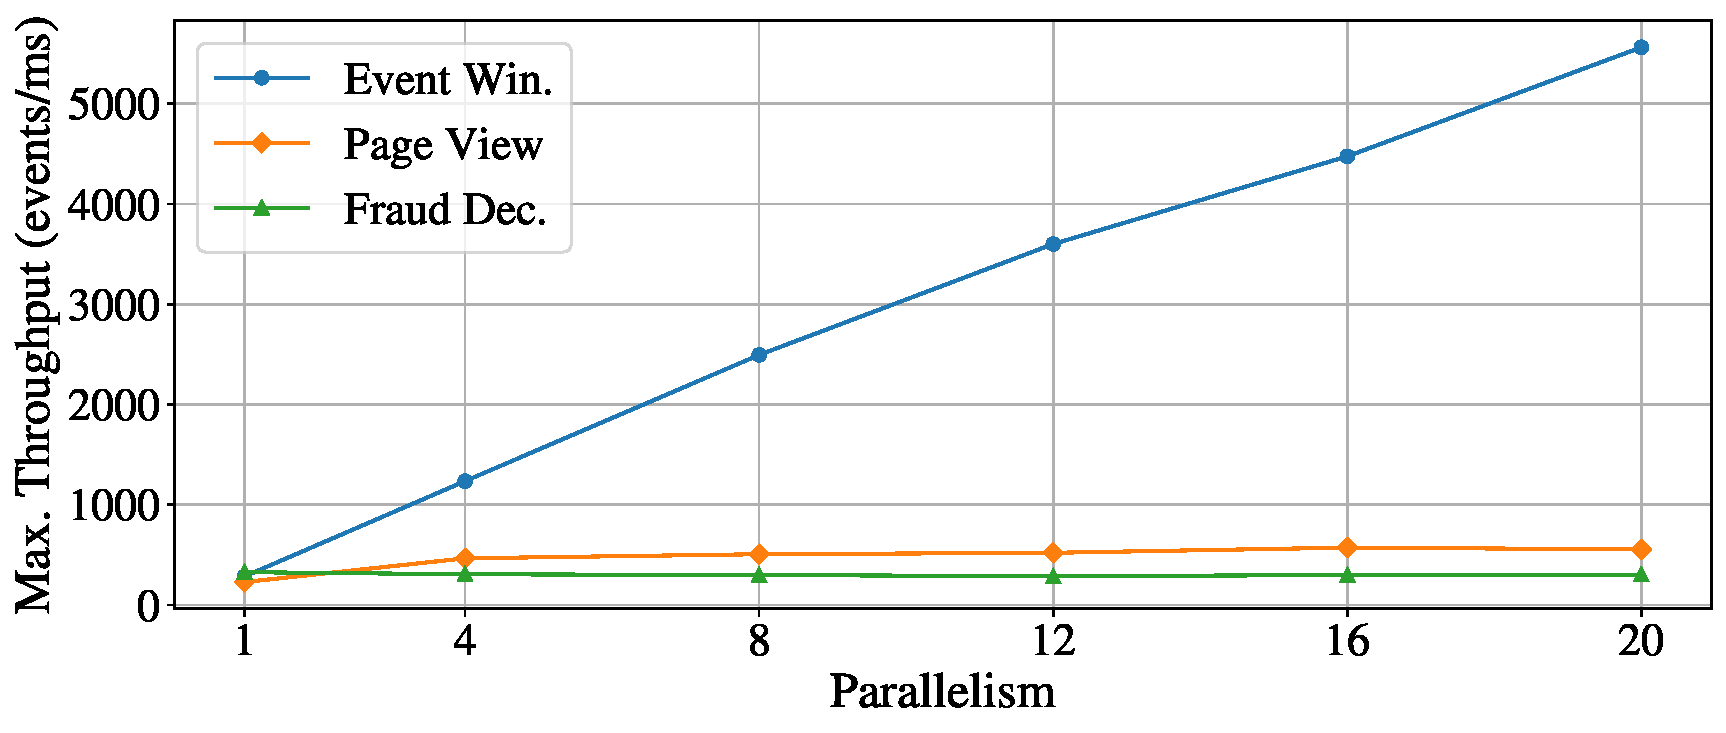
\includegraphics[width=0.48\columnwidth]{figures/dgs/flink_max_throughput_scaleup}
    ~
	  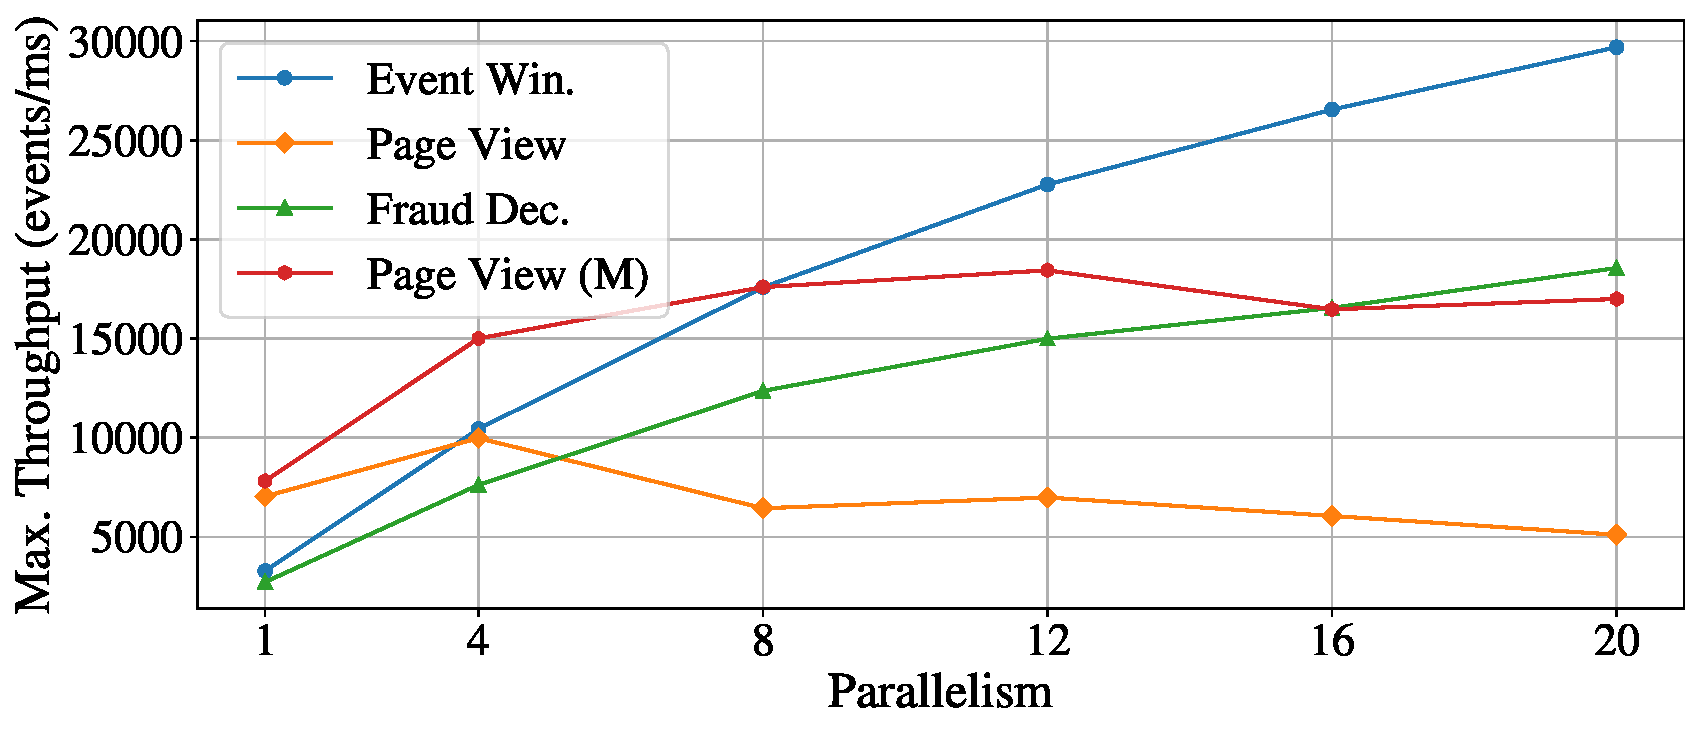
\includegraphics[width=0.48\columnwidth]{figures/dgs/timely_max_throughput_scaleup}
    \caption{
    Flink (left) and Timely (right) implementations maximum throughput increase with increasing parallel nodes for the three applications that require synchronization.
	% \caleb{Can we put these side by side? The figure is not very aesthetically pleasing right now.}
  % \kk{It is true that it is not pleasing, but putting them side by side will make the fonts too small.}
    % \kk{Include more summarization numbers in the prose.}
	% \str
	% \caleb{todo Konstantinos: can you remove the manual from Timely?}
    }
    \label{fig:existing-implementations-scaling}
\end{figure}


\begin{figure}[t]
  \centering
  \footnotesize{}
\begin{verbatim}
updates.broadcast().filter(move |x| {
    x.name == page_partition_function(NUM_PAGES, worker_index)
});
\end{verbatim}
\caption{Snippet of the manual (M) Timely implementation of the Page View example.
This violates \textbf{PIP2} since it explicitly references the physical partitioning of input streams
(\texttt{page\_partition\_function}) and the index of the worker that processes each stream (\texttt{worker\_index}).
}
\label{fig:timely-snippet}
\end{figure}


\begin{figure}[t]
    \centering
    \begin{subfigure}[b]{0.35\textwidth}
      \centering
      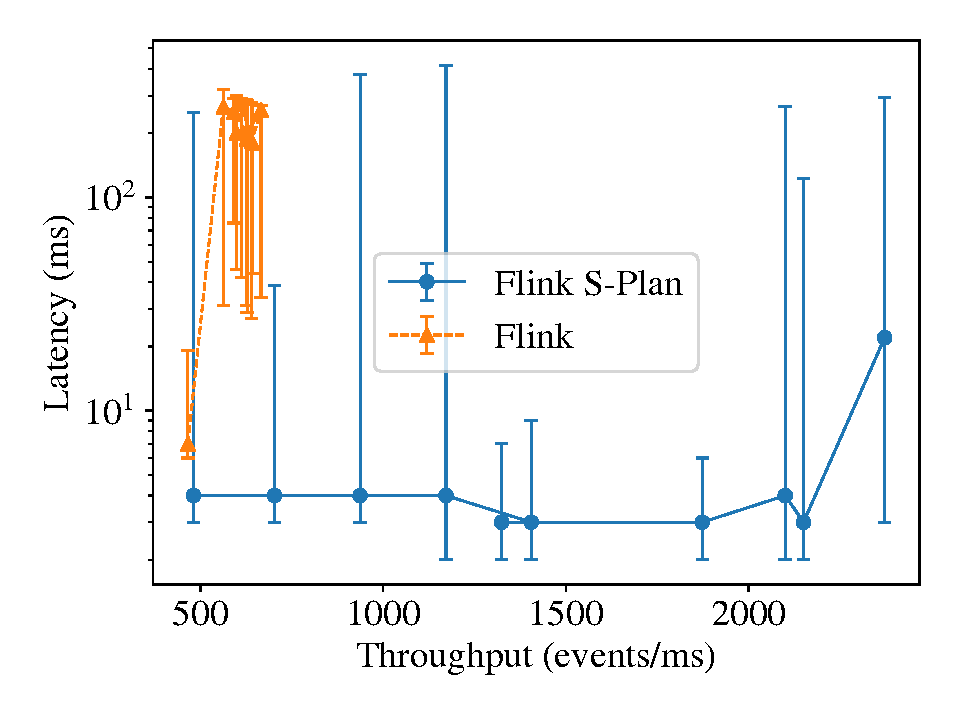
\includegraphics[width=\textwidth]{figures/dgs/pageview-flink-splan.pdf}
      \caption{Page-view Join.}
      \label{fig:synchronization-plan-page-view-join-throughput}
    \end{subfigure}
    \hspace{0.05\textwidth}
    \begin{subfigure}[b]{0.35\textwidth}
      \centering
      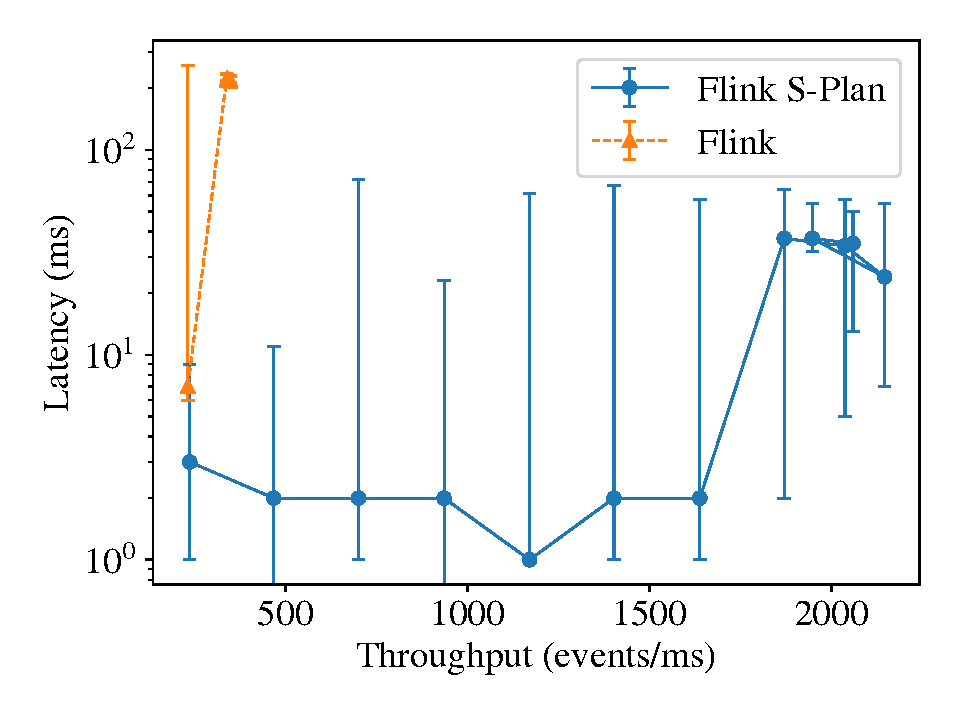
\includegraphics[width=\textwidth]{figures/dgs/frauds-flink-splan.pdf}
      \caption{Fraud Detection.
    %   Input rates from \todo{X} to \todo{Y}.
    %   \todo{12} nodes.
      }
      \label{fig:synchronization-plan-fraud-detection-throughput}
    \end{subfigure}
    \caption{
      Throughput (x-axis) and 10th, 50th, 90th percentile latencies on the y-axis for increasing input rates (from left to right) and 12 parallel nodes. Flink represents the parallel implementation produced automatically, and Flink S-Plan represents the synchronization plan implementation.
      }
    \label{fig:synchronization-plan-throughputs-flink}
\end{figure}

\begin{figure}
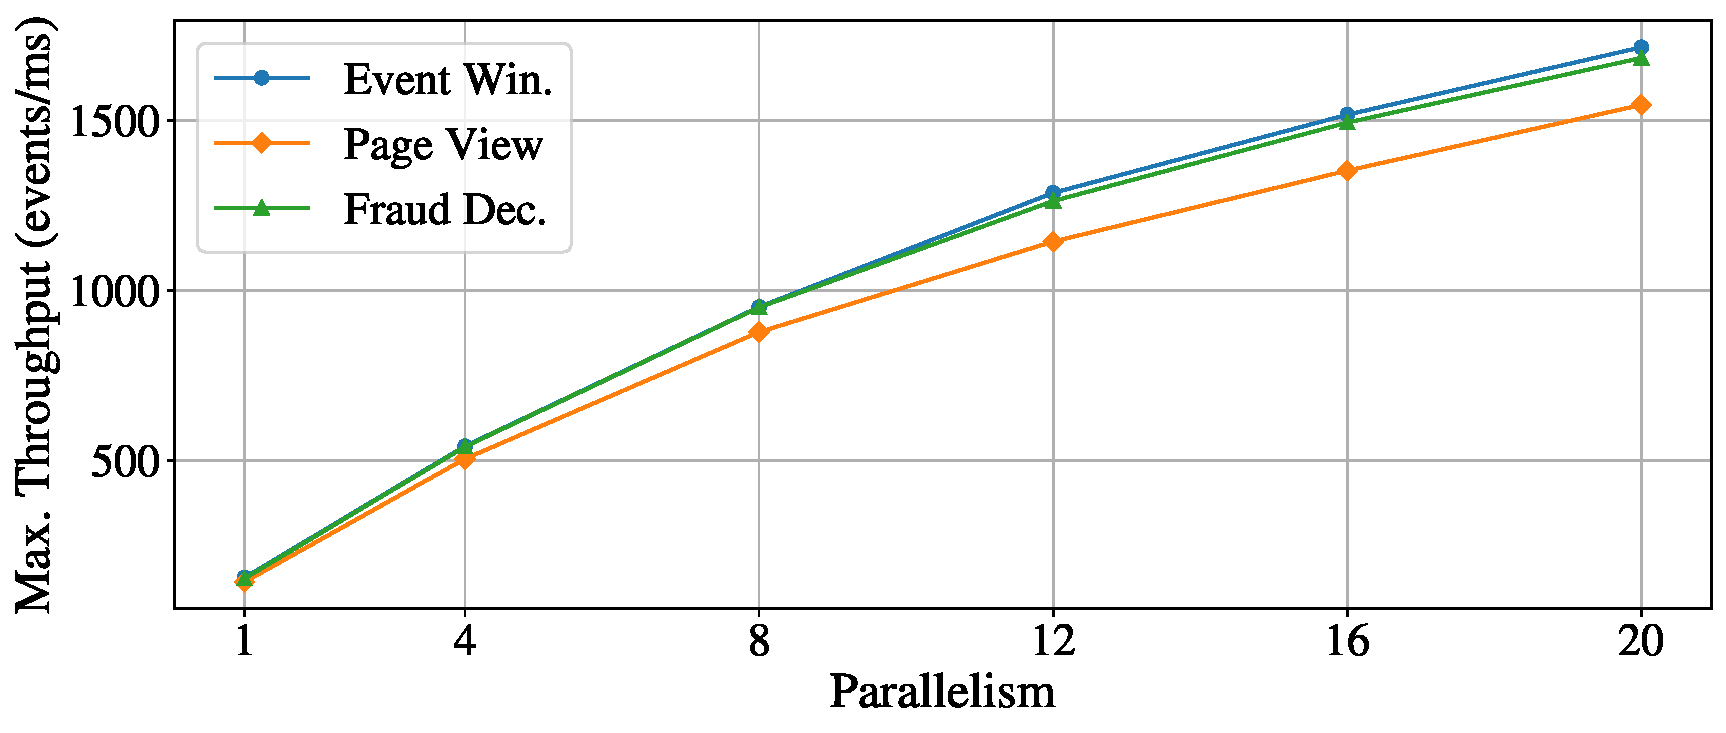
\includegraphics[width=\linewidth]{figures/dgs/flumina_max_throughput_scaleup.pdf}
\captionof{figure}{
DGSStream maximum throughput increase with increasing parallel nodes for the three applications that require synchronization.}
\label{fig:flumina-scaling}
\end{figure}

\chapter{Testing}
\label{cha:testing}
\headerblock{
  \headerquote{The return on investment from random testing is good. Our rough
  estimate—including faculty, staff, and student salaries, machines
  purchased, and university overhead—is that each of the more than
  325 bugs we reported cost less than \$1,000 to find.}{Yang, Chen, Eide, and Regehr, 2011~\cite{yang2011finding}}
}

Given the typing discipline in \Cref{cha:foundation}, \Cref{cha:composition,cha:distribution} have considered ways to write well-typed programs: programs defined compositionally, and for which they can be parallelized in a semantics-preserving way that ensures determinism.

This section considers the problem from a different angle: suppose we have an application that is already defined, or an input arriving from an external source; can we \emph{test} empirically whether it is well-typed and deterministic with respect to a given input and output stream type?
This problem is not easy. One issue is that the property we are interested in can be thought of as ``on all executions, the ordering of the stream is the same up to equivalence'' which is a property that requires running the program multiple times (i.e. a ``hyperproperty'').
We consider \emph{differential testing} as a way to address this and test at runtime whether a program satisfies its stream typing requirements.

Specifically, we consider differential testing of two output streams, up to equivalence defined by a stream type $S'$.
This may seem more restricted than testing whether a program is well-typed with input type $S$ and output type $S'$,
but it turns out to be only more specific in some aspects, and more general in others.
To solve the type safety and determinism problem, we have to generate two example inputs that are equivalent, feed them each to the same program $P$, and apply the differential testing algorithm on the two resulting outputs.
So if we also have an input generation procedure, then we can solve the general type safety and determinism problem.
But we can also apply differential output testing to two \emph{different} programs $P_1$ and $P_2$ (typically, a sequential version and a parallel version), which should be equivalent, and compare their outputs.

\section{Motivation}
\label{diffstream:sec:introduction}

Beyond the context of this thesis, the problem of ensuring correctness of distributed programs is long established, as can be seen by the significant amount of past and ongoing work on the correctness of distributed protocols (e.g., \cite{chand2016formal,abdulla2014optimal,padon2016ivy}), concurrent data structures (e.g., \cite{herlihy1990linearizability,burckhardt2014replicated}),
and distributed systems (e.g., \cite{ozkan2018randomized,wilcox2015verdi,hawblitzel2015ironfleet}).
In general, because this body of work addresses the challenges of verification of distributed protocols and low-level primitives, it targets experts who design and implement complex distributed systems.
However, data-parallel programming frameworks, such as stream processing systems, aim to offer a simplified view of distributed programming where low level coordination and protocols are hidden from the programmer. This has the advantage of bringing distributed programming to a wider audience of end-users, and at the same time it requires new tools that \emph{can be used by such end-users} (rather than just experts) to automatically test for correctness.

Unfortunately, there is limited work in testing for stream processing programs; in fact, the state of the art in practice is unit and integration testing~\cite{vianna2019exploratory}.
In order to bridge this gap and provide support for checking correctness to end-users,
we focus on the problem of \emph{differential  testing} for distributed stream processing systems, that is, checking whether the outputs produced by two implementations in response to an input stream are equivalent.
Differential testing~\cite{mckeeman1998differential,groce2007randomized,evans2007differential},
allows for a simple specification of the correct program behavior, in contrast to more primitive testing techniques, where
the specification is either very coarse (i.e. the application doesn't crash) or very limited (i.e. on a given input, the application should produce a specific output).
More precisely, differential testing allows for a reference implementation to be the specification. This is especially useful in the context of distributed stream processing systems, since bugs introduced due to distribution can be caught by comparing a sequential and a distributed implementation. In addition, having a reference implementation as a specification allows testing with random inputs, since there is no need to specify the expected output.

We identify two critical challenges in testing stream processing programs.
The first challenge is dealing with output events that are out-of-order due to parallelism. In particular, for differential testing,
two implementations might produce events at different rates, asynchronously, and out-of-order.
However, the order between specific output events might not affect the downstream consumer (e.g. events with timestamp less than $t$ can arrive in any order, as long as they arrive before the watermark $t$),
therefore requiring our notion of equivalent streams which allows for out-of-order events.
In fact, lack of order is often desirable, since it enables parallelism.
Importantly on the other hand, \emph{not all} output events are unordered, because operators in streaming dataflow graphs (in contrast to in batch processing and MapReduce settings) often require some order to preserved (see \Cref{diffstream:sec:overview}).
Because of this, not all operators simply decompose into commutative/associative aggregators, and prior solutions on testing~\cite{csallner2011new,xu2013semantic,marynowski2012testing,chen2016commutativity} and static verification~\cite{liu2014automating,raychev2015parallelizing} for MapReduce-like programs cannot be directly applied.

The second challenge is that
stream processing systems, in contrast to batch processing systems,
are designed to process input data that would not fit
in memory.  As best practice, it is recommended that applications written in these systems are
tested under heavy load for long periods of time, to match the
conditions that are expected after
deployment~\cite{vianna2019exploratory}. Achieving this requires that
the testing framework itself is an online algorithm, in the sense that
it processes output events as they arrive, and that the computational overhead is minimal.

\section{Contributions}

We propose a matching algorithm that incrementally compares two streams for equivalence.
Following the approach of \citeMain{pldi19}, in our solution, ordering requirements between pairs of events are abstracted in a \emph{dependence relation} that indicates when the ordering of two specific events is of significance to the output consumer.
Given \emph{any} dependence relation provided by the user, the algorithm determines, in an online fashion, whether the streams are equivalent up to the reorderings allowed by the dependence relation.
We show that the algorithm is correct and that it reaches a negative verdict at the earliest possible time (\Cref{diffstream:thm:correctness}).
We also prove that the algorithm is optimal, in the sense that it uses a minimal amount of space: any correct online algorithm must store at least as much information (\Cref{diffstream:thm:optimality}).

We have implemented DiffStream{}, a differential testing library for Apache Flink that incorporates our algorithm.
DiffStream{} is implemented in Java and can be used alongside existing
testing frameworks such as
JUnit~\cite{JUnitWeb} or in stand-alone Flink programs.
In order to evaluate the effectiveness and usability of the proposed testing framework, we have conducted a series of case studies.

First, we evaluate the effectiveness of the framework on a
set of nondeterministic MapReduce programs from \cite{xiao2014nondeterminism}, adapted to the streaming setting.
For some of these programs nondeterminism constitutes a bug, while for others it is acceptable, depending on input assumptions and application requirements.
Using our framework, we demonstrate that tests can be written to successfully detect 5 out of 5 bugs (true positives), and to avoid flagging 5 out of 7 bug-free programs (false positives).
This improves on previous work~\cite{xu2013testing}, which would generally flag all nondeterministic programs as buggy, thus suffering from false positives.

Second, we design two specific use cases to illustrate the benefits of
using DiffStream to design and implement parallel Flink applications. We
consider a difficult-to-parallelize application which requires
event-based windowing: we show that it is significantly more difficult
(requiring twice as many lines of code) to effectively parallelize
this application using Flink, and we show how our framework can be
used to test and correctly implement such an application. We also
evaluate the effort needed to write tests for an example computation
with a subtle bug. The specific programs we consider are explained in
more detail in \Cref{diffstream:sec:overview}.

Finally, we demonstrate that the matching algorithm is efficient in
practice, and can be used in an online monitoring setting, by
monitoring two implementations of the Yahoo Streaming
Benchmark~\cite{yahoostreaming2016} over the span of two hours and measuring the impact on performance.
The overhead of testing is a modest $5\%$ reduction in maximum possible throughput, and the memory usage remains stable at less than 500 unmatched items out of 30K items per second, reflecting the theoretical optimality of the algorithm for this particular application.

In total, the main contributions of this work are:
\begin{itemize}
    \item A new testing methodology for specifying ordering
      requirements in stream processing programs. (\Cref{diffstream:sec:dependence-relation})
    \item An optimal online matching algorithm for differential
      testing of stream processing programs which uniformly handles
      data with differing ordering requirements. (\Cref{diffstream:sec:algorithm})
    \item DiffStream, a differential testing library for testing Apache
      Flink applications based on the online matching algorithm, together with a series of case studies to evaluate its
        usability and effectiveness.
        (\Cref{diffstream:sec:evaluation})
\end{itemize}

DiffStream is available as an open-source repository \githubref{https://github.com/fniksic/diffstream}{on GitHub}.

\section{Example Use Cases}
\label{diffstream:ssec:motivating-examples}
\label{diffstream:sec:overview}

Programs written in distributed stream processing frameworks exhibit implicit parallelism, which can lead to subtle bugs. Programs in such frameworks are usually written as \emph{dataflow graphs}, where the edges are data streams and the nodes are streaming operators or transformations.
Common operators include stateless transformations (\emph{map}), and operations that group events based on the value of some field (\emph{key-by}).
For example, suppose that we have a single input stream which contains information about rides of a taxi service: each input event $(\texttt{id}, \texttt{pos}, \texttt{meta})$ consists of a taxi identifier, the taxi position, and some metadata. In the first stage, we want to discard the metadata component (\emph{map}) and partition the data by taxi ID (\emph{key-by}). In the second stage, we want to aggregate this data to report the total distance traveled by each taxi. Notice that the second stage is order-dependent (events for each taxi need to arrive in order), so it is important that the first stage does not disrupt the ordering of events for a particular taxi ID.

\begin{figure}[tb]
\centering
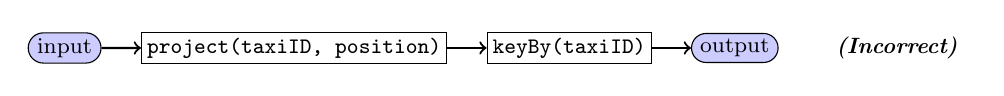
\begin{tikzpicture}[node distance=0.5cm,every node/.style={font=\footnotesize}]
\node[source] (in) {input};
\node[operator, right=of in] (op1) {\texttt{project(taxiID, position)}};
\node[operator, right=of op1] (op2) {\texttt{keyBy(taxiID)}};
\node[sink, right=of op2] (out) {output};
\node[right=of out,minimum width=2cm] (label) {\textbf{\emph{(Incorrect)}}};

\draw[dataflowedge] (in) -- (op1);
\draw[dataflowedge] (op1) -- (op2);
\draw[dataflowedge] (op2) -- (out);
\end{tikzpicture}

\smallskip

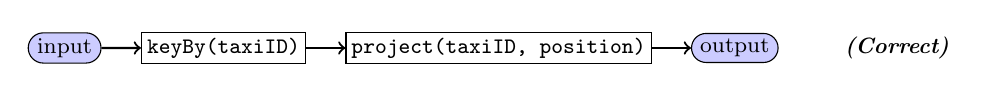
\begin{tikzpicture}[node distance=0.5cm,every node/.style={font=\footnotesize}]
\node[source] (in) {input};
\node[operator, right=of in] (op1) {\texttt{keyBy(taxiID)}};
\node[operator, right=of op1] (op2) {\texttt{project(taxiID, position)}};
\node[sink, right=of op2] (out) {output};
\node[right=of out,minimum width=2cm] (label) {\textbf{\emph{(Correct)}}};

\draw[dataflowedge] (in) -- (op1);
\draw[dataflowedge] (op1) -- (op2);
\draw[dataflowedge] (op2) -- (out);
\end{tikzpicture}

\caption[DiffStream example use case 1.]{A subtle consequence of implicit parallelism
over an input stream containing taxi location data.
}
\label{diffstream:ex:overview-simple}
\end{figure}

To make a program for the first stage of this computation in a distributed stream processing framework such as Flink or Storm, we need to build a dataflow graph representing a sequence of transformations on data streams. A first (natural) attempt to write the program is given in \Cref{diffstream:ex:overview-simple} (top). Here, the \texttt{project} node projects the data to only the fields we are interested in; in this case, \texttt{taxiID} and \texttt{position}. And \texttt{keyBy} (also known as ``group by'' in SQL-like languages, or the concept of a ``stream grouping'' in Storm) partitions the data stream into substreams by \texttt{taxiID}.
Although written as an operator, here \texttt{keyBy} can be thought of as modifying the stream to give it a certain property (namely, if it is parallelized, streams should be grouped by the given key).

The first attempt is incorrect, however, because it fails to preserve
the order of data for a particular key (taxi ID), which is required
for the second stage of the computation. The problem is that dataflow
graph operators are implicitly parallelized---here, the stateless map
\texttt{project} is internally replicated into several copies, and the
events of the input stream are divided among the copies.
Because input events of the same key may get split across substreams,
when the operator \texttt{keyBy} reassigns each item to a new
partition based on its key, if items of a particular key were
previously split up, then they might get reassembled in the wrong
order.

This issue can be addressed by ensuring that parallelization is done only on the basis of \texttt{taxiID} \emph{from the beginning of the pipeline}.
This can typically be accomplished by simply by reversing the \texttt{project} and \texttt{keyBy} transformations, as in \Cref{diffstream:ex:overview-simple} (bottom).
(For example, this is done explicitly in Flink, and the concept is the same in Storm, except that instead of an explicit \texttt{keyBy} operator we implicitly construct it by setting the input stream to be grouped by key.)
Although the two programs are equivalent when the \texttt{project} operation is not parallelized, the second lacks the undesirable behavior in the presence of parallelism: assuming the \texttt{project} operation has the same level of parallelism as \texttt{keyBy}, most systems will continue to use the same partition of the stream to compute the projection, so data for each key will be kept in-order. In particular, this works in any framework which guarantees that the same key-based partitioning is used between stages.

We have seen that even simple programs can exhibit counterintuitive behavior. In practice, programs written to exploit parallelism are often much more complex. To illustrate this, consider a single input stream consisting of very large documents, where we want to assign a topic to each document. The documents are streamed word by word and delineated by end-of-file markers.
The topic of each word is specified in a precomputed database, and the topic of a document is defined to be the most frequent topic among words in that document.

\begin{figure}[tb]
\centering
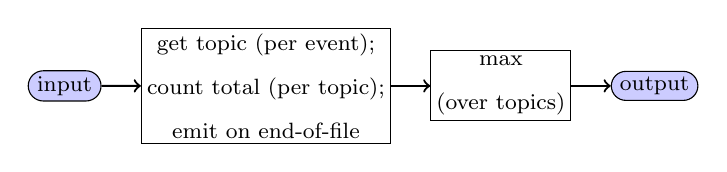
\begin{tikzpicture}[node distance=0.5cm,every node/.style={font=\footnotesize}]
\node[source] (in) {input};
\node[operator, right=of in] (op1) {get topic (per event); \\ count total (per topic); \\ emit on end-of-file};
\node[operator, right=of op1] (op2) {max \\ (over topics)};
\node[sink, right=of op2] (out) {output};

\draw[dataflowedge] (in) -- (op1);
\draw[dataflowedge] (op1) -- (op2);
\draw[dataflowedge] (op2) -- (out);
\end{tikzpicture}

\vspace{-2pt}

\rule{0.4\textwidth}{0.5pt}

\bigskip

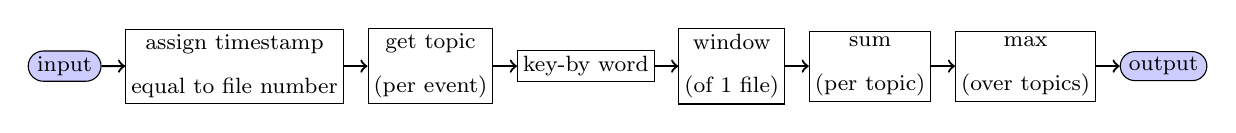
\begin{tikzpicture}[node distance=0.3cm,every node/.style={font=\footnotesize}]
\node[source] (in) {input};
\node[operator, right=of in] (op1) {assign timestamp \\ equal to file number};
\node[operator, right=of op1] (op2) {get topic \\ (per event)};
\node[operator, right=of op2] (op3) {key-by word};
\node[operator, right=of op3] (op4) {window \\ (of 1 file)};
\node[operator, right=of op4] (op5) {sum \\ (per topic)};
\node[operator, right=of op5] (op6) {max \\ (over topics)};
\node[sink, right=of op6] (out) {output};

\draw[dataflowedge] (in) -- (op1);
\draw[dataflowedge] (op1) -- (op2);
\draw[dataflowedge] (op2) -- (op3);
\draw[dataflowedge] (op3) -- (op4);
\draw[dataflowedge] (op4) -- (op5);
\draw[dataflowedge] (op5) -- (op6);
\draw[dataflowedge] (op6) -- (out);
\end{tikzpicture}

\caption[DiffStream example use case 2.]{A difficult-to-parallelize sequential program (top), and the correct parallel version (bottom)
over an input set of documents which arrive concatenated in a single stream.
}
\label{diffstream:ex:overview-complex}
\end{figure}

In this second example querying the database is a costly operation, so
it is desirable to parallelize by partitioning the words within each
document into substreams. However, the challenge is to do so in a way
that allows for the end-of-file markers to act as \emph{barriers}, so
that we re-group and output the summary at the end of each document.
Although a sequential solution for this problem is easy, the simplest
solution we have found in Flink that exploits parallelism uses about
twice as many lines of code
(\Cref{diffstream:ex:overview-complex}).
The source of the complexity is that we must first use the end-of-file events to assign a unique timestamp to each document (ignoring the usual timestamps on events used by Flink). After these timestamps are assigned, only then is it safe to parallelize, because windowing by timestamp later recovers the original file (set of events with a given timestamp).
We also consulted with Flink users
on the Flink mailing list, and we were not able to come up with a
simpler solution.
% This example is explored in detail in
% \Cref{diffstream:ssec:evaluation-wordcount}.
The additional complexity in
developing the parallel solution, which requires changing the dataflow
structure and not simply tuning some parameter, further motivates the
need for differential testing.

\section{DiffStream}
\label{diffstream:ssec:overview-solution}

These examples motivate the need for some form of testing to determine
the correctness of distributed stream processing applications. We propose \emph{differential testing} of the sequential and parallel versions. As the parallel solution might be much more involved, this helps validate that parallelization was done correctly and did not introduce bugs.

In the example of \Cref{diffstream:ex:overview-simple}, the programmer begins with either the correct program $P_1$ (bottom), or the incorrect program $P_1'$ (top), and wishes to test it for correctness. To do so, they write a correct reference implementation $P_2$; this can be done by explicitly disallowing parallelism. Most frameworks allow the level of parallelism to be customized; e.g. in Flink, it can be disabled by calling \texttt{.setParallelism(1)} on the stream.
The program $P_1$ or $P_2$ is then viewed as a black-box reactive system: a function from its input streams to a single \emph{output stream} of events that are produced by the program in response to input events.

However, the specification of $P_1$ and $P_2$ alone is not enough, because we need to know whether the output data produced by either program should be considered unordered, ordered, or a mixture of both.
A naive differential testing algorithm might assume that output streams are out-of-order, checking for multiset equivalence after both programs finish; but in this case, the two possible programs $P_1$ will both be equivalent to $P_2$. Alternatively, it might assume that output streams are in-order; but in this case, neither $P_1$ nor $P_1'$ will be equivalent to $P_2$, because data for different taxi IDs will be out of order in the parallel solution.
To solve this, the programmer additionally specifies a \emph{dependence relation}: given two events of the output stream, it returns \emph{true} if the order between them should be considered significant. For this example, output events are dependent if they have the same taxi ID. In general, the dependence relation can be used to describe a flexible
combination of ordered, unordered, or partially ordered data.

The end-to-end testing architecture is shown in \Cref{diffstream:fig:system-architecture}. In summary, the programmer provides: (1) a program (i.e., streaming dataflow graph) $P_1$ which they wish to test for correctness; (2) a correct reference implementation $P_2$; (3) a \emph{dependence relation} which tells the tester which events in the output stream may be out-of-order;
(4) if needed, overriding the definition of equality for output stream events (for example, this can be useful if the output items may contain timestamps or metadata that is not relevant for the correctness of the computation); and
(5) optionally, a custom generator of input data streams, or a custom input stream---otherwise, the default generator is used to generate random input streams. The two programs are then connected to our differential testing algorithm, which consumes the output data, monitors whether the output streams so far are equivalent, and reports a mismatch
in the outputs as soon as possible.

\begin{figure}[tb]
\centering
\small

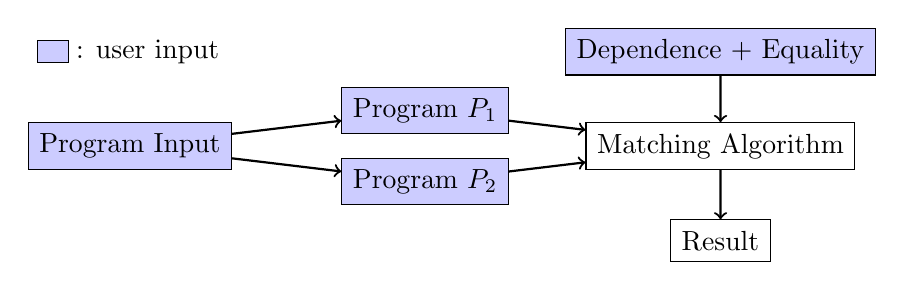
\begin{tikzpicture}[scale=1.5]
\node[Block,Data] (legend) at (-.65, .8) {~};
\node (legendnote) at (.15, .8) {: user input};

\node[Block, Data] (gen) at (0,0) {Program Input};
\node[Block,Data] (p1) at (2.5,0.3) {Program $P_1$};
\node[Block,Data] (p2) at (2.5,-0.3) {Program $P_2$};
\node[Block,Data] (dep) at (5,.8) {Dependence + Equality};
\node[Block] (match) at (5,0) {Matching Algorithm};
\node[Block] (result) at (5,-.8) {Result};

\draw[Block Edge] (gen) -- (p1);
\draw[Block Edge] (gen) -- (p2);
\draw[Block Edge] (p1) -- (match);
\draw[Block Edge] (p2) -- (match);
\draw[Block Edge] (dep) -- (match);
\draw[Block Edge] (match) -- (result);
\end{tikzpicture}

\caption{DiffStream architecture.}
\label{diffstream:fig:system-architecture}
\end{figure}

\section{Writing Specifications in DiffStream}
\label{diffstream:sec:dependence-relation}

In this section we describe how the programmer writes specifications in DiffStream.
Let's look back at the taxi example from before. The second stage of the program
computes the total distance traveled by each taxi by computing the
distance between the current and the previous location, and adding
that to a sum. For this computation to return correct results,
location events for each taxi should arrive in order in its input---a
requirement that must be checked if we want to test the first stage of
the program.

A dependence relation is a symmetric binary relation on events of a
stream with the following semantics.
If $x \dep y$, then the order of
$x$ and $y$ in a stream is significant and reordering them gives us
two streams that are not equivalent. This could be the case if the
consumer of an output stream produces different results depending on
the order of $x$ and $y$.  Thus, the dependence relation can be
thought of as encoding the pairwise ordering requirements of the
downstream consumer.

\begin{figure}[t]
  \centering \footnotesize{}
  \begin{subfigure}[b]{0.46\textwidth}
    \centering
    \begin{lstlisting}[basicstyle=\ttfamily\small]
  (ev1, ev2) ->
      ev1.taxiID == ev2.taxiID
    \end{lstlisting}
    \caption{Specification in DiffStream}
    \label{diffstream:fig:simple-taxi-example-dependency-spec}
  \end{subfigure}%
  \qquad
  \begin{subfigure}[b]{0.46\textwidth}
    \centering
    \KeyDepGraph{tID}
    \caption{Dependence visualized as a graph}
    \label{diffstream:fig:simple-taxi-example-dependency-vis}
  \end{subfigure}%
  \caption[DiffStream example specification 1.]{Example specification in DiffStream for the taxi example. Taxi events with the same \inljava{taxiID} are dependent.}
  \label{diffstream:fig:example-dependencies}
\end{figure}

It is often helpful to visualize dependence relations as unordered
graphs, where nodes are equivalence classes of the dependence
relation. For the taxi example, the dependence relation is visualized
in Figure~\ref{diffstream:fig:simple-taxi-example-dependency-vis}, and it indicates that
events with the same taxi identifier are dependent. In DiffStream,
dependence relations can be specified using a Boolean function on a pair
of events. These functions should be pure and should only depend on
the fields of the two events. The DiffStream specification of the dependence relation from Figure~\ref{diffstream:fig:simple-taxi-example-dependency-vis} is shown in Figure~\ref{diffstream:fig:simple-taxi-example-dependency-spec}.

\begin{figure}[t]
  \centering \footnotesize{}
  \begin{subfigure}[b]{0.56\textwidth}
    \centering
    \begin{lstlisting}[basicstyle=\ttfamily\small,linewidth=7.3cm]
  (ev1, ev2) ->
      ev1.isEOD() ||
      ev2.isEOD() ||
      (ev1.isEOM() && ev2.isEOM()) ||
      (ev1.isTaxiEv() &&
       ev2.isTaxiEv() &&
       ev1.taxiID == ev2.taxiID)
    \end{lstlisting}
    \caption{Specification in DiffStream}
    \label{diffstream:fig:extended-taxi-example-dependency-spec}
  \end{subfigure}%
  \qquad
  \begin{subfigure}[b]{0.36\textwidth}
    \centering
    \ExtendedKeyDepGraph{tID}
    \caption{Dependence visualized as a graph}
    \label{diffstream:fig:extended-taxi-example-dependency-vis}
  \end{subfigure}
  \caption[DiffStream example specification 2.]{Example specification in DiffStream for the extended taxi example. Taxi events with the same \inljava{taxiID} are dependent
      and all events are dependent with end-of-day (EOD) events.}
  \label{diffstream:fig:extended-example-dependencies}
\end{figure}

Now let's consider an extension of the above example where the downstream consumer
computes the total distance traveled by each taxi \emph{per
  day}, and also computes the average daily distance by each taxi
every month. To make this possible, the output of the program under test
is now
extended with special EOD (\emph{end-of-day}) and EOM (\emph{end-of-month})
events. The ordering requirements on this output, while more subtle, can still be
precisely specified using a dependence relation.
For example, EOD events are dependent with taxi events since all events of a specific day have to occur before the EOD event of that day for the total daily distance to be correctly computed. On the other hand, EOM events do not have to be dependent with taxi events since daily distances are computed on EOD events. Therefore, an EOM event can occur anywhere between the last EOD event of the month and the first EOD event of the next month.
The DiffStream specification of the dependence relation and its visualization are both shown in Figure~\ref{diffstream:fig:extended-example-dependencies}.

\begin{figure}[t]
  \centering \footnotesize{}
\begin{tabular}{c}
\begin{lstlisting}[basicstyle=\ttfamily\small,linewidth=9cm]
  (ev1, ev2) -> distance(ev1.loc, ev2.loc) < 1
\end{lstlisting}
\end{tabular}
  \caption[DiffStream example specification 3.]{Example specification in DiffStream where  events are dependent if their locations are close.}
  \label{diffstream:fig:proximity-example-dependencies}
\end{figure}

Several frequently occurring dependence relations can be specified
using a combination of the predicates seen in the above examples. This
includes predicates that check if an event is of a specific type
(e.g. \inljava{isEOD()}, \inljava{isTaxiEv()}), and predicates that
check a field (possibly denoting a key or identifier) of the two
events for equality (e.g. \inljava{ev1.taxiID ==
  ev2.taxiID}). However, it is conceivable that the dependence of two
events is determined based on a complex predicate on their fields.

\begin{figure}[t]
  \centering \footnotesize{}
\begin{tabular}{c}
\begin{lstlisting}[basicstyle=\ttfamily\small,linewidth=10cm]
  (ev1, ev2) -> (ev1.isPunctuation() &&
                 ev2.timestamp < ev1.timestamp) ||
                (ev2.isPunctuation() &&
                 ev1.timestamp < ev2.timestamp)
\end{lstlisting}
\end{tabular}
  \caption[DiffStream example specification 4.]{Example specification in DiffStream where punctuation events, used to enforce progress, depend on other events only if the punctuation timestamp is larger.}
  \label{diffstream:fig:punctuation-example-dependencies}
\end{figure}

Another interesting dependence relation occurs in cases where output streams contain punctuation events.
Punctuations are periodic events that contain a timestamp and indicate
that all events up to that timestamp, i.e., all events \inljava{ev} such that \inljava{ev.timestamp < punc.timestamp}, have \emph{most likely} already occurred.
Punctuation events allow programs to make progress, completing any
computation that was waiting for events with earlier
timestamps. However, since events could be arbitrarily delayed, some
of them could arrive after the punctuation.
Consider as an example a taxi that briefly
disconnects from the network and sends the events produced while disconnected
after it reconnects with the network. These events are usually
processed with a custom out-of-order handler, or are completely
dropped. Therefore, punctuation events are dependent with events
that have an earlier timestamp, since reordering them alters the result of the computation, while they are independent of events with later timestamps. This can be specified in DiffStream as
shown in \Cref{diffstream:fig:punctuation-example-dependencies}.

\section{Differential Testing Algorithm}
\label{diffstream:sec:algorithm}

\Cref{diffstream:alg:equivalence} checks for equivalence of two streams.
As described in the overview, the algorithm has two main features:
(i) it can check for equivalence up to any reordering dictated by a given dependence relation, and
(ii) it is online---it processes elements of the stream one at a time.
In this section we present \Cref{diffstream:alg:equivalence}, our algorithm for checking equivalence of two streams.
We prove that our algorithm is correct, and we show that it is optimal in the amount of state it stores during execution.

\begin{figure}[t]
  \centering
  \normalsize
  \begin{minipage}{0.7\textwidth}
  \begin{algorithmic}[1]
    \Require Equality relation $\equiv$, dependence relation $\dep$
    \Require Connected stream $s$ with $\pi_1(s)=s_1$ and $\pi_2(s)=s_2$
    \renewcommand{\algorithmicrequire}{\textbf{Require:}}
    \Require Relations $\equiv$ and $\dep$ are compatible
    \Function{StreamsEquivalent}{$s$}
    \label{diffstream:line:StreamsEquivalentBegin}
    \State $u_1, u_2 \gets$ empty logically ordered sets
    \State {\color{gray}Ghost state: $p_1, p_2 \gets$ empty logically ordered sets}
    \State {\color{gray}Ghost state: $f \gets$ empty function $p_1\to p_2$}
    \For{$(x, i)$ in $s$}\label{diffstream:line:ProcessElementBegin}
      \State $j \gets 3-i$
      \If{$x$ is minimal in $u_i$ and $\exists y\in \min u_j: x \equiv y$}
      \label{diffstream:line:MatchBegin}
        \State $u_j \gets u_j \setminus \{y\}$
        \State {\color{gray}$p_i \gets p_i \cup \{x\}$};
        {\color{gray}$p_j \gets p_j \cup \{y\}$}\label{diffstream:line:GhostBegin}
        \State {\color{gray}$f \gets f[x\mapsto y]$ \textbf{if} $i=1$
          \textbf{else} $f[y\mapsto x]$}\label{diffstream:line:MatchEnd}
      \ElsIf{$\exists y \in u_j: x \dep y$}\label{diffstream:line:NotEquivalentBegin}
        \State \textbf{return false}\label{diffstream:line:NotEquivalentEnd}
      \Else\label{diffstream:line:UnmatchedBegin}
        \State $u_i \gets u_i \cup \{x\}$\label{diffstream:line:UnmatchedEnd}
      \EndIf\label{diffstream:line:ProcessElementEnd}
    \EndFor
    \State \textbf{return} ($u_1=\emptyset$ and $u_2=\emptyset$)
    \label{diffstream:line:FiniteEquivalent}
    \EndFunction\label{diffstream:line:StreamsEquivalentEnd}
  \end{algorithmic}
  \end{minipage}

\caption{DiffStream algorithm: checking equivalence of two streams.}
% Change \Cref to custom crefname Algorithm
% Note: this doesn't update the LOF or the caption, which still says Figure
\label[algorithm]{diffstream:alg:equivalence}
\end{figure}

\subsection{Background}

Before getting to the algorithm itself, we need to introduce some terminology.
A \emph{stream} $s$ is a bounded or unbounded sequence of elements: $s = \langle
x_1, x_2, \ldots \rangle$.
We write $x \in s$ to denote that $x$ is an element
of $s$, we write $s[n]$ for the $n$th element of $s$, and we write
$s[\mathbin{:} n]$ for the bounded substream of elements up to and including the $n$th
element.

We follow the convention that all elements of a stream (denoted with $x$, $y$, etc.) are distinct. This is so that we can unambiguously refer to the location of $x$ in the stream $s$, and for example, say which of $x$ and $y$ occurs earlier. We use $x \equiv y$ to refer to equality of the \emph{underlying values}, rather than the elements as positioned in the stream.

Two streams $s_1, s_2$ are given as input to the algorithm as
a \emph{connected stream} $s$, which
is a stream obtained by arbitrarily interleaving the elements of $s_1$ and $s_2$.
More
precisely, the elements of the connected stream $s$ are of the form $(x, i)$
such that $i\in\{1, 2\}$ and $x \in s_i$. We can recover the original streams
by using \emph{projections} $\pi_1$ and $\pi_2$: $\pi_1(s)=s_1$ and
$\pi_2(s)=s_2$. Conversely, given a stream $s$, we can form
connected streams using \emph{injections} $\iota_1$ and $\iota_2$: $\iota_1(s)$ is obtained by mapping each $x\in s$ to $(x,1)$, and analogously, $\iota_2(s)$ is obtained by mapping each $x\in s$ to $(x,2)$. Thus, $\iota_1(s)$ and
$\iota_2(s)$ are characterized by
$\pi_1(\iota_1(s))=\pi_2(\iota_2(s))=s$ and
$\pi_1(\iota_2(s))=\pi_2(\iota_1(s))=\emptyset$.
The motivation for connected streams comes from the fact that the streams $s_1$
and $s_2$ are produced by the stream processing system asynchronously.

Next, we need to describe what it means for two streams to be
equivalent.  Our notion of equivalence relies on two
relations on the elements of the streams: an \emph{equality relation},
denoted by $\equiv$, and a \emph{dependence relation}, denoted by
$\dep$. The equality relation is provided by the
user (e.g., in Java by overriding the method $\mathrm{equals()}$) and is required to be an equivalence
relation, that is, it should be reflexive, transitive, and
symmetric. For elements $x$ and $y$, we write $x \equiv y$ instead of
$x = y$ for the equality relation to emphasize that it refers to equality on the underlying values, rather than equality of stream elements.
The dependence relation is required to be symmetric, that is, for elements
$x$ and $y$, $x \dep y$ implies $y \dep x$. Finally, the equality and
the dependence are required to be \emph{compatible}: if $x \dep y$ and
$x \equiv x'$, then $x' \dep y$. The three requirements---the equality
being an equivalence relation, the dependence being a symmetric relation,
and the equality and dependence being compatible---need to be ensured
by the user.

Given a stream $s$, a dependence relation
$\dep$ gives rise to a \emph{logical order} on the elements in $s$:
for elements $x,y\in s$, $x$ logically precedes $y$, denoted by $x<y$,
if $x$ precedes $y$ in the stream and either $x$ and $y$ are dependent or they
are transitively dependent---there are intermediate elements $x_1, \ldots,
x_n\in s$ given in their order of occurrence in $s$ such that
$x\dep x_1 \dep \ldots \dep x_n \dep y$. It can be shown that the logical
order is irreflexive and transitive, that is, it is a strict partial order
on the elements of the stream $s$.
Recall that this makes sense because by convention all the elements are distinct, even though the underlying values may be equivalent according to the equality relation $\equiv$.

\begin{figure}[t]
  \centering
  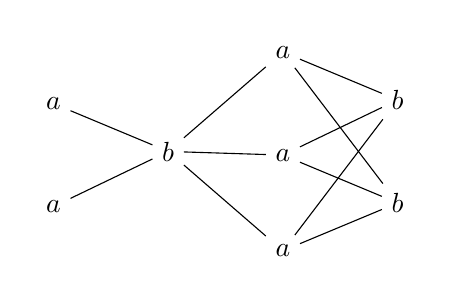
\begin{tikzpicture}
    \matrix (m) [matrix of math nodes, column sep=3em, row sep=0.5em]
    {
              &         & |(a3)|a &         \\
      |(a1)|a &         &         & |(b2)|b \\
              & |(b1)|b & |(a4)|a &         \\
      |(a2)|a &         &         & |(b3)|b \\
              &         & |(a5)|a &         \\
    };
    \path[-]
      (b2) edge (a3) edge (a4) edge (a5)
      (b3) edge (a3) edge (a4) edge (a5)
      (b1) edge (a1) edge (a2) edge (a3) edge (a4) edge (a5);
  \end{tikzpicture}
  \caption[Example logical order of a stream.]{The logical order of the stream from \Cref{diffstream:ex:logical-order}.
  Vertically aligned elements are logically unordered, and for two elements
  that are not aligned, the left one logically precedes
  the right one. The two leftmost elements are minimal.}
  \label{diffstream:fig:logical-order}
\end{figure}

\begin{example}\label{diffstream:ex:logical-order}
  Consider a stream $s=\langle a, a, b, a, a, a, b, b \rangle$.
  The equality relation $\equiv$
  is given by $a\equiv a$ and $b\equiv b$, and the dependence relation
  $\dep$ is given
  by $a \dep b$ (and $b \dep a$). The logical order arising from $\dep$ is shown in
  \Cref{diffstream:fig:logical-order}. The logical orderings between elements
  include $s[1] < s[3]$, $s[3]<s[4]$, and $s[5]<s[7]$. Also $s[4]\parallel
  s[5]$, $s[4]\parallel s[6]$, and $s[5] \parallel s[6]$. Note that
  $s[1] < s[4]$ even though $s[1] \not\dep s[4]$ (both elements are $a$).
  This is because they both depend on $s[3]=b$, which is in between.
\end{example}

Given two streams $s$ and $s'$, an equality relation $\equiv$, and a
dependence relation $\dep$, we say that $s$ and $s'$ are
\emph{equivalent} if they give rise to the same logical order.
More precisely, we say they
are equivalent if there exists a bijective mapping $f\colon s \to s'$,
called a \emph{matching}, that matches equal elements and preserves
the logical order, that is, for every $x,y\in s$, $f(x) \equiv x$ and
$f(x)<f(y)$ if and only if $x<y$. In case the streams are equivalent,
we write $s \equiv_{\dep} s'$, or simply $s \equiv s'$ if the
dependence relation is clear from the context. We call two streams
that are not equivalent \emph{distinguishable}.

If the two streams $s$ and $s'$ are bounded, one way to think about them being
equivalent is as follows: we can get from $s$ to $s'$ in finitely many steps
by either swapping two adjacent logically unordered elements or by replacing
an element with another equal element. In particular, bounded equivalent streams
have the same length.

\begin{example}\label{diffstream:ex:equivalent-streams}
  Streams $s_1=\langle a, c, b\rangle$ and $s_2=\langle c, a, b\rangle$ are
  equivalent with respect to a dependence relation given by $a \dep b$ and
  $c \dep b$. A (unique) matching is given by $f$: $s_1[1]\mapsto s_2[2]$,
  $s_1[2] \mapsto s_2[1]$, and $s_1[3]\mapsto s_2[3]$. Note that the same streams
  are not equivalent with respect to a dependence relation where additionally
  $a \dep c$.
\end{example}

When it comes to unbounded streams, it may be impossible to algorithmically
decide whether they are equivalent or not. For example, consider $s_1=\langle
a, a, a, \ldots \rangle$ and $s_2=\langle b, b, b, \ldots \rangle$ with $a \not\dep b$. Clearly, $s_1\not\equiv s_2$, but an algorithm processing a
connected stream $s$ with $\pi_1(s)=s_1$ and $\pi_2(s)=s_2$
one element at a time
can never reach a conclusion: perhaps eventually $b$'s will start
arriving on the first stream, and $a$'s will start arriving on the second stream.
However, there are situations when an algorithm can reach a definite decision
even if the streams are unbounded. We say that a connected stream $s$ is
\emph{finitely distinguishable} if there is a position $n$ such that for every
continuation $s'$ of $s[\mathbin{:} n]$, the projected streams $\pi_1(s[\mathbin{:} n]
\cdot s')$ and $\pi_2(s[\mathbin{:} n] \cdot s')$ are distinguishable.

\begin{example}
  If $s$ is a connected stream such that $\pi_1(s)=\langle a, a, b\rangle$
  and $\pi_2(s)=\langle a, b\rangle$, and $a \dep b$, then for no continuation
  of $s$ will the two projections ever be equivalent. Thus, $s$ is finitely
  distinguishable.
\end{example}

Given a partial
order $p$, we say that an element $x\in p$ is \emph{minimal} if no other
element is less than $x$. There can be multiple minimal elements in $p$;
we denote the set of minimal elements in $p$ by $\min p$. Given two
partial orders $p$ and $q$ such that $p\subseteq q$, we say that $p$ is
a \emph{prefix} of $q$ if for every element $x\in p$, $p$ also contains all
the elements that are less than $x$ in $q$.

\subsection{Algorithm Description}

We now give a general specification of an online equivalence-checking
algorithm.
The algorithm's inputs are an equality relation
$\equiv$, a dependence
relation $\dep$, and a connected stream $s$ with the projections $s_1=\pi_1(s)$
and $s_2=\pi_2(s)$. We require the equality and
the dependence relations to be compatible. The algorithm provides a
procedure \textsc{StreamsEquivalent} that returns return \textbf{true} or \textbf{false} to report whether or not $s_1 \equiv s_2$. The function
is allowed to iterate over $s$ exactly once.

The algorithm is correct if it has the following behavior:
\begin{enumerate}
  \item[(I)] \textsc{StreamsEquivalent} returns \textbf{true} if and only
    if $s$ is bounded and $s_1,s_2$ are equivalent.
  \item[(II)] \textsc{StreamsEquivalent} returns \textbf{false} if and only
    if either $s$ is finitely distinguishable or it is
    bounded and the streams $s_1,s_2$ are distinguishable.
    Additionally, if $s$ is finitely distinguishable, it returns \textbf{false} after processing $s[n]$ for the first position
    $n$ such that $s[\mathbin{:} n]$ is finitely distinguishable.
\end{enumerate}

\Cref{diffstream:alg:equivalence} achieves the required behavior in the following
way. Intuitively,
it tries to construct a matching to demonstrate equivalence of
$s_1$ and $s_2$. In doing so, as part of its state
it maintains two logically ordered sets
$u_1$ and $u_2$,
both initially empty. Their role is to keep track of the unmatched elements from
$s_1$ and $s_2$, respectively.
In addition to $u_1$ and $u_2$, which constitute the physical state, the
algorithm maintains the so-called ``ghost state,'' written in gray in
\Cref{diffstream:alg:equivalence}. The ghost state need not exist in any real
implementation of the algorithm; its sole purpose is to aid in proving
correctness. As part of the ghost state, the algorithm maintains two additional
logically ordered sets $p_1$ and $p_2$, whose role is to keep track of the
successfully matched prefixes of $s_1$ and $s_2$. In the ghost state, the
algorithm also explicitly
keeps track of the matching $f\colon p_1\to p_2$.

When processing a new element $x$ from $s_i$
(lines \ref{diffstream:line:ProcessElementBegin}--%
\ref{diffstream:line:ProcessElementEnd} in \Cref{diffstream:alg:equivalence}), there are three
distinguished cases:
\begin{enumerate}
  \item The element $x$ is minimal in $u_i$ and there is a corresponding
    unmatched minimal element $y\in u_j$ such that $x \equiv y$ (line
    \ref{diffstream:line:MatchBegin}). In this case
    we remove $y$ from $u_j$. In the ghost state, we add $x$ to $p_i$ and $y$
    to $p_j$, and we extend the matching $f$ to map $x$ to $y$
    or $y$ to $x$, depending on whether $x\in s_1$ or $y\in s_1$ (lines \ref{diffstream:line:GhostBegin}--\ref{diffstream:line:MatchEnd}).
  \item The element $x$ depends on some unmatched element $y\in u_j$ (line
    \ref{diffstream:line:NotEquivalentBegin}).
    If this is the case, then we have detected finite distinguishability
    and the function returns \textbf{false} (line
    \ref{diffstream:line:NotEquivalentEnd}).
  \item If neither of the previous cases holds (line \ref{diffstream:line:UnmatchedBegin}),
    then for every $y\in u_j$, $x$ and $y$ are unequal and independent.
    We add $x$ to $u_i$ as an
    unmatched element (line \ref{diffstream:line:UnmatchedEnd}).
\end{enumerate}

If the whole connected stream has been processed and the function \textsc{StreamsEquivalent} did not return \textbf{false} in line \ref{diffstream:line:NotEquivalentEnd}, it returns \textbf{true} in line \ref{diffstream:line:FiniteEquivalent} if and only if both sets of
unmatched elements are empty.

\begin{example}
    Let us demonstrate the execution of \Cref{diffstream:alg:equivalence} on streams $s_1$ and $s_2$ from
    \Cref{diffstream:ex:equivalent-streams}. Suppose the connected stream given as input
    is
    \[s=\langle (a, 1), (c, 2), (c, 1), (b, 1), (a, 2), (b, 2)\rangle \, .\]
    At the time of processing
    the element $s[3]=(c,1)$, the first two elements have already been processed, and both of them are
    unmatched: $u_1=\{a\}$ and $u_2=\{c\}$. The algorithm detects that the new element $c$ is minimal in
    $u_1$ and it can be matched with the element $c\in u_2$, so it updates the matching $f$ with
    $f(s_1[2])=s_2[1]$ and removes $c$ from $u_2$. Next, it processes $s[4]=(b,1)$: the element $b$
    is not minimal in $u_1$ as it depends on $a\in u_1$. It is also not dependent on any element in $u_2$,
    as $u_2$ is empty. Therefore, it is added to $u_1$, which now contains the ordering $a<b$. Finally,
    the two elements $s[5]=(a,2)$ and $s[6]=(b,2)$ arrive precisely in the right order to be matched with
    the elements in $u_1$, and the algorithm concludes that the streams are equivalent.

    If the dependence relation contained the additional dependence $a\dep c$, the processing would have
    stopped at the element $s[2]=(c,2)$, since the element $c$ from $s_2$ would have been dependent on an
    unmatched element $a\in u_1$. And indeed, the connected stream $s[\mathbin{:} 2]= \langle (a, 1), (c, 2)\rangle$
    would have been finitely distinguishable.
\end{example}

\subsection{Correctness}
\label{diffstream:sec:correctness}

In order to show that the algorithm is correct, we will show that
the loop in \textsc{StreamsEquivalent} (lines \ref{diffstream:line:ProcessElementBegin}--\ref{diffstream:line:ProcessElementEnd}) maintains the following invariants.
\begin{enumerate}
  \item[(I0)] For every $x\in u_1$ and $y\in u_2$, $x$ and $y$
    are unequal and independent:
    $\forall x\in u_1, \forall y\in u_2 : x\not\equiv y \land
    x\not\dep y$.
  \item[(I1)] $p_1$ is a prefix of $s_1$:
    $\forall x\in p_1, \forall y\in s_1 : y < x \Rightarrow y \in p_1$.
  \item[(I2)] $p_2$ is a prefix of $s_2$:
    $\forall x\in p_2, \forall y\in s_2 : y < x \Rightarrow y \in p_2$.
  \item[(I3)] $f\colon p_1\to p_2$ is a maximal matching, that is, it is a matching
    and no extension $f'\colon p_1'\to p_2'$ to proper supersets
    $p_1'\supset p_1$ and $p_2'\supset p_2$ is
    a matching. We also say that $p_1$ and $p_2$ are maximally matched
    prefixes.
\end{enumerate}

\begin{lemma}
  The loop in \textsc{StreamsEquivalent} (lines \ref{diffstream:line:ProcessElementBegin}--\ref{diffstream:line:ProcessElementEnd}) maintains invariants (I0)--(I3).
\end{lemma}

\begin{proof}
  Of the four invariants,
  the one that is least straightforward is (I3), so let us show that it
  holds. In particular, let us show that after the update in lines
  \ref{diffstream:line:GhostBegin}--\ref{diffstream:line:MatchEnd} of \Cref{diffstream:alg:equivalence}, the function $f$
  remains a matching between $p_1$ and $p_2$. Clearly it is still a
  bijection and it maps elements in $p_1$ to equal elements in $p_2$. In
  order to show that it still preserves the logical order, we only need
  to show that for every $x'\in p_1$, $x'<x$ if and only if
  $f(x')<f(x)=y$. Let us show this claim in one direction (the other one
  is analogous).  Assume $x'<x$. By definition, there exists $n\geq 1$
  and elements $x_0, \ldots, x_n\in p_1$ such that $x'=x_0 \dep x_1 \dep
  \ldots \dep x_n=x$.  By the compatibility of $\equiv$ and $\dep$, we
  also have $f(x')=f(x_0) \dep f(x_1) \dep \ldots \dep f(x_n)=y$. By the
  invariant (I2), $y$ does not logically precede $f(x_{n-1})$, so it
  must be $f(x_{n-1})<y$, and finally by transitivity $f(x')<y$. As for
  the maximality of $f$, since (I3) holds at the start of the loop, any extension to $f$ must involve the element $x$ that is
  being processed. Thus, if $f$ can be extended, it is extended by the
  ghost statements in lines \ref{diffstream:line:GhostBegin}--\ref{diffstream:line:MatchEnd}.
\end{proof}

\begin{lemma}\label{diffstream:lem:maximal-prefixes}
  In a bounded connected stream $s$, all maximally matched prefixes
  of $s_1=\pi_1(s)$ and $s_2=\pi_2(s)$ are equivalent.
\end{lemma}

\begin{proof}
  Let $f\colon p_1 \to p_2$ and $g\colon q_1 \to q_2$
  be two maximal matchings, where $p_1$ and $q_1$ are prefixes of $s_1$, and
  $p_2$ and $q_2$ are prefixes of $s_2$. Let $u_1=s_1\setminus p_1,
  u_2=s_2\setminus p_2$, and $v_1=s_1\setminus q_1, v_2=s_2\setminus q_2$
  be the corresponding unmatched elements.
  To show the claim, it suffices to show that $p_1 \equiv q_1$.

  Clearly the identity function $\mathrm{id}\colon p_1\cap q_1
  \to p_1\cap q_1$ is a matching. Let $h\colon p_1'\to q_1'$ be a maximal
  matching between $p_1$ and $q_1$ that extends $\mathrm{id}$; thus, $p_1'$ and
  $q_1'$ are prefixes such that $p_1\cap q_1 \subseteq p_1' \subseteq p_1$
  and $p_1\cap q_1 \subseteq q_1' \subseteq q_1$. To show
  $p_1 \equiv q_1$, it suffices to show that $p_1'=p_1$ and $q_1'=q_1$.

  First we note that for the matchings $f,g,h$, an analog of the invariant (I0)
  holds. In particular, the sets $p_1\setminus p_1'$ and $q_1\setminus q_1'$,
  as well as $v_1$ and $v_2$ are pairwise independent
  and unequal. Moreover, let us set $p_2'=f(p_1')$ and $q_2'=g(q_1')$.
  The sets $p_2\setminus p_2'$ and $q_2\setminus q_2'$ are also pairwise
  independent and unequal. Let us show the claim for $p_1\setminus p_1'$ and $q_1\setminus q_1'$. Suppose first that $x\in p_1\setminus p_1'$ and $y\in q_1\setminus
  q_1'$ are elements such that $x\dep y$. Since $x$ and $y$ are both in
  $s_1$, we either have $x<y$ or $y<x$. If $x<y$, then
  we have $x\in q_1$ since $q_1$ is a prefix, and consequently $x\in p_1\cap q_1\subseteq
  p_1'$, which is a contradiction. Likewise, $y<x$ leads to $y\in q_1'$, which is also a contradiction. Suppose now that $x\in p_1\setminus p_1'$ and $y\in q_1\setminus
  q_1'$ are elements such that $x\equiv y$.
  They cannot both be minimal,
  for we would be able to extend $h$ with
  $h(x)=y$. Thus, one of $x$ and $y$ has a logical predecessor; say $x'\in p_1\setminus p_1'$ is such that $x'<x$. Without loss of generality, $x' \dep x$. Since
  $\equiv$ and $\dep$ are compatible, this leads to $x' \dep y$, which we
  have just shown to be impossible.

  We are now ready to prove $p_1'=p_1$ ($q_1'=q_1$ is analogous).
  For the sake of contradiction, suppose that $p_1'\neq p_1$, that is,
  there exists an element $x\in p_1\setminus p_1'$. Note that $x\notin
  q_1$, that is, $x\in v_1$.  We send $x$ to $s_2$ via $f$; we have
  $f(x)\in p_2\setminus p_2'$. The element $f(x)$ cannot be in $v_2$
  since $x\in v_1$ and $x\equiv f(x)$. The element $f(x)$ also cannot
  be in $q_2\setminus q_2'$, since it is in $p_2\setminus p_2'$ and
  $f(x)\equiv f(x)$. Hence, $f(x)\in q_2'$.  Now we pull $f(x)$ back
  to $s_1$ via $g$ and $h$. Set $x_1=h^{-1}(g^{-1}(f(x)))$; we have
  $x_1 \in p_1'$. Since $x\notin p_1'$, $x_1$ and $x$ are distinct
  elements such that $x_1\equiv x$. We can continue iterating the
  described process. Suppose we have defined distinct elements $x_1,
  \ldots, x_n\in p_1'$ for some $n\geq 1$ such that $x\equiv x_1\equiv
  \ldots \equiv x_n$. We send $x_n$ to $s_2$ via $f$ and note that
  neither $f(x_n)\notin v_2$ (otherwise we would have $x\in v_1$,
  $f(x_n)\in v_2$, and $x\equiv f(x_n)$) nor $f(x_n)\in q_2\setminus
  q_2'$ (otherwise we would have $f(x)\in p_2\setminus p_2'$,
  $f(x_n)\in q_2\setminus q_2'$, and $f(x)\equiv f(x_n)$). Therefore,
  $f(x_n)\in q_2'$ and we can bring it back to $s_1$ via $g$ and $h$
  to get a well-defined element $x_{n+1}= h^{-1}(g^{-1}(f(x_n)))\in
  p_1'$. Suppose $x_{n+1}=x_{k}$ for some $k$ with $1\leq k \leq
  n$. By removing $k$ layers of application of $h^{-1}\circ
  g^{-1}\circ f$, we conclude that $x_{n+1-k}=x$, which cannot be
  since $x_{n+1-k}\in p_1'$ and $x\notin p_1'$. Therefore, $x_{n+1}$
  is distinct from all previously defined elements.

  By defining the described process, we have shown that
  there are infinitely many distinct elements in $p_1'$, which cannot be
  since $p_1'$ is a finite set. Hence, $x\in
  p_1\setminus p_1'$ cannot exist in the first place, and we have
  established that $p_1=p_1'$. Analogously,
  we have $q_1=q_1'$, and since $p_1'\equiv q_1'$, we also have $p_1\equiv q_1$.
  Finally,
  using $p_1\equiv q_1$ as a link, we establish that $p_2\equiv p_1\equiv
   q_1\equiv q_2$, that is, all the maximally matched prefixes in $s$ are
  equivalent.
\end{proof}

\begin{lemma}\label{diffstream:lem:finitely-distinguishable}
  If \textsc{StreamsEquivalent} returns \textbf{false} in line \ref{diffstream:line:NotEquivalentEnd} while processing $s[n]$ for
  some $n\geq 1$, then the connected stream $s[\mathbin{:} n]$ is finitely distinguishable.
\end{lemma}

\begin{proof}
  Let $s[n]=(x,1)$ and assume that \textsc{ProcessElement} returns
  \textbf{false} in line \ref{diffstream:line:NotEquivalentEnd} when processing $s[n]$.
  Since the condition in line \ref{diffstream:line:NotEquivalentBegin} was satisfied,
  there exists $y\in u_2$ such that $x\dep y$.
  Without loss of generality, let $y$ be a minimal such element in $u_2$.

  The challenge here is that even though $f$ can never be extended to match
  either $x$ or $y$, it is plausible that $s[\mathbin{:} n]$ can nevertheless be
  extended to $s'$ with a completely different matching that somehow accommodates both elements.
  To show that such a scenario is impossible, suppose
  $s'$ is an extension of $s[\mathbin{:} n]$ such that $\pi_1(s')=s_1'\supseteq s_1$, $\pi_2(s')=s_2'\supseteq s_2$, and suppose
  $g\colon s_2'\to s_1'$ is a matching (it helps to view $g$ in the direction opposite of $f$). Since $x \dep y$ and $g(y)\equiv y$, we have $x \dep g(y)$,
  so $x$ and $g(y)$ are logically ordered in $s_1'$. There are three possibilities:
  $g(y)=x$ (the elements are identical),
  $g(y)<x$, or $x<g(y)$.

  The first possibility can easily be discarded. From $g(y)=x$ it follows
  that $x\equiv y$. The elements $x$ and $y$ cannot both be minimal elements unmatched by $f$, otherwise $x$ would have been matched in lines
  \ref{diffstream:line:MatchBegin}--\ref{diffstream:line:MatchEnd}. Therefore, either there is
  $x'\in u_1$ such that $x'<x$ and $x'\dep x$, or there is $y'\in u_2$ such that
  $y'<y$ and $y'\dep y$. In the former case we have $x' \dep y$,
  contradicting the invariant (I0), and in the latter case we have
  $x \dep y'$ and $y'<y$, contradicting the choice of $y$ as a minimal
  unmatched element such that $x\dep y$.

  The second possibility, that $g(y)<x$, can be discarded as follows. Set $y_0=y$.
  The element $g(y_0)$
  cannot be in $u_1$ as that would break the invariant (I0); therefore it
  has to be in $p_1$. We can send it to $p_2$ via $f$; let
  $y_1=f(g(y_0))$.
  Since $y_0\notin p_2$, $y_0$ and $y_1$ are distinct elements such that
  $y_0\equiv y_1$.
  We iterate the process: suppose we have defined the elements $y_1, \ldots, y_n
  \in p_2$ for some $n\geq 1$ such that all of them are equal to $y_0$, and all of
  them together with $y_0$ are distinct.
  Since $g(y_n) \dep x$, $g(y_n)$ and $x$ are logically ordered. It cannot be
  $g(y_n)\geq x$, as
  that would imply $g(y_n) > g(y_0)$ and consequently $y_n>y_0$. But then,
  since
  $y_n\in p_2$ and $p_2$ is a prefix, we would have $y_0\in p_2$, which
  is a contradiction. Thus, $g(y_n)<x$ and consequently $g(y_n)\in p_1$ due to the
  invariant (I0). Hence, $y_{n+1}=f(g(y_n))$ is a well-defined element such
  that $y_{n+1}\in p_2$. Clearly $y_{n+1}$ is distinct from $y_0$, and
  $y_{n+1}\equiv y_0$. Suppose $y_{n+1}=y_{k}$ for some $k$ with $1\leq k \leq n$.
  By ``pealing off'' $k$ layers of applications of $f$ and $g$, we would
  get $y_{n+1-k}=y_0$, which is a contradiction. Therefore, the new element is
  distinct from every previously defined element. We have thus defined infinitely
  many distinct elements in the finite set $p_2$, which is a contradiction.
  Hence, $g(y) \nless x$.

  The third possibility, that $x<g(y)$, is discarded by a similar argument.
  The idea is again to start from $x_0=x$ and define an infinite sequence of
  distinct elements $x_1, x_2, \ldots$ in $p_1$, all of which are equal to and
  distinct from $x_0$. However, the argument that shows the
  sequence is well-defined is slightly different. Similarly as before,
  given $x_n$ for $n\geq 1$ we start by arguing that $g^{-1}(x_n)\in p_2$.
  We first establish that $g^{-1}(x_n)<y$, as otherwise
  $g^{-1}(x_n)\geq y > g^{-1}(x_0)$
  would imply $x_n > x_0$ and consequently $x_0\in p_1$. Next, if $g^{-1}(x_n)\in
  u_2$, then we argue as in the first possibility: either $x$ and $g^{-1}(x_n)$
  can be matched, or there is $x'<x$ in $u_1$ such that $x'\dep g^{-1}(x_n)$, contradicting the invariant (I0), or there is $y'<g^{-1}(x_n)<y$ in $u_2$ such
  that $x \dep y'$, contradicting the minimality of $y$. Hence, $g^{-1}(x_n)\in p_2$
  and $x_{n+1}=f^{-1}(g^{-1}(x_n))$ is well-defined. Showing that it is distinct from previously
  defined elements is done using the same argument as before. Thus, we again
  reach a contradiction, and $x \nless g(y)$.

  By discarding all three possibilities, we conclude that the extension of
  $s[\mathbin{:} n]$ to a connected stream $s'$ such that $s_1'\equiv s_2'$
  does not exist. Hence, $s[\mathbin{:} n]$ is finitely distinguishable.
\end{proof}

\begin{theorem}
  \label{diffstream:thm:correctness}
  \Cref{diffstream:alg:equivalence} is correct.
\end{theorem}

\begin{proof}
  We first show that \Cref{diffstream:alg:equivalence} satisfies the correctness
  condition (I). If
  \textsc{StreamsEquivalent} returns \textbf{true} in line \ref{diffstream:line:StreamsEquivalentEnd}, then
  the whole connected stream $s$ has been processed. Hence, $s$ is bounded.
  Moreover, in this case both $u_1$ and $u_2$
  are empty, implying $p_1=s_1$ and $p_2=s_2$. Therefore, $s_1\equiv s_2$ follows from the invariant (I3).
  Conversely, if $s$ is bounded and $s_1,s_2$ are equivalent, by
  \Cref{diffstream:lem:finitely-distinguishable},
  \textsc{StreamsEquivalent} does not
  return \textbf{false} on line \ref{diffstream:line:NotEquivalentEnd}, and the loop in lines
  \ref{diffstream:line:ProcessElementBegin}--\ref{diffstream:line:ProcessElementEnd} finishes. By the invariant (I3) and \Cref{diffstream:lem:maximal-prefixes}, $f$ must fully
  match $s_1$ and $s_2$. Hence, $u_1$ and $u_2$ are empty and
  \textsc{StreamsEquivalent} returns \textbf{true}.

  Next, we show the correctness condition (II).
  If \textsc{StreamsEquivalent} returns \textbf{false}, it either returns \textbf{false} in line \ref{diffstream:line:NotEquivalentEnd} and $s$ is finitely
  distinguishable by \Cref{diffstream:lem:finitely-distinguishable}, or it returns \textbf{false} in line \ref{diffstream:line:StreamsEquivalentEnd}. In the latter case, $s$ is bounded and one of $u_1$ and $u_2$ is not empty. Hence, $s_1$ and $s_2$ are distinguishable by the invariant (I3) and \Cref{diffstream:lem:maximal-prefixes}.
  Conversely, if $s$ is bounded and $s_1,s_2$ are distinguishable, by (I)
  the function \textsc{StreamsEquivalent} does not return \textbf{true},
  so it returns \textbf{false}.

  It remains
  to show that if $s$ is finitely distinguishable, then \textsc{StreamsEquivalent} returns \textbf{false} in line \ref{diffstream:line:NotEquivalentEnd} for the
  first position $n$ such that $s[\mathbin{:} n]$ is finitely distinguishable. Clearly \textsc{StreamsEquivalent} does not return \textbf{false} on line \ref{diffstream:line:NotEquivalentEnd} when processing $s[k]$
  for $k<n$, since in that case by \Cref{diffstream:lem:finitely-distinguishable} already $s[\mathbin{:} k]$ would be finitely distinguishable. Let $s[n]=(x,1)$ and let $u_1$ and $u_2$ be the logically ordered sets of unmatched elements at the start of
  the loop when processing $s[n]$.
  If $x$ can be matched with an element $y\in \min u_2$, then we
  extend $s[\mathbin{:} n]$ with $\iota_1(u_2\setminus\{y\})$
  followed by $\iota_2(u_1)$, with the elements of $u_i, i\in\{1,2\}$
  given in the order in
  which they appear in $s[\mathbin{:} {n-1}]$.
  Likewise, if $x\not\dep y$ for every $y\in u_2$, then we extend $s[\mathbin{:} n]$
  with
  $\iota_1(u_2)$ followed by $\iota_2(u_1\cup\{x\})$. In either case, from
  the invariants
  (I0)--(I3) it follows that \Cref{diffstream:alg:equivalence} would decide that the
  two streams in the
  extension are equivalent, and since the algorithm is correct
  for bounded equivalent streams, the streams would indeed be equivalent.
  Therefore, in both cases the connected stream $s[\mathbin{:} n]$ would not be
  finitely distinguishable. Since $s[\mathbin{:} n]$ is finitely distinguishable,
  the only remaining option is that there exists $y\in u_2$ such that $x\dep y$, and hence \textsc{StreamsEquivalent} returns \textbf{false} in line \ref{diffstream:line:NotEquivalentEnd} when processing $s[n]$.
\end{proof}

\subsection{Optimality}
\label{diffstream:sec:optimality}

When it comes to stateful stream processing programs, space usage is an
important topic. If a stateful stream processing program inadvertently stores
too much of the stream's history, since the stream is potentially unbounded,
the program's space usage may grow unboundedly as well. In case of
\Cref{diffstream:alg:equivalence}, its space usage may indeed grow unboundedly. Since
\Cref{diffstream:alg:equivalence} stores sets of unmatched elements, it can be forced to
keep the complete history of the connected stream it takes as input. For example,
this would happen on a connected stream $s$ such that $\pi_1(s)=\langle a, a,
\ldots\rangle$, $\pi_2(s)=\langle b, b, \ldots\rangle$, with $a\not\equiv b$ and $a\not\dep b$.
However, it turns out that for a correct equivalence-matching algorithm there
is no way around this: a correct
equivalence-checking algorithm must store a certain amount
of unmatched elements in one way or another. In each step,
\Cref{diffstream:alg:equivalence} stores
minimal sets of unmatched elements (the complements of maximally matched
prefixes), and as we show in this subsection, in this sense it is optimal.


Recall that by \Cref{diffstream:lem:maximal-prefixes}, in a bounded connected stream $s$ with $s_1=\pi_1(s)$ and $s_2=\pi_2(s)$, all maximally matched prefixes of $s_1$
and $s_2$ are equivalent. It follows that their complements---minimal sets
of unmatched elements---are equivalent as well. More precisely, let $(p_1,p_2)$
and $(q_1,q_2)$ be two pairs of maximally matched prefixes such that
$p_i,q_i\subseteq s_i$ for $i\in\{1,2\}$, and let $u_i=s_i\setminus p_i$
and $v_i=s_i\setminus q_i$ for $i\in\{1,2\}$. Then $u_1\equiv v_1$ and
$u_2\equiv v_2$. This allows us to define up to equivalence a function
$u(s)=(u_1,u_2)$, where $u_1$ and $u_2$ are any minimal sets of unmatched elements in $s_1$ and $s_2$. We write $(u_1,u_2)\equiv (v_1,v_2)$ to mean
$u_1\equiv v_1$ and
$u_2\equiv v_2$.

If a bounded connected stream $s$ with $u(s)=(u_1,u_2)$ is not finitely
distinguishable, then an analog of the invariant (I0) holds for $u_1$ and $u_2$:
for every $x\in u_1$ and $y\in u_2$, $x\not\equiv y$ and $x\not\dep y$.

\begin{theorem}\label{diffstream:thm:optimality}
  \Cref{diffstream:alg:equivalence} is optimal. More precisely,
  let $A$ be any other \emph{correct} algorithm for the equivalence-checking problem.
  If $s$ and $s'$ are two bounded connected streams that are not finitely distinguishable,
  and if \Cref{diffstream:alg:equivalence} reaches a different state after processing $s$ and $s'$, then $A$ reaches a different state after processing $s$ and $s'$.
\end{theorem}

\begin{proof}
  The state stored by \Cref{diffstream:alg:equivalence} on processing a string $s$ is $u(s)$.
  Suppose a correct equivalence-checking algorithm reaches the same state
  after processing $s$ and $s'$. Let $u(s)=(u_1,u_2)$ and $u(s')=(u_1',u_2')$.
  We extend both $s$ and $s'$ with $\iota_1(u_2)$ followed by $\iota_2(u_1)$.
  It is not difficult to see that the
  two connected streams in the extension of $s$
  are equivalent, and the streams in the extension of $s'$ are not equivalent.
  However, since the algorithm is deterministic, it would come to the same
  decision for both extensions, which contradicts its correctness.
\end{proof}

\section{Practical Bounds on Space Usage}
\label{diffstream:sec:practical-bounds}

While the space used by \Cref{diffstream:alg:equivalence}  can grow with the input stream in the worst case, \Cref{diffstream:thm:optimality} shows that it is impossible to write an algorithm which uses a smaller amount of space. In addition to this result, it is possible to give concrete bounds on the space usage in certain cases. Here we discuss some patterns that we have encountered, including the examples we implemented in \Cref{diffstream:sec:evaluation}, and how bounds on the space usage can be derived for these patterns.

The simplest pattern is differential testing of sequential outputs: both streams are completely ordered, i.e., any two events are dependent. In this case, any differential testing algorithm must at least keep track of the difference of the two streams seen so far (assuming their prefixes are equal). For example, suppose both streams are sequences of integers, and one stream has seen $m$ integers and the other has seen $n$ integers, where $m < n$. Then if the first $m$ integers are equal, any matching algorithm must keep track of the remaining $(n - m)$ integers. Thus, the space usage of the algorithm is bounded by the maximum \emph{drift} between the two streams, defined as the difference in the number of events produced.
In practice, such drift is typically bounded since inputs arrive at the same rate for both the implementations, and
most systems try to ensure that no operator in the stream processing dataflow graph lags behind the others by accumulating a large queue of unprocessed inputs.
This dependence relation pattern (and the resulting bound) occurs in the case studies of \Cref{diffstream:ssec:evaluation-wordcount,diffstream:ssec:evaluation-mapreduce}.

A second common pattern is \emph{key-based parallelism}, where events with the same key are dependent, but events with different keys are independent. In such a case, considering the drift between the two streams is not enough. For example, suppose there are only two keys, $a$ and $b$, and one stream produces $n$ $a$s, but the other stream produces $n$ $b$s. Then although the two streams are producing the same number of items, because stream 1 never produces an $a$ and stream 2 never produces a $b$, any algorithm for correct matching must keep at least the $a$s and the $b$s so far until they are matched on the other stream. To address this, we can obtain a bound on the space by considering the drift \emph{per key}. In general, ``keys'' can be generalized as dependent subsets of events, and a bound can be obtained by taking the maximum drift on any dependent subset, together with the number of independent keys in the input. This dependence relation pattern (and the resulting bound) occur in the case study of \Cref{diffstream:ssec:evaluation-keyby}.
Related to key-based parallelism, \emph{fully independent parallelism} (where all input events are independent) occurs in the case studies of \Cref{diffstream:ssec:evaluation-mapreduce,diffstream:ssec:evaluation-onlinemonitoring}.

Finally, we have encountered cases where the input includes special synchronization events, such as punctuation marks and end-of-day markers, as described in \Cref{diffstream:sec:dependence-relation}. These events are dependent on all other events. If both input programs to the differential testing algorithm produce these events at regular intervals, then the space usage becomes bounded. In particular, suppose that the \emph{frequency} of such events is at least one in every $k$ events, and the \emph{drift} restricted only to such events is $d$. Then the space usage of our algorithm is at most $k \times d$.

To ensure that bounded drift holds between the two streams in practice, one approach would be to leverage \emph{back-pressure} of the underlying system~\cite{collins2009flexible,kulkarni2015twitter-heron,chen2017governor}.
In particular, back-pressure may prevent drift from growing in cases where one implementation is significantly faster than the other, since the system would slow down the fast implementation to prevent unbounded buffering.

\section{Evaluation}
\label{diffstream:sec:evaluation}

We implemented the matcher algorithm in DiffStream, a differential
testing library written in Java. The matcher can be used to test
programs in any distributed stream processing system given an output
interface. For our case studies we chose Flink as the target platform
because it is one of the most widely used distributed stream
processing
frameworks~\cite{stackoverflow-flink}. We
integrated DiffStream with JUnit-QuickCheck~\cite{junit-quickcheck} to
support generation of streams of random input values.

Our first case study (\Cref{diffstream:ssec:evaluation-keyby}) is used to qualitatively measure the developer effort needed to test an application with non-trivial ordering dependency in its output. In the second case study (\Cref{diffstream:ssec:evaluation-wordcount}) we demonstrate that getting performance benefits from parallelization in Flink might require an elaborate implementation and we illustrate how our tool can be used to streamline that process. In the third case study (\Cref{diffstream:ssec:evaluation-mapreduce}), we show that our framework is successful in finding real bugs while largely avoiding false positives by adapting a set of non-deterministic MapReduce programs from the literature~\cite{xiao2014nondeterminism}. The final case study (\Cref{diffstream:ssec:evaluation-onlinemonitoring}) investigates the performance overhead when using DiffStream{} for online monitoring of long-running applications.

\subsection{Taxi Distance}
\label{diffstream:ssec:evaluation-keyby}

This case study illustrates the process that one has to follow in
order to test their implementation using our tool. Recall the taxi
distance example in \Cref{diffstream:ssec:motivating-examples}. This example
shows two seemingly equivalent implementations of the same query that
produce different results in the presence of parallelism.  Here is an
instantiation of that example in Flink; the first implementation
preserves the order of events for each key, while the second one does
not:

\medskip

\begin{lstlisting}[basicstyle=\ttfamily\small,frame=none]
  inStream.keyBy("taxiID").project("taxiID", "position");
\end{lstlisting}
\begin{lstlisting}[basicstyle=\ttfamily\small,frame=none]
  inStream.project("taxiID", "position").keyBy("taxiID");
\end{lstlisting}

\medskip

Note that both implementations preserve the order when executed
sequentially. Since such subtle differences are difficult to spot
manually, we would like to be able to test a parallel implementation
against a sequential one, before deploying it. A slightly simplified
example of a test that can exercise this bug using our framework is
shown in \Cref{diffstream:fig:keybytest}.
\begin{figure}[tb]
    \centering
\begin{tabular}{c}
\begin{lstlisting}[linewidth=12cm,basicstyle=\ttfamily\normalsize]
public void testKeyBy() throws Exception {
    StreamExecutionEnvironment env = ...;

    DataStream input = generateInput(env);

    StreamEquivalenceMatcher matcher =
        StreamEquivalenceMatcher.createMatcher(
            sequentialImpl(input), parallelImpl(input),
            (ev1, ev2) -> ev1.taxiID == ev2.taxiID);

    env.execute();
    matcher.assertStreamsAreEquivalent();
}
\end{lstlisting}
\end{tabular}
    \caption{DiffStream example code.}
    \label{diffstream:fig:keybytest}
\end{figure}{}
%
First, the Flink execution environment is initialized and the dataflow
graph is setup. Then, a random input stream is generated and fed to
both implementations, that are finally compared using the matcher for
output equivalence.

Notice that the final argument of the matcher is a lambda expression
representing the dependence relation that is expected from the
consumer of the output. This specific instantiation represents the
dependence that was shown in \Cref{diffstream:fig:simple-taxi-example-dependency-spec}---i.e., that two items are dependent (and thus must be ordered) if
they have the same \inljava{taxiID}. If the user did not want to test
differences in the ordering of the output, they can use
\inljava{(ev1, ev2) -> false} as the dependence relation.


In order to compare the effort required to write a test with and
without using our framework, we manually implemented a test that
exercises this bug. The manually implemented matcher spans two Java
classes, totaling around 100~LoC (in contrast to the 13~LoC of the
test in our framework shown in \Cref{diffstream:fig:keybytest}). This does not
include input generation, for which we used JUnit QuickCheck. The
manually implemented matcher keeps two hashmaps---one for each
implementation---that map keys to lists, in order to encode the
dependence of events of the same key. It appends each output item to
the list associated with its key. After the two implementations stop
executing, it checks that the two hashmaps represent equivalent
output. Note that this manual matcher is not online, in the sense that
the two implementations have to stop producing outputs for it to make
a decision. We also implemented an online version of it by extending
it with 30 more lines of code.

The important point is that the dependence relation abstraction
enables the design of a reusable testing framework that can be used
for testing applications with different ordering requirements on their
outputs. In contrast, the main drawback of the manual matcher is that
it is tied to a specific ordering requirement on the output; whenever
a user wants to write a test that requires a different output
dependence relation, they would have to implement a new matcher that
maintains the output in a data structure suitable for the specific
dependence. This can quickly become an overhead if the user wants to
write tens or hundreds of tests for different parts of their
application.

In summary, we have shown that using our tool to write a test for a stream processing application is significantly easier than writing custom tests ($\sim$10 LoC vs.~$\sim$100 LoC). In addition, our tool offers additional flexibility, as it can be used to test any two implementations just by changing the dependence relation given to it. This flexibility reduces the effort needed to implement tests for an application. It also exposes ordering requirements, forcing the developer to think about them explicitly.

\subsection{Topic Count}
\label{diffstream:ssec:evaluation-wordcount}

The main goal of our second case study is to show that achieving parallelism in distributed stream processing programs can be very difficult and require a drastically more complicated solution than the sequential code.
In particular, we consider the example introduced
in \Cref{diffstream:ssec:motivating-examples}, that involves counting topics associated with words in a long document
and outputting the most frequent topic as the overall topic of the document.
The documents are streamed word by word, with end-of-file markers
delineating words in different documents.
In the sequential solution (\Cref{diffstream:ex:overview-complex}, top), we process each word by querying the topic for that word, then updating the total count for that topic; when we get end-of-file, we emit the counts. We feed this output to a second operator \emph{count max}, which finds the maximum over all topics of the count.

At first, one may think that going from a sequential to a parallel program is
simply a matter of setting the Flink's parallelism parameter to more than 1.
Unfortunately, this is not the case. Consider the first operator in the
sequential dataflow shown in \Cref{diffstream:ex:overview-complex} (top). The problem with
parallelizing this operator is that an end-of-file marker for a particular
document would only be processed by a single sub-operator; thus the other
sub-operators would not be able to properly delineate words from this document
and the next one. Another way of stating the problem is to say that even
though the words themselves are independent, they are dependent on the
end-of-file markers, and thus the obvious parallelization is not possible.
A differential test that compares the sequential dataflow
to the same dataflow with parallelism set to more than 1
quickly discovers that the two versions are indeed not equivalent.

Instead, a correct parallel solution (\Cref{diffstream:ex:overview-complex}, bottom) works as follows. We first attach logical timestamps to each word in the input, corresponding to the number of the document that we are currently processing.
We then replace end-of-file markers,
which act as explicit punctuation in the stream, with punctuated watermarks---%
a mechanism in Flink that
informs the dataflow operators about the
passage of logical time. Unlike the explicit end-of-file markers that cannot
be shared by multiple sub-operators, the watermarks are seamlessly propagated
by the system. In effect, they allow us to break the explicit dependence
between words and end-of-file markers in the input stream, allowing the
later stages of the dataflow to be parallelized. We parallelize with \emph{key-by} (keys can be assigned arbitrarily to words), and query the database for each word. The next operator is a tumbling window which uses the logical timestamps from earlier to form the window of events \emph{for a single document}, still parallelized. Finally, we sum up the values in each window by topic, and in the last stage \emph{count max} we find the maximum over all topics of the count.

In our search for a correct parallel solution, we consulted with Flink users
on the Flink mailing list. Several iterations of feedback were needed to find a correct parallel implementation, and this shows that it is not obvious. Having the differential testing framework helped guide the search by quickly dismissing wrong implementations. The final solution is the
dataflow shown in \Cref{diffstream:ex:overview-complex} (bottom), consisting of 6
dataflow operators and twice as many lines of code as the sequential solution.

\begin{figure}[t]
  \centering
    \begin{tabular}{p{2.8cm} | p{2.5cm} | p{1.4cm}p{1.4cm}p{1.4cm}p{1.4cm}}
    & & \multicolumn{4}{c}{{Speedup due to parallelism (par.)}} \\
    Solution & Lines of Code & par. 2 & par. 4 & par. 6 & par. 8 \\
    \hline
    Sequential & 68 & -- & -- & -- & -- \\
    Correct Parallel & 133 & 2.01 & 4.33 & 5.0 & 4.99 \\
    \end{tabular}

  \bigskip

\caption[Manual parallelism case study results.]{Results of the second case study on difficulty of writing parallel code.}
\label{diffstream:fig:word-count-evaluation}
\end{figure}

It is not necessarily true that a solution that seems parallel achieves a speed-up in practice.
We therefore finally need to measure the performance of the parallel solution to show that it indeed takes advantage of parallelism and scales performance with the level of parallelism.
We evaluated our parallel solution on an input stream of 5 documents, each consisting of
500,000 words randomly selected from a list of 10,000 most common English words.
Each word had previously been randomly assigned one of 20 topics, and the
association had been stored in a standalone Redis key-value store. The purpose
of having the Flink program query the Redis store was to simulate a series of
non-trivial operations that would benefit by being parallelized.
We executed this experiment on a server with an Intel Xeon Gold 6154 processor and 384 GB of memory.
The results
of the evaluation are shown in \Cref{diffstream:fig:word-count-evaluation}. By increasing
parallelism from 1 to 6, the execution time decreases from 80 s to
16 s (on our setup, the benefits taper off after 6).

In summary, although there is a clear performance benefit in having a parallel solution (\Cref{diffstream:fig:word-count-evaluation}), the correct solution is difficult to find, as evidenced qualitatively by our search and discussions on the Flink mailing list, and quantitatively because it has about twice as many lines of code as the sequential solution.
Applying differential testing to the parallel solution ensures that bugs were not introduced in the process.

\subsection{Real-World MapReduce Programs}
\label{diffstream:ssec:evaluation-mapreduce}

To determine whether our testing framework can successfully find bugs in real-world programs, we surveyed the literature for empirical studies which have collected and categorized bugs in stream-~and batch-processing programs. We excluded works that focus on job failures and performance issues~\cite{schroeder2009large,kavulya2010analysis,li2013characteristic,zhou2015empirical}, as they do not provide examples of semantic bugs where the output might be incorrect.
In contrast, Xiao et. al.~\cite{xiao2014nondeterminism} study
nondeterminism due to parallelism
in MapReduce jobs in production workflows,
identifying both real bugs as well as several nondeterministic code patterns which are bug-free.
This empirical study provides a good starting point to evaluate whether our framework can successfully identify the bugs, while not falsely flagging the bug-free examples.

By examining 507 custom (i.e., user-written) reduce functions, the study identifies 5 common reducer patterns (spanning 258 of the custom reducers) which are \emph{non-commutative} on general input data, meaning that there is potential for nondeterminism in the output due to parallelism.
An example reducer pattern reported by the study is shown in \Cref{diffstream:fig:mapreduce-case-study-code}~(left).
While the original custom reducers are not publicly available, the 5 code patterns are nevertheless minimal test cases which exhibit the same behavior, and a large majority of non-commutative reducers (88\%) were found to fall into these categories.
However, as the study notes, there are two reasons why code written using these patterns might not be erroneous. First, with certain input assumptions, the nondeterminism may disappear (this is possible in 4 out of 5 patterns). Second, nondeterminism may simply be acceptable for the particular application (this is most conceivable in 3 out of 5 patterns).
We therefore evaluate our testing framework for each of the five patterns, considering three possibilities for the application-specific requirements: determinism (nondeterminism is not acceptable), determinism under certain
input assumptions, and no determinism required. We want to answer the following questions, corresponding to these three possibilities:
\begin{enumerate}
\item[Q1.] If determinism is required on all inputs, can we write a test which successfully detects the nondeterminism and reports a bug?
\item[Q2.] If determinism is required but only under certain input assumptions, can we write a test using those input assumptions to avoid a false positive?
\item[Q3.] If determinism is not required at all, can we write a test which avoids a false positive?
\end{enumerate}
For each question, we implement the reducer adapted to the streaming setting, and run DiffStream to compare a sequential and parallel version.
The results are summarized in \Cref{diffstream:fig:mapreduce-case-study-summary}, where columns 1, 2, and 3 correspond to the above three questions, respectively.

\begin{figure}[tb]
    \centering \small

    \setlength\tabcolsep{1em}
    \begin{tabular}{c|ccc}
          & \multicolumn{3}{c}{\underline{Application-Specific Requirements}} \\
         Code pattern & Determinism & \makecell{Determinism under \\ input assumptions} & \makecell{None \\ (nondeterminism acceptable)} \\
         \hline
         \texttt{SingleItem} & \cmark{} & \cmark{} & \namark{} \\
         \texttt{IndexValuePair} & \cmark{} & \cmark{} & \namark{} \\
         \texttt{MaxRow} & \cmark{} & \cmark{} & \xmark{} \\
         \texttt{FirstN} & \cmark{} & \cmark{} & \xmark{} \\
         \texttt{StrConcat} & \cmark{} & \namark{} & \cmark{} \\
    \end{tabular}

    \caption[MapReduce case study results.]{Results of the MapReduce case study. A \cmark{} indicates successfully identifying the bug in the first column, and successfully avoiding a false positive in the second and third columns, for each of the 5 reducers implemented.}
    \label{diffstream:fig:mapreduce-case-study-summary}
\end{figure}

For example, in the \texttt{IndexValuePair} pattern in \Cref{diffstream:fig:mapreduce-case-study-code}~(left), the user wrote a reducer to aggregate input items with two input fields, \texttt{x} and \texttt{y}, by accumulating them in a map where the value of field \texttt{x} is set to the value of field \texttt{y}. The reducer is nondeterministic in general because there may be multiple updates to the same field: multiple items with the same \texttt{x} and a different \texttt{y} (which may be out-of-order due to parallelism in the map stage of MapReduce). However, if the input satisfies a \emph{functional dependency} where \texttt{y} is a function of \texttt{x}, the pattern becomes deterministic.
Without knowing the user's intention, it may be that determinism is required, and the functional dependency is not satisfied, in which case this code is a bug (\Cref{diffstream:fig:mapreduce-case-study-summary}, first column); or it may be that determinism is required, and the functional dependency is satisfied, in which case this code is not a bug (\Cref{diffstream:fig:mapreduce-case-study-summary}, second column). Though unlikely for this particular pattern, the study authors also noted for some patterns that nondeterminism in the output may be acceptable, despite the functional dependency not being satisfied (\Cref{diffstream:fig:mapreduce-case-study-summary}, third column).

\begin{figure}[tb]
    \centering \small

\begin{subfigure}[t]{0.36\textwidth}
\begin{lstlisting}
Dictionary<int, int> dict
    = new ...;
foreach (Row row in input) {
    int x = row["x"].Integer;
    int y = row["y"].Integer;
    dict[x] = y;
    // ...
}
\end{lstlisting}
\end{subfigure}
\hspace{10pt}
\begin{subfigure}[t]{0.56\textwidth}
\begin{lstlisting}
public class IndexValuePairReducer ... {
    public Map<Integer, Integer>
            createAccumulator() {
        return new HashMap<>();
    }
    ...
    public Map<Integer, Integer> add(
        Item in, Map<Integer, Integer> outmap
    ) {
        outmap.put(in.x, in.y);
        return outmap;
    }
    ...
}
\end{lstlisting}
\end{subfigure}

    \caption[Example MapReduce code.]{Example MapReduce code: the \texttt{IndexValuePair} reducer pattern reported by the study from production MapReduce jobs~\cite{xiao2014nondeterminism}~(left), and our implementation of the pattern in Flink (right).}
    \label{diffstream:fig:mapreduce-case-study-code}
\end{figure}

We implemented each of the 5 reducer patterns in Flink.
We start by translating each reducer directly to an aggregator (\texttt{AggregateFunction} in Flink); for the \texttt{IndexValuePair} reducer, this yields the code in \Cref{diffstream:fig:mapreduce-case-study-code}~(right).
To adapt the reducer to the streaming setting, a tumbling window is applied to the input stream, and the reducer is applied to get a result for each window.
We used the same input stream item type (\texttt{Item}) for all examples, which contains fields \texttt{x} and \texttt{y}.
Before constructing the tumbling window, we used an identity map operator to shuffle the data for each key, so that the order is nondeterministic (thus potentially exposing bugs due to parallelism). We then compared the parallel version of this pipeline with the sequential one using our matcher to look for a bug (difference in the outputs).

To evaluate Q1, we generated arbitrary input data and fed it to the sequential and parallel versions. With enough input data (3000 input data items is sufficient), using a small number of keys and possible input data items, our tester consistently detects the incorrectly parallelized program for all 5 patterns.
Concretely, of the 5 confirmed bugs found in production code by the previous study (these do not correspond to the 5 patterns), 4 of the 5 are of this nature, so our test cases likely would have identified these 4 bugs.

To evaluate Q2, we use the same setup but with a custom generator for the input data items.
For all patterns except one (called \texttt{StrConcat}), the output is deterministic if certain assumptions are made on the input;
the custom generator enforces these assumptions. For example, for the fields \texttt{x} and \texttt{y} which are used in the \texttt{IndexValuePair} example of \Cref{diffstream:fig:mapreduce-case-study-code}, we enforce the requirement that \texttt{y} is a function of \texttt{x}.
We show that in 4 out of 4 patterns, the output successfully passes our tester, i.e. we avoid a false positive in these 4 scenarios.

Finally, to evaluate Q3, we look at three patterns where it is conceivable that nondeterminism in the output is acceptable.
For the first two of these, we are unable to write a test which avoids a false positive.
The \texttt{MaxRow} pattern involves finding the value of one field such that another field is maximized; it is nondeterministic because there may be multiple values which achieve the maximum. In such a case, differential testing results in a false positive because the two programs may return different values, even though they are both correct. Similarly, the \texttt{FirstN} pattern is a reducer which discards all but the first $N$ elements that are seen; on inputs with more than $N$ elements, differential testing results in a false positive for a bug.
However, we can avoid the false positive in the last \texttt{StrConcat} pattern. This reducer consumes a sequence of input items and concatenates them into a single string separated by a special character (say, \texttt{@}). It is nondeterministic because the concatenation is non-commutative, but it is likely that the application requirements consider this acceptable. For this pattern, we implement a custom-defined equality on output data items to define when strings separated by \texttt{@} are equal; using this, the pattern is able to pass our tester.
Additionally, we implement a second version of \texttt{StrConcat} which is more suited to the streaming setting: instead of collecting all items in a single \texttt{@}-separated string, we output the items as a data stream. In this case, our tester successfully reports a bug when nondeterminism is undesirable; but when the dependence relation is used to indicate that nondeterminism is acceptable, the test passes.

\emph{Summary.}
When nondeterminism is undesirable, we have written tests to successfully identify it (if it exists) for 5 out of 5 reducer patterns. Of the reducer patterns where nondeterminism might not be present due to input data assumptions, we show how an input data generator can be used to cause the programs to pass our tester for 4 out of 4 patterns. Finally, in the reducer patterns where it is conceivable that nondeterminism in the output might be acceptable, we show how using the dependence relation \emph{or} custom equality with our tester can successfully make the test pass for 1 of the 3 patterns (\texttt{StrConcat}). In total, out of the scenarios where the reducer might conceivably not be buggy (the 4 and 3 patterns just mentioned, respectively), we avoid a false positive in 5 out of 7.

\subsection{Performance for Online Monitoring}
\label{diffstream:ssec:evaluation-onlinemonitoring}

In \Cref{diffstream:sec:optimality,diffstream:sec:practical-bounds} we discussed theoretical lower
and upper bounds on DiffStream's space usage. We showed that DiffStream is
optimal, but also that depending on the application and dependence relation, space usage in the worst case could grow unboundedly. In this subsection we
evaluate the performance of the matcher in practice for monitoring a realistic streaming application.
We aim to demonstrate DiffStream's applicability in online monitoring scenarios,
e.g. when testing an application under production load for bugs,
or for multi-version execution---a method commonly used to safely update
production software
\cite{tucek2009delta-execution,hosek2013safe,maurer2012tachyon}.

We broadly aim to answer the question: what is the overhead of the matcher?
Relevant metrics are both its memory usage (reflecting unmatched items) and its impact on the application performance (throughput and latency). We evaluate the following three questions:
\begin{enumerate}
  \item[Q1.] What is the effect of the equivalence matcher on the maximal
  throughput of the application?
  \item[Q2.] What is the memory footprint of the matcher? How does the memory usage vary over time?
  \item[Q3.] What is the latency of the matcher, i.e. how much time does
  it take for the matcher to process a single event?
\end{enumerate}

For the application, we chose the Yahoo Streaming
Benchmark~\cite{yahoostreaming2016}, a standard performance benchmark for stream processing systems.
The Yahoo
Streaming Benchmark implements a simple advertisement processing application
that receives a stream of advertisement events in the JSON format. The events
are parsed, filtered for the ad view events, joined with the ad campaign data
from an external database, aggregated over time windows, and stored into the
database. The application integrates a Kafka queue, a Flink program, and a
Redis database,
which makes it representative of streaming applications which interact with external services.
In our evaluation, we run a sequential and a parallel version of the
advertisement program, with the parallelism parameter set to 2. The
matcher compares the streams of the two programs
after the join with the ad campaign data,
but before the aggregation. The aggregation simply counts the number of
ad view events per campaign id and per time window, so it does not depend on
the order of events. Thus, we use an empty dependence relation (all events
are independent).

\begin{figure}[t!]
    \centering
    \begin{subfigure}[t]{0.33\textwidth}
        \centering
        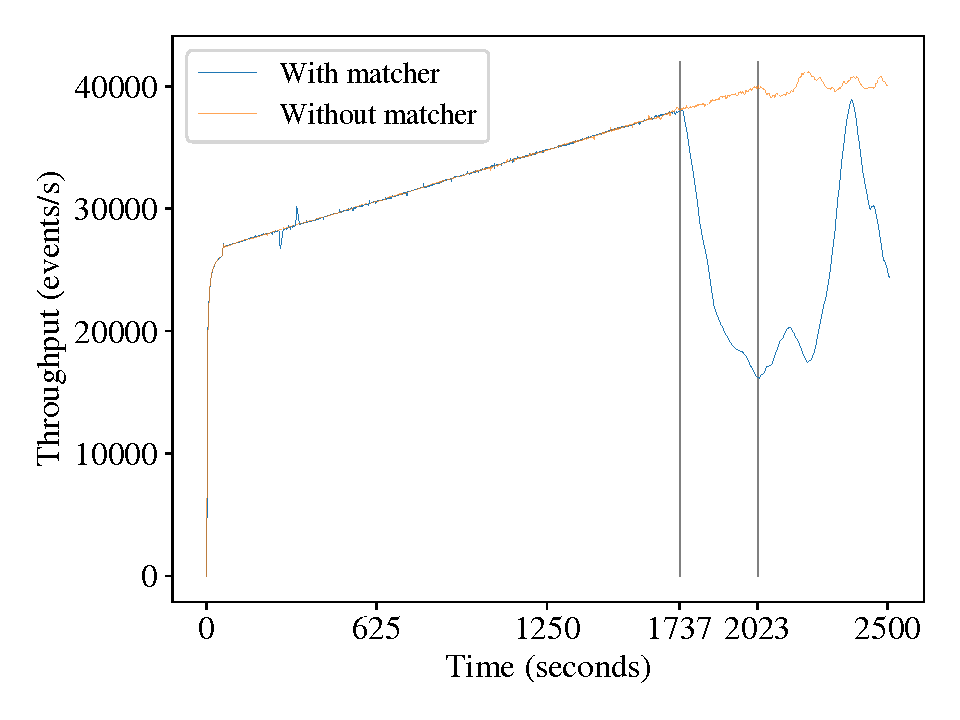
\includegraphics[width=1.0\textwidth]{figures/diffstream/throughput-accelerated.pdf}
        \caption{}\label{diffstream:fig:throughput}
    \end{subfigure}%
    \begin{subfigure}[t]{0.33\textwidth}
        \centering
        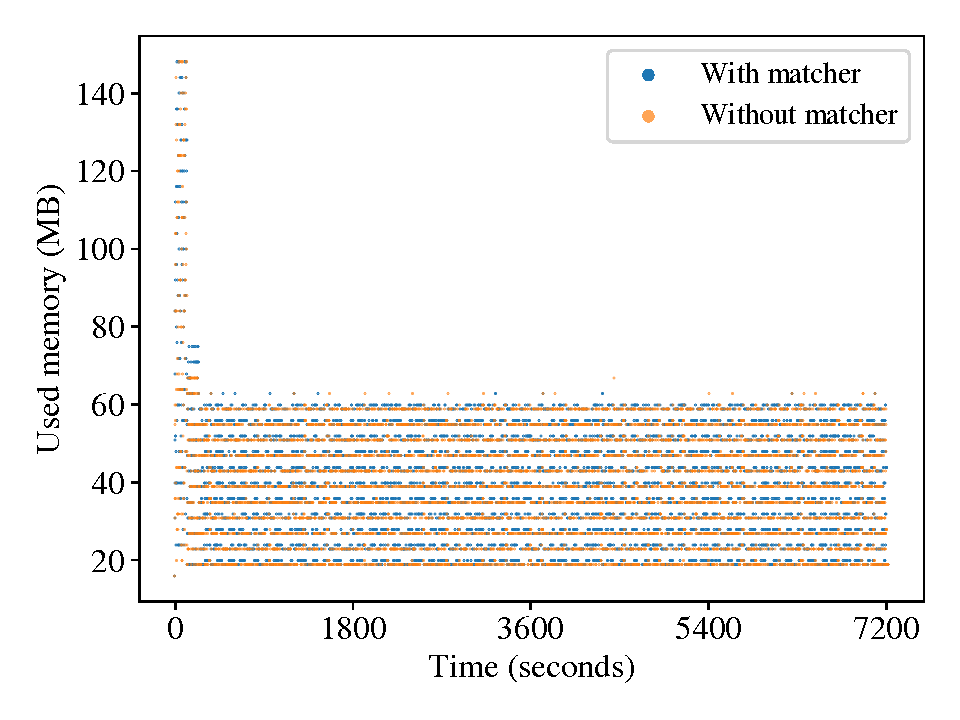
\includegraphics[width=1.0\textwidth]{figures/diffstream/used_memory_in_time.pdf}
        \caption{}\label{diffstream:fig:memory-in-time}
    \end{subfigure}%
    \begin{subfigure}[t]{0.33\textwidth}
        \centering
        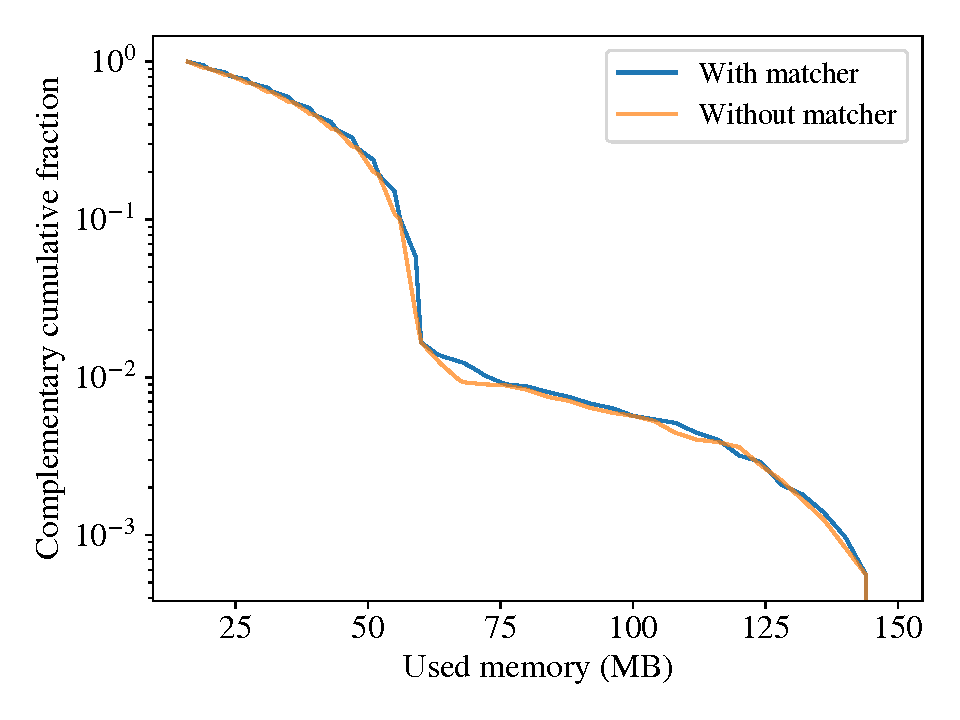
\includegraphics[width=1.0\textwidth]{figures/diffstream/memory_ccdf.pdf}
        \caption{}\label{diffstream:fig:memory-ccdf}
    \end{subfigure}%
    \\
    \begin{subfigure}[t]{0.33\textwidth}
        \centering
        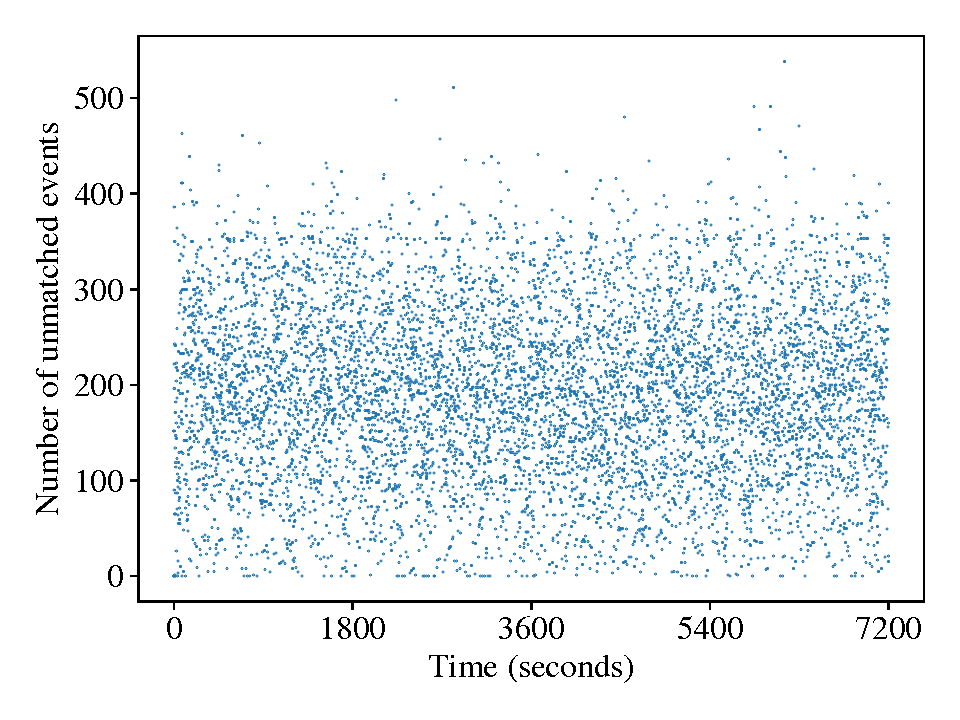
\includegraphics[width=1.0\textwidth]{figures/diffstream/unmatched_in_time.pdf}
        \caption{}\label{diffstream:fig:unmatched-in-time}
    \end{subfigure}%
    \begin{subfigure}[t]{0.33\textwidth}
        \centering
        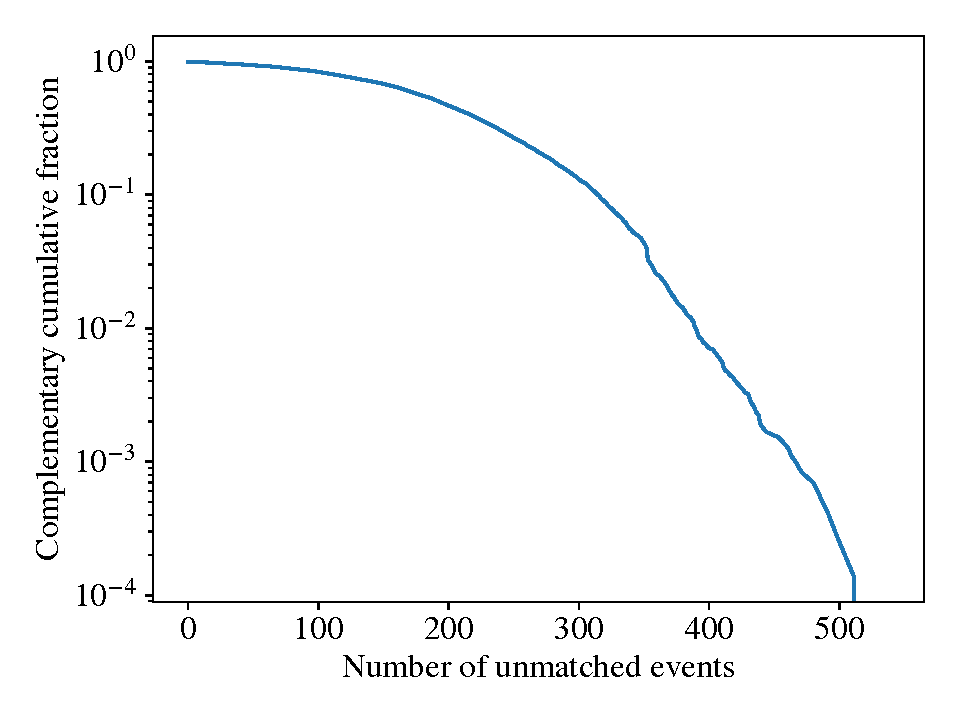
\includegraphics[width=1.0\textwidth]{figures/diffstream/unmatched_ccdf.pdf}
        \caption{}\label{diffstream:fig:unmatched-ccdf}
    \end{subfigure}%
    \begin{subfigure}[t]{0.33\textwidth}
        \centering
        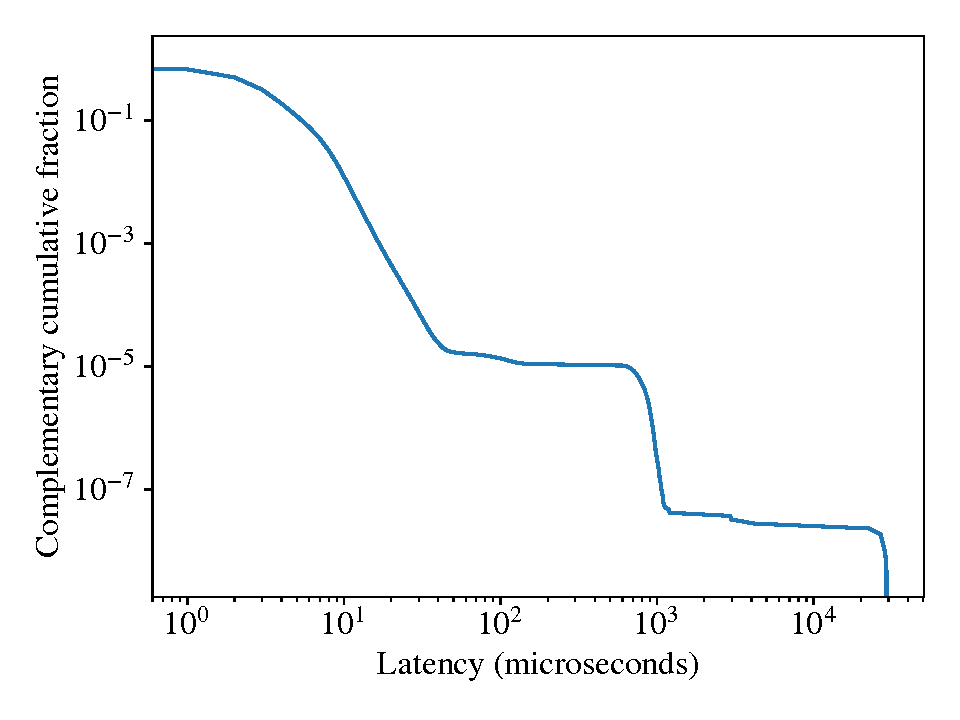
\includegraphics[width=1.0\textwidth]{figures/diffstream/latencies.pdf}
        \caption{}\label{diffstream:fig:latencies}
    \end{subfigure}
    \caption[Performance case study results (Yahoo streaming benchmark).]{Results of the fourth case study: performance measurements of monitoring an application with DiffStream on the Yahoo streaming benchmark over a span of 2 hours, compared to the same application without the DiffStream matcher.}
\label{diffstream:fig:online-perf-results}
\end{figure}

To answer Q1, we modified the ad event producer to steadily increase
the input rate over time. We then executed two experiments: one with the
matcher and one without it. (We simulated the absence of the
matcher with a dummy matcher that ignores every event.) Both
experiments started with an input rate of 40,000 events/s and
the acceleration of 10 events/s$^2$ and ran for 2,500 seconds, allowing the
input rate to increase to 65,000 events/s. The expected ideal throughput of
the matcher is $2/3$ of the input rate due to (i) the duplication
for the two versions of the program, and (ii) the filtering step, which filters
approximately $2/3$ of the events and leaves $1/3$ that finally reach
the matcher. The measured throughput is shown in \Cref{diffstream:fig:throughput}.
Initially, in both experiments the measured throughput matches the ideal
throughput. After 1,737 seconds, the experiment with the matcher reaches
the throughput of 38,072 events/s, after which it rapidly drops and starts
fluctuating. In the experiment without the matcher, the throughput continues
to rise with the input rate until it reaches 40,082 events/s after 2,023 seconds,
after which it also starts fluctuating. Thus, using the matcher results in
approximately 5\% decrease in the maximal throughput.

To answer Q2 and Q3, we implemented a rudimentary memory profiler
that outputs the total heap memory used by the Java Virtual Machine running
the Flink program in 1-second intervals. In addition, we measured the
latencies of the matcher by measuring the time it takes to process each
event; we stored the latencies in a file during execution. We executed
two experiments, with and without the matcher, with a constant input rate
of 45,000 events/s and the duration of 7,200 seconds (2 hours). The input
rate of 45,000 events/s translated into the throughput of 30,000 events/s,
which was stable during the execution.

\Cref{diffstream:fig:memory-in-time} shows a scatter plot of the memory samples taken
during execution. In particular, the total memory used by the program
stays bounded throughout the duration of the experiment. \Cref{diffstream:fig:memory-ccdf}
visualizes the same information in a different way: for an amount of used
memory $x$ on the $x$-axis, the corresponding value on the $y$-axis is
the fraction of memory samples that exceed $x$. The two figures together
show that there is virtually no difference in the memory usage in the two
experiments.
We get a more fine-grained view if we look at the number of unmatched events
that the matcher stores during execution. \Cref{diffstream:fig:unmatched-in-time} shows
a scatter plot of samples of unmatched events taken in 1-second intervals
during execution. In particular, in almost all samples, the number of unmatched
events is below 500. This is even more clearly illustrated in
\Cref{diffstream:fig:unmatched-ccdf}, which shows the fraction of samples exceeding
the given number of unmatched events. Thus, to answer Q2, the memory
footprint of the matcher is bounded and negligible relative to the memory
used otherwise and the throughput of 30,000 events/s.

Finally, to answer Q3,
\Cref{diffstream:fig:latencies} shows the fraction of recorded latencies
that exceed a given number of microseconds.
The mean latency is 2 microseconds.
While the maximal latency is 30 milliseconds, this is rare:
$98.77\%$ of latencies
are at most 10 microseconds, and $>99.99\%$ of latencies are at most
100 microseconds.

\emph{Summary.} The results show that the overhead of running DiffStream in practice is low.
First, the matcher results in a modest $5\%$ reduction in maximal throughput.
Second, the memory usage is stable over time and reflects the theoretical optimality for applications where drift between the two streams is bounded:
the number of unmatched elements is $<1.67\%$ compared to the number events that it processes.
Finally, the latency of the matcher is at most 100 microseconds in $>99.99\%$ of cases, which competitively meets streaming performance standards.

\section{Discussion}
\label{diffstream:sec:conclusion}

As presented, the input to DiffStream consists of the two programs as well as
a \emph{dependence relation} which is used to describe which output
events must be produced in order, and an optional custom equality
which is used to compare output events.
It is also possible to view DiffStream as being a runtime assertion checker: it checks assertions of the form
\[
\texttt{assert s1 == s2}
\]
where \texttt{s1} and \texttt{s2} are streams of a given stream type $S$, and $==$ is stream equivalence $\equivtype{s_1}{s_2}{S}$. Moreover, it does this as efficiently as possible in a streaming complexity sense.

This is how I like to view the library today; an online stream diff calculator. Given a generator and two versions of the program under test, asserting stream equality on their outputs is the usual use case for DiffStream. However, there are other use cases for an equality test, such as validating that a result stream computed by two different nodes is the same.

Keeping in mind the stream-diff-calculator view, here are some possibilities for extension that I currently think would be promising:
\begin{itemize}
  \item First, the library could be extended not just to check equality (yes or no answer), but to truly compute a diff between the two streams. The core algorithmic problem would be more challenging.
  \item Second, the algorithm could be revised to avoid the worst-case behavior described in \Cref{diffstream:sec:practical-bounds} if we relax a simple requirement: if we require that differences between the two streams are detected \emph{with high probability}, rather than necessarily. In particular, one could make use of hash functions for this purpose. Consider the failure case where the two input streams are bags. Rather than store the full diff of the input streams, could one just store a sum of the hash values of each bag? It is mathematically rare for $\sum_{s \in S_1} \texttt{hash}(s) = \sum_{s \in S_2} \texttt{hash}(s)$ unless $S_1 = S_2$.
\end{itemize}

An honest limitation of DiffStream is that it focuses on bugs due to parallelism. In fact, this is only a small class of all bugs; and even smaller if we exclude bugs that could be caught through unit testing without requiring nontrivial dependence relations. In future work, it would be prudent to target other classes of bugs, including those due to node or network faults.
Additionally, we would like to generalize the definition of correct behavior, which currently assumes that the output should be determined up to allowed reordering and equality of data items. There are cases where this is too strong, for instance when operations are approximate or randomized.

Another limitation of DiffStream is that it does not address the problem of input data generation, but instead uses an off-the-shelf generator (JUnit-QuickCheck).
There is an interesting problem of generating input streams of a type $S$,
taking into account the type of $S$, which we don't really consider in this work.
To clarify, DiffStream does check for type safety and determinism, but only on a specific example trace at a time. That is, on an input stream and an equivalent input stream, it can check whether the outputs are equivalent.
But, as with all runtime testing techniques, this only allows testing finitely many input traces.
This is the reason for the \Partial{} entries in \Cref{fig:operator-properties-chapter-table}.

DiffStream is open source and is available \githubref{https://github.com/fniksic/diffstream}{on GitHub}.

\section{Performance Bounds}
\label{sec:monitoring}

In this section we describe data transducers,
an intermediate representation for modeling
stream processing operators as finite state transducers
over data words~\citeMain{icalp17,popl19,tcs20}.
Data transducers support succinct constructions, making them
compositional.
We also describe the QRE-Past monitoring language, which
can be used for monitoring stream processing applications.

\subsection{Motivation}

Applications ranging from network traffic engineering to runtime monitoring of autonomous control systems
require computation over data streams in an efficient and incremental manner.
Declarative programming is a particularly appealing approach to specify the desired logic in such
applications as it can provide natural and high-level constructs for processing streaming data
with guaranteed bounds on computational resources used by the compiled implementation.
This has motivated the development of a number of declarative query languages.
For example, in runtime verification, a monitor observes a sequence of events produced by
a system, and issues an alert when a violation of a safety property is detected, where the safety property
is described in a temporal logic with past-time operators such as \emph{always-in-the-past} and \emph{since}
~\cite{manna2012temporal,havelund2004efficient}.
In quantitative monitoring, a monitor associates a numerical value with an input stream of data values,
where the desired computation is described using \emph{quantitative regular expressions} (QREs) that combine
regular patterns with numerical aggregation operations such as min, max, sum, and average~\cite{AFR2016QRE,MRAIK2017SQRE,YLMMAL2017NQRE}.
In each such case, the declarative specification is automatically compiled into a monitor that
adheres to the streaming model of computation~\cite{M2005DS}: memory and per-item
processing time is polynomial in the size of the specification of the query and, roughly speaking,
does not grow with the length of the input stream.

In existing query languages over streaming data, while a programmer can specify the desired computation
in a modular fashion using constructs of the query language, the compiler generates monolithic code for
a given query.
What is lacking though is an intermediate representation for streaming computations
that supports composition operations with succinct constructions so that high-level queries can be
compiled modularly. The motivation for such a model is two-fold. From a practical viewpoint,
it can facilitate the design of new query languages. For instance, suppose a user wants
to specify a monitoring property using past-time temporal logic, where the atomic
predicates involve comparing quantitative summaries defined using QREs.
Such a specification contains combinators from two different languages (QREs and past-temporal logic), and we could try to design a compiler from scratch for streaming evaluation of the more expressive, integrated language.
However, if we have a \emph{modular} compilation algorithm for the combinators of the two component languages, we get a compiler for the integrated language for free.
From a theoretical viewpoint, designing such a representation is a technical challenge since
it needs to support both combining values from parallel threads of computation (i.e. parallel composition) and unambiguous regular parsing.
In particular, although QREs can be compiled into quantitative automata known
as \emph{cost register automata}~\cite{AdADRY2013CRA}, since this compilation has provably exponential lower bound,
it is not employed by current QRE evaluation algorithms, and in fact, no existing formalism can support
modular compilation of QREs.
The main contribution of this paper is the model of \emph{Data Transducers} (DT) as this desired
modular intermediate representation for streaming computations.

A data transducer processes a data stream---a sequence of tagged data values---and produces
a numerical (or Boolean) value using a fixed set of data variables that are updated
using a constant number of operations as it processes each tagged data value.
A DT can be viewed as a quantitative generalization of (unambiguous) NFAs.
Whereas an NFA configuration consists of a finite set of states, each of which is either inactive or active, % wording change
a DT configuration consists of a finite set of data variables, each of which can be inactive (\emph{undefined}), active
with a value (\emph{defined}), or in a special ``conflict'' mode (\emph{conflicted}).
A DT configuration thus consists of succinctly represented finite control integrated with data values.
As a DT computes by consuming tagged data values, it updates its variables using a specified allowed
set of operations. The values of defined variables can be combined using operations to form new values,
but there is also the possibility of a ``collision''.
This is analogous to how two tokens of active NFA states can be merged into one token
during evaluation when they are placed on the same state. Since the merging of data values
is not in general a meaningful operation, a collision of values results in a variable being set
to conflict.
Since multiple transitions can write to the same data variable while processing a single tagged data value,
and the updated value of a variable can depend on the updated values of the others,
the semantics is defined using fixed points.
We show how this semantics can be implemented
by an efficient streaming algorithm for evaluation that executes a linear (in the size of DT) number
of data operations while processing each tagged data value.

The language of a DT, i.e. the set of stream histories for which its output is defined,
is a regular language over the tags of the input stream.
In fact, DTs capture a robust class of functions with an elegant logical
characterization: MSO-definable string-to-DAG % condensed to save space
transformations with a special ``no backward edges'' requirement. % added...not sure
This class, which we call \emph{streamable regular transductions}, has been studied in
\cite{EM1999MTT,C1994MSOGT,arXiv2018}, and the closure properties of this class, as opposed to some specific constructs supported by
query languages in the existing literature, guide the choice of operations over
DTs for which we seek succinct constructions. % replaced (hopefully succinct) -> succinct

In particular, we show that DTs are closed under
quantitative concatenation, quantitative iteration, union, and parallel composition operations,
and that the corresponding constructions are succinct.
We also consider the \emph{prefix-sum} operation that combines the outputs on all prefixes using
a specified aggregator; this also has a simple and succinct construction on DTs.
Temporal operators such as ``always in the past'', ``sometime in the past'', and ``since'' can be
implemented using prefix-sum.
The design choices in the precise formal definition of the model turn out to be critical in these constructions.
A key restriction on DTs, which we call \emph{restartability}, that is required
for constructions related to unambiguous parsing is identified.
This restriction says that it is possible to ``restart'' the automaton during
a computation by placing new data values at its initial states.
Then, although we only need to store a single automaton configuration in memory, the output is the same as if multiple copies of the automaton were computing
independently on multiple stream suffixes as long as only one of these copies ultimately contributes to the final output.
This ability is necessary for efficient unambiguous parsing: several parsing possibilities
are explored simultaneously, but the required space is constant.

To illustrate the benefits of modular compilation, we define a new query language, called QRE-Past,
that combines the features of past-time temporal logic and QREs.
We specify a cardiac arrhythmia detection algorithm~\cite{AAMMR2018,ZI2016ICD} in QRE-Past to illustrate how
the combination of features leads to a natural high-level specification.
The theory of DTs immediately leads to a streaming evaluation algorithm for QRE-Past,
since every construct in QRE-Past maps to a corresponding construction on component DTs without
causing blow-up.
In fact, there is nothing sacred about QRE-Past: the designer of a high-level
query language over streaming data for a specific domain can introduce new combinators,
in addition to the ones in this paper, as long as there are corresponding succinct constructions
on the low-level model of DTs.

Finally, while there are existing models
with identical expressiveness, DTs are exponentially more succinct (for instance, compared
to unambiguous cost register automata). To gain a better understanding of the
expressiveness and succinctness of DTs,
consider a (generic) streaming algorithm that maintains a fixed number of Boolean and data
variables, and processes each tagged data value by updating these variables by executing a loop-free
code. While such algorithms capture \emph{all} streaming computations, the class of all streaming
computations is not suitable for modular specifications.
For instance, consider the quantitative concatenation operation:
given transductions $f$ and $g$, and a binary data operation ${\textit{op}}$,
$h={\textit{split}}(f,g,{\textit{op}})$ splits the inputs stream $w$ uniquely into two parts $w=w_1w_2$ and
returns $h(w)={\textit{op}}(f(w_1),g(w_2))$.
While DTs are closed under this operation, the class
of all streaming algorithms is not.
We can enforce regularity of a generic streaming algorithm by requiring, for instance, that the updates to the Boolean
variables are not influenced by the values of the data variables. We show that streaming algorithms
with these restrictions can be translated to DTs without any blow-up, thus establishing that
DTs are the most succinct (up to a constant factor) representation of streamable regular transductions.
The structure of a DT---as variables ranging over undefined/defined/conflict values and update code as a set
of transitions of a particular form, as opposed to traditional loop-free update code---not only enforces regularity, but is also what allows us to define succinct constructions
on the representation.

\paragraph*{Outline of section.}
\S\ref{dt:sec:model} introduces the model of data transducers with illustrative examples.
In \S\ref{dt:sec:constructions} we consider a number of semantic operations with
corresponding succinct constructions on DTs, and we define and study the key property of restartability
necessary for some of them.
In \S\ref{dt:sec:rm}, we define the query language QRE-Past, and show how constructions on DTs
immediately yield modular compilation into a streaming evaluation algorithm.
We also show how QRE-Past is useful in specifying a cardiac arrhythmia
detection algorithm. % in a succinct and high-level manner.
\S\ref{dt:sec:succinctness} discusses the expressiveness and succinctness of DTs compared to cost register automata, to finite automata, and to general streaming computations. We compare with related work in
\S\ref{dt:sec:related}, and conclude in \S\ref{dt:sec:conclusions}.

\subsection{Data Transducers}
\label{dt:sec:model}
\label{dt:subsec:preliminaries}

To model data streams we use \emph{data words}.
Let $\data$ be a (possibly infinite) set of \defn{data values},
such as the set of integers or real numbers,
and let $\Sigma$ be a finite set of \defn{tags}.
Then a \defn{data word} is a sequence of tagged data values
$\dw{w} \in (\Sigma \times \data)^*$.
We write $\dw{w} \downarrow \Sigma$ to denote
the projection of $\dw{w}$ to a string in $\Sigma^*$.
We use bold $\dw{u}$, $\dw{v}$, $\dw{w}$ to denote data words.
We reserve non-bold $u, v, w$ for plain strings of tags in $\Sigma^*$.
We write $d, d_i$ for elements of $\data$.
We use $\sigma$ to denote an arbitrary tag in $\Sigma$,
and in the examples we write particular tags in typewriter font, e.g. $\tg{a}, \tg{b}$.

A \defn{signature} is a tuple $(\data, \ops)$,
where $\data$ is a set of data values
and $\ops$ is a set of \defn{allowed operations}.
Each operation has an \defn{arity} $k \ge 0$
and is a function from $\data^k$ to $\data$.
We use $\ops_k$ to denote the $k$-ary operations.
For instance, if $\data$ is all 64-bit integers, we might support 64-bit arithmetic, as well as
integer division and equality tests.
Alternatively we might have $\data = \mathbb{N}$
with the operations $+$ (arity 2), $\min$ (arity 2), and $0$ (arity 0).
In general, we may have arbitrary user-defined operations on $\data$.
Given a signature $(\data, \ops)$,
and a collection of variables $Z$,
the set of \defn{terms} $\tms[Z]$
consists of all syntactically correct expressions
with free variables in $Z$, using operations $\ops$.
So $\min(x,0) + \min(y,0)$ and $x + x$
are terms over the signature $(\mathbb{N}, \{+,\min,0\})$ with $Z = \{x,y\}$.

We define two special values in addition to
the values in $\data$: $\bot$ denotes \defn{undefined}
and $\top$ denotes \defn{conflict}.
We let $\cdata := \data \cup \{\bot, \top\}$ be the set of \defn{extended data values},
and refer to elements of $\data$ as \defn{defined}.
We lift $\ops$ to operations on $\cdata$ by thinking of $\bot$ as the empty multiset,
elements of $\data$ as singleton multisets, and $\top$ as any multiset of two or more data values.
The specific behavior of $\op \in \ops$ on values in $\cdata$
is illustrated in the table below
for the case $\op \in \ops{}_2$.
We also define a \defn{union} operation $\sqcup: \cdata \times \cdata \to \cdata$:
if either of its arguments is undefined it returns the other one,
and in all other cases it returns conflict.
This represents multiset union. Note that $d_1 \sqcup d_2 = \top$ even if $d_1 = d_2$.
This is essential: it guarantees that for all operations on extended data values, whether the result is undefined, defined, or conflict can be determined from knowing only whether the inputs are undefined, defined, or conflict.
%% TODO maybe bring back?
% For instance, we rely on this guarantee for the theorems in
% \S\ref{dt:subsec:dt-regularity} and for the translation from QRE-Past in \S\ref{dt:subsec:rm-compilation}. It's not needed for most of the constructions in \S\ref{dt:sec:constructions}.
\[
\small
\begin{array}{c|ccc}
\sqcup & \bot & d_2 & \top \\
\hline
\bot & \bot & d_2 & \top \\
d_1 & d_1 & \top & \top \\
\top & \top & \top & \top
\end{array}
\qquad \qquad
\begin{array}{c|ccc}
\op & \bot & d_2 & \top \\
\hline
\bot & \bot & \bot & \bot \\
d_1 & \bot & \hspace{-5pt}\op(d_1,d_2)\hspace{-5pt} & \top \\
\top & \bot & \top & \top
\end{array}
\]

$\cdata$ is a \emph{complete lattice}, partially ordered under the
relation $\le$ which is defined by $\bot \le d \le \top$ for all $d \in \data$,
and distinct elements $d, d' \in \data$ are incomparable.
For a finite set $X$, we write the set of functions $X \to \cdata$ as $\cdata^X$; its elements are un-tagged \defn{data vectors}, denoted $\dv{x}$, $\dv{y}$.
The partial order extends coordinate-wise to an ordering $\dv{x} \le \dv{y}$ on data vectors $\dv{x}, \dv{y} \in \cdata^X$.
All operations in $\ops{}$ are \emph{monotone increasing}
w.r.t. this partial order.
Union ($\sqcup$) is commutative and associative, with identity $\bot$ and absorbing element $\top$,
and \emph{all} $k$-ary operations distribute over it.

%%%%%%%%%%%%%%%%%%%%%%%%%%%%%%%%%%%%%%%%%%%%%%%%%%%

\paragraph*{Syntax.}
Let $(\data, \ops)$ be a fixed signature.
A \defn{data transducer (DT)} is a 5-tuple $\DT = \DTtuple$, where:
\begin{itemize}
\item $\states$ is a finite set of \defn{state variables} (\defn{states} for short) and $\tags$ is a finite set of \defn{tags}.
We write $\states'$ for a copy of the variables in $\states$: for $q \in \states$, $q' \in \states'$ denotes the copy. When the states of the DT are updated, $q'$ will be the new, updated value of $q$.
\item $\update$ is a finite set of \defn{transitions},
where each transition is a tuple $(\sigma, X, q', t)$.
\begin{itemize}
\item $\sigma \in \Sigma \cup \{\tg{i}\}$,
where $\tg{i} \notin \Sigma$, and if $\sigma = \tg{i}$ this is a special \emph{initial transition}.
\item $X \subseteq \states \cup \states'$ is a set of
\emph{source variables} and $q' \in \states'$ is the \emph{target variable}.
\item $t \in \tms[X \cup \{\curritem\}]$ gives a new value of the target variable given values of the source variables
and given the value of ``$\curritem$'', which represents the current data value in the input data word.
Assume that $\curritem \notin X$.
We allow $X$ to include some variables not used in $t$.
For initial transitions, we additionally require that $X \subseteq \states'$ and that $\curritem$ does not appear in $t$.
\end{itemize}
\item $\init \subseteq \states$ is a set of \emph{initial states} and $\final \subseteq \states$ is a set of \emph{final states}.
\end{itemize}

The \defn{number of states} of $\DT$ is $|\states|$.
The \defn{size} of $\DT$ is the the number of states plus the total length of all transitions
$(\sigma, X, q', t)$, which includes the length of description of all the terms $t$.

\label{dt:subsec:dt-semantics}

\paragraph*{Semantics.}
The input to a DT has two components.
First, an \defn{initial vector} $\dv{x} \in \cdata^\init$, which assigns an extended data value to each initial state. Second, an \defn{input data word} $\dw{w} \in (\Sigma \times D)^*$, which is a sequence of tagged data values to be processed by the transducer. On input $(\dv{x},\dw{w})$, the DT's final \defn{output vector} is an extended data value at each of its final states.
Thus, the semantics of $\DT$ will be
\[
\sem{\DT} : \cdata^\init \times (\tags \times \data)^* \to \cdata^\final.
\]

A \defn{configuration} is a vector $\dv{c} \in \cdata^\states$.
For every $\sigma \in \Sigma$, the set of transitions $(\sigma, X, q', t)$
collectively define a function $\update_\sigma : \cdata^\states \times \data \to \cdata^\states$:
given the current configuration and the current data value from the input data word,
$\update_\sigma$ produces the next configuration.
We define $\update_\sigma(\dv{c},d)(q) := \dv{c}'(q')$,
where $\dv{c}' \in \cdata^{Q \cup Q' \cup \{\curritem\}}$ is the \emph{least vector} satisfying
$\dv{c}'(\curritem) = d$; for all $q \in Q$, $\dv{c}'(q) = \dv{c}(q)$;
and
\begin{equation}
\text{for all }q' \in Q',\quad
\dv{c}'(q') = \bigsqcup_{(\sigma, X, q', t) \in \update} \sem{t}(\dv{c}'|_X),
\label{dt:eq:fixpoint-semantics}
\end{equation}
where we define $\sem{t}(\dv{c}'|_X)$ to be $\bot$ if there exists $x \in X$ such that $\dv{c}'(x) = \bot$; otherwise, $\top$ if there exists $x \in X$ such that $\dv{c}'(x) = \top$; otherwise, if all variables in $X$ are defined, then $\sem{t}(\dv{c}'|_X)$ is the value of the expression $t$ with variables assigned the values in $\dv{c}'$.
So, $\sem{t}(\dv{c}'|_X)$ produces $\bot$ or $\top$ if some variable in $X$ is $\bot$ or $\top$.
The above union is over all transitions with label $\sigma$ and target variable $q'$.
Since $\cdata$ is a complete lattice, this least fixed point exists by the Knaster-Tarski theorem.

The case of initial transitions ($\update_\tg{i}$) is slightly different. The purpose of initial transitions is to compute an initial configuration $\dv{c}_0 \in \cdata^{\states}$, given the initial vector $\dv{x} \in \cdata^\init$. There is no previous configuration, and no current data value, which is why we required $X \subseteq \states'$ for initial transitions and $\curritem$ was not allowed.
We define the function $\update_\tg{i}: \cdata^\init \to \cdata^\states$ with the same fixed point computation from Equation~\eqref{eq:fixpoint-semantics}, except that the initial states are additionally assigned values given by the vector $\dv{x}$. Define that $\dv{x}(q) = \bot$ if $q \notin \init$. Then define $\update_\tg{i}(\dv{x}) = \dv{c}'$, where $\dv{c}'$ is the \emph{least vector} satisfying, for all $q \in Q$,
$\dv{c}'(q') = \dv{x}(q) \sqcup \bigsqcup_{(\tg{i}, X, q', t) \in \update} \sem{t}(\dv{c}'|_X).$

Now $\DT$ is evaluated on input
$(\dv{x}, \dw{w}) \in \cdata^\init \times (\Sigma \times \data)^*$
by starting from the initial configuration and applying the update functions in sequence as illustrated in
Figure~\ref{dt:fig:dt-eval-illustration}.
Finally, the output $\dv{y} \in \cdata^\final$ is given by $\dv{y} = \dv{c}|_{\final}$, the projection of $\dv{c}$ to the final states.

\begin{figure}[t]
\centering \small
\tikzset{>=stealth',auto,semithick,
        node distance=0.8cm,
        square/.style={draw,inner sep=0pt,fill=white,
        regular polygon,regular polygon sides=4,minimum size=25pt}}
%% Background layer
\pgfdeclarelayer{bg}
\pgfsetlayers{bg,main}
\begin{tikzpicture}[scale=0.8]
%%%
\node (x1) at (-1.5,0.2) {$x_1$};
\node (x2) at (-1.5,-0.2) {$x_2$};
\node (y) at (10,0) {$y$};
\node[square] (i) at (0,0) {$\update_\tg{i}$};
\node[square] (1) at (2,0) {$\update_\tg{a}$};
  \node[draw=none] (d1) at (2,1.1) {$d_1$};
\node[square] (2) at (4,0) {$\update_\tg{b}$};
  \node[draw=none] (d2) at (4,1.1) {$d_2$};
\node[square] (3) at (6,0) {$\update_\tg{a}$};
  \node[draw=none] (d3) at (6,1.1) {$d_3$};
\node[square] (4) at (8,0) {$\update_\tg{a}$};
  \node[draw=none] (d4) at (8,1.1) {$d_4$};
% Edges
\draw[->] (x1) -- (i);
\draw[->] (x2) -- (i);
\draw[->] (4) edge node {$\dv{c}_4$} (y);
%%%
\draw[->] (d1) -- (1);
\draw[->] (d2) -- (2);
\draw[->] (d3) -- (3);
\draw[->] (d4) -- (4);
%%
\draw[->] (i) edge node {$\dv{c}_0$} (1);
\draw[->] (1) edge node {$\dv{c}_1$} (2);
\draw[->] (2) edge node {$\dv{c}_2$} (3);
\draw[->] (3) edge node {$\dv{c}_3$} (4);
\end{tikzpicture}
\caption{Example evaluation of a data transducer $\DT$ with two initial states and one final state on initial vector $(\dv{x}_1, \dv{x}_2)$ and an input data word $\dw{w}$ consisting of four characters (tagged data values):
$(\tg{a},d_1)$, $(\tg{b},d_2)$, $(\tg{a},d_3)$, $(\tg{a}, d_4)$, to produce output $y$.
Here $\dv{c}_0, \dv{c}_1, \dv{c}_2, \dv{c}_3$, and $\dv{c}_4$ are configurations; $d_i \in \data$; and $x_1, x_2, y \in \cdata$. Each $\Delta_\sigma$ is a set of transitions, collectively describing the next configuration in terms of the previous one.}
\label{dt:fig:dt-eval-illustration}
\end{figure}

\paragraph*{Evaluation Complexity.}
Evaluation complexity of a data transducer depends on the underlying
operations, so we give a conditional result where the complexity
is stated in terms of the number of data registers and number of
operations on those data registers.

\begin{theorem}
Evaluation of a data transducer $\DT$, with number of states $n$ and size $m$ on input $(\dv{x},\dv{w})$, requires
$O(n)$ data registers to store the state,
and $O(m)$ operations and additional data registers
to process each element in $\tags \times \data$, independent of $\dv{w}$.
The evaluation algorithm is given in Figure~\ref{dt:fig:dt-eval-algorithm}.
\label{dt:thm:dt-eval}
\end{theorem}

\begin{figure}[t]
\vspace{-8pt}
\centering \footnotesize
\begin{algorithmic}

\State $\dv{c} \gets \update_{\tg{i}}(\dv{x})$; produce output $\dv{y} = \dv{c}|_{\final}$

\For{each character $(\sigma,d)$ in $\dv{w}$}
    \For{each state $q \in Q$}
        $\mathit{val}(q) \gets \dv{c}(q)$;
        $\mathit{val}(q') \gets \bot$
    \EndFor
    \For{each transition $\tau \in \update_\sigma$}
        $\mathit{val}(\tau) \gets \bot$;
        $\mathit{num\_undef}(\tau) \gets |X|$
    \EndFor
    \State $\mathit{worklist} \gets Q' \cup \update_\sigma$
    \While{$\mathit{worklist}$ is nonempty, \textbf{get} $\mathit{item}$ from $\mathit{worklist}$ and}
        % \State $\mathit{item} \gets \mathit{worklist}.\texttt{pop()}$
        \If{$\mathit{item}$ is a transition $\tau = (\sigma, X, q', t) \in \update_\sigma$:}
            \State $\mathit{val}(\tau) \gets \sem{t}(\mathit{val}|_X)$
            \If{$\mathit{val}(q') \ne \top$}
                add $q'$ to $\mathit{worklist}$
            \EndIf
        \ElsIf{$\mathit{item}$ is a state $q' \in Q'$}
            \If{$\mathit{val}(q') = \bot$}
                \For{each $\tau \in \update_\sigma$ with source variable $q'$}
                    $\mathit{num\_undef}(\tau) \gets \mathit{num\_undef}(\tau) - 1$
                \EndFor
            \EndIf
            \State $\mathit{val}(q') \gets \bigsqcup_{\tau = (\sigma, X, q', t)} \mathit{val}(\tau)$
            \For{each $\tau \in \update_\sigma$ with target variable $q'$}
                \If{$\mathit{val}(\tau) \in \data$ or ($\mathit{val}(\tau) = \bot$ and $\mathit{num\_undef}(\tau) = 0$)}
                    add $\tau$ to $\mathit{worklist}$
                \EndIf
            \EndFor
        \EndIf
    \EndWhile
    %% Compactified a bit
    % \State $\dv{c} \gets \mathit{val}|_{Q'}$; produce output $\dv{y} = \dv{c}|_{\final}$
    \For{each $q \in Q$}
        $\dv{c}(q) \gets \mathit{val}(q')$
    \EndFor
    \State produce output $\dv{y} = \dv{c}|_{\final}$
\EndFor
\end{algorithmic}
\caption{Data transducer evaluation algorithm (Theorem~\ref{dt:thm:dt-eval}). On input $\DT = \DTtuple$ over $(\data, \ops)$, an initial vector $\dv{x} \in \cdata^\init$, and a data stream $\dv{w} \in (\Sigma \times \data)^*$, produces the output vector $\dv{y} \in \cdata^\final$ on each prefix of $\dv{w}$.
}
\label{dt:fig:dt-eval-algorithm}
\end{figure}

% \subsubsection{Regularity}
\paragraph*{Regularity}
\label{dt:subsec:dt-regularity}
Data transducers define \emph{regular transductions} on data words (see \S\ref{dt:subsec:dts-and-cras}). Here, we show regularity in a simpler sense: whether an output value is defined (or undefined, or conflict) depends only on whether the input values are undefined, defined, or conflict, together with some regular property of the string of tags. For data vectors $\dv{x}_1, \dv{x}_2 \in {\cdata}^X$, we say that $\dv{x}_1$ and $\dv{x}_2$ are \emph{equivalent}, and write $\dv{x}_1 \equiv \dv{x}_2$, if for all $x \in X$, $\dv{x}_1(x)$ and $\dv{x}_2(x)$ are both undefined, both defined, or both conflict.

\begin{theorem}
\label{dt:thm:regular-language}
Let $\DT = \DTtuple$ be a DT over $(\data, \ops)$. Then:
(i) For all initial vectors $\dv{x}_1, \dv{x}_2 \in \data^\init$,
and for all input words $\dw{w}_1, \dw{w}_2$,
if $\dv{x}_1 \equiv \dv{x}_2$ and $\dw{w}_1 \downarrow \Sigma = \dw{w}_2 \downarrow \Sigma$,
then $\sem{\DT}(\dv{x}_1,\dw{w}_1) \equiv \sem{\DT}(\dv{x}_2,\dw{w}_2)$.
(ii) For every equivalence class of initial vectors $\dv{x}$ and equivalence class of output vectors $\dv{y}$, the set of strings $\dw{w} \downarrow \Sigma$ such that $\sem{\DT}(\dv{x},\dw{w}) \equiv \dv{y}$ is regular.
\end{theorem}
\begin{proof}
In evaluating a DT we may collapse all values in $\data$ to a single
value $\one$, so each state takes values in $\{\bot, \one, \top\}$.
This gives a projection from $\DT$ to a DT
$\aut{P}$ over the \defn{unit signature} $(\UU, \Uops)$,
where $\UU = \{\one\}$ is a set with just one element,
and $\Uops$ consists of, for each $k$, the unique
map $\uop_k : \UU^k \to \UU$.
The projection homomorphically preserves the semantics.
Then, (i) follows because the computation of $\aut{P}$ is exactly the same
on $\dv{x}_1, \dw{w}_1$ and $\dv{x}_2, \dw{w}_2$, and (ii) follows because $\aut{P}$ has finitely many possible configurations.
\end{proof}

We can thus define the \defn{language} of $\DT$ to be $\lang(\DT) = \{\dw{w} \downarrow \Sigma \mid \sem{\DT}(\dv{x},\dw{w}) \in \data^\final \text{ for some } \dv{x} \in \data^\init\}$, so $\lang(\DT) \subseteq \Sigma^*$. This is the set of tag strings $\dw{w} \downarrow \Sigma$ such that, if the initial vector of values is all defined, after reading in $\dw{w}$ all final states are defined.
We similarly define the set of strings on which a DT is \emph{defined or conflict}, on input of the same form: the \emph{extended language} $\clang(\DT)$ is
$\{\dw{w} \downarrow \Sigma \mid \sem{\DT}(\dv{x},\dw{w}) \in (\data \cup \{\top\})^\final \text{ for some } \dv{x} \in (\data \cup \{\top\})^\init\}$.
An immediate corollary of Theorem~\ref{dt:thm:regular-language} is that
(i) $\lang(\DT)$ is regular, (ii) $\clang(\DT)$ is regular, and (iii) $\lang(\DT) \subseteq \clang(\DT)$.
Finally, say that DTs $\DT_1$ and $\DT_2$ are \emph{equivalent} if for all $\dv{x}_1 \equiv \dv{x}_2$ and
for all $\dw{w}$, $\sem{\DT_1}(\dv{x}_1,\dw{w}) \equiv \sem{\DT_2}(\dv{x}_2,\dw{w})$.

\begin{theorem}
\label{dt:thm:equivalence-pspace-complete}
On input DTs $\DT_1$, $\DT_2$,
deciding if $\DT_1$ and $\DT_2$ are equivalent is PSPACE-complete.
\end{theorem}
\begin{proof}
We first decide if the two are \emph{not} equivalent in NPSPACE.
It suffices to project $\DT_1$ and $\DT_2$ to DTs
over the unit signature, $\aut{P}_1$ and $\aut{P}_2$, as in the previous proof,
and decide if $\aut{P}_1 \not\equiv \aut{P}_2$.
Let $n$ be the number of states between $\aut{P}_1$ and $\aut{P}_2$,
and let $m$ be their combined size.
The number of configurations for $\aut{P}_1$ and $\aut{P}_2$ together is $3^n$.
Therefore, if there is a counterexample, it is some string over $\Sigma$ of length at most $3^n$.
Guessing the counterexample one character at a time
requires linear in $n$ space to record the count and $O(m)$ space to update
$\aut{P}_1$ and $\aut{P}_2$ (by Theorem~\ref{dt:thm:dt-eval}).

To show it is PSPACE-hard,
it suffices to exhibit a translation from NFAs to
DTs which reduces
language equality of NFAs to equivalence of DTs.
Specifically, we create $\DT$ with one final state
which is undefined on strings for which the NFA is undefined, and $\top$
on strings for which the NFA is defined.
The translation works by directly copying the states and transitions of the NFA, except we add \emph{two} additional transitions from accepting states of the NFA to the new final state of $\DT$.
\end{proof}

\subsection{Constructions}
\label{dt:sec:constructions}

Our primary interest in the DT model is to support a variety of succinct \emph{composition operations} which are not simultaneously supported by any existing model. In particular, such composition operations can enable a quantitative monitoring language like \QREpast{} in \S\ref{dt:sec:rm}: language constructs can be implemented by the compiler as constructions on DTs, rather like how (traditional) regular expressions are compiled to nondeterministic finite automata.

For example, suppose we have DTs implementing two functions $f, g: (\tags \times \data)^{*} \to \cdata$, and we would like to implement the function $f + g$, which applies $f$ and $g$ to the input stream and adds the results.
To do so, we copy the states of the transducers for $f$ and $g$,
and we initialize and update the states in parallel (they do not interfere).
Then, we provide a new final state, and a single new transition which says that the new final state should be assigned the value of the final state of $f$ plus the value of the final state of $g$.
This works for every operation, and not just $+$: the combination of $k$ computations by applying a $k$-ary operation $\op \in \ops_k$ can be implemented by a corresponding $k$-ary construct on the $k$ underlying DTs. Moreover, the size of the DT will only be the sum of the sizes of the $k$ DTs, plus a constant.
In contrast, even this simple operation $f+g$ is not succinctly implementable using the most natural existing alternative to DTs, Cost Register Automata (see \S\ref{dt:sec:succinctness}).

This construction for $f+g$ requires no assumptions about the DTs implementing $f$ and $g$.
However, not all operations are this straightforward.
Consider the following quantitative generalization of concatenation. Given $f: (\Sigma \times \data)^{*} \to \cdata$, $g: (\Sigma \times \data)^{*} \to \cdata$, and $\op \in \ops_2$, we wish to implement $\splitQ(f,g,\op)$:
on input $\dw{w}$, split the input stream into two parts, $\dw{w} = \dw{u} \cdot \dw{v}$, such that $f(\dw{u}) \ne \bot$ and $g(\dw{v}) \ne \bot$ (respectively, $f$ matches $\dw{u}$ and $g$ matches $\dw{v}$), and return $\op(f(\dw{u}),g(\dw{v}))$. Assume that the decomposition of $\dw{w}$ into $\dw{u}$ and $\dw{v}$ such that $f(\dw{u}) \ne \bot$ and $g(\dw{v}) \ne \bot$ is unique.
In order to naively implement this operation, on an input string $\dw{w}$, we must not only keep track of the current
configuration of $f$ on $\dw{w}$,
but for \emph{every} split $\dw{w} = \dw{u} \dw{v}$ where $f$ matches $\dw{u}$,
we must keep track of the current configuration of $g$ on $\dw{v}$.
If there are many possible prefixes $\dw{u}$ of $\dw{w}$ such that $f(\dw{u}) \ne \bot$, we may have to keep arbitrarily many configurations of $g$. This naive approach is therefore impossible using only the finite space that a DT allows, if we treat $f$ and $g$ only as black boxes.
% , whose implementations lack additional structure.
% Indeed, it is possible to give examples of $f$ and $g$ which are efficiently implementable in the streaming setting, whereas $h = f \cdot g$ is not implementable without linear space in the input stream.

What we need to avoid this is an additional structural condition on $g$. Rather than keeping multiple copies of $g$, we would like to keep only a single configuration in memory: whenever the current prefix matches $f$, \emph{restart} $g$ with new data values on its initial states (keeping any current data values as well).
To motivate this idea, consider the analogous concatenation construction for two NFAs: every time the first NFA accepts, we are able to ``restart'' the second NFA by adding a token to its start state (we don't need an entirely new NFA every time).
This property for DTs is called \emph{restartability}.
Restartable DTs are an equally expressive subclass
consisting of those DTs for which restarting computation on the same transducer does not cause interference in the output.

The set of strings that a DT ``matches'' is captured by its \emph{extended language}, defined in \S\ref{dt:subsec:dt-regularity}. Correspondingly, we assume that whenever a DT is restarted, the new initial vector is either all $\bot$, or all \emph{not} $\bot$ (in $\data \cup \{\top\}$). If the \emph{output} of a DT also satisfies this property (on every input it is either all $\bot$, or all \emph{not} $\bot$), then we say that the DT is \emph{output-synchronized}. This property is required in the concatenation and iteration constructions, but it is not as crucial to the discussion as restartability.

We begin in \S\ref{dt:subsec:constructions-general} by giving general constructions that do not rely on restartability. We highlight the implemented semantics, the extended language, and the size of the constructed DT in terms of its constituent DTs.
Then in \S\ref{dt:subsec:constructions-restartable}, we define restartability and use it to give succinct constructions for unambiguous parsing operations, namely \emph{concatenation} and \emph{iteration}.
Moreover, we show that (under certain conditions) our operations \emph{preserve} restartability, thus enabling modular composition using the restartable DTs. We also show that checking restartability is hard (PSPACE-complete), and we mention converting a non-restartable DT to a restartable one, but with exponential blowup.

\subsubsection{General Constructions}
\label{dt:subsec:constructions-general}

\paragraph*{Notation}
It is convenient to introduce shorthand $(\varepsilon, X, q', t)$ for the union of $|\Sigma| + 1$ transitions: $(\sigma, X, q', t)$ for every $\sigma \in \Sigma \cup \{{\tg{i}}\}$. Because this includes an initial transition, this requires that $X \subseteq \states'$ and that $\curritem$ does not appear in $t$. We call such a collection of transitions an \emph{epsilon transition} because, like epsilon transitions from classical automata, the transition may produce a value at its target state on the empty data word and on every input character.

For readability, we abbreviate the type of a DT
$\DT: \cdata^I \times (\Sigma \times D)^* \to \cdata^F$ as $\DT: \DTtype{I}{F}$.
This can be thought of as a function from input variables $I$ of type $\cdata$ to output variables $F$ of type $\cdata$, which also consumes some data word in $(\Sigma \times D)^*$ as a side effect.
For sets of variables (or states) $X_1, X_2$, when we write $X_1 \cup X_2$ we assume that the union is disjoint, unless otherwise stated.

We also define a \emph{data function} to be a plain function $\cdata^I \to \cdata^F$ which is
% equal to some composition of operations in $\ops$. Such a function can be
given by a collection of one or more terms $t : \tms[I]$ for each $f \in F$ (the output value of $f$ is then the union of the values of all terms). If $\DF \subseteq F \times \tms[I]$, then we write $\DF: \DFtype{I}{F}$ to abbreviate the semantics $\sem{\DF}: \cdata^I \to \cdata^F$.
The \defn{size} of $\DF$ is the total length of description of all of the terms $t$ it contains.

\paragraph*{Parallel composition.}
Suppose we are given DTs $\DT_1 = \DTtuplesub{1}$ and $\DT_2 = \DTtuplesub{2}$, and assume that the sets of initial states are the same up to some implicit bijections $\pi_1: I \to I_1$, $\pi_2: I \to I_2$, for a set $I$ with $|I| = |I_1| = |I_2|$. (It is always possible to benignly extend both DTs with extra initial states so that they match, so this assumption is not restrictive.)
We wish to define a DT which feeds the input $(\dv{x},\dw{w})$ into both DTs in parallel. To do so, we define $\DT = \parcompDT{\DT_1}{\DT_2}$ to be the tuple $\DTtuple{}$, where $Q = Q_1 \cup Q_2 \cup I$, $F = F_1 \cup F_2$, and
\begin{align*}
\Delta = \Delta_1 \cup \Delta_2
    \cup \big\{(\varepsilon, i', \pi_1(i)', i') : i \in I \big\}
    \cup \big\{(\varepsilon, i', \pi_2(i)', i') : i \in I \big\}.
\end{align*}
Here, the transitions we added (those in $\Delta$ but not in $\Delta_1$ or $\Delta_2$) \emph{copy} values from $I$ into both $I_1$ and $I_2$. This is only relevant on initialization $\update_{\tg{i}}$, since after that states $I$ will not be defined, but we used an epsilon transition instead of just an ${\tg{i}}$ transition to preserve restartability, which will be discussed in \S\ref{dt:subsec:restartability}. Since we added no other transitions, the least fixed point Equation~\eqref{eq:fixpoint-semantics} defining the next (or initial) configuration decomposes into the least fixed point on states $Q_1$, and on states $Q_2$. It follows that the semantics satisfies $\sem{\DT}(\dv{x},\dw{u}) = (\sem{\DT_1}(\dv{x},\dw{u}),\sem{\DT_2}(\dv{x},\dw{u}))$. Here, $(\dv{y}_1,\dv{y}_2)$ denotes the vector $\dv{y} \in \cdata^F$ that is $\dv{y}_1$ on $F_1$ and $\dv{y}_2$ on $F_2$.
Parallel composition is commutative and associative.
The utility of parallel composition is that it allows us to combine the outputs $\dv{y}_1$ and $\dv{y}_2$ later on. This is accomplished by \emph{concatenation} with another DT which combines the outputs (\S\ref{dt:subsec:constructions-restartable}).

\begin{figure*}[h]
\fbox{\begin{minipage}{.98\textwidth}
\textbf{Parallel composition.}
If $\DT_1: \DTtype{I}{F_1}$ and $\DT_2: \DTtype{I}{F_2}$,
then $\parcompDT{\DT_1}{\DT_2} : \DTtype{I}{F_1 \cup F_2}$ satisfies
% implements the semantics
\[
\sem{\parcompDT{\DT_1}{\DT_2}}(\dv{x},\dw{w}) = (\sem{\DT_1}(\dv{x},\dw{w}),\sem{\DT_2}(\dv{x},\dw{w})),
\]
such that $\size{\parcompDT{\DT_1}{\DT_2}} = \size{\DT_1} + \size{\DT_2} + O(|I|)$.
It therefore matches the set of tag strings
$\clang(\parcompDT{\DT_1}{\DT_2}) = \clang(\DT_1) \cap \clang(\DT_2)$.
\end{minipage}}

\label{dt:fig:parallel-composition}
\end{figure*}

\paragraph*{Union.}
Suppose we are given DTs $\DT_1 = \DTtuplesub{1}$ and $\DT_2 = \DTtuplesub{2}$, and assume that the sets of initial and final states are the same up to some bijections: $\pi_1: I \to I_1$, $\pi_2: I \to I_2$, $\rho_1: F \to F_1$, $\rho_2: F \to F_2$, for sets $I$ and $F$ with $|I| = |I_1| = |I_2|$ and $|F| = |F_1| = |F_2|$. We wish to define a DT which feeds the input $(\dv{x},\dw{w})$ into both DTs in parallel and returns the union $(\sqcup)$ of the two results.
We define $\DT = \union{\DT_1}{\DT_2} = \DTtuple{}$ by $Q = Q_1 \cup Q_2 \cup I \cup F$ and
\begin{alignat*}{2}
\Delta = \Delta_1 \cup \Delta_2
    &\cup \big\{(\varepsilon, i', \pi_1(i)', i') : i \in I \big\}
    &&\cup \big\{(\varepsilon, i', \pi_2(i)', i') : i \in I \big\} \\
    &\cup \big\{(\varepsilon, \rho_1(f)', f', \rho_1(f)') : f \in F \big\}
    &&\cup \big\{(\varepsilon, \rho_2(f)', f', \rho_2(f)') : f \in F \big\}.
\end{alignat*}

Similar to the parallel composition construction, the additional transitions here ensure that we copy values from $I$ into $I_1$ and $I_2$, and copy values from $F_1$ and $F_2$ into $F$, whenever these values are defined. In particular, on initialization the initial vector $\dv{x}$ will be copied into $I_1$ and $I_2$, and on every data word the output values $\dv{y}_1$ and $\dv{y}_2$ of $\DT_1$ and $\DT_2$ will be copied into the \emph{same} set of final states, so that they have to be joined by $\sqcup$. In particular, if both $\dv{y}_1$ and $\dv{y}_2$ are defined, the output will be $\top$. We see therefore that the semantics is such that $\sem{\DT}(\dv{x},\dw{u}) = \sem{\DT_1}(\dv{x},\dw{u}) \sqcup \sem{\DT_2}(\dv{x},\dw{u})$. Like parallel composition, union is commutative and associative.

\begin{figure*}[h]
\fbox{\begin{minipage}{.98\textwidth}
\textbf{Union.}
If $\DT_1: \DTtype{I}{F}$ and $\DT_2: \DTtype{I}{F}$,
then $\union{\DT_1}{\DT_2} : \DTtype{I}{F}$
implements the semantics
\[
\sem{\union{\DT_1}{\DT_2}}(\dv{x},\dw{w}) = \sem{\DT_1}(\dv{x},\dw{w}) \sqcup \sem{\DT_2}(\dv{x},\dw{w}),
\]
s.t. $\size{\union{\DT_1}{\DT_2}} = \size{\DT_1} + \size{\DT_2} + O(|I| + |F|)$.
It matches
$\clang(\union{\DT_1}{\DT_2}) = \clang(\DT_1) \cup \clang(\DT_2)$.
\end{minipage}}

\label{dt:fig:union}
\end{figure*}

\paragraph*{Prefix summation.}
Now we consider a more complex operation. Suppose we are given $\DT_1 = \DTtuplesub{1}$, and a data word $\dw{w}$, such that the output on the empty data word is $\dv{y}^{(0)}_1$, the output after receiving one character of the data word is $\dv{y}^{(1)}_1$, and in general the output after $k$ characters is $\dv{y}^{(k)}_1$. The problem is to return the \emph{sum} of these outputs: we want a DT that returns $\dv{y}^{(i)} = \dv{y}^{(0)}_1 + \cdots + \dv{y}^{(i)}_1$ after receiving $i$ characters. This is called the \emph{prefix sum} because $\dv{y}^{(k)}_1$ is the value of $\DT$ on the $k$th prefix of the data word.
In general, instead of $+$, we can take an arbitrary operation which folds the outputs of $\DT_1$ on each prefix. We suppose that this operation is given by a data function $\DF$ which, for some set $F$, is a function $\cdata^{F \cup F_1} \to \cdata^{F}$. It takes the previous ``sum'' $\dv{y}^{(i-1)} \in \cdata^F$, combines it with the new output of $\DT_1$, $\dv{y}_1^{(i)} \in \cdata^{F_1}$, and produces the next ``sum'' $\dv{y}^{(i)} \in \cdata^F$. So, we'll have $G(\dv{y}^{(i-1)},\dv{y}_1^{(i)}) = \dv{y}^{(i)}$. We want a DT that, on input initial values for $I_1$ and initial values $\dv{y}^{(-1)}$ for $F$, will return $\dv{y}^{(i)}$.
%% Would like to add this space back..
Formally, we convert $\DF$ to a DT $\DT_2 = \DTtuplesub{2}$, with bijections $\pi: (F \cup F_1) \to I_2$, $\rho: F \to F_2$, which only contains epsilon-transitions: for each term $t$ in $G$ with variables $P \subseteq (F \cup F_1)$ giving a value of $f \in F$, we create an epsilon transition $(\varepsilon, \pi(P)', \rho(f)', t)$. Then we define the prefix sum $\prefixsum{\DT_1}{\DF} = (Q, \Sigma, \Delta, (I_1 \cup F), F_2)$, where $Q = Q_1 \cup Q_2 \cup F$ and
\begin{align*}
\Delta = \Delta_1 \cup \Delta_2
    &\cup \big\{(\varepsilon, f_1', \pi(f_1)', f_1') : f_1 \in F_1 \big\} \\
    &\cup \big\{(\varepsilon, f', \pi(f)', f') : f \in F \big\}
    \quad \cup \big\{(\sigma, \rho(f), \pi(f)', \rho(f)) : f \in F, \sigma \in \Sigma \big\}.
\end{align*}

First on the empty data word, the outputs $F_2'$ of $\DT_1$ and the initial vector in $F'$ are copied into $I_2$, and $\DT_2$ produces the correct output $\dv{y}^{(0)} = \sem{\DF}(\dv{y}^{(-1)},\dv{y}_1^{(0)})$. Now, when we read in a character in $\Sigma \times \data$, the final states $F_2'$ flow back into inputs to $\DT_2$, and the new output of $\DT_1$ also flows in. Because the machine $\DT_2$ was constructed to be just a set of epsilon-transitions from $I_2$ to $F_2$, it does not save any internal state, but just computes the output in terms of the input again. So the next output will be $\sem{\DF}(\dv{y}^{(0)},\dv{y}_1^{(1)})$, and then $\sem{\DF}(\dv{y}^{(1)},\dv{y}_1^{(2)})$, and so forth.
% The extended language of matched strings depends on $\DF$; we do not write it out explicitly.

\begin{figure*}[h]
\fbox{\begin{minipage}{.98\textwidth}
\textbf{Prefix sum.}
If $\DT_1: \DTtype{I}{Z}$
and $\DF: \DFtype{F \cup Z}{F}$,
then $\prefixsum{\DT_1}{\DF}: \DTtype{I \cup F}{F}$
implements the semantics
\begin{align*}
\sem{\prefixsum{\DT_1}{\DF}}((\dv{x},\dv{y}),\varepsilon)
    &= \sem{\DF}(\dv{y},\sem{\DT_1}(\dv{x},\varepsilon)) \\
\sem{\prefixsum{\DT_1}{\DF}}((\dv{x},\dv{y}),\dw{w} (\sigma,d))
    &= \sem{\DF}(\sem{\prefixsum{\DT_1}{\DF}}((\dv{x},\dv{y}),\dw{w}),\sem{\DT_1}(\dv{x},\dw{w} (\sigma,d)))
\end{align*}
such that $\size{\prefixsum{\DT_1}{\DF}} = \size{\DT_1} + \size{\DF} + O(|Z| + |F|)$.
\end{minipage}}

\label{dt:fig:prefix-sum}
\end{figure*}

\paragraph*{Conditioning on undefined and conflict values.}
A DT that is constructed using the other operations---particularly union, and concatenation and iteration from \S\ref{dt:subsec:constructions-restartable}---may produce undefined ($\bot$) or conflict ($\top$) on certain inputs. In such a case, we may want to perform a computation which \emph{conditions} on whether the output is undefined, defined or conflict: for instance, we may want to produce $1$ if there is a conflict, or we may want to replace all $\bot$ and $\top$ outputs with concrete data values. (In particular, in \S\ref{dt:sec:rm}, we will want to replace $\bot$ and $\top$ with Boolean values.) We give a construction for this purpose. To simplify the problem, suppose that we are given $\DT_1 = \DTtuplesub{1}$, and we want to construct a DT $\DT_\bot$ with no initial states, the same set of final states, and the following behavior: for all $\dv{x} \in \data^{\init_1}$ (\emph{not} $\cdata^{\init_1}$), all $\dw{u} \in (\Sigma \times \data)^{*}$, and all $f_1 \in \final_1$, if $\sem{\DT_1}(\dv{x},\dw{u})(f_1) = \bot$ then $\sem{\DT_\bot}(\dw{u})(f_1) \in \data$, and otherwise, $\sem{\DT_\bot}(\dw{u})(f_1) = \bot$. Here, since $I = \varnothing$, the first argument is omitted. We similarly want to define $\DT_\data$ which is in $\data$ if $\DT_1$ is in $\data$, and $\bot$ otherwise, and $\DT_\top$ which is in $\data$ if $\DT_1$ is $\top$, and $\bot$ otherwise.
So that $\data$ is not empty, we assume that there is some constant operation in $\ops_0$, say $d_\one$ (so $d_\one \in \data$).

The idea of the construction is that we replace $Q_1$ with $Q_1 \times \{\bot, \one,\top\}$. For each state $q \in Q_1$, at all times, exactly one of $(q, \bot)$, $(q, \one)$, and $(q, \top)$ will be $d_\one$ and the other two will be $\bot$. Which state is $d_\one$ should correspond to whether $q$ was undefined, defined, or conflict. (This is adapted from the classic trick of dealing with negation by replacing all values with pairs of either (true, false) or (false, true).) However, in order for this to work without blowup our DT needs to be \emph{acyclic}. Therefore we begin with a preliminary stage of converting the DT to acyclic. Observe that in the semantics of \S\ref{dt:subsec:dt-semantics}, iterating the assignment~\eqref{eq:fixpoint-semantics} $2n$ times would be sufficient to reach the fixed point, where $n$ is the number of states of the DT. So we create $2n$ copies of the states of the DT, with one set of transitions from each copy to the next. In this preliminary stage the size of the transducer may be \emph{squared}, i.e. there is quadratic blowup. Now assuming $\DT$ is acyclic, for each variable $q' \in Q_1'$, whether $q'$ is undefined, defined, or conflict is a Boolean function of all the source states of transitions that target $q'$; this function can be built as a Boolean circuit by adding intermediate states and intermediate transitions, in number at most the total size of the transitions targeting $q'$.
$\DT_\bot$, $\DT_\data$, and $\DT_\top$ differ only in which states are final---$F_1 \times \{\bot\}$, $F_1 \times \{\one\}$, and $F_1 \times \{\top\}$, respectively.

%% Original, extended explanation
% For the first stage, we recall the naive evaluation approach in \S{}2.3. The idea was that we could iterate the fixed-point computation at most $2n$ times, where $n$ is the number of states of the DT, to reach the fixed point. To make the transducer acyclic, then, we just need $2n$ copies of the states. We take states $Q_1 \times \{1,2,\ldots,2n\}$, and copy the transitions to go from $Q_1 \times \{i\}$ to $Q_1 \times \{i+1\}$ for every $i$. This will clearly be cyclic and the final values of $Q_1 \times \{2n\}$ are the desired fixed point given in Equation~1. We have to make sure that when we refer to a previous (non-primed) state variable, that is always a value in $Q_1 \times \{2n\}$.
%

% For the second stage, we do not directly preserve the semantics of the DT, but only whether each state is undefined, defined, or conflict on every input. First, for every transition $(\sigma, X, q', t)$, suppose that $X = \{x_1, x_2, \ldots, x_k\}$. Then we create $k$ intermediate states $q_1, q_2, q_3, \ldots, q_k$, where $q_k = q$ and $q_i$ represents the value of a transition with source variables $\{x_1, \ldots, x_i\}$. Specifically, we replace the transition itself with $k$ intermediate transitions $e_1, e_2, e_3, \ldots, e_k$, where $e_1 = (\sigma, x_1, q_1', x_1)$, and for $i \ge 2$, $e_i = (\sigma, \{x_i, q_{i-1}'\}, q_i', x_i')$. Then, observe that whether $q_k = q$ is undefined, defined, or conflict is preserved by this transformation. If $X = \varnothing$, we can just replace $(\sigma, \varnothing, q', t)$ with $(\sigma, \varnothing, q', d_\one)$, where $d_\one$ is a constant. Now each transition has at most two source variables. Next, consider a state $q'$ which is the target variable for $k$ transitions. We similarly replace $q'$ with a sequence of states $q_1, q_2, \ldots, q_k$, each of which is the target of only two transitions ($q_{k-1}$ and one of the $k$ original transitions). Overall, the total size of the transducer for this stage multiples by a constant.

% Now we are finally ready to look at the third stage. Assume we now have $\DT_1 = \DTtuplesub{1}$ which is acyclic, and in which every state is the target of at most two transitions, which each have at most two source variables.
% We define three DTs, $\isbot{\DT_1}$, $\isdef{\DT_1}$, and $\istop{\DT_1}$. All of them have $Q = Q_1 \times \{\bot, \one, \top\}$, $I = \varnothing$, and the same set of transitions $\Delta$, but the set of final states for the three constructions is $F_1 \times \{\bot\}$, $F_1 \times \{\one\}$, and $F_1 \times \{\top\}$, respectively. Now we want to encode the transitions $\Delta$. For every state $q'$, we know that there are at most two transitions targeting it with at most two source variables each; so we can build a table of the \emph{value} of $q'$ given the \emph{values} of the (at most) four source variables, where ``value'' means one of $\bot, \one,$ or $\top$. This is a table with $3^4$ entries. For each entry, we make an appropriate transition: for instance, if $q'$ is $\one$ on source variables $x_1 = \bot$, $x_2 = \top$, and $x_3 = \top$, then we make a transition $(\sigma, \{(x_1,\bot), (x_2,\top), (x_3,\top)\}, (q',\one), d_\one)$. This results in a constant number of transitions for each original transition ($81$, but a more careful analysis gives $9$). We also need to initialize the states correctly. In addition to converting the initial transitions, we add initial transitions $({\tg{i}}, \varnothing, (q',\one), d_\one)$ for each $q \in I$, so that each initial state is initially designated $\one$ (a value in $\data$).

\begin{figure*}[h]
\fbox{\begin{minipage}{.98\textwidth}
\textbf{Support.}
Let $d_\one \in \data$.
If $\DT_1: \DTtype{I}{F}$,
then
$\isbot{\DT_1}: \DTtype{\varnothing}{F}$, $\isdef{\DT_1}: \DTtype{\varnothing}{F}$, and $\istop{\DT_1}: \DTtype{\varnothing}{F}$.
These constructions implement the following semantics.
For all $f \in F$:
\begin{align*}
\sem{\isbot{\DT_1}}(\dw{w})(f)
    &= d_{\one} \text{ if } \sem{\DT_1}(\dv{x},\dw{w})(f) = \bot \;\;\forall \dv{x} \in \data^{I}; \quad\bot \text{ otherwise} \\
\sem{\isdef{\DT_1}}(\dw{w})(f)
    &= d_{\one} \text{ if } \sem{\DT_1}(\dv{x},\dw{w})(f) \in \data \;\;\forall \dv{x} \in \data^{I}; \quad\bot \text{ otherwise} \\
\sem{\istop{\DT_1}}(\dw{w})(f)
    &= d_{\one} \text{ if } \sem{\DT_1}(\dv{x},\dw{w})(f) = \top \;\;\forall \dv{x} \in \data^{I}; \quad\bot \text{ otherwise}
\end{align*}
such that $\size{\isbot{\DT_1}} = O(\size{\DT_1}^2)$ and likewise for the other two. Alternatively, if $\DT_1$ is acyclic, the size will only be $O(\size{\DT_1})$.
\end{minipage}}

\label{dt:fig:support}
\end{figure*}

%%%%%%%%%%%%%%%%%%%%%%%%%%%%%%%%%%%%%%%%%%%%%%%%%%%

\subsubsection{Unambiguous Parsing and Restartability}
\label{dt:subsec:constructions-restartable}
\label{dt:subsec:restartability}

We now want to capture the idea of restartability---that multiple threads of computation may be replaced by updates to a single configuration---with a formal definition. Recall the example in the introduction of $\splitQ(f,g,\op)$.
During the execution of $f$ on input $\dw{w}$, whenever the current prefix $\dw{u}$ of $\dw{w}$ matches, i.e. $f(\dw{u}) \ne \bot$, we could (naively and inefficiently) implement $\splitQ(f,g,\op)$ by keeping a separate configuration (thread) of $g$ from that point forward. For example, suppose that $\dw{w} = ({\tg{a}}, d_1) ({\tg{b}}, d_2) ({\tg{a}}, d_3) ({\tg{a}}, d_4)$, and that the output of $f$ is defined after receiving each ${\tg{a}}$-item, and undefined otherwise. Then $f$ is defined on input $({\tg{a}}, d_1)$, on $({\tg{a}}, d_1)({\tg{b}}, d_2)({\tg{a}}, d_3)$, and on $({\tg{a}}, d_1)({\tg{b}}, d_2)({\tg{a}}, d_3)({\tg{a}}, d_4)$. Corresponding to these three inputs, we would have three threads of $g$: $\dv{c}_1$ on input $({\tg{b}}, d_2) ({\tg{a}}, d_3) ({\tg{a}}, d_4)$, $\dv{c}_2$ on input $({\tg{a}}, d_4)$, and $\dv{c}_3$ on input $\varepsilon$. Suppose that each configuration $\dv{c}_i$ includes an final state with the value of $\dv{y}_i = \op(f(\dw{u}),g(\dw{v}))$.
The value of $\splitQ(f,g,\op)$ could then be computed as the \emph{union} of the outputs from all these threads:
$\splitQ(f,g,\op)(\dw{w}) = \dv{y}_1 \sqcup \dv{y}_2 \sqcup \dv{y}_3.$
We apply the union here because we expect the split $\dw{w} = \dw{u} \cdot \dw{v}$, where $\dw{u} \in \clang(f)$ and $\dw{v} \in \clang(g)$, to be unique. Thus all but at most one of $\dv{y}_i$ will be $\bot$, and the union gives us the unique answer (if any).

A DT will be called restartable if a \emph{single configuration} $\dv{c}$ can \emph{simulate} the behavior of these several configurations $\dv{c}_1, \dv{c}_2$, and $\dv{c}_3$. This is a relation between configurations of $g$ and an arbitrarily long sequence of configurations of $g$ (we could have used a multiset instead of a sequence). The relation $\dv{c} \sim [\dv{c}_1, \dv{c}_2, \dv{c}_3]$ is intended to capture that $\dv{c}$ is observationally indistinguishable from the sequence $\dv{c}_1, \dv{c}_2, \dv{c}_3$. For starters, we require that the output is the same: if $\dv{y}$ is the output of $\dv{c}$, then $\dv{y} = \dv{y}_1 \sqcup \dv{y}_2 \sqcup \dv{y}_3$. But we also require that the simulation is preserved when we update the sequence of configurations of $g$, by reading in a new input character and/or starting a new thread. The definition allows the simulation to be undefined on configurations that are never reachable in an actual execution---it need not be true that \emph{every} sequence $[\dv{c}_1, \ldots, \dv{c}_k]$ is simulated by some $\dv{c}$, but it should be true that every sequence that can be reached by a series of updates is simulated.

With this intuition, the simulation relation on configurations of $g$ should satisfy the following properties (see the definition below). Property (i) addresses the base case before any input characters are received (i.e. initialization ${\tg{i}}$). Suppose that on initialization, the machine for $g$ is started with $k \ge 0$ threads, given by initial vectors $\dv{x}_1, \ldots, \dv{x}_k$. (In our example, these threads would arise as the output of $f$ on initialization.) Then the configuration in a single copy of $g$ on input $\dv{x}_1 \sqcup \cdots \sqcup \dv{x}_k$ should simulate the behavior of $k$ separate copies of $g$. Property (ii) requires that the simulation then be preserved as input characters are read in. Suppose that $\dv{c} \sim [\dv{c}_1, \ldots, \dv{c}_k]$, and we now read in a character $(\sigma,d)$ to $g$. Simultaneously, we start zero or more new threads represented by the vector $\dv{x}$ (e.g., $\dv{x}$ is the new output produced by $f$ on input $(\sigma, d)$). Then if we update and re-initialize the initial states of $\dv{c}$ with $\dv{x}$, that configuration should simulate updating each $\dv{c}_i$ separately, \emph{and} adding one or more new threads represented by $\dv{x}$. Finally, property (iii) says that our simulation is sound: for every configuration which simulates a sequence of configurations, the output of the one configuration is equal to the union of the sequence of outputs.

For property (ii) in particular, we need to define what it means to update a configuration $\dv{c}$ and simultaneously restart new threads by placing values $\dv{x}$ on the initial states $I'$. (Such an update function is only needed for the simulating configuration, not the sequence of simulated configurations.) For each $\sigma \in \tags$ and for every $\dv{x} \in \cdata^\init$ we define a generalized evaluation function $\update_{\sigma,\dv{x}}: \cdata^\states \times \data \to \cdata^\states$. This represents executing $\update_\sigma$ and then starting \emph{zero or more} new threads, by initializing the new initial states with $\dv{x}$. We modify the least fixed point definition of $\dv{c}'$ in Equation~\ref{dt:eq:fixpoint-semantics}) to include the new initialization on states $I'$: $\dv{c}'$ is the least vector satisfying
\[
\dv{c}'(q') = \dv{x}(q) \sqcup \bigsqcup_{(\sigma, X, q', t) \in \update} \sem{t}(\dv{c}'|_X),
\]
where $\dv{x}(q) = \bot$ if $q \notin \init$. This resembles the way we already incorporated $\dv{x}$ into the definition of $\update_{\tg{i}}$.
We restrict the vector $\dv{x}$ in each restart to be in the space $\mathcal{X} = \{\bot\}^\init \cup (\data \cup \{\top\})^\init$, which is closed under $\sqcup$.
Let $\vec{\bot}$ be the vector with every entry equal to $\bot$.

\begin{definition}[Restartability]
\label{dt:definition:restartability}
Let $\DT = \DTtuple$ be a DT over signature $(\data, \ops)$;
let $C = \cdata^\states$ be the set of configurations of $\DT$, and
$[C]$ the set of \emph{finite lists} of configurations of $\DT$.
Let $\mathcal{X} = \{\bot\}^\init \cup (\data \cup \{\top\})^\init$ be the set of possible initializations for a restarted thread.
$\DT$ is \defn{restartable} if there exists a binary relation $\sim \subseteq C \times [C]$
(called a ``simulation'') with the following properties:
\begin{enumerate}[i.]
\item \textbf{(Base case)}
  For all $\dv{x}_1, \ldots, \dv{x}_k \in \mathcal{X}$,
  $\update_{{\tg{i}}}\left(\bigsqcup_{i=1}^k \dv{x}_i\right) \sim [\update_{{\tg{i}}}(\dv{x}_1),\ldots,\update_{{\tg{i}}}(\dv{x}_k)]$. (If $k = 0$, we get $\update_{{\tg{i}}}(\vec{\bot}) \sim []$, where $[] \in [C]$ denotes the empty list.)
\item
  \textbf{(Update with restarts)} For all $(\sigma, d) \in (\tags \times \data)$,
  for all $x \in \mathcal{X}$,
  and for all $\dv{c}$, $\dv{c}_1, \dv{c}_2, \ldots, \dv{c}_k$, $\hat{\dv{c}}_1, \hat{\dv{c}}_2, \ldots, \hat{\dv{c}}_l$,
  if $\dv{c} \sim [\dv{c}_1, \dv{c}_2, \ldots, \dv{c}_k]$
  and $\update_{{\tg{i}}}(\dv{x}) \sim [\hat{\dv{c}}_1, \hat{\dv{c}}_2, \ldots, \hat{\dv{c}}_l]$
  then
  \[\update_{\sigma,\dv{x}}(\dv{c},d) \sim [\update_{\sigma}(\dv{c}_1,d), \ldots, \update_{\sigma}(\dv{c}_k,d), \hat{\dv{c}}_1, \hat{\dv{c}}_2, \ldots, \hat{\dv{c}}_l].\]
\item
  \textbf{(Implies same output)}
  If $\dv{c} \sim [\dv{c}_1, \dv{c}_2, \ldots, \dv{c}_k]$,
  and the output vectors for these configurations (extended data values at the final states) are $\dv{y}, \dv{y}_1, \dv{y}_2, \ldots, \dv{y}_k$, respectively, then we have $\dv{y} = \dv{y}_1 \sqcup \dv{y}_2 \sqcup \cdots \sqcup \dv{y}_k$.
\end{enumerate}
\end{definition}

A simple example (and counterexample) are in order. First, consider the following DT $\DT$ with two states: $Q = \{i,f\}$, $\Sigma = \{{\tg{a}},{\tg{b}}\}$, $I = \{i\}$, $F = \{f\}$, and one transition on input ${\tg{a}}$, $f' := i + \curritem$. The DT on input $(x,({\tg{a}},d))$ returns $x + d$, and on every other input is undefined. Then $\DT$ is restartable. We can represent configurations as ordered pairs $(x,y)$, where $x \in \cdata$ is the value of $i$ and $y \in \cdata$ is the value of $f$. We define that $\dv{c} \sim [\dv{c}_1, \ldots, \dv{c}_k]$ whenever $\dv{c} = \bigsqcup_{i=1}^k \dv{c}_i$. Then (i), (ii), and (iii) hold. For example, the base case says that $x = \bigsqcup_{i=1}^k x_k$, then $(x,\bot) \sim [(x_1,\bot), \ldots, (x_k,\bot)]$, which is true by definition.
% The crucial (iii) is also true by definition.
The intuition is that, in this simple case, we can say that a configuration of $\DT$ simulates a set of configurations (threads) if the configuration is the union of all those threads. The semantics just takes $(x,y)$ to $(z,x)$ on updating and restarting with $z$, so it preserves this relation.

For a counterexample, consider a DT $\DT$ which sums the value of a single initial state and the last ${\tg{a}}$: take $Q = \{i, f\}$, $I = \{i\}$, $F = \{f\}$, and the following transitions on input ${\tg{a}}$: $i' := i$, $f' := i' + \curritem$. We may represent configurations as $(x,y)$, for the values at $i, f$, respectively. To see this is not restartable, consider starting $\DT$ with a single input $x_1 \in \data$, then reading in $({\tg{a}},d)$ and starting a second input $x_2 \in \data$ (i.e. applying $\update_{{\tg{a}},x_2}$). Starting with $x_1$ results in the configuration $(x_1,\bot)$; then reading in $({\tg{a}},d)$ and starting with $x_2$ results in $(\top, \top)$. However, if $\DT$ were restartable, then by property (ii), we could instead read in $({\tg{a}},d)$ and add the second input $x_2$ separately: we thus would have $(\top,\top) \sim [(x_1,x_1+d),(x_2,\bot)]$. The problem is that this violates (iii): the output of $\DT$ is $\top$, which is not the same as $(x_1 + d) \sqcup \bot = x_1 + d$.

What is relevant for properties (i), (ii), and (iii) is actually only the configurations, input, and output \emph{up to equivalence}, i.e., where we replace $\cdata$ with $\{\bot, \one, \top\}$.
There are only finitely many configurations up to equivalence. This is why restartability is decidable (see Theorem~\ref{dt:thm:restartable-pspace-complete}).

\paragraph*{Concatenation}
Suppose we are given two DTs $\DT_1 = \DTtuplesub{1}$ and $\DT_2 = \DTtuplesub{2}$, where $F_1$ and $I_2$ are the same up to bijection (say, $\pi: F_1 \to I_2$).
Now we want to compute the following parsing operation: on input $(\dv{x},\dw{w})$, consider all splits of $\dw{w}$ into two strings, $\dw{w} = \dw{w}_1 \dw{w}_2$. Apply $\DT_1$ to $(\dv{x},\dw{w}_1)$ to get a result $\dv{y}_1$, and apply $\DT_2$ to $(\dv{y}_1,\dw{w}_2)$ to get $\dv{y}_2$. Return the union ($\sqcup$) over all such splits of $\dv{y}_2$. In particular, assuming there is only one way to split $\dw{w} = \dw{w}_1 \dw{w}_2$ such that $\dv{y}_2$ does not end up being undefined, this operation splits the input string uniquely into two parts such that $\DT_1$ matches $\dw{w}_1$ and $\DT_2$ matches $\dw{w}_2$, and then applies $\DT_1$ and $\DT_2$ in sequence.

We implement this by taking $\DT = \concat{\DT_1}{\DT_2} = \DTtuple{}$ with $Q = Q_1 \cup Q_2$, $I = I_1$, $F = F_2$, and
\[
\Delta = \Delta_1 \cup \Delta_2 \cup \big\{(\varepsilon, \{f_1'\}, \pi(f_1)', f_1'): f_1 \in F_1 \big\}.
\]
The idea is very simple; every output of $\DT_1$ (i.e. a value produced at a state in $F_1$) should be copied into the corresponding initial state of $\DT_2$. This happens on initialization, and on every update. However, the semantics is not so simple, because every time we read in a character, $\DT_2$'s initial states $I_2$ are being re-initialized with new values (the values from $F_1$).

This ``re-initialization'' is exactly captured by our generalized update function $\update_{\sigma, \dv{x}}$ from earlier. Let us represent configurations of $\DT$ by $(\dv{c}_1, \dv{c}_2)$, where $\dv{c}_i$ is the component restricted to $Q_i$, i.e. the induced configuration of $\DT_i$.
Now consider an input $(\dv{x},\dw{w})$ to $\DT$.
We see that for the $i$th configuration of $\DT$ $(\dv{c}_1^{(i)},\dv{c}_2^{(i)})$, $\dv{c}_1^{(i)}$ is the same as the $i$th configuration of $\DT_1$ on input $(\dv{x},\dw{w})$.
Moreover, if $\dv{y}_1^{(i)}$ is the $i$th output of $\DT_1$, this is used to reinitialize $\DT_2$;
so we see that $\dv{c}_2^{(i)} = \update_{\sigma,\dv{y}_1^{(i)}}(\dv{c}_2^{(i-1)},d)$ (where this is the update function of $\DT_2$). The output $\dv{y}_2^{(i)} = \dv{c}_2^{(i)}|_F$ of $\DT_2$ is the output of $\DT$.

Assume that $\DT_1$ is \emph{output-synchronized}: this means that each $\dv{y}_1^{(i)} \in \mathcal{X}$, i.e., all values are $\bot$ or all values are in $\data \cup \{\top\}$. And assume that $\DT_2$ is \emph{restartable}. Then the simulation relation allows us to, at every step, replace $\dv{c}_2$ by a list of configurations where each configuration is $\DT_2$ on a different suffix of $\dw{w}$. In particular, we recursively replace $\update_{\sigma, \dv{y}_1^{(i)}}(\dv{c}_2^{(i-1)},d)$ with the list of configurations for $\update_\sigma(\dv{c}_2^{(i-1)},d)$ and a single new thread $\update_{\tg{i}}(\dv{y}_1^{(i)})$. Because $\dv{y}_1^{(i)} \in \mathcal{X}$, this is guaranteed by property (ii) of restartability. Property (iii) then implies the semantics given in the following summary.

\begin{figure*}[h]
\fbox{\begin{minipage}{.98\textwidth}
\textbf{Concatenation.}
Let $\DT_1: \DTtype{I}{Z}$ and $\DT_2: \DTtype{Z}{F}$,
such that $\DT_1$ is output-synchronized and $\DT_2$ is restartable.
Then $\concat{\DT_1}{\DT_2} : \DTtype{I}{F}$ implements the semantics
\[
\sem{\concat{\DT_1}{\DT_2}}(\dv{x},\dw{w}) = \bigsqcup_{\dw{w} = \dw{w}_1 \dw{w}_2} \sem{\DT_2}(\sem{\DT_1}(\dv{x},\dw{w}_1),\dw{w}_2).
\]
such that $\size{\concat{\DT_1}{\DT_2}} = \size{\DT_1} + \size{\DT_2} + O(|Z|)$.
It matches $\clang(\concat{\DT_1}{\DT_2}) = \clang(\DT_1) \cdot \clang(\DT_2)$.
\end{minipage}}

\label{dt:fig:concatenation}
\end{figure*}

\paragraph*{Concatenation with data functions.}

A special case of concatenation can be described which does \emph{not} require restartability, and which we use in \S\ref{dt:sec:rm}. Suppose we are given $\DT_1 = \DTtuplesub{1}$ and we want to concatenate with a data function $\DF_2: \DFtype{F_1}{F_2}$: on input $(\dv{x}, \dw{w})$, return $\sem{\DF_2}(\sem{\DT_1}(\dv{x},\dw{w}))$. This can be implemented by converting $\DF_2$ into a DT $\DT_2$ on states $F_1 \cup F_2$ (as in the prefix sum construction), and then simply constructing $\concat{\DT_1}{\DT_2}$. Even if $\DT_2$ is not restartable, we can see directly that on every input, the final states $F_2$ are equal to $\DF_2$ applied to the output of $\DT_1$.
Similarly, if $\DF_1: \DFtype{I_1}{I_2}$ and $\DT_2: \DTtuplesub{2}$, then we may convert $\DF_1$ into a DT $\DT_1$ on states $I_1 \cup I_2$. Then the construction $\concat{\DT_1}{\DT_2}$, on every input $(\dv{x},\dw{w})$, returns $\sem{\DT_2}(\sem{\DF_1}(\dv{x}),\dw{w})$.
We overload the concatenation notation and write these constructions as $\concat{\DT_1}{\DF_2}$ and $\concat{\DF_1}{\DT_2}$. For these constructions, as with prefix sum, we do not write out the extended language of matched strings explicitly.

\begin{figure*}[h]
\fbox{\begin{minipage}{.98\textwidth}
\textbf{Concatenation with data functions.}
If $\DT_1: \DTtype{I}{Z}$ and $\DF_2: \DFtype{Z}{F}$, then $\concat{\DT_1}{\DF_2} : \DTtype{I}{F}$ implements the semantics
\[
\sem{\concat{\DT_1}{\DF_2}}(\dv{x},\dw{w}) = \sem{\DF_2}(\sem{\DT_1}(\dv{x},\dw{w})),
\]
such that $\size{\concat{\DT_1}{\DF_2}} = \size{\DT_1} + \size{\DF_2} + O(|Z|)$.
Likewise, if $\DF_1: \DFtype{I}{Z}$ and $\DT_2: \DTtype{Z}{F}$, then
$\concat{\DF_1}{\DT_2} : \DTtype{I}{F}$ implements the semantics
\[
\sem{\concat{\DF_1}{\DT_2}}(\dv{x},\dw{w}) =
\sem{\DT_2}(\sem{\DF_1}(\dv{x}),\dw{w}),
\]
such that $\size{\concat{\DF_1}{\DT_2}} = \size{\DF_1} + \size{\DT_2} + O(|Z|)$.
\end{minipage}}

\label{dt:fig:concatenation-with-DF}
\end{figure*}

\paragraph*{Iteration}

Now suppose we are given $\DT_1 = \DTtuplesub{1}$, where $I_1$ and $F_1$ are the same up to some bijection. On input $(\dv{x},\dw{w})$, we want to split $\dw{w}$ into $\dw{w}_1 \dw{w}_2 \dw{w}_3 \ldots$, then apply $\sem{\DT_1}(\dv{x},\dw{w}_1)$ to get $\dv{y}_1$, $\sem{\DT_1}(\dv{y}_1,\dw{w}_2)$ to get $\dv{y}_2$, and so on. Then, the answer is the union over all possible ways to write $\dw{w} = \dw{w}_1 \dw{w}_2 \ldots \dw{w}_k$ of $\dv{y}_k$. Let $I$ be a set the same size as $I_1, F_1$ with bijections $\pi: I \to I_1$, $\rho: F \to F_1$. Then we implement this by taking $\DT = \iter{(\DT_1)} = (Q, \Sigma, \Delta, I, I)$ with $Q = Q_1 \cup I$ and
\begin{align*}
\Delta = \Delta_1
    &\cup \big\{(\varepsilon, \{i'\}, \pi(i)', i'): i \in I \big\}
    \cup \big\{(\varepsilon, \{\rho(i)'\}, i', \rho(i)'): i \in I \big\}.
\end{align*}
The idea is again very simple; we have a set of states $I$ that is both initial and final; we always copy the values of these states into the input of $\DT_1$ and copy the final states of $\DT_1$ back into $I$. But the semantics is again more complicated. Here (unlike all other constructions), we do not necessarily preserve acyclicity. When we copy $F_2$ into $I$ and back into $I_2$, this may then propagate back into $F_2$ again. Essentially, if $\DT_1$ produces output on the empty data word, then $\iter{(\DT_1)}$ will always be $\top$, as this will create a cycle with least fixed point $\top$.

We assume that $\DT_1$ is both output-synchronized and restartable. We can write configurations of $\DT$ as $(\dv{c}, \dv{y})$, where $\dv{c}$ is a configuration of $\DT_1$.
On an input word $\dw{w} = (\sigma_1,d_1),\ldots,(\sigma_k,d_k)$, let the sequence of configurations be $(\dv{c}_0, \dv{y}_0)$, $(\dv{c}_1,\dv{y}_1)$, $\ldots$, $(\dv{c}_k, \dv{y}_k)$, so the output of $\DT$ is $\dv{y}_k$.
Then the least-fixed-point semantics of Equation~\eqref{eq:fixpoint-semantics} implies that, for $i=1, \ldots, k$, $\dv{y}_i$ is the least vector satisfying $\dv{y}_i = \left(\update_{\sigma_i, \dv{y}_i}(\dv{c}_{i-1}, d_i)\right)|_{F_1}$. Similarly, for $i = 0$, $\dv{y}_0$ is the least vector satisfying $\dv{y}_0 = \left(\update_{\tg{i}}(\dv{y}_0)\right)|_{F_1}$. Now we want to show by induction that $\dv{c}_i$ simulates the list, over all possible splits of $\dw{w} = \dw{w}_1 \dw{w}_2 \cdots \dw{w}_k$, of the configuration of $\DT_1$ obtained by sequentially applying $\DT_1$ $k$ times. The proof of the inductive step is to take the property $\dv{y}_i = \left(\update_{\sigma_i, \dv{y}_i}(\dv{c}_{i-1}, d_i)\right)|_{F_1}$ and decompose the configuration $\update_{\sigma_i, \dv{y}_i}(\dv{c}_{i-1}, d_i)$ using the simulation relation, and see that it simulates the list of all splits $\dw{w} = \dw{w}_1 \cdots \dw{w}_k$ where $\dw{w}_k$ has size at least 1, plus the additional initialized thread $\update_{\tg{i}}(\dv{y}_i)$.

\begin{figure*}[h]
\fbox{\begin{minipage}{.98\textwidth}
\textbf{Iteration.}
Let $\DT: \DTtype{I}{I}$ be output-synchronized and restartable.
Then $\iter{\DT}: \DTtype{I}{I}$ satisfies
\[
\sem{\iter{\DT}}(\dv{x},\dw{w})
= \bigsqcup_{\dw{w} = \dw{w}_1 \dw{w}_2 \cdots \dw{w}_k} \sem{\DT}(\ldots \sem{\DT}(\sem{\DT}(\dv{x},\dw{w}_1) ,\dw{w}_2)\ldots,\dw{w}_k),
\]
s.t. $\size{\iter{\DT}} = \size{\DT} + O(|I|)$.
It matches $\clang(\iter{\DT}) = \clang(\DT)^{*}$.
\end{minipage}}

\label{dt:fig:iteration}
\end{figure*}

\paragraph*{Properties of restartability.}
All operations except ``support'' preserve restartability.
The ``output-synchronized'' property is also preserved by union, concatenation, and iteration, but is not guaranteed with parallel composition: $\parcompDT{\DT_1}{\DT_2}$ is output-synchronized only if $\clang(\DT_1) = \clang(\DT_2)$.

\begin{theorem}
\label{dt:thm:restartability-preserved}
If $\DT_1$ and $\DT_2$ are restartable, then so
are $\parcompDT{\DT_1}{\DT_2}$ and $\union{\DT_1}{\DT_2}$.
If $\DT_1$ is additionally output-synchronized, then $\concat{\DT_1}{\DT_2}$ and $\iter{\DT_1}$ are restartable.
If $\DT_1$ is restartable and output-synchronized and additionally $\clang(\DT_1) = \Sigma^{*}$, and if $\DF$ is a data function where each output value is given by a single term over the input values, then $\prefixsum{\DT_1}{\DF}$ is restartable.
\end{theorem}
\begin{proof}
For $\parcompDT{\DT_1}{\DT_2}$ and $\union{\DT_1}{\DT_2}$, we represent configurations of the machine has pairs $(\dv{c}_1, \dv{c}_2)$, and we define $(\dv{c}_1, \dv{c}_2) \sim [(\dv{c}_{1,1},\dv{c}_{2,1}),\ldots,(\dv{c}_{1,k},\dv{c}_{2,k})]$ if \emph{both} $\dv{c}_1 \sim [\dv{c}_{1,1},\ldots,\dv{c}_{1,k}]$ and $\dv{c}_2 \sim [\dv{c}_{2,1},\ldots,\dv{c}_{2,k}]$.
For prefix sum, the restartability holds for somewhat trivial reasons: if we restart with only $\vec{\bot}$, the output is $\bot$: if we restart with only one non-$\vec{\bot}$ thread, the output is the prefix-sum, and if we restart with two or more non-$\vec{\bot}$ threads, the output is $\top$ everywhere.
For concatenation, we have configurations that are pairs $(\dv{c}_1, \dv{c}_2)$ of a configuration in $\DT_1$ and one in $\DT_2$. We define $(\dv{c}_1, \dv{c}_2) \sim [(\dv{c}_{1,1},\dv{c}_{2,1}),\ldots,(\dv{c}_{1,k},\dv{c}_{2,k})]$ if $\dv{c}_1 \sim [\dv{c}_{1,1},\ldots,\dv{c}_{1,k}]$ and \emph{there exists} sequences $l_{2,1}$, $l_{2,2}$, $\ldots$, $l_{2,k}$, such that $\dv{c}_{2,i}$ simulates $l_{2,i}$ and $\dv{c}_2$ simulates the entire sequence of sequences, $l_{2,1} \circ l_{2,2} \circ \cdots \circ l_{2,k}$. The idea is that a configuration in $\DT = \concat{\DT_1}{\DT_2}$ simulates a list of configurations where each configuration consists of only a single thread in $\DT_1$, but may have many threads in $\DT_2$ (since one thread in $\DT_1$ may cause $\DT_2$ to be restarted several times). However, we still need that \emph{there exists} some further simulation of the configuration in $\DT_2$ into a set of individual threads, such that the overall configuration of $\DT_2$ in $\DT$ simulates all of these individual threads.
For iteration $\DT = \iter{\DT_1}$, we have to do this recursively. The simulation on $\DT$ includes $\DT_1$ but extends it to the least relation such that whenever $\dv{c}_i \sim [\dv{c}_{i,1}, \ldots, \dv{c}_{i,k}]$ for each $i$, if $\dv{c} \sim [\dv{c}_1, \ldots, \dv{c}_k]$ then $\dv{c} \sim [\dv{c}_{i,j}]_{i,j}$.
\end{proof}

\begin{theorem}
Given a DT $\DT$ as input,
checking if $\DT$ is restartable is PSPACE-complete.
\label{dt:thm:restartable-pspace-complete}
\end{theorem}
\begin{proof}
Construct $\aut{P}$ as in the proof of Theorem~\ref{dt:thm:regular-language}, a DT over $(\dw{u}, \Uops)$ where $\dw{u} = \{\one\}$.
Use $c_i$ and $p_i$ to denote configurations of $\DT$ and $\aut{P}$, respectively.

We first prove a lemma: that $\DT$ is restartable iff $\aut{P}$ is restartable.
The forward direction is immediate:
define the relation $p \sim [p_1, p_2, \ldots, p_k]$
if there exists $c \sim [c_1, c_2, \ldots, c_k]$
such that $p_i$ is the projection of $c_i$ to $\dw{u}$;
then facts (i), (ii), and (iii) are homomorphically preserved.
The backward direction is nontrivial.
We need to define the simulation relation
between configurations and lists of configurations.
We define the \emph{reachable} relation $R \subseteq C \times [C]$
to be the minimal relation that is implied by properties (i) and (ii), i.e. the set of pairs
$(c, [c_1, c_2, \ldots, c_k])$ reachable from initialization followed
by some sequence of updates-with-restarts $\update_{\sigma,\dv{x}}$.
We will show that $R$ is a simulation by showing that
(iii) holds of all reachable pairs.
The key observation---which holds even if
$\DT$ is not restartable---is that for every reachable pair
$(c, [c_1, c_2, \ldots, c_k])$,
$c \ge c_i$ for all $i$ (where $\ge$ is the coordinate-wise partial ordering on data vectors defined in \S\ref{dt:subsec:preliminaries}).
This is proven inductively.
% Intuitively, since the operations on $\cdata$ are monotone, re-initializing the initial states
% only increases the resulting configuration.
% We can prove this by induction. The base case (i) is $\vec{\bot} \le \vec{\bot}$.
% For the inductive step (ii), reading in $\Sigma \times D$,
% note that circuits $\update_\sigma$ and $\update_\varepsilon$ are monotone
% (since they compose only monotone operations),
% so $c \ge c_i$ implies
% $\update_\varepsilon(\update_\sigma(c,d)) \ge \update_\varepsilon(\update_\sigma(c_i,d))$.
% For the inductive step (iii),
% note that $c \cup c_I \ge c_I$
% and $c \cup c_I \ge c \ge c_i$.
Using this we claim that $R$ satisfies (iii).
Let $(c, [c_1, c_2, \ldots, c_k])$ be reachable.
Fix $f \in F$.
Since $\aut{P}$ is restartable, we know that
$c(f)$ and $c_1(f) \sqcup \cdots \sqcup c_k(f)$ are either both undefined, both defined, or both conflict.
Thus the only way they can be unequal (violating (iii)) is if they are both in $\data$, and distinct.
If they are both in $\data$, then $c_i(f) = \bot$ for all $i$ except one, say $c_j(f) = d'$.
But from the key observation above, $c(f) \ge c_j(f)$, and since $c(f), c_j(f) \in \data$, we have equality $c(f) \ge c_j(f)$.

We give a coNPSPACE algorithm to check restartability of a DT $\DT$. By the above lemma, it is enough to work with $\aut{P}$ instead.
So we need to check if there exists
a reachable pair $(p, [p_1,\ldots,p_k])$,
where $p$ and $p_i$ are configurations of $\aut{P}$,
such that
$\final(p) = \final(p_1) \sqcup \final(p_2) \sqcup \cdots \sqcup \final(p_k)$.
But choose $k$ to be minimal;
then we do not need to keep track of $p_1, \ldots, p_{k-1}$,
but can instead collapse these into a single configuration $p'$.
Specifically, before the $k$th restart,
suppose we are at $(p', [p_1',p_2',\ldots, p_{k-1}'])$;
then rather than keeping $p_1'$ through $p_{k-1}'$,
we know the output will always be the same as taking $p'$,
so we keep track only of $p'$.
Using this trick, the space required to store
$(p, [p_1, \ldots, p_k])$ is constant: three configurations of $\aut{P}$.
Overall, we guess a sequence of moves to get
to $(p', [p_1', \ldots, p_{k-1}']$,
then guess a sequence of moves to get to $p$ from there,
and guess a place to stop and try checking if
$p(f) = p_1(f) \sqcup p_2(f) \sqcup \cdots \sqcup p_k(f)$ for all $f \in F$.
The total space is bounded and some thread accepts if and only if there is a counterexample,
meaning the machine is not restartable.

PSPACE-hardness can be shown by a reduction from the problem of universality for NFAs.
We carefully exploit that if
NFAs $N_1$ and $N_2$ are translated to DTs which always output $\bot$ or $\top$,
and $\DF$ is a single binary operation,
the DT construction $\concat{(\parcompDT{N_1}{N_2})}{\DF}$ is restartable iff
there do not exist strings $u, v$ such that
$u \in L(N_1)$, $u \notin L(N_2)$, $uv \notin L(N_1)$, $uv \in L(N_2)$, or vice versa.
\end{proof}

\paragraph*{Converting to restartable.}
It is shown in Theorem~\ref{dt:thm:dt-expressiveness} that a DT of size $m$ can be converted to a deterministic CRA of size $\exp(m)$; and that a deterministic CRA of size $m$ can be converted into a \emph{restartable} DT of size $O(m)$. This gives a procedure to convert DT to restartable DT, unfortunately with exponential blowup. Fortunately, Theorem~\ref{dt:thm:restartability-preserved} guarantees that such exponential blowup does not arise in the compilation of the QRE-Past language of \S\ref{dt:sec:rm}.

\subsection{The \QREpast{} Monitoring Language}
\label{dt:sec:rm}

In this section we present the \QREpast{} query language for quantitative runtime monitoring (Quantitative Regular Expressions with Past-time temporal operators). Each query compiles to a streaming algorithm, given as a DT, whose evaluation has precise complexity guarantees in the size of the query. Specifically, the complexity is a quadratic number of registers and quadratic number of operations to process each element, in the size of the query, independent of the input stream. Our language employs several constructs from the StreamQRE language \cite{MRAIK2017SQRE}. To this core set of combinators we add the $\prefsumQ$ operation, $\fillQ$ and $\fillwithQ$ operations, and also past-time temporal logic operators which allow querying temporal safety properties: for example, ``is the average of the last five measurements always more than two standard deviations above the average over the last two days?''
We have picked constructs which we believe to be intuitive to program and useful in the application domains we have studied, but we do not intend them to be exhaustive; there are many other combinators which could be defined, added to the language, and implemented using the back-end support provided by the constructions of \S\ref{dt:sec:constructions}.

By compiling to the DT machine model, we show that the compiled code has the same precise complexity guarantee of the code produced by the StreamQRE engine of \cite{MRAIK2017SQRE}, including the additional temporal operators. Since compiled StreamQRE code was shown to have better throughput than popular existing streaming engines (RxJava, Esper, and Flink) when deployed on a single machine, this is good evidence that \QREpast{} would see similar success with more flexible language constructs.
% In \S\ref{dt:subsec:rm-case-study}, we look at how an example policy can be expressed in \QREpast{}.

\subsubsection{Syntax of \QREpast}
\label{dt:subsec:rm-syntax}

Expressions in the language are divided into three types: \emph{quantitative queries} of two types, either base-level ($\qq$) or top-level ($\tlqq$), and \emph{temporal queries} ($\tq$). Base-level quantitative queries specify functions from data words to quantities (extended data values $\cdata$), and are compiled to \emph{restartable DTs} with a single initial state and single final state, of quadratic size. These queries are based on StreamQRE and the original Quantitative Regular Expressions of \cite{AFR2016QRE}. Top-level quantitative queries also specify functions from data words to quantities, but the compiled DT may not be restartable. Temporal queries specify functions from data words to Booleans, may be constructed from quantitative queries, and are compiled to DTs which output Booleans. Temporal queries are based on the operators of past-time temporal logic \cite{manna2012temporal} and informed by successful existing work on monitoring of safety properties \cite{havelund2004efficient}, which adapts to our setting via constructions on DTs.
% (Unlike in model checking, past-time temporal operators are preferred over future-time temporal operators in monitoring, because we must produce an answer on each finite trace.

We model Booleans as elements in $\data$. Thus, we assume that $0, 1 \in \data$, and that $\le, \ge, = \;\in \ops_2$: these are comparison operations on data values returning $0$ or $1$. We also assume that we have Boolean operators $\lnot \in \ops_1$ and $\land, \lor, \to, \leftrightarrow \in \ops_2$,
which treat $0$ as false and every $d \ne 0$ as true.

Each query has an associated regular \emph{rate} $\clang(\qq)$, given by a regular expression on $\Sigma$ defined recursively with the query. The rate expresses the set of strings on which the compiled DT is defined \emph{ or } conflict. For temporal queries $\tq$, the rate is $\Sigma^{*}$. We also may refer to the \emph{language} $\lang(\qq) \subseteq \clang(\qq)$, which is the set of strings on which the compiled DT is defined.
There are a few \emph{typing restrictions}, mainly constraints on the rates of the queries. Because each rate is given by a regular expression, the typing restrictions are \emph{type-checkable} in polynomial time.
The typing restrictions arise in order to guarantee restartability so that the constructions of \S\ref{dt:sec:constructions} apply.

\begin{figure}[t]
\centering \small
\begin{align*}
\qq :=
    &\mid \atomQ(\sigma, t)
        &&\{\sigma\}
        &&\sigma \in \Sigma, t \in \tms[\curritem] \\
    &\mid \epsQ(t)
        &&\{\varepsilon\}
        && t \in \tms[\varnothing] \\
    &\mid \orQ(\qq_1,\qq_2)
        &&\clang(\qq_1) \cup \clang(\qq_2) \\
    &\mid \splitQ(\qq_1,\qq_2,\op)
        &&\clang(\qq_1) \cdot \clang(\qq_2)
        &&\op \in \ops_2 \\
    &\mid \iterQ(\qq_1,\initval,\op)
        &&(\clang(\qq_1))^{*}
        &&\initval \in \data, \op \in \ops_2 \\
    &\mid \combineQ(\qq_1,\ldots,\qq_k,\op)
        &&\clang(\qq_1) \cap \cdots \cap \clang(\qq_k)
        &&\op \in \ops_k; \text{ well-typed if } \clang(\qq_1) = \cdots = \clang(\qq_k) \\
    &\mid \prefsumQ(\qq_1,\initval,\op)
        && \Sigma^{*}
        && \initval \in \data, \op \in \ops_2; \text{ well-typed if } \lang(\qq_1) = \Sigma^{*} \\
\tlqq :=
    &\mid \qq_1
        && \clang(\qq_1) \\
    &\mid \fillQ(\qq_1)
        && \lang(\qq_1) \cdot \Sigma^{*} \\
    &\mid \fillwithQ(\qq_1,\qq_2)
        && \lang(\qq_1) \cup \clang(\qq_2)
\end{align*}
\begin{align*}
\tq :=
    &\mid \tlqq_1 \compop \tlqq_2
        &&\Sigma^{*}
        &&\compop \in \{\le, \ge, =\}; \text{ well-typed if } L(\tlqq_1) = L(\tlqq_2) = \Sigma^{*} \qquad\qquad \\
    &\mid \tq_1 \bop \tq_2
    \quad\mid \lnot \tq_1
        &&\Sigma^{*}
        &&\bop \in \{\land,\lor,\to,\leftrightarrow\} \\
    &\mid \prevT \tq_1
    \quad\mid \alwaysT \tq_1
    \quad\mid \eventuallyT \tq_1
        &&\Sigma^{*} \\
    &\mid \tq_1 \sinceWT \tq_2
    \quad\mid \tq_1 \sinceST \tq_2
        &&\Sigma^{*}
\end{align*}

\caption{Summary of the QRE-Past language: syntax for quantitative queries $\qq$, $\tlqq$ and temporal queries $\tq$. The second column gives the rate of the query as a regular expression.
% The third column gives typing restrictions for a particular operator to be applied.
}
\end{figure}

\subsubsection{Semantics and Compilation Algorithm}
\label{dt:subsec:rm-compilation}

We describe each construction's semantics, and how it is directly implemented as a DT.
For technical reasons, for each quantitative query (\emph{not} for temporal queries) $\qq$ or $\tlqq$ we produce \emph{two} DTs. The first is $\DT_{\qq}: \DTtype{X}{Y}$, where $|X| = |Y| = 1$. The semantics will be such that $\sem{\DT_{\qq}}(x,\dw{w})$ is the value of query $\qq$ on input $\dw{w}$, if $x$ is defined. So $x$ is not really used, except to allow the machine to be restartable (at least one initial state is needed for restarts). The second is $\aut{I}_{\qq}: \DTtype{X}{Y}$, where $|X|=|Y|=1$, which has the following \emph{identity} semantics: $\sem{\aut{I}_{\qq}}(x,\dw{w}) = x$ if $\sem{\DT_{\qq}}(x,\dw{w}) \in \data$, $\top$ if $\sem{\DT_{\qq}}(x,\dw{w}) = \top$, and $\bot$ if $\sem{\DT_{\qq}}(x,\dw{w}) = \bot$.
In particular, $\aut{I}_{\qq}$ is \emph{equivalent} to $\DT_{\qq}$ (definition in \S\ref{dt:subsec:dt-regularity}).
We use this second machine $\aut{I}_{\qq}$ to \emph{save} values for using later. For example, to implement $\splitQ(f,g,\op)$ we concatenate the machine for $f$ with a machine which both saves the output of $f$ \emph{and} starts $g$; then when $g$ is finished we combine the saved output of $f$ with the output of $g$ via $\op$. We will guarantee in the translation that $\aut{I}_{\qq}$ has size only linear in the query, but $\DT_{\qq}$ has worst-case quadratic size.

\paragraph*{Atomic expressions: $\atomQ, \epsQ$.}
The atomic expressions are the building blocks of all queries. For $t \in \tms[\curritem]$, the query $\atomQ(\sigma, t)$ matches a data word containing a single character $(\sigma, d)$, and returns $t$ evaluated with $\curritem = d$. Similarly, the query $\epsQ(t)$ matches the empty data word and returns the evaluation of $t$.
Both of these are implementable using a DT with two states, $Q = \{q_i, q_f\}$, with $I = \{q_i\}$ and $F = \{q_f\}$.
$\DT_{\atomQ(\sigma, t)}$ uses one transition from $\{q_i\}$ to $q_f'$ with term $t$, and $\DT_{\epsQ(t)}$ uses an epsilon transition from $\{q_i'\}$ to $q_f'$ with term $t$.
These machines are restartable by a similar argument as the example immediately following Definition~\ref{dt:definition:restartability} (alternatively, if they aren't, just convert to an equivalent restartable DT as in \S\ref{dt:subsec:constructions-restartable}, last paragraph).
The definition of $\aut{I}_{\atomQ(\sigma, t)}$ is the same as $\DT_{\atomQ(\sigma, t)}$ except that the term $t$ in the transition is replaced by $q_i$; and likewise for $\aut{I}_{\epsQ(t)}$.

%%% Old explanation -- more detailed
% We define $\DT_{\atomQ(\sigma, t)}$ to have two states: $Q = \{q_i, q_f\}$, with $I = \{q_i\}$ and $F = \{q_f\}$. We define only one transition: $(\sigma, \{q_i\}, q_f', t)$. The result is that whenever we read a $\sigma$, if $q_i$ is defined, then the output $q_f'$ is set to $t$. If we read in any other character, or more than one character, the output will be undefined again. Moreover, this machine is restartable: define $\dv{c} \sim [\dv{c}_1, \ldots, \dv{c}_k]$ whenever $\dv{c} = \bigsqcup_{i=1}^k \dv{c}_i$. Then we see that this is a bisimulation relation between configurations of the machine and a list of copies of configurations of the machine, such that initializing $q_i$ with additional values in $\dv{c}$ is equivalent ($\sim$) to adding new threads with those additional values to the list, and the output of $\dv{c}$ is the union of the outputs of $\dv{c}_i$.

% We define $\DT_{\epsQ(t)}$ with the same $Q, I$, and $F$, but a single epsilon-transition $(\varepsilon, \{q_i'\}, q_f', t)$ (note the $q_i'$ instead of $q_i$, and recall that $\varepsilon$ is an abbreviation for a copy of the transition for every $\sigma \in \Sigma \cup \{{\tg{i}}\}$. In every reachable configuration $\dv{c}$ of the machine, the value of $q_f$ is $\sem{t}(\dv{c}'|_{q_i})$, even with restarts. So we define $\dv{c} \sim [\dv{c}_1, \ldots, \dv{c}_k]$ if $\dv{c}$ and all $\dv{c}_i$ satisfy this, and $\dv{c} = \bigsqcup_{i=1}^k \dv{c}_i$.

% The definition of $\aut{I}_{\atomQ(\sigma, t)}$ is the same as $\DT_{\atomQ(\sigma, t)}$ except that the term $t$ in the transition is replaced by $q_i$; and likewise the definition of $\aut{I}_{\epsQ(t)}$ is the same as $\DT_{\epsQ(t)}$ except the term $t$ in the transition is replaced by $q_i$. The identical argument shows they are restartable.

\paragraph*{Regular operators: $\orQ, \splitQ, \iterQ$.}
These regular operators are like traditional union, concatenation, and iteration (respectively), except that if the parsing of the string (data word) is not unique, the result will be $\top$.
The union operation $\orQ(\qq_1, \qq_2)$ should match every data word that matches either $\qq_1$ or $\qq_2$; if it matches only one, its value is that query, but if it matches both, its value is $\top$. In particular, conflict values ``propagate upwards'' because even if only one of $\qq_1, \qq_2$ matches, if the value is $\top$ then the result is $\top$. This is exactly the semantics of the DT construction $\union{\DT_{\qq_1}}{\DT_{\qq_2}}$. It is restartable because $\DT_{\qq_1}$ and $\DT_{\qq_2}$ are restartable, by Theorem~\ref{dt:thm:restartability-preserved}.
Similarly, we can take $\aut{I}_{\orQ(\qq_1,\qq_2)} = \union{\aut{I}_{\qq_1}}{\aut{I}_{\qq_2}}$.
Both of these constructions add only a constant to the size.

The operation $\splitQ(\qq_1, \qq_2, \op)$ splits a data word $\dw{w}$ into two parts, $\dw{w}_1 \cdot \dw{w}_2$, such that $\dw{w}_1$ matches $\qq_1$ and $\dw{w}_2$ matches $\qq_2$. If there are multiple splits, the result is $\top$; otherwise, the result is $\op(\qq_1(\dw{w}_1),\qq_2(\dw{w}_2))$.
Here, we have to do some work to save the value of $\qq_1(\dw{w}_1)$ in the DT construction. We implement $\splitQ$ as
$\DT_{\splitQ(\qq_1, \qq_2,\op)}
:= \concat{(\concat{\DT_{\qq_1}}{(\parcompDT{\aut{I}_{\qq_2}}{\DT_{\qq_2}})})}{\DF_{\op}},$
where $\DF_{\op}$ is a data function with two inputs $y_1, y_2$ which returns one output $\op(y_1,y_2)$, where $y_1$ is the final state of $\aut{I}_{\qq_2}$ and $y_2$ is the final state of $\DT_{\qq_2}$. Let's parse what this is saying. We split the string $\dw{w}$ into two parts $\dw{w}_1 \cdot \dw{w}_2$ such that $\dw{w}_i \in \clang(\qq_i)$, and apply $\qq_1$ to the first part; for the second part, we have a transducer which takes the output of $\qq_1$ as input and produces both that value as $y_1$, as well as the new output of $\qq_2$ as $y_2$. Then both of these are passed to $\DF_{\op}$ which returns $\op(y_1, y_2)$. To define $\aut{I}_{\splitQ(\qq_1,\qq_2,\op)}$ is easier: we take $\concat{\aut{I}_{\qq_1}}{\aut{I}_{\qq_2}}$.

The operation $\iterQ(\qq_1,\initval,\op)$ splits $\dw{w}$ into $\dw{w}_1 \cdots \dw{w}_k$ such that $\dw{w}_i \in \clang(\qq_1)$ and then \emph{folds} $\op$ over the list of outputs of $\qq_1$, starting from $\initval$, to get a result: for instance if $k=3$, the result is $\op(\op(\op(\initval,\qq_1(\dw{w}_1)),\qq_1(\dw{w}_2)),\qq_1(\dw{w}_3))$. If the parsing is not unique, the result is $\top$. We implement this as
$\DT_{\iterQ(\qq_1,\initval,\op)} :=
\concat{G_{\initval}}{\iter{\left(\concat{(\parcompDT{\aut{I}_{\qq_1}}{\DT_{\qq_1}})}{\DF_{\op}}\right)}}$,
where $G_\initval$ is a data function which outputs the initial value $\initval$.
The idea here is that $\concat{(\parcompDT{\aut{I}_{\qq_1}}{\DT_{\qq_1}})}{\DF_{\op}}$ takes an input, both saves it and performs a new computation $\DT_{\qq_1}$, and then produces $\op$ of the old value and the new value. When this is iterated, we get the desired fold operation.
For $\aut{I}_{\iterQ(\qq_1,\initval,\op)}$ we can simply take $\iter{(\aut{I}_{\qq_1})}$.

We claim that these constructions preserve restartability. For concatenation, we need that the $\parcompDT{}{}$ is output-synchronized: we need that $\DT_{\qq_2}$ and $\aut{I}_{\qq_2}$ have the same rate. This is true by construction: $\aut{I}$ is equivalent to $\DT$ and only differs in that it is the identity function from input to output.
So the three DTs concatenated are all output-synchronized. Restartability is preserved because the data function $\DF_{\op}$ is converted to a restartable DT in the concatenation construction.
The size of the concatenation construction is bounded by a quadratic polynomial because we have added additional size equal to the size of $\aut{I}_{\qq_2}$, which is bounded by a linear polynomial.
For iteration, $\parcompDT{}{}$ is similarly only applied to equivalent DTs, and $\DF_{\op}$ is converted to a restartable DT in concatenation.
As with $\splitQ$, the size of our construction includes the size of $\DT_{\qq_1}$ but adds a linear size due to inclusion of $\aut{I}_{\qq_1}$, so we preserve a quadratic bound on size.
The constructions $\concat{\aut{I}_{\qq_1}}{\aut{I}_{\qq_2}}$
and $\iter{(\aut{I}_{\qq_1})}$ preserve a linear bound and are restartable because $\aut{I}_{\qq_1}$ and $\aut{I}_{\qq_2}$ are restartable.

\paragraph*{Parallel combination: $\combineQ$.}
This is the first operation in our language which requires a typing restriction.
For $\combineQ(\qq_1, \ldots, \qq_k, \op)$, the computation is simple: apply every $\qq_i$
to the input stream to get a result, then \emph{combine} all these results via operation $\op$.
The implementation as a DT is
$\DT_{\combineQ(\qq_1, \ldots, \qq_k, \op)} := \concat{\left(\parcompDT{\DT_{\qq_1}}{\parcompDT{\cdots}{\DT_{\qq_k}}}\right)}{\DF_\op}$,
where $\DF_\op$ applies $\op$ to the $k$ final states of the $\parcompDT{}{}$.
For $\aut{I}_{\combineQ(\qq_1,\ldots, \qq_k, \op)}$, we do the same thing but replace $\op$ by the term $y_1$ (i.e. we use $\DF_{y_1} : \DFtype{\{y_1,\ldots,y_k\}}{\{y\}}$ where $y$ is the final output variable).
The construction for $\combineQ$ is well-defined even if the typing restriction is not satisfied, but does not preserve restartability in that case. We use the non-restartable version in some other constructions.
If the typing restriction \emph{is} satisfied, then this exactly states that the left part of the concatenation is output-synchronized, and given that the right data function is converted to a restartable DT, restartability is preserved.
The size of both $\DT_{\combineQ(\qq_1, \ldots, \qq_k, \op)}$ and $\aut{I}_{\combineQ(\qq_1,\ldots, \qq_k, \op)}$ are linear in the sizes of the constituent DTs, so these constructions preserve the quadratic and linear bound on size, respectively.

\paragraph*{Prefix sum: $\prefsumQ$.}
The prefix sum $\prefsumQ(\qq_1,\initval,\op)$ is defined only if $\qq_1$ is defined (not conflict) on all input. Its value should be $\op(\initval,\qq_1(\varepsilon))$ on the empty string, and then fold $\op$ over the outputs of $\qq_1$ after that. This is implemented directly using the prefix-sum constructor.
\[
\DT_{\prefsumQ(\qq_1,\initval,\op)} :=
    \concat{G_{\initval,\initval}}{\left(\prefixsum{\DT_{\qq_1}}{\DF_\op}\right)}.
\]
Here, $G_{\initval,\initval}$ is a data function to return two copies of $\initval$. We need two copies because $\DT_{\qq_1}$ has one initial state, which needs an initial value (anything in $\data$ would work just as well).
% It can be seen that $\parcompDT{\DT_{\epsQ(\initval)}}{\DT_{\epsQ(\initval)}}$ is equivalent to the DT obtained from a data function which returns $(\initval, \initval)$, so this concatenation is concatenation with a data function.
% Restartability is preserved by applying the theorem directly.

\paragraph*{Fill operations: $\fillQ, \fillwithQ$.}
These operations are ways to \emph{fill in} the values which are $\bot$ and $\top$ with other values. This will not preserve restartability, so it is only allowed in top-level queries; however, it is useful to do this in order to get a query defined on all input data words, so that comparison $\tlqq_1 \compop \tlqq_2$ can be applied.
The query $\fillQ(\qq_1)$ always returns the \emph{last} defined value returned by $\qq_1$. For instance, if the sequence of outputs of $\qq_1$ is $\bot, \top, 3, \top, 4, 5, \bot$, the outputs of $\fillQ(\qq_1)$ should be $\bot, \bot, 3, 3, 4, 5, 5$.
The query $\fillwithQ(\qq_1,\qq_2)$, instead of outputting the last defined value returned by $\qq_2$, just outputs the value returned by $\qq_2$ if $\qq_1$ is not defined. So, if $\qq_2$ is the constant always returning $0$, the sequence of outputs of $\fillwithQ(\qq_1,\qq_2)$ should be $0, 0, 3, 0, 4, 5, 0$.

To accomplish these constructions, we first obtain two DTs $\DT_{+}$ and $\DT_{-}$ which are defined when $\qq_1$ is defined and when $\qq_1$ is not defined, respectively:
$\DT_{+} = \isdef{\aut{I}_{\qq_1}}$ and
$\DT_{-} = \union{\isbot{\aut{I}_{\qq_1}}}{\istop{\aut{I}_{\qq_1}}}$.
Here, $\isbot{}{}$ and $\istop{}{}$ have quadratic blowup, but because we use $\aut{I}$ in the argument to those constructions instead of $\DT$, $\DT_{+}$ and $\DT_{-}$ only have quadratic size. Now, let $\text{fst},\text{snd}: \data^2 \to \data$ be the first and second projection operations. Then we implement the fill operations as:
\begin{align*}
\fillwithQ(\qq_1,\qq_2)
    &:= \union{\combineQ(\DT_{\qq_1}, \DT_{+}, \text{fst})}{\combineQ(\DT_{\qq_2}, \DT_{-}, \text{fst})} \\
\fillQ(\qq_1)
    &:= \prefixsum{\left(\parcompDT{\combineQ(\DT_{\qq_1}, \DT_{+}, \text{fst})}{\DT_{-}}\right)}{\DF},
\end{align*}
where $\DF$ is a data function which expresses how to update the fill result based on the previous fill result, and whether $\DT_{\qq_1}$ is defined or not: if defined, we should take the new defined value, and otherwise, we should take the old fill result.

\paragraph*{Comparison: $\le, \ge, =$.}
The semantics of $\tlqq_1 \compop{} \tlqq_2$ is just to apply $\compop$: for example if $\compop$ is $<$, and if $y_1$ and $y_2$ are the outputs of $\tlqq_1$ and $\tlqq_2$ (which are always defined), then $\tlqq_1 < \tlqq_2$ should output $y_1 < y_2$ (which is $0$ or $1$). Therefore, this construction can be implemented as $\combineQ(\tlqq_1, \tlqq_2, \compop)$. We do not need to worry about restartability for temporal queries, and we also don't define $\aut{I}$.

\paragraph*{Boolean operators: $\land, \lor, \to, \leftrightarrow, \lnot$.}
Similarly, the Boolean operators are implemented by applying the corresponding operation.
For example, $\tq_1 \lor \tq_2$ is implemented as $\combineQ(\tq_1,\tq_2,\lor)$.

\paragraph*{Past-temporal operators: $\prevT, \alwaysT, \eventuallyT, \sinceWT, \sinceST{}$.}
% Finally, we have the past temporal operators.
These have the usual semantics on finite traces: for example $\prevT(\tq_1)$ says that $\tq_1$ was true at the previous item, and is false initially, and $\eventuallyT(\tq_1)$ says that $\tq_1$ was true at some point in the trace up to this point (including at the present time). The implementation of $\prevT$ uses concatenation while the others all use prefix sum. Define $\DT_{\prevT(\tq_1)} := \concat{\DT_{\tq_1}}{\aut{I}_{\Sigma}}$, where we define $\aut{I}_{\Sigma}$ to be a DT which matches any data word of length 1, and has the identity semantics (returns the initial value as output). This concatenation is defined because $\aut{I}_{\Sigma}$ is restartable; it has the correct semantics because $\prevT$ means to look at the prefix of the input except the last character.
For the $\prefsumQ$ temporal operators, we illustrate only the example of $\eventuallyT(\tq_1)$; the other cases are similar. Define a data function $\DF$ which computes the truth value of $\eventuallyT(\tq_1)$ on input $\dw{w} (\sigma, d)$ given its truth value on $\dw{w}$ and given the truth value of $\tq_1$ on input $\dw{w} (\sigma, d)$ (so, $G$ is just disjunction). Define $\DT_{\eventuallyT(\tq_1)} := \concat{G_{0,0}}{\prefixsum{\DT_{\tq_1}}{\DF}}$, where $G_{0,0}$ is a data function outputting two copies of $0$ (false) to initialize the computation.

\paragraph*{Complexity of \QREpast{} evaluation.}
Our implementations give us the following theorem. In particular, combining with Theorem~\ref{dt:thm:dt-eval}, the evaluation of any query on an input data stream requires quadratically many registers and quadratically many operations per element, independent of the length of the stream.

\begin{theorem}
For every well-typed base-level quantitative query $\qq$, the compilation described above via the constructions of \S\ref{dt:sec:constructions} produces a restartable DT $\DT_\qq$ of quadratic size in the length of the query. For every well-typed top-level quantitative query $\tlqq$ or temporal query $\tq$, the compilation produces a DT of quadratic size which implements the semantics.
\end{theorem}

\subsection{Succinctness}
\label{dt:sec:succinctness}

\subsubsection{Comparison with Cost Register Automata}
\label{dt:subsec:dts-and-cras}

\newcommand{\SR}{\mathsf{SR}}

Cost register automata (CRAs) were introduced in \cite{AdADRY2013CRA} as a machine-based characterization of the class of \emph{regular transductions}, which is a notion of regularity that relies on the theory of MSO-definable string-to-tree transductions. One advantage of CRAs over other approaches is that they suggest an obvious algorithm for computing the output in a streaming manner. A CRA has a finite-state control that is updated based only on the tag values of the input data word, and a finite set of write-only registers that are updated at each step using the given operations. The original CRA model is a deterministic machine, whose registers can hold data values as well as functions represented by terms with parameters. Each register update is required to be \emph{copyless}, that is, a register can appear at most once
in the right-hand-side expressions of the updates.

In \cite{arXiv2018}, the class of \emph{Streamable Regular} ($\SR$) transductions is introduced, which has two equivalent characterizations: in terms of MSO-definable string-to-dag (directed acyclic graph) transductions without backward edges, and in terms of \emph{possibly copyful} CRAs. Since the focus is on streamability, and terms can grow linearly with the size of the input stream, the registers are restricted to hold only values, not terms. This CRA model is expressively equivalent to DTs.

\begin{theorem}
\label{dt:thm:dt-expressiveness}
The class of transductions computed by data transducers is equal to the class $\SR$.
\end{theorem}
\begin{proof}[Proof sketch]
It suffices to show semantics-preserving translations from (unambiguously nondeterministic, copyful) CRAs to DTs and vice versa. Suppose $\aut A$ is an unambiguous CRA with states $Q$ and registers $X$. We construct a DT $\aut B$ with states $Q \times X$. In the other direction, suppose $\aut A = \DTtuple$ is a DT. We construct a deterministic CRA $\aut B$ with states $\{\bot,\one,\top\}^Q$ and variables $Q$. A configuration of $\aut B$ consists of a state in $\{\bot,\one,\top\}^Q$ and an assignment $\data^Q$, and therefore uniquely specifies a configuration of $\aut A$. For each state in $\aut B$ and each $\sigma$, the transition to the next state can be determined from the set of transitions $\update_\sigma$ in $\aut A$.
% can then be modeled with one $\sigma$-labeled transitions in $\aut B$ from each state.
% (convert to acyclic and expand out an expression for each $q' \in Q$ as a term in $\tms[Q]$).
\end{proof}

However, DTs---even restartable DTs---are exponentially more succinct than (unambiguously nondeterministic, copyful) CRAs.
The succinct modular constructions on DTs are not possible on CRAs. For example, the parallel composition of CRAs requires a product construction, whereas the parallel composition of DTs employs a disjoint union construction ($\parcompDT{}{}$). This is why multiple parallel compositions of CRAs can cause an exponential blowup of the state space, but the corresponding construction on DTs causes only a linear increase in size.

\begin{theorem}
For some $(\data, \ops)$, (restartable) DTs can be exponentially more succinct than CRAs.
\end{theorem}
\begin{proof}[Proof sketch]
Let $\Sigma = \{\sigma_1, \ldots, \sigma_k\}$, $\data = \mathbb{N}$, and $\ops = \{+\}$ (addition). Suppose that $\aut A_i$ for $i=1,\ldots,k$ is a DT that outputs the sum of all values if the input contains $\sigma_i$, and $0$ otherwise. Notice that $\aut A_i$ can be implemented with two state variables. Now, $\aut A$ is the restartable DT with $O(k)$ states that adds the results of $\aut A_1$, \ldots, $\aut A_k$. A CRA that implements the same function as $\aut A$ needs finite control that remembers which tags have appeared so far. This implies that the CRA needs exponentially many states, and this is true even if unambiguous nondeterminism is allowed.
\end{proof}

\subsubsection{Comparison with Finite-State Automata}
\label{dt:subsec:dts-and-fsa}

Another perspective on succinctness is to compare DTs with finite automata for expressing regular languages.
To simplify this, consider DTs over a singleton data set $\data = \{\one\}$, with no initial states and one final state. Each such DT $\DT$ computes a regular language $\clang(\DT)$.
If we further restrict to \emph{acyclic} DTs, they are exactly as succinct as \emph{reversed alternating finite automata} (r-AFA). In particular, this implies that acyclic DTs (and hence DTs) are exponentially more succinct than  DFAs and NFAs.

An r-AFA \cite{chandra1981alternation,salomaa2000efficient} consists of $(Q, \Sigma, \delta, I, F)$ where the transition function $\delta$ assigns to each state in $Q$ a \emph{Boolean combination} of the previous values of $Q$. For example, we could assign $\delta(q_3) = q_1 \land (q_2 \lor \lnot q_3)$. An r-AFA is equivalent to an AFA where the input string is read in the opposite order.
The translation from DT to r-AFA copies the states, and on each update, sets each state to be equal to the disjunction of the transitions into it, where each transition is the conjunction of the source variables. Thus, the total size of $\delta$ is bounded by the size of the DT.
For the other direction, we first remove negation in the standard way; then, conjunction becomes $\op$ and disjunction becomes $\sqcup$ (multiple transitions with a single target) in the DT.

It is known \cite{chandra1981alternation,fellah1990constructions} that $L$ is recognized by a r-AFA with $n$ states if and only if it is recognized by a DFA with $2^n$ states. This gives an exponential gap in state complexity between acyclic DTs and finite automata, both DFAs and NFAs. To see the gap for NFAs, consider a DFA with $2^n$ states which has no equivalent NFA with a fewer number of states. Acyclic DTs are a special case, so DTs are exponentially more succinct than both DFAs (uniformly) and NFAs (in the worst case).

\subsubsection{Comparison with General Stream-Processing Programs}
\label{dt:subsec:dts-and-spp}

% FROM INTRO
%To gain a better understanding of the expressiveness and succinctness of DTs, consider a (generic) streaming algorithm that maintains a fixed number of Boolean and data variables, and processes each data item by updating these variables by executing a loop-free code. While such algorithms capture {\em all} streaming computations, the class of all streaming computations is not suitable for modular specifications. For instance,  consider quantitative concatenation operation: given transductions $f$ and $g$, and a binary data operation {\textit{op}}, $h={\tt split}(f,g,{\textit{op}})$ splits the inputs stream $w$ uniquely into two parts $w=w_1w_2$ and returns $h(w)={\textit{op}}(f(w_1),g(w_2))$. While the class of streamable regular transductions is closed under this operation, the class of all streaming algorithms is not.  We can enforce regularity of a generic streaming algorithm by requiring, for instance, that the updates to the Boolean variables are not influenced by the values of the data variables. We show that streaming algorithms with these restrictions can be translated to DTs without any blow-up, thus establishing that DTs are the most succinct (upto a constant factor) representation of streamable regular transductions. The structure of a DT---as variables ranging over data/undefined/conflict values and update code as a set of transitions of a particular form, as opposed to traditional loop-free update code, not only enforces regularity, but is also what allows us to define succinct constructions  on the representation.

\newcommand{\Stream}{\textsc{Stream}}

Finally, we consider a general model of computation for efficient streaming algorithms. The algorithm's maintained state consists of a fixed number of Boolean variables (in $\{0,1\}$) and data variables (in $\data$), where the Boolean variables support all Boolean operations, but the data variables can only be accessed or modified using operations in $\ops$. The behavior of the algorithm is given by an \emph{initialization} function, an \emph{update} function, a distinguished \emph{output} data variable and a Boolean output flag (which is set to indicate output is present). The initialization and update functions are specified using a \emph{loop-free} imperative language with the following constructs: assignments to Boolean or data variables, sequential composition, and conditionals. This model captures all efficient (bounded space and per-element processing time) streaming computations over a set of allowed data operations $\ops$. We write $\Stream(\ops)$ to denote the class of such efficient streaming algorithms. The problem with the class $\Stream(\ops)$ is that it is not suitable for modular specifications. As the following theorem shows, it is not closed under the $\splitQ$ combinator.

\begin{theorem}
\label{dt:thm:nonRegular}
Let $\Sigma = \{a,b\}$, $\data = \mathbb{N}$, and let $\ops$ be the family of operations that includes unary increment, unary decrement, the constant $0$, and the binary equality predicate. Define the transductions $f, g: (\Sigma \times \data)^{*} \pto \data$ as follows:
\begin{align*}
L(f) &= \{ w \in \Sigma^{*} \;:\; |w|_a = 2 \cdot |w|_b \}
&
L(g) &= \{ w \in \Sigma^{*} \;:\; |w|_a = |w|_b \}
\\
f(\dw{w}) &= \begin{cases}
  1, &\text{if $\dw{w} \downarrow \Sigma \in L(f)$} \\
  \bot, &\text{otherwise}
\end{cases}
&
g(\dw{w}) &= \begin{cases}
  1, &\text{if $\dw{w} \downarrow \Sigma \in L(g)$} \\
  \bot, &\text{otherwise}
\end{cases}
\end{align*}
where $|w|_a$ is notation for the number of $a$'s that appear in $w$. Both $f$ and $g$ are streamable functions (i.e. are computable in $\Stream(\ops)$), but $h = \splitQ(f, g, (x,y) \mapsto 1)$ is not.
\end{theorem}
\begin{proof}[Proof]
Both $f$ and $g$ can be implemented efficiently by maintaining two counters for the number of $a$'s and the number of $b$'s seen so far.
On the other hand, any streaming algorithm that computes $h$ requires a linear number of bits (in the size of the stream seen so far). Specifically, consider the behavior of such a streaming algorithm on inputs of the form $a(aab | aba)^n ab$. On these $2^n$ distinct inputs, each of length $3n+3$, the streaming algorithm would have to reach $2^n$ different internal states, because the inputs are pairwise distinguished by reading in a further string of the form $b^k$. Thus on inputs of size $O(n)$ the streaming algorithm requires at least $n$ bits to store the state.
Any streaming algorithm in $\Stream(\ops)$, however, employs a finite number of integer registers whose size (in bits) can grow only logarithmically.
\end{proof}

Theorem~\ref{dt:thm:nonRegular} suggests that some restriction on the domains of transductions is necessary in order to maintain closure under modular constructions. We therefore enforce \emph{regularity} of a generic streaming algorithm by requiring that the values of the Boolean variables depend solely on the input tags. That is, they do not depend on the input data values or the values of the data variables. Under this restriction, a streaming algorithm can be encoded as a DT of roughly the same size.

\begin{theorem}
A streaming algorithm of $\Stream(\ops)$ that satisfies the regularity restriction can be implemented by a DT over $\ops$. This construction can be performed in linear time and space.
\end{theorem}
\begin{proof}[Proof sketch]
Consider an arbitrary streaming algorithm of $\Stream(\ops)$ that satisfies the regularity restriction. Each data variable is encoded as a DT state that is always defined. Each Boolean variable $b$ is encoded using two DT states $x_b$ and $x_{\bar b}$ as follows: if $b = 0$ then $x_b = \bot$ and $x_{\bar b} = d_\one$, and if $b = 1$ then $x_b = d_\one$ and $x_{\bar b} = \bot$, where $d_\one$ is some fixed element of $\data$.
\end{proof}

\subsection{Discussion}

Data transducers are a succinct, implementation-level machine model for general streaming computations.
They combine finite control (active vs. inactive states) and
register updates (e.g. in CRAs) into one integrated model, with \emph{state variables} that can be
undefined, defined, or conflicted.
All DTs admit streaming evaluation (Theorem~\ref{dt:thm:dt-eval}), but in order to additionally support modular constructions, we identified an equally-expressive subclass of \emph{restartable DTs}.
We showed that DTs admit succinct \emph{union, concatenation, iteration, parallel composition, prefix-sum, and support} constructions (\S\ref{dt:sec:constructions}), where restartability is required for concatenation and iteration.

Although converting a DT to a restartable DT may involve exponential blowup, we showed that because the constructions preserve restartability (Theorem~\ref{dt:thm:restartability-preserved}), such blowup does not arise in the modular compilation of realistic queries using DTs. To illustrate this point, we proposed a query language called \QREpast{}, which combines elements of StreamQRE \cite{MRAIK2017SQRE} with past-time temporal logic operators \cite{havelund2004efficient}, such that all queries compile modularly to quadratic-size DTs via the succinct constructions.

We formally justified that DTs are exponentially more succinct over CRAs (\S\ref{dt:subsec:dts-and-cras}), and that they relate to a certain kind of finite automata and are more succinct than DFAs and NFAs (\S\ref{dt:subsec:dts-and-fsa}). In fact, we showed that DTs are as succinct as general streaming computations, where the update function is specified using loop-free code, and a \emph{regularity restriction} is enforced (\S\ref{dt:subsec:dts-and-spp}). Without such a restriction, general streaming computations are not closed under concatenation (Theorem~\ref{dt:thm:nonRegular}).

One notable operation missing from our constructions in \S\ref{dt:sec:constructions} is that of \emph{sequential composition}, in which we pass the sequence of outputs of one machine as the input stream to another. This operation is crucial to many applications, has been included in some previous presentations of QREs \cite{AFR2016QRE, MRAIK2017SQRE},
and should be considered in future implementations of this work. We omitted it here because it introduces notational complexity: in order to define sequential composition, both the input and output streams need to be tagged (not just the input stream), and (at least) the final states of a DT need to be associated with output tags.

In future work, we hope to explore opportunities for query optimization using the DT model. The DT framework lends itself more easily to this purpose than QREs or unstructured streaming algorithms. In the case of NFAs, bisimulation relations can be used to reduce the size of the automata via a quotient construction, and it seems plausible that an analogous notion can be defined for DTs to reduce the number of variables. The Java implementation of the StreamQRE language (reported in \cite{MRAIK2017SQRE}) does not currently use DTs, and could benefit from such optimizations.

\chapter{Discussion}
\label{cha:discussion}

\headerblock{
  \headerquote{In all affairs it's a healthy thing now and then to hang a question mark on the things you have long taken for granted.}{Attributed to Bertrand Russell}
  % TODO source -- maybe replace quote
}

\section{Vision}

The work in this thesis proposes many abstractions for working with streams. These share some common themes of streamability, type safety, and determinism.
However, in many other ways the projects have been quite different.
A long term vision I have is to integrate them together in a library for streaming that offers all of the benefits of the various abstractions:
compositional programming over streams, with safety-preserving automatic distribution under the hood, testing capabilities, and formal performance bounds on operators.

\section{Short-term Ideas}

We are working on an implementation of the type system in \Cref{cha:foundation} (together with the data transducer~\citeMain{popl19} abstraction) on top of Timely Dataflow~\cite{Timely,Naiad2013} in Rust~\cite{RustLang}.
Timely is a promising choice because it offers a semantically sound low-level dataflow representation,
and we aim to leverage Rust's type system for compile-time guarantees,
while generating external verification conditions to prove user programs correct.
The verification conditions should be formal and passable to an appropriate tool such as an SMT solver.

As discussed in \Cref{sec:types-discussion}, another short-term direction is to generalize the type system in \Cref{cha:foundation}.
The type system can be studied and generalized in several interesting ways, including Singleton stream types, as well as incorporating other structured stream combinators such as concatenation of stream types.
More generally, it oculd include types that can encode patterns over a stream, and not just sets of events and dependencies between them.
These types should also support ways to define producers and consumers for streams in an incremental way, possibly based on derivatives of regular expressions.

% We plan to implement synchronization schemas as a typing abstraction in Timely Dataflow~\cite{Timely} in Rust.
% The goal of this implementation is to offer a type-safe programming abstraction on top of the low-level dataflow model which guarantees ordering of events in each stream.
% Type safety conditions are partially checked statically, and partially compiled
% to external \emph{verification conditions} checked by an SMT solver.

% Here is a sketch of the proposed solution:
% we write a library in which operators can be defined, where each operator has an input synchronization schema $I$ and output synchronization schema $O$,
% and these can then be composed as a dataflow graph.
% For each operator, it is compiled to a back-end Timely Dataflow operator,
% which is implemented as a partitioned state update function;
% in the Timely representation, we also indicate partitioning of events consistent
% with the synchronization schema.
% Then, for each composition (edge in the dataflow graph),
% we generate a verification condition that states whether the output synchronization schema of each operator implies the input synchronization schema of the next operator.

Another interesting direction is how to incorporate edge computing metrics into the stream processing framework to achieve network-aware (or geo-distributed) streaming; some ideas are laid out in~\citeMain{wpe2}.

\section{Long-term Ideas}

More generally, there are many opportunities for future wor on distributed and data processing systems in the online setting.
The below represent some of my ideas:

\paragraph{Verified dataflow programming.}
Today's online dataflow programming frameworks
make it too easy for software engineers to write incorrect code.
To prevent this, I am interested in designing a library for \emph{verified} dataflow.
This effort would build on my work in correctness and performance guarantees for online applications, but would require extending to other families of guarantees (including fault tolerance) and to check the guarantees statically through an SMT or proof assistant back-end.
The desired library has to (1) formally specify the required semantics (incorporating partial order requirements, faults, and performance bounds) and (2) expose a usable API with minimal proof burden on the end user.
Similar to existing dataflow APIs, a program would be built by chaining together operators in sequence and in parallel (or even connected in cycles),
but each of these operators should be annotated with formal requirements on its behavior, and these requirements should compose.
One challenge is how to ensure that the formal requirements are met by the operator logic for user-defined, stateful operators: one approach would be to generate external \emph{verification conditions} based on the formal requirements which verify the user's code is satisfactory.

\paragraph*{Privacy and security.}
Researchers are only beginning to explore the question of what privacy and security mean for data-intensive online applications.
In cases where most data is aggregated, compressed, or thrown away after an initial pass, what are the appropriate definitions of privacy, including differential privacy, and how can they be ensured?
In particular, the differential privacy of streaming algorithms with constant or near-constant space usage should be investigated and quantified.
This research would have a direct impact on real-world privacy guarantees if implemented in today's software.
In the security of online applications, assumptions need to be articulated on input data (e.g., well-formed input), data rates, and node failures in order to provide security guarantees.
I am also interested in the design and implementation of lightweight \emph{specification languages} for privacy and security in online and cloud applications.
All of these questions should be investigated from the spectrum from theory to practice: developing new theories and formal abstractions that are missing in this space, and demonstrating their implementation and utility through practical tools.

\paragraph*{Query languages.}
Decades ago, systems and databases researchers envisioned a world where users implement application logic with simple queries over online data (e.g. using SQL and its variants). The increasing complexity of application logic has moved us steadily away from that goal; in practice, most online applications require very specialized development by distributed systems experts, and even programs written in higher-level frameworks often involve custom logic in the form of stateful functions. Today, we need higher-level abstractions which serve the same purpose but are \emph{intuitive}, have \emph{safe semantics} and are not arbitrary user-defined code.
Allowing users to describe queries in \emph{English} would be an even more ambitious goal interdisciplinary with natural language processing.
I am currently investigating the design of query languages built on top of stream processing systems to make online applications such as distributed health monitoring systems
simply a matter of writing a query and passing it to an online system.

% \chapter{Conclusion}
\label{cha:conclusion}

\headerblock{
  \headerquote{Well-chosen, non-frivolous epigraphs can enhance a thesis.}{Dave Clarke}
  % TODO Source
  % https://academia.stackexchange.com/questions/12565/what-are-your-thoughts-on-epigraphs-in-theses

  \headerbreak{}

  \headerimage{img/latte.jpg}
}


\end{mainf}

%% APPENDICES (OPTIONAL)
% TODO Uncomment if wanted
% \appendix
% APPENDIX START
% \newenvironment{appendixf}{}{}
% \titleformat{\chapter}[hang]{\large\center}{APPENDIX}{0 pt}{} % Old {APPENDIX \thechapter}{0 pt}{ : }
% \titlespacing*{\chapter}{0pt}{-33 pt}{6 pt} % The key value here is the -33 pts, I got to it by old fashioned measuring with a ruler....
%
% \begin{appendixf}
% \addtocontents{toc}{\protect\setcounter{tocdepth}{-1}} % This is to fix how appendices are shown in ToC
% \clearpage
% \chapter{}
% \addtocontents{toc}{\protect\setcounter{tocdepth}{1}} % This is to bring things back to normal
% \addcontentsline{toc}{chapter}{APPENDIX} % You have to write here everything you want the ToC to show including \thechapter if you want numbering
% % \addtocontents{toc}{\protect\setcounter{tocdepth}{-1}} % This is so sections in the appendix are not shown in the ToC
% \subfile{appendix}
% % \addtocontents{toc}{\protect\setcounter{tocdepth}{1}} % This is to bring things back to normal
% \end{appendixf}

% GLOSSARY START
% TODO Uncomment if wanted
% \newenvironment{glossaryf}{}{}
% \titleformat{\chapter}[hang]{\large\center}{GLOSSARY}{0 pt}{} % Old {APPENDIX \thechapter}{0 pt}{ : }
% \titlespacing*{\chapter}{0pt}{-33 pt}{6 pt} % The key value here is the -33 pts, I got to it by old fashioned measuring with a ruler....
%
% \begin{glossaryf}
% \addtocontents{toc}{\protect\setcounter{tocdepth}{-1}} % This is to fix how appendices are shown in ToC
% \clearpage
% \chapter{}
% \addtocontents{toc}{\protect\setcounter{tocdepth}{1}} % This is to bring things back to normal
% \addcontentsline{toc}{chapter}{GLOSSARY} % You have to write here everything you want the ToC to show including \thechapter if you want numbering
% \subfile{glossary}
% \end{glossaryf}


%% BIBLIOGRAPHY
%% Added: separate out primary and other references

\singlespacing
\newenvironment{bibliof}{}{}
\titleformat{\chapter}[hang]{\large\center}{\thechapter}{0 pt}{}
\titlespacing*{\chapter}{0pt}{-25 pt}{6 pt} % The key value here is the -25 pts, I got to it by old fashioned measuring with a ruler....
\begin{bibliof}

% \renewcommand\bibname{BIBLIOGRAPHY}
% \addcontentsline{toc}{chapter}{BIBLIOGRAPHY}
% \bibliographystyle{abbrvnat}
% \bibliography{ref}
% % This is the filename of the bibtex bibliography file (it has to be in the same directory as the main LaTeX file)

\renewcommand\bibname{PRIMARY REFERENCES}
% For natbib
% \renewcommand\refname{PRIMARY REFERENCES}
\addcontentsline{toc}{chapter}{PRIMARY REFERENCES}
\bibliographystyleMain{plain}
% \bibliographystyleMain{abbrvnat}
\bibliographyMain{ref}
\renewcommand\bibname{BIBLIOGRAPHY}
% For natbib
% \renewcommand\refname{BIBLIOGRAPHY}
\addcontentsline{toc}{chapter}{BIBLIOGRAPHY}
\bibliographystyle{plain}
% \bibliographystyle{abbrvnat}
\bibliography{ref}

\end{bibliof}
%% INDEX (OPTIONAL) - I do not really know how to code this, sorry

\end{document}
